% Options for packages loaded elsewhere
\PassOptionsToPackage{unicode}{hyperref}
\PassOptionsToPackage{hyphens}{url}
%
\documentclass[
]{book}
\usepackage{amsmath,amssymb}
\usepackage{lmodern}
\usepackage{iftex}
\ifPDFTeX
  \usepackage[T1]{fontenc}
  \usepackage[utf8]{inputenc}
  \usepackage{textcomp} % provide euro and other symbols
\else % if luatex or xetex
  \usepackage{unicode-math}
  \defaultfontfeatures{Scale=MatchLowercase}
  \defaultfontfeatures[\rmfamily]{Ligatures=TeX,Scale=1}
\fi
% Use upquote if available, for straight quotes in verbatim environments
\IfFileExists{upquote.sty}{\usepackage{upquote}}{}
\IfFileExists{microtype.sty}{% use microtype if available
  \usepackage[]{microtype}
  \UseMicrotypeSet[protrusion]{basicmath} % disable protrusion for tt fonts
}{}
\makeatletter
\@ifundefined{KOMAClassName}{% if non-KOMA class
  \IfFileExists{parskip.sty}{%
    \usepackage{parskip}
  }{% else
    \setlength{\parindent}{0pt}
    \setlength{\parskip}{6pt plus 2pt minus 1pt}}
}{% if KOMA class
  \KOMAoptions{parskip=half}}
\makeatother
\usepackage{xcolor}
\usepackage[left=2cm,right=2cm,top=3cm,bottom=2cm]{geometry}
\usepackage{color}
\usepackage{fancyvrb}
\newcommand{\VerbBar}{|}
\newcommand{\VERB}{\Verb[commandchars=\\\{\}]}
\DefineVerbatimEnvironment{Highlighting}{Verbatim}{commandchars=\\\{\}}
% Add ',fontsize=\small' for more characters per line
\usepackage{framed}
\definecolor{shadecolor}{RGB}{248,248,248}
\newenvironment{Shaded}{\begin{snugshade}}{\end{snugshade}}
\newcommand{\AlertTok}[1]{\textcolor[rgb]{0.94,0.16,0.16}{#1}}
\newcommand{\AnnotationTok}[1]{\textcolor[rgb]{0.56,0.35,0.01}{\textbf{\textit{#1}}}}
\newcommand{\AttributeTok}[1]{\textcolor[rgb]{0.77,0.63,0.00}{#1}}
\newcommand{\BaseNTok}[1]{\textcolor[rgb]{0.00,0.00,0.81}{#1}}
\newcommand{\BuiltInTok}[1]{#1}
\newcommand{\CharTok}[1]{\textcolor[rgb]{0.31,0.60,0.02}{#1}}
\newcommand{\CommentTok}[1]{\textcolor[rgb]{0.56,0.35,0.01}{\textit{#1}}}
\newcommand{\CommentVarTok}[1]{\textcolor[rgb]{0.56,0.35,0.01}{\textbf{\textit{#1}}}}
\newcommand{\ConstantTok}[1]{\textcolor[rgb]{0.00,0.00,0.00}{#1}}
\newcommand{\ControlFlowTok}[1]{\textcolor[rgb]{0.13,0.29,0.53}{\textbf{#1}}}
\newcommand{\DataTypeTok}[1]{\textcolor[rgb]{0.13,0.29,0.53}{#1}}
\newcommand{\DecValTok}[1]{\textcolor[rgb]{0.00,0.00,0.81}{#1}}
\newcommand{\DocumentationTok}[1]{\textcolor[rgb]{0.56,0.35,0.01}{\textbf{\textit{#1}}}}
\newcommand{\ErrorTok}[1]{\textcolor[rgb]{0.64,0.00,0.00}{\textbf{#1}}}
\newcommand{\ExtensionTok}[1]{#1}
\newcommand{\FloatTok}[1]{\textcolor[rgb]{0.00,0.00,0.81}{#1}}
\newcommand{\FunctionTok}[1]{\textcolor[rgb]{0.00,0.00,0.00}{#1}}
\newcommand{\ImportTok}[1]{#1}
\newcommand{\InformationTok}[1]{\textcolor[rgb]{0.56,0.35,0.01}{\textbf{\textit{#1}}}}
\newcommand{\KeywordTok}[1]{\textcolor[rgb]{0.13,0.29,0.53}{\textbf{#1}}}
\newcommand{\NormalTok}[1]{#1}
\newcommand{\OperatorTok}[1]{\textcolor[rgb]{0.81,0.36,0.00}{\textbf{#1}}}
\newcommand{\OtherTok}[1]{\textcolor[rgb]{0.56,0.35,0.01}{#1}}
\newcommand{\PreprocessorTok}[1]{\textcolor[rgb]{0.56,0.35,0.01}{\textit{#1}}}
\newcommand{\RegionMarkerTok}[1]{#1}
\newcommand{\SpecialCharTok}[1]{\textcolor[rgb]{0.00,0.00,0.00}{#1}}
\newcommand{\SpecialStringTok}[1]{\textcolor[rgb]{0.31,0.60,0.02}{#1}}
\newcommand{\StringTok}[1]{\textcolor[rgb]{0.31,0.60,0.02}{#1}}
\newcommand{\VariableTok}[1]{\textcolor[rgb]{0.00,0.00,0.00}{#1}}
\newcommand{\VerbatimStringTok}[1]{\textcolor[rgb]{0.31,0.60,0.02}{#1}}
\newcommand{\WarningTok}[1]{\textcolor[rgb]{0.56,0.35,0.01}{\textbf{\textit{#1}}}}
\usepackage{longtable,booktabs,array}
\usepackage{calc} % for calculating minipage widths
% Correct order of tables after \paragraph or \subparagraph
\usepackage{etoolbox}
\makeatletter
\patchcmd\longtable{\par}{\if@noskipsec\mbox{}\fi\par}{}{}
\makeatother
% Allow footnotes in longtable head/foot
\IfFileExists{footnotehyper.sty}{\usepackage{footnotehyper}}{\usepackage{footnote}}
\makesavenoteenv{longtable}
\usepackage{graphicx}
\makeatletter
\def\maxwidth{\ifdim\Gin@nat@width>\linewidth\linewidth\else\Gin@nat@width\fi}
\def\maxheight{\ifdim\Gin@nat@height>\textheight\textheight\else\Gin@nat@height\fi}
\makeatother
% Scale images if necessary, so that they will not overflow the page
% margins by default, and it is still possible to overwrite the defaults
% using explicit options in \includegraphics[width, height, ...]{}
\setkeys{Gin}{width=\maxwidth,height=\maxheight,keepaspectratio}
% Set default figure placement to htbp
\makeatletter
\def\fps@figure{htbp}
\makeatother
\setlength{\emergencystretch}{3em} % prevent overfull lines
\providecommand{\tightlist}{%
  \setlength{\itemsep}{0pt}\setlength{\parskip}{0pt}}
\setcounter{secnumdepth}{5}
\ifLuaTeX
\usepackage[bidi=basic]{babel}
\else
\usepackage[bidi=default]{babel}
\fi
\babelprovide[main,import]{spanish}
% get rid of language-specific shorthands (see #6817):
\let\LanguageShortHands\languageshorthands
\def\languageshorthands#1{}
\usepackage{booktabs}
\ifLuaTeX
  \usepackage{selnolig}  % disable illegal ligatures
\fi
\usepackage[]{natbib}
\bibliographystyle{apalike}
\IfFileExists{bookmark.sty}{\usepackage{bookmark}}{\usepackage{hyperref}}
\IfFileExists{xurl.sty}{\usepackage{xurl}}{} % add URL line breaks if available
\urlstyle{same} % disable monospaced font for URLs
\hypersetup{
  pdftitle={Ciencia de Datos para Activismo Jurídico},
  pdfauthor={Antonio Vazquez Brust; Demian Zayat},
  pdflang={es},
  hidelinks,
  pdfcreator={LaTeX via pandoc}}

\title{Ciencia de Datos para Activismo Jurídico}
\usepackage{etoolbox}
\makeatletter
\providecommand{\subtitle}[1]{% add subtitle to \maketitle
  \apptocmd{\@title}{\par {\large #1 \par}}{}{}
}
\makeatother
\subtitle{Una introducción a la exploración, análisis y visualización de datos para activistas}
\author{Antonio Vazquez Brust \and Demian Zayat}
\date{}

\begin{document}
\maketitle

{
\setcounter{tocdepth}{1}
\tableofcontents
}
\hypertarget{section}{%
\chapter*{}\label{section}}
\addcontentsline{toc}{chapter}{}

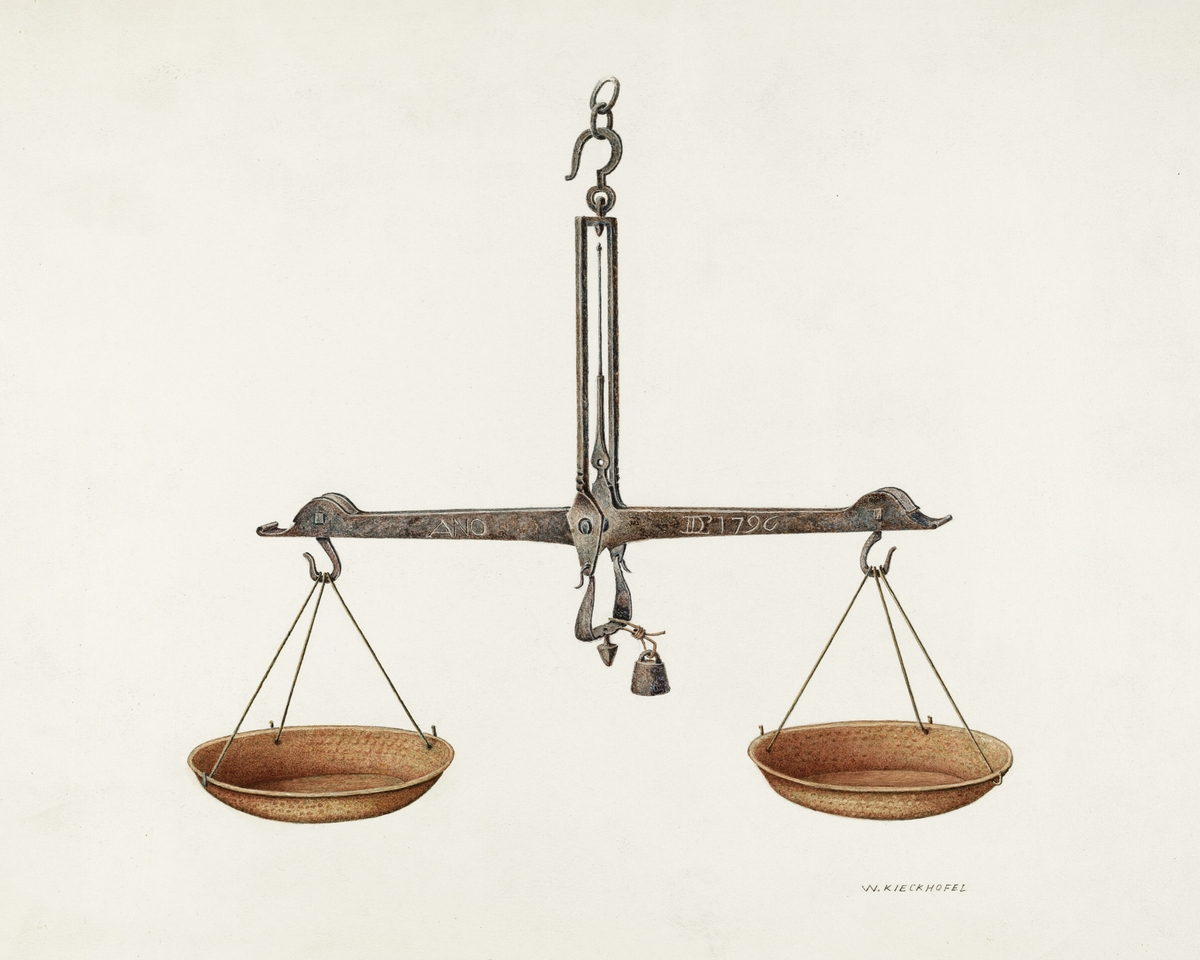
\includegraphics[width=1\linewidth]{imagenes/balanza}

\hypertarget{para-quiuxe9n-es-esto}{%
\section*{¿Para quién es esto?}\label{para-quiuxe9n-es-esto}}
\addcontentsline{toc}{section}{¿Para quién es esto?}

Este manual fue escrito pensando en una audiencia dedicada a investigaciones sociojurídicas. Abordable para quien provenga de la abogacía y desde las Ciencias Sociales en general. Aún así, y por supuesto, todas las personas y algoritmos con capacidad de procesar lenguaje son bienvenidas.

Esperamos que el tono introductorio del texto, así como el esfuerzo puesto en explicar los conceptos con la mayor simplicidad posible, resulten de interés para un público amplio.

No hace falta ningún conocimiento previo de programación; todas las herramientas necesarias serán explicadas sobre la marcha.

\hypertarget{antes-de-empezar}{%
\section*{Antes de empezar}\label{antes-de-empezar}}
\addcontentsline{toc}{section}{Antes de empezar}

Para practicar los ejemplos que se explicarán a lo largo del libro, es necesario instalar el \href{https://cloud.r-project.org/}{lenguaje de programación R}, y la interfaz gráfica \href{https://www.rstudio.com/products/rstudio/download/}{RStudio Desktop}.

\hypertarget{quuxe9-es-la-ciencia-de-datos}{%
\chapter{¿Qué es la ciencia de datos?}\label{quuxe9-es-la-ciencia-de-datos}}

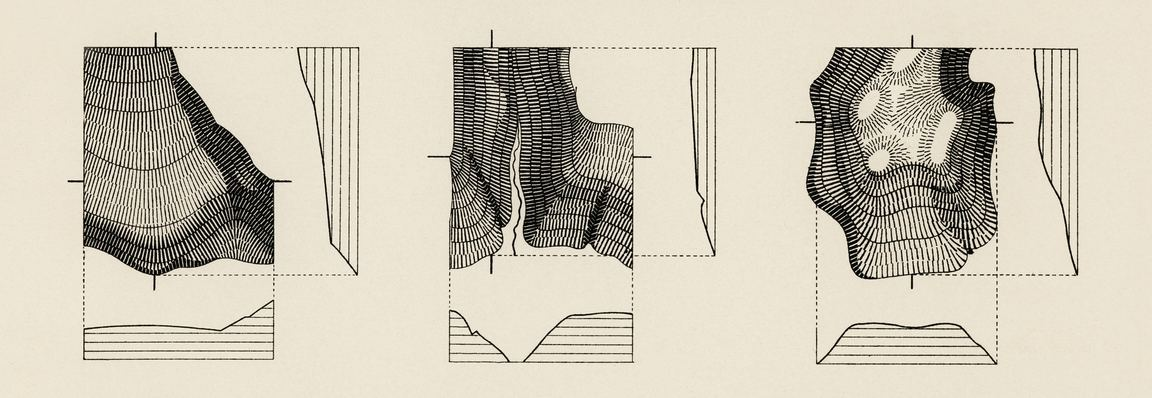
\includegraphics[width=1\linewidth]{imagenes/que_es_ciencia_de_datos}

La \emph{Big Data} ha llegado para quedarse, y asumimos que su efecto en la sociedad será permanente. Así como pasó con la escritura, los medios de comunicación o tantos otros inventos humanos de inmenso impacto cultural, el incremento en la producción y análisis computacional de grandes volúmenes de datos está transformando cada una de nuestras actividades. Algunas profesiones se ven en crisis, otras se benefician, y también se crean algunas nuevas.

Big data es un término impreciso, que se usa cuando queremos hablar de los datos que nuestra sociedad crea y procesa en forma digital, con cada vez más creciente velocidad, volumen, y variedad.

En forma acorde, \emph{data scientist} o ``científico de datos'' es también una profesión, o una actividad, que aún no está definida con toda claridad. El término, que abarca a quienes en forma cotidiana aplican técnicas de programación para analizar datos, no existía antes del 2008. Sólo cuatro años después la publicación Harvard Business Review agitó las aguas al declarar a la científicos de datos como la profesión ``más sexy del siglo XXI''\footnote{Véase ``Data Scientist: The Sexiest Job of the 21st Century'', \url{https://hbr.org/2012/10/data-scientist-the-sexiest-job-of-the-21st-century}}. Títulos exagerados aparte\footnote{Sólo un par de años después llegó la confesión: ``The Sexiest Job of the 21st Century is Tedious, and that Needs to Change'', \url{https://hbr.org/2012/10/data-scientist-the-sexiest-job-of-the-21st-century}}, lo que es seguro es que la disciplina ofrece un conjunto cada vez más maduro de saberes orientados a explotar datos para extraer conocimiento. Las técnicas y principios que la comunidad de la ciencia de datos ha desarrollado pueden ser aprovechados en muchos ámbitos. Entre ellos, el de las ciencias sociales, que también están en una etapa de transformación e incorporan la programación analítica como un recurso cada vez extendido.

Avanzar las fronteras de la ciencia de datos, crear los algoritmos y técnicas informáticas que abren nuevas posibilidades de análisis es una tarea compleja, llevada a cabo por especialistas con profundos conocimientos de matemática. Y sin embargo ``usar'' la ciencia de datos, aplicar sus principios para resolver problemas complejos, es bastante más fácil. Para empezar sólo necesitamos paciencia para aprender algunos conceptos fundamentales de programación y estadística, empleándolos para entender y comunicar con datos. De eso se trata este libro.

\hypertarget{quuxe9-significa-hacer-ciencia-de-datos}{%
\section{¿Qué significa hacer ciencia de datos?}\label{quuxe9-significa-hacer-ciencia-de-datos}}

Ya dijimos que la ciencia de datos se trata de emplear técnicas de programación para analizar datos. Pero no es sólo eso; la ciencia de datos aplicada requiere el desarrollo de habilidades en cuatro áreas:

\begin{itemize}
\item
  \textbf{Programación}. Según la definición que hemos aceptado, todo científico de datos utiliza la programación para explicar a las computadoras lo que necesita de ellas. Al hacerlo, emplea el ``pensamiento computacional'': la habilidad de reducir una tarea compleja a una serie de pasos que pueden resolverse con código interpretado por una computadora. Aclaremos por si hiciera falta que no todos los problemas son solubles por medios computacionales, pero muchos lo son, al menos en parte. El científico de datos pone en práctica algunas técnicas de programación (o muchas, según el grado de especialización) para resolver problemas que sería impráctico abordar de otro modo.
\item
  \textbf{Estadística}. ¡Inescapable! También poderosa, a veces anti-intuitiva, cuando tenemos suerte reveladora. La estadística es muchas cosas, pero -a pesar de su mala fama- aburrida jamás. Sólo es cuestión de amigarse con ella. Vamos a necesitarla para extraer conocimiento de los datos. Es sorprendente lo mucho que puede lograrse con sólo unos rudimentos (media, mediana, desvío estándar y cuartiles) y de allí en más sólo es cuestión de profundizar paso a paso.
\item
  \textbf{Comunicación}. Un científico de datos combina habilidades ``duras'' con otras que requieren empatizar con los demás: las que se relacionan con la comunicación y la colaboración interdisciplinaria. Encontrar la forma de explicar procesos complejos, de llevar las revelaciones de un modelo estadístico a términos que tengan sentido para un público amplio, crear visualizaciones que permitan a terceros ``leer'' los datos y sacar conclusiones por su cuenta. Parte de hacer ciencia de datos es saber cómo discutir los datos usados y los resultados obtenidos con un interlocutores muy diversos: audiencia general, funcionarios públicos, colegas, especialistas de otras disciplinas, etcétera.
\item
  \textbf{Conocimiento de dominio}. El conocimiento de dominio es la experiencia acumulada en un campo particular de actividad humana: agricultura, relaciones públicas, física cuántica, crianza de niños. Complementa de forma imprescindible a las habilidades analíticas. El conocimiento de dominio no sólo ayuda a discernir si las respuestas obtenidas mediante un sofisticado análisis estadístico tienen sentido. También es necesario para saber cuáles son las preguntas que deberíamos estar haciendo.
\end{itemize}

Las cuatros habilidades entran en acción en cada proyecto que involucra ciencia de datos, en mayor o menor medida de acuerdo a la etapa de análisis. Hablando de etapas, Hadley Wickham, uno de los referentes actuales en el campo, las define así:

\begin{figure}
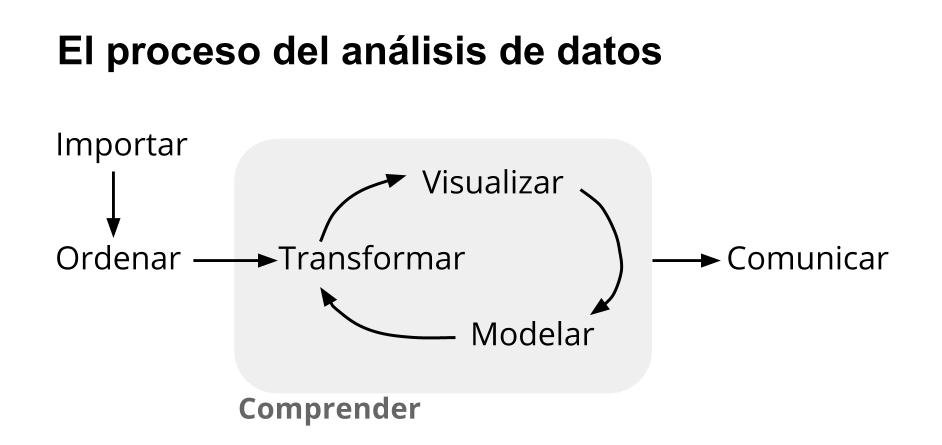
\includegraphics[width=13.08in]{imagenes/proceso_ciencia_datos} \caption{etapas en la aplicación de ciencia de datos}\label{fig:unnamed-chunk-4}
\end{figure}

Y todo ello llevado a cabo mediante la programación, por supuesto.

A lo largo de los capítulos de este libro vamos a aprender técnicas de programación que nos permitan atravesar cada uno de los pasos del proceso, y al hacerlo estaremos ejercitando las cuatro habilidades que involucra la ciencia de datos.

Allá vamos.

\hypertarget{una-presentaciuxf3n-a-toda-marcha-de-r}{%
\chapter{Una presentación a toda marcha de R}\label{una-presentaciuxf3n-a-toda-marcha-de-r}}

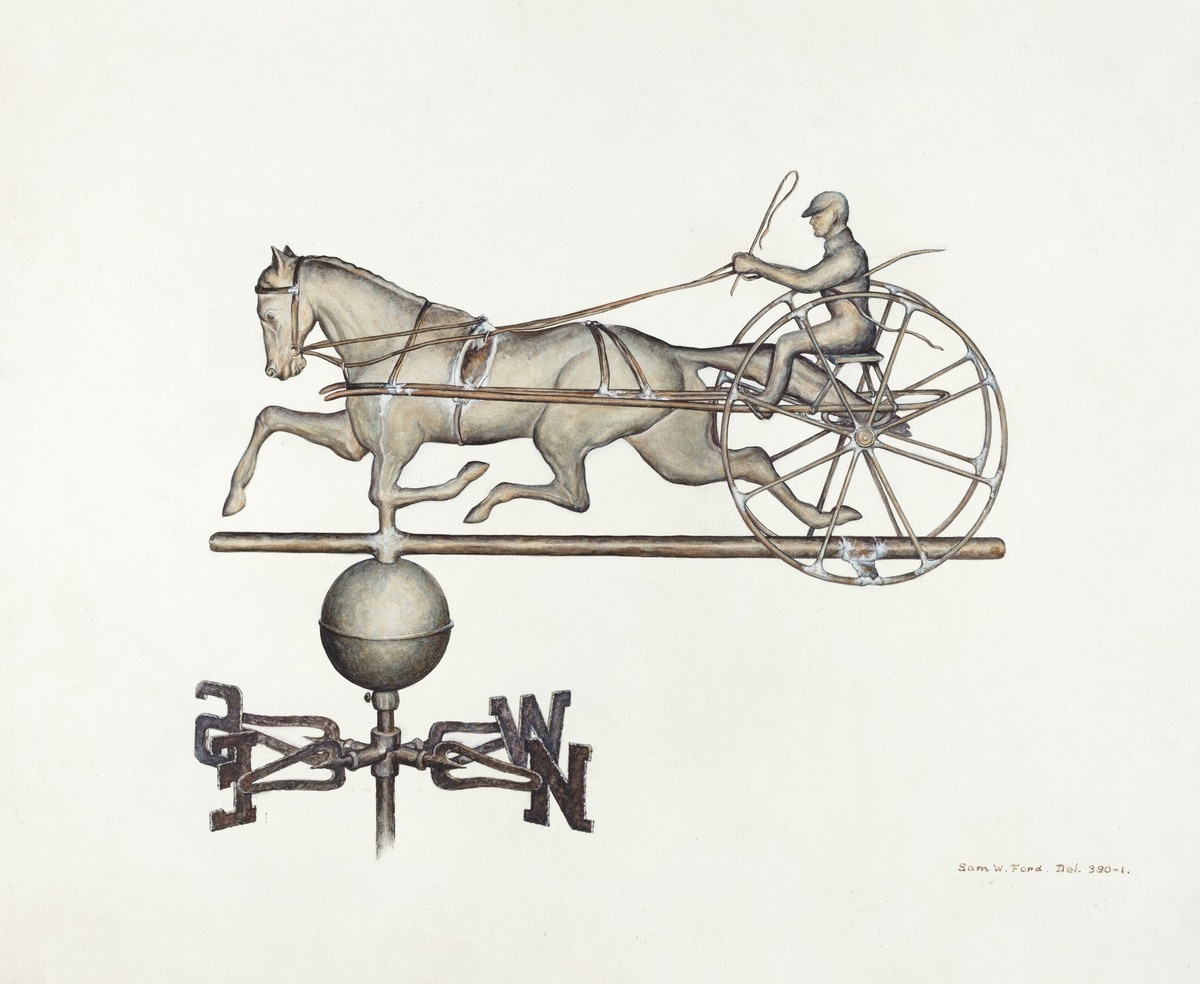
\includegraphics[width=1\linewidth]{imagenes/a_toda_marcha}

\texttt{R} es un lenguaje de programación especializado en análisis y visualización de datos. Es un producto de código abierto, lo cual significa que cualquier persona puede usarlo y modificarlo sin pagar licencias ni costos de adquisición de ningún tipo.

Expertos de todo el mundo colaboran en forma activa con el proyecto, no sólo desarrollando el lenguaje en sí (llamado ``R base''), sino también extendiéndolo con nuevas habilidades que pueden ser incorporadas por los usuarios finales en forma de ``paquetes'' instalables.

La calidad del lenguaje en sí, de los paquetes que le agregan un sinfín de funciones (desde algoritmos de inteligencia artificial hasta mapas interactivos) y de la comunidad de usuarios que comparte información en foros y blogs, ha hecho de R uno de los lenguajes de programación más populares del mundo. En el campo del análisis de datos, es la herramienta por excelencia en muchas universidades, empresas de tecnología, y redacciones de periodismo de datos.

\hypertarget{nuestro-primer-proyecto-en-r}{%
\section{Nuestro primer proyecto en R}\label{nuestro-primer-proyecto-en-r}}

A continuación reproduciremos un ejercicio paso a paso, para ilustrar la potencia de una herramienta de análisis como R. Que nadie se preocupe si algunas de las operaciones parecen no tener sentido, o resultan arbitrarias. ¡Es normal! Nadie aprende un lenguaje en 10 minutos, sea R o esperanto. La idea es tener exposición temprana a un caso de uso interesante, usando datos reales. Y que nos sirva como motivación para practicar luego ejercicios básicos que son muy necesarios pero, a veces, no tan emocionantes.

\hypertarget{a-investigar-cual-es-la-diferencia-en-mortalidad-infantil-entre-el-sur-y-el-norte-de-la-ciudad-autuxf3noma-de-buenos-aires}{%
\subsection{A investigar: ¿Cual es la diferencia en mortalidad infantil entre el sur y el norte de la Ciudad Autónoma de Buenos Aires?}\label{a-investigar-cual-es-la-diferencia-en-mortalidad-infantil-entre-el-sur-y-el-norte-de-la-ciudad-autuxf3noma-de-buenos-aires}}

Buenos Aires es una ciudad que desde hace décadas presenta una \href{https://elpais.com/internacional/2016/10/16/argentina/1476629610_416732.html}{marcada polarización} entre sus barrios del sur, relativamente menos desarrollados, y los del norte donde el nivel socioeconómico y la calidad de vida son mayores.

\begin{figure}
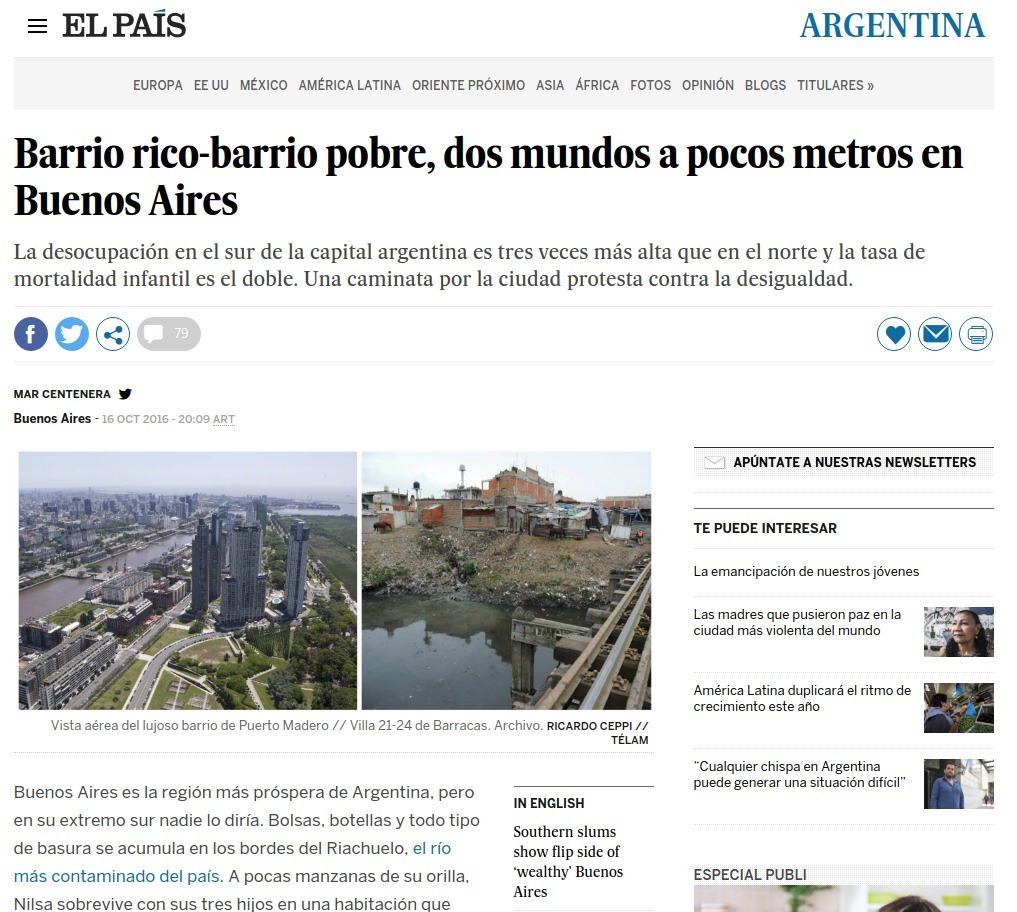
\includegraphics[width=1\linewidth]{imagenes/noticia_caba} \caption{Artículo en la edición online de El País}\label{fig:unnamed-chunk-6}
\end{figure}

Uno de los aspectos más lamentables de la disparidad norte-sur, y sin duda de los que más polémica y acusaciones cruzadas ha generado, es la diferencia en la tasa de mortalidad infantil de acuerdo a la región de la ciudad.

¿Qué tan grande es esa diferencia? ¿Cómo se distribuye geográficamente?

Vamos a utilizar R para responder esas preguntas y visualizar los resultados de nuestro análisis, utilizando como fuente cifras oficiales publicada por la ciudad.

\hypertarget{crear-un-proyecto-en-rstudio}{%
\subsection{Crear un proyecto en RStudio}\label{crear-un-proyecto-en-rstudio}}

El primer paso es ejecutar RStudio, que ya deberíamos tener disponible en nuestro sistema.

Una vez abierta la interfaz gráfica, creamos un proyecto nuevo, cliqueando en \texttt{File\ -\textgreater{}\ New\ Project...\ -\textgreater{}\ New\ Directory\ -\textgreater{}\ \ New\ Project}. En la ventana que surge, elegir un nombre para el proyecto (por ejemplo, ``Practicando R'') y finalizar la operación cliqueando en \texttt{Create\ project}.

Utilizar proyectos nos permite continuar otro día desde donde dejamos la tarea al terminar una sesión. Es sólo cuestión de recuperar el proyecto deseado la próxima vez que abrimos RStudio, cliqueando en \texttt{File\ -\textgreater{}\ Recent\ Projects\ -\textgreater{}\ "nombre\ de\ mi\ proyecto"}.

Por ahora, sigamos trabajando. Vamos a crear un ``script''. Un script, como su nombre en inglés lo indica, es un guión; una serie de pasos que escribimos para que nuestra computadora ejecute en secuencia. Cliqueamos en \texttt{File\ -\textgreater{}\ New\ File\ -\textgreater{}\ R\ Script}. De inmediato se abre una ventana con un editor de texto. ¡Ahora empieza la acción!

\hypertarget{escribiendo-un-script}{%
\subsection{Escribiendo un script}\label{escribiendo-un-script}}

Aprovechemos para dar un nombre a los áreas que vemos en RStudio:

\begin{figure}
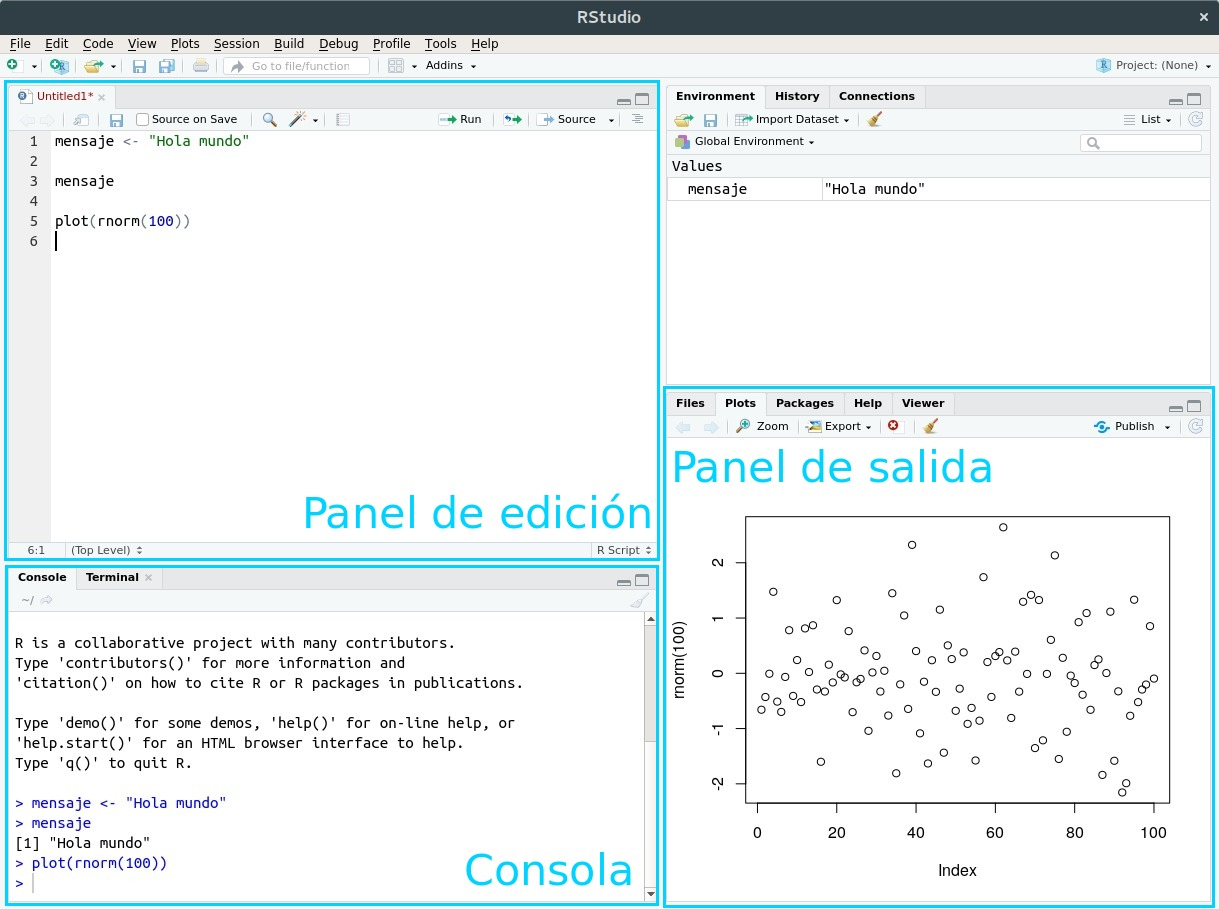
\includegraphics[width=1\linewidth]{imagenes/Interfaz_RStudio} \caption{La interfaz de RStudio}\label{fig:unnamed-chunk-7}
\end{figure}

Vamos a escribir nuestro código (las instrucciones que \texttt{R} entiende) en el panel de edición. Los resultados van a aparecer en la consola (cuando se trate de texto) o en el panel de salida (cuando produzcamos gráficos)

Por ejemplo, podemos escribir el panel de edición la instrucción para mostrar el resultado de una operación matemático:

\begin{Shaded}
\begin{Highlighting}[]
\FunctionTok{sqrt}\NormalTok{(}\DecValTok{144}\NormalTok{)}
\end{Highlighting}
\end{Shaded}

\texttt{sqrt()} es una \emph{función}. En el mundo de la programación, las funciones son secuencias de código ya listas para usar, que realizan tareas útiles. Por ejemplo, mostrar algo en pantalla. En nuestro caso, completamos la función con algo más: un \emph{parámetro}, pues así se le llama a los valores que una función espera de parte del usuario para saber que hacer. La función \texttt{sqrt()} espera que le demos un número para el cual calcular su raíz cuadrada (\emph{square root} en inglés), y eso hicimos: le pasamos cómo parámetro \texttt{144}, un número. Los parámetros siempre se escriben entre paréntesis, a continuación del nombre de la función.

Ahora vamos a aprender la combinación de teclas más importante al usar RStudio: \texttt{Ctrl} + \texttt{Enter}. Presionar \texttt{Ctrl} + \texttt{Enter} al terminar de escribir una instrucción hace que RStudio la ejecute de inmediato, y espere en la siguiente instrucción, si la hubiera.

También podemos buscar una línea que deseemos ejecutar, posicionando el cursor de texto (que luce como una barra vertical que titila, en el panel de edición) sobre ella. Si a continuación pulsamos \texttt{Ctrl} + \texttt{Enter}, la línea será ejecutada y el cursor se moverá sólo hasta la siguiente línea, listo para repetir el proceso.

La modalidad de ejecución línea por línea es muy útil para lo que se llama ``análisis interactivo''. Uno ejecuta un comando, observa el resultado, y en base a eso decide su próxima acción: cambiar parámetros e intentarlo de nuevo, dar por buenos los resultados y usarlos para una tarea subsiguiente\ldots{} etc.

Por ejemplo, si escribimos las siguientes líneas:

\begin{Shaded}
\begin{Highlighting}[]
\FunctionTok{sqrt}\NormalTok{(}\DecValTok{144}\NormalTok{)}

\NormalTok{mensaje }\OtherTok{\textless{}{-}} \StringTok{"Hola mundo"}

\NormalTok{mensaje}
\end{Highlighting}
\end{Shaded}

\ldots y posicionamos el cursor en cualquier posición de la primera línea, para luego pulsar \texttt{Ctrl} + \texttt{Enter} tres veces, veremos que las instrucciones son ejecutadas línea a línea.

\begin{Shaded}
\begin{Highlighting}[]
\FunctionTok{sqrt}\NormalTok{(}\DecValTok{144}\NormalTok{)}
\end{Highlighting}
\end{Shaded}

\begin{verbatim}
## [1] 12
\end{verbatim}

\begin{Shaded}
\begin{Highlighting}[]
\NormalTok{mensaje }\OtherTok{\textless{}{-}} \StringTok{"Hola mundo"}
\end{Highlighting}
\end{Shaded}

\begin{Shaded}
\begin{Highlighting}[]
\NormalTok{mensaje}
\end{Highlighting}
\end{Shaded}

\begin{verbatim}
## [1] "Hola mundo"
\end{verbatim}

Dos de ellas (la primera y la última) mostraron una salida en pantalla, y la del medio, no. Esto es porque algunas operaciones entregan algo como resultado -un número, un texto, un gráfico, u otros tipos de salida que ya veremos- mientras que otras hacen su tarea silenciosamente sin expresar nada. En este caso, la operación silenciosa fue la de asignación: \texttt{mensaje\ \textless{}-\ "Hola\ mundo"} es una instrucción que le pide a R que cree una variable llamada ``mensaje'' (o que la encuentre si ya existe) y que le asigne como valor el texto ``Hola mundo''. ¿Cómo sabemos que la instrucción se llevó a cabo, a pesar de no producir una salida? En general, es un tema de confianza. Si una instrucción no genera un mensaje de error, si es silenciosa, se asume que pudo cumplir su cometido. En este caso, además lo hemos verificado. La línea final, \texttt{mensaje} pide a R que busque la variable, y muestre en pantalla su contenido (esa es una característica muy práctica del lenguaje: para saber el contenido de una variable, basta con escribirla y ejecutar la línea). Y al hacerlo, comprobamos que la variable contiene precisamente lo que hemos tipeado.

De paso, hay que mencionar que la creación y manipulación de variables es un concepto clave en programación. Trabajar con variables nos permite almacenar valores para usarlos después, además de hacer nuestro código más fácil de leer y compartir con otros, en especial cuando usamos nombres de variable auto-explicativos. Como ejemplo de ésto ultimo comparemos

\begin{Shaded}
\begin{Highlighting}[]
\NormalTok{x }\OtherTok{\textless{}{-}} \DecValTok{8} \SpecialCharTok{*} \DecValTok{6}
\NormalTok{x}
\end{Highlighting}
\end{Shaded}

\begin{verbatim}
## [1] 48
\end{verbatim}

\ldots{} con

\begin{Shaded}
\begin{Highlighting}[]
\NormalTok{ancho\_habitacion\_m }\OtherTok{\textless{}{-}} \DecValTok{8}
\NormalTok{profundiad\_habitacion\_m }\OtherTok{\textless{}{-}} \DecValTok{6}
\NormalTok{superficie\_habitacion\_m2 }\OtherTok{\textless{}{-}}\NormalTok{ ancho\_habitacion\_m }\SpecialCharTok{*}\NormalTok{ profundiad\_habitacion\_m}

\NormalTok{superficie\_habitacion\_m2}
\end{Highlighting}
\end{Shaded}

\begin{verbatim}
## [1] 48
\end{verbatim}

En su resultado ambas expresiones son iguales, dado que producen lo mismo. Pero la segunda esta escrita de una forma mucho más clara para un ser humano, que hace más fácil interpretar su lógica\ldots{} ¡está calculando la superficie en metros cuadrados de una habitación!. Es muy importante escribir nuestro código de la forma más explícita posible, aunque requiera tipear un poco más. Con ello, le hacemos la vida más fácil a otras personas que interpreten nuestros programas. Y también a nosotros mismos en el futuro, cuando debamos lidiar con un programa que escribimos tiempo atrás y del que a duras penas recordamos su lógica.

A todo esto\ldots{} ¿no se suponía que íbamos a investigar la mortalidad infantil en la Ciudad de Buenos Aires?. Suficiente introducción\ldots{} ¡allá vamos!

\hypertarget{cargar-los-datos}{%
\subsection{Cargar los datos}\label{cargar-los-datos}}

Vamos a cargar datos de mortalidad infantil, por comuna de la ciudad, en el año 2020, publicados por la \href{https://www.estadisticaciudad.gob.ar/eyc/}{Dirección General de Estadística y Censos} de Buenos Aires. El formato original de los datos es ``.xls'' (planilla de hojas de cálculo). Yo lo he convertido a .csv (``comma separated values'') un formato muy popular en el mundo de la ciencia de datos, ya que es muy fácil de manipular y compartir entre sistemas\ldots{} es posible abrir un archivo .csv hasta con el \href{https://es.wikipedia.org/wiki/Bloc_de_notas}{humilde block de notas}. Al igual que los archivos .xls, los .csv se utilizan para guardar información tabular: un rectángulo con filas y columnas. R incluye una función que lee archivos .csv, que se llama \texttt{read.csv}. La usamos así:

\begin{Shaded}
\begin{Highlighting}[]
\NormalTok{mortalidad }\OtherTok{\textless{}{-}} \FunctionTok{read.csv}\NormalTok{(}\StringTok{\textquotesingle{}https://cdaj.netlify.app/data/mortalidad\_infantil\_caba\_2020.csv\textquotesingle{}}\NormalTok{)}
\end{Highlighting}
\end{Shaded}

Obsérvese que los datos están alojados en un servidor de internet (accesibles vía una dirección web). Eso no es problema para la función \texttt{read.csv()}, que con la misma soltura lee archivos guardados en nuestra PC o publicados en un sitio \emph{online}.

Una vez leído el archivo, para ver el contenido de la variable donde guardamos el resultado -que hemos llamado \texttt{mortalidad}- sólo hace falta escribir su nombre:

\begin{Shaded}
\begin{Highlighting}[]
\NormalTok{mortalidad}
\end{Highlighting}
\end{Shaded}

\begin{verbatim}
##    Comuna Tasa2020
## 1       1      5.9
## 2       2      3.6
## 3       3      3.1
## 4       4      8.7
## 5       5      6.2
## 6       6      2.8
## 7       7      6.1
## 8       8      3.7
## 9       9      7.5
## 10     10      3.1
## 11     11      2.9
## 12     12      1.1
## 13     13      3.0
## 14     14      4.0
## 15     15      2.6
\end{verbatim}

Vemos que la tabla tiene 15 filas (una por \href{https://es.wikipedia.org/wiki/Comunas_de_la_ciudad_de_Buenos_Aires}{cada comuna de la ciudad}) y 2 columnas (una que indica la comuna, y otra con el valor de mortalidad infantil para el año 2020).

Sobre \textbf{dataframes} y \textbf{datasets}: En R, las tablas son llamadas \textbf{dataframes}. El dataframe es el objeto por excelencia del análisis de datos. En concepto, es muy similar a una tabla de Excel; ambos formatos guardan información en celdas identificadas por fila y columna. El dataframe es una estructura de datos digitales en forma de tabla.

Es probable que nos crucemos con un término similar: \textbf{dataset} (o ``data set''). Este otro anglicismo se refiere a cualquier colección de datos, también típicamente en formato de tabla, que se publica o comparte. Por ejemplo si un organismo de gobierno publica sus gastos mensuales en internet, en cualquier formato fácil de descargar y abrir, decimos que ofrece ``un dataset de gastos''.

Algunas funciones útiles para explorar un dataframe son \texttt{dim()}, que nos da las dimensiones del dataframe (cantidad de filas y columnas), \texttt{names()} que nos dice como se llaman sus columnas (que en general representan variables), y \texttt{head()} que nos permite echar un vistazo rápido al contenido, mostrando sólo las seis primeras filas (ésto es útil porque con frecuencia trabajamos con dataframes que contienen miles o millones de filas, por lo que no tiene sentido tratar de volcar todas en pantalla).

\begin{Shaded}
\begin{Highlighting}[]
\FunctionTok{dim}\NormalTok{(mortalidad)}
\end{Highlighting}
\end{Shaded}

\begin{verbatim}
## [1] 15  2
\end{verbatim}

\begin{Shaded}
\begin{Highlighting}[]
\FunctionTok{names}\NormalTok{(mortalidad)}
\end{Highlighting}
\end{Shaded}

\begin{verbatim}
## [1] "Comuna"   "Tasa2020"
\end{verbatim}

\begin{Shaded}
\begin{Highlighting}[]
\FunctionTok{head}\NormalTok{(mortalidad)}
\end{Highlighting}
\end{Shaded}

\begin{verbatim}
##   Comuna Tasa2020
## 1      1      5.9
## 2      2      3.6
## 3      3      3.1
## 4      4      8.7
## 5      5      6.2
## 6      6      2.8
\end{verbatim}

\hypertarget{visualizaciuxf3n-la-exploraciuxf3n-gruxe1fica-de-la-informaciuxf3n}{%
\section{Visualización: la exploración gráfica de la información}\label{visualizaciuxf3n-la-exploraciuxf3n-gruxe1fica-de-la-informaciuxf3n}}

Ahora es vamos a pisar el acelerador. Insisto: nadie debe preocuparse si algunos conceptos parecen ser demasiado complejos. En las próximas secciones practicaremos de forma gradual las técnicas que vamos a usar ahora, y todo tendrá sentido -¡lo prometo!. Pero antes, seamos un poquito irresponsables con el poder de R y empleemos un arsenal sofisticado de herramientas para ver de que somos capaces.

En la introducción hablamos de los paquetes, conjuntos de programas que extienden la funcionalidad de R. Vamos a cargar uno de los paquetes más usados, \href{https://www.tidyverse.org/}{\texttt{tidyverse}}. Tidyverse incluye una gran cantidad de funciones diseñadas por y para practicantes de la ciencia de datos. Estas funciones comparten una filosofía y una sintaxis común, por lo que al aprender una en cierto modo aprendemos a usar todas. El valor que aportan es que, sin dudas, ayudan a realizar de manera más fácil las tareas típicas de la ciencia de datos: importar, limpiar, comprender y comunicar datos.

Si acabamos de instalar R y RStudio, el paquete aún no estará disponible en nuestro sistema. Para instalarlo, usamos la función \texttt{install.packages()} y le pasamos el nombre del paquete deseado, ``tidyverse'', entre comillas.

\begin{Shaded}
\begin{Highlighting}[]
\FunctionTok{install.packages}\NormalTok{(}\StringTok{"tidyverse"}\NormalTok{)}
\end{Highlighting}
\end{Shaded}

De aquí en más, podremos activar el conjunto de funciones que provee \texttt{tidyverse} cada vez que queramos. Para eso, lo invocamos con la función \texttt{library()}:

\begin{Shaded}
\begin{Highlighting}[]
\FunctionTok{library}\NormalTok{(tidyverse)}
\end{Highlighting}
\end{Shaded}

\ldots{} y listo para usar. La razón por la cual activamos tidyverse es que en este momento nos vienen bien dos de sus funciones: \texttt{mutate()} para modificar valores, y \texttt{ggplot()} para hacer gráficos.

Bien, llega la hora de los gráficos. Vamos a llamar a la función \texttt{ggplot()}, una auténtica navaja suiza para la visualización.

Por ejemplo, veamos a cuanto asciende la tasa de mortalidad infantil en cada comuna durante 2020:

\begin{Shaded}
\begin{Highlighting}[]
\FunctionTok{ggplot}\NormalTok{(mortalidad) }\SpecialCharTok{+}
    \FunctionTok{geom\_col}\NormalTok{(}\FunctionTok{aes}\NormalTok{(}\AttributeTok{x =} \FunctionTok{factor}\NormalTok{(Comuna), }\AttributeTok{y =}\NormalTok{ Tasa2020))}
\end{Highlighting}
\end{Shaded}

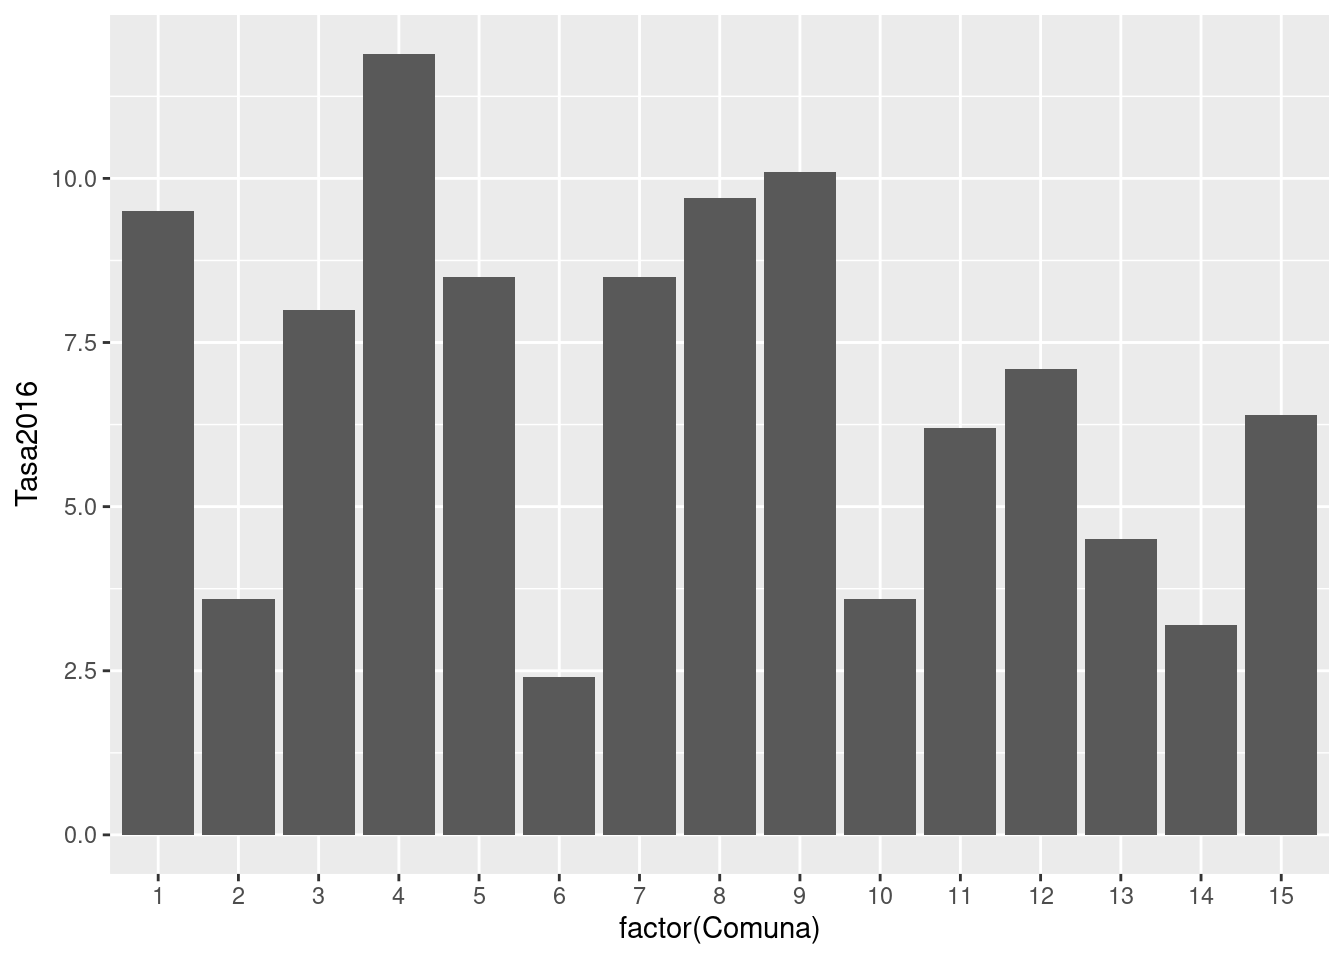
\includegraphics{CD_AJ_files/figure-latex/unnamed-chunk-20-1.pdf}

Para realizar una visualización con ésta herramienta, siempre se comienza con la función \texttt{ggplot()}, que crea un eje de coordenadas sobre el cual se pueden agregar capas. El primer parámetro que recibe \texttt{ggplot()} es el dataframe que queremos usar para el gráfico; en nuestro caso, \texttt{ggplot(mortalidad)}. Ejecutar sólo \texttt{ggplot(mortalidad)} nos devuelve un gráfico vacío; la gracia está en agregar una o más capas especificando cómo queremos mostrar los datos. Estas capas se agregan con un signo \texttt{+}.

En nuestro ejemplo, \texttt{geom\_col()} crea columnas cuya posición en el eje de las x depende de la variable ``Comuna'', mientas que la altura (posición en el eje de las y) depende del valor de la variable ``Tasa2020''. Existen muchas funciones de tipo ``\emph{geom\_XXX}'', que agregan distintas clases de capas al gráfico: \texttt{geom\_point}, \texttt{geom\_polygon}, \texttt{geom\_text} y muchos, muchos más que iremos viendo más adelante.

Cada función ``\emph{geom\_}'' toma como parámetro un conjunto de definiciones ``estéticas'' que le indican una variable a graficar (``mortalidad'' en nuestro caso), cómo (color, tamaño, etc) y dónde (posición x, posición y del eje). Estos parámetros van siempre dentro de una función auxiliar, \texttt{aes()}. En nuestro ejemplo, \texttt{geom\_col(aes(x\ =\ factor(Comuna),\ y\ =\ Tasa2020))}.

No se preocupen que iremos practicando el uso de ggplot, y su uso se volverá familiar.

En cuanto al gráfico que hemos creado, podemos observar que entre las 15 comunas en la ciudad, la tasa de mortalidad tiene un rango que va de un poco menos de 1,1 a un poco más de 8,7 (esto es, muertes antes del año de vida por cada 10.000 nacimientos).

Pero no se distingue aquello que queríamos comprender: la diferencia entre el norte y el sur de la ciudad. Necesitamos contexto geográfico.

\hypertarget{haciendo-mapas}{%
\subsection{Haciendo mapas}\label{haciendo-mapas}}

Vamos a presentar un paquete más, el último para éste capítulo: \href{https://r-spatial.github.io/sf/}{\texttt{sf}}. Quizás algunos tengan experiencia con sistemas de información geográfica (GIS por sus siglas en inglés), al estilo de \href{https://qgis.org/en/site/}{QGIS} o \href{https://www.arcgis.com/features/index.html}{ArcGIS}, que permiten crear, manipular y combinar archivos con datos espaciales para producir mapas que pueden ser simples o en extremo sofisticados. En R, el paquete \texttt{sf} brinda herramientas que permiten realizar tares similares.

Nuestro objetivo es obtener un mapa de la ciudad de Buenos Aires con sus comunas.

Primero, instalamos \texttt{sf} en caso de que aún no lo hayamos hecho.

\begin{Shaded}
\begin{Highlighting}[]
\FunctionTok{install.packages}\NormalTok{(}\StringTok{"sf"}\NormalTok{)}
\end{Highlighting}
\end{Shaded}

Vale la pena insistir: Sólo es necesario instalar los paquetes una vez. De aquí en más, cada vez que queramos echar mano a las funciones incluidas en \texttt{sf}, sólo necesitamos activarlo pues ya estará listo en nuestro sistema. Pedimos a R que active el paquete así:

\begin{Shaded}
\begin{Highlighting}[]
\FunctionTok{library}\NormalTok{(sf)}
\end{Highlighting}
\end{Shaded}

Luego, cargamos un archivo georeferenciado con las comunas de la Ciudad Autónoma de Buenos Aires, disponible online en formato \href{https://es.wikipedia.org/wiki/GeoJSON}{\emph{geojson}}, un estándar de representación de datos geográficos que es fácil de usar:

\begin{Shaded}
\begin{Highlighting}[]
\NormalTok{comunas }\OtherTok{\textless{}{-}} \FunctionTok{st\_read}\NormalTok{(}\StringTok{\textquotesingle{}https://bitsandbricks.github.io/data/CABA\_comunas.geojson\textquotesingle{}}\NormalTok{)}
\end{Highlighting}
\end{Shaded}

\begin{verbatim}
## Reading layer `CABA_comunas' from data source 
##   `https://bitsandbricks.github.io/data/CABA_comunas.geojson' 
##   using driver `GeoJSON'
## Simple feature collection with 15 features and 4 fields
## Geometry type: MULTIPOLYGON
## Dimension:     XY
## Bounding box:  xmin: -58.53152 ymin: -34.70529 xmax: -58.33514 ymax: -34.52754
## Geodetic CRS:  WGS 84
\end{verbatim}

Al igual que cuando usamos \texttt{read.csv()} para leer un archivo .csv y cargarlo como un dataframe, el comando \texttt{st\_read()} hace lo propio con archivos de información geográfica, conocidos en la jerga como ``shapefiles''. El resultado también es un dataframe, por lo cual podemos practicar el uso de las funciones que ya aprendimos, como dim(), names() y head().

\begin{Shaded}
\begin{Highlighting}[]
\FunctionTok{dim}\NormalTok{(comunas)}
\end{Highlighting}
\end{Shaded}

\begin{verbatim}
## [1] 15  5
\end{verbatim}

\begin{Shaded}
\begin{Highlighting}[]
\FunctionTok{names}\NormalTok{(comunas)}
\end{Highlighting}
\end{Shaded}

\begin{verbatim}
## [1] "barrios"   "perimetro" "area"      "comunas"   "geometry"
\end{verbatim}

\begin{Shaded}
\begin{Highlighting}[]
\FunctionTok{head}\NormalTok{(comunas)}
\end{Highlighting}
\end{Shaded}

\begin{verbatim}
## Simple feature collection with 6 features and 4 fields
## Geometry type: MULTIPOLYGON
## Dimension:     XY
## Bounding box:  xmin: -58.4627 ymin: -34.6625 xmax: -58.33514 ymax: -34.56935
## Geodetic CRS:  WGS 84
##                                                                        barrios
## 1 CONSTITUCION - MONSERRAT - PUERTO MADERO -  RETIRO - SAN NICOLAS - SAN TELMO
## 2                                                                     RECOLETA
## 3                                                    BALVANERA - SAN CRISTOBAL
## 4                           BARRACAS - BOCA - NUEVA POMPEYA - PARQUE PATRICIOS
## 5                                                              ALMAGRO - BOEDO
## 6                                                                    CABALLITO
##   perimetro     area comunas                       geometry
## 1  35572.65 17802807       1 MULTIPOLYGON (((-58.36854 -...
## 2  21246.61  6140873       2 MULTIPOLYGON (((-58.39521 -...
## 3  10486.26  6385991       3 MULTIPOLYGON (((-58.41192 -...
## 4  36277.44 21701236       4 MULTIPOLYGON (((-58.3552 -3...
## 5  12323.47  6660526       5 MULTIPOLYGON (((-58.41287 -...
## 6  10990.96  6851029       6 MULTIPOLYGON (((-58.43061 -...
\end{verbatim}

Podemos ver que el dataframe contiene 15 filas y 5 columnas. Una fila por comuna (es razonable!) y 5 columnas: ``barrios'', ``perímetro'', ``area'', ``comunas'' y ``geometry''. Nuestro vistazo mediante head() permite asumir que ``barrios'' informa los barrios que componen cada comuna, mientras que perímetro y área informan sobre las dimensiones del polígono cubierto por cada comuna. La columna ``geometry'' aparece en todos los dataframes de tipo espacial, y es la que contiene los datos con sus coordenadas geográficas.

Y hablando de coordenadas, generar un mapa a partir de un dataframe espacial creado por sf es muy fácil con la ayuda de ggplot

\begin{Shaded}
\begin{Highlighting}[]
\FunctionTok{ggplot}\NormalTok{(comunas) }\SpecialCharTok{+}
    \FunctionTok{geom\_sf}\NormalTok{()}
\end{Highlighting}
\end{Shaded}

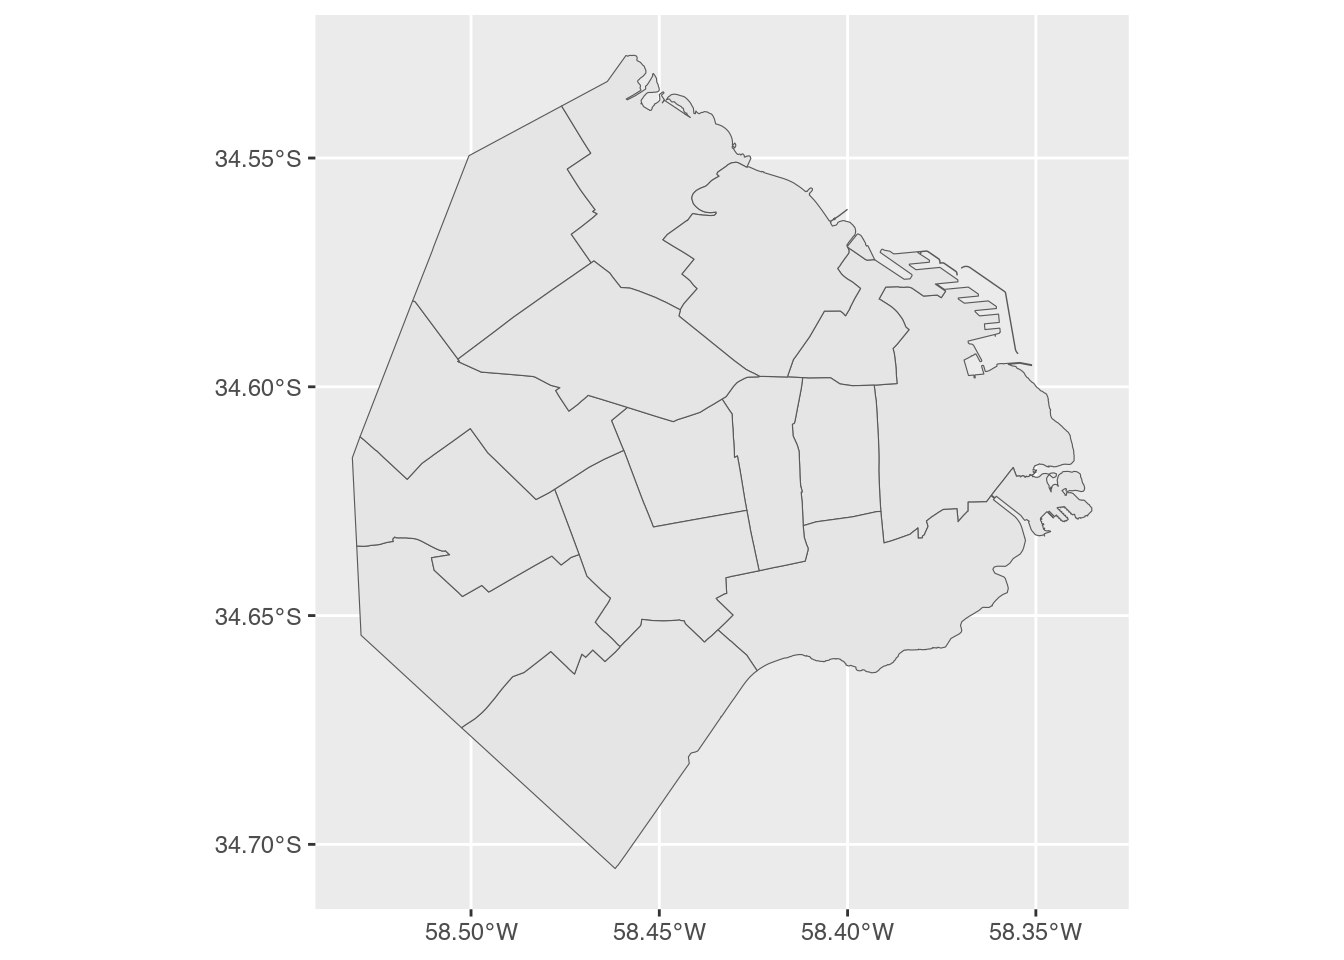
\includegraphics{CD_AJ_files/figure-latex/unnamed-chunk-25-1.pdf}

Si queremos agregar una leyenda al mapa que identifique cada comuna con su número, usamos:

\begin{Shaded}
\begin{Highlighting}[]
\FunctionTok{ggplot}\NormalTok{(comunas) }\SpecialCharTok{+}
    \FunctionTok{geom\_sf}\NormalTok{(}\FunctionTok{aes}\NormalTok{(}\AttributeTok{fill =}\NormalTok{ comunas))}
\end{Highlighting}
\end{Shaded}

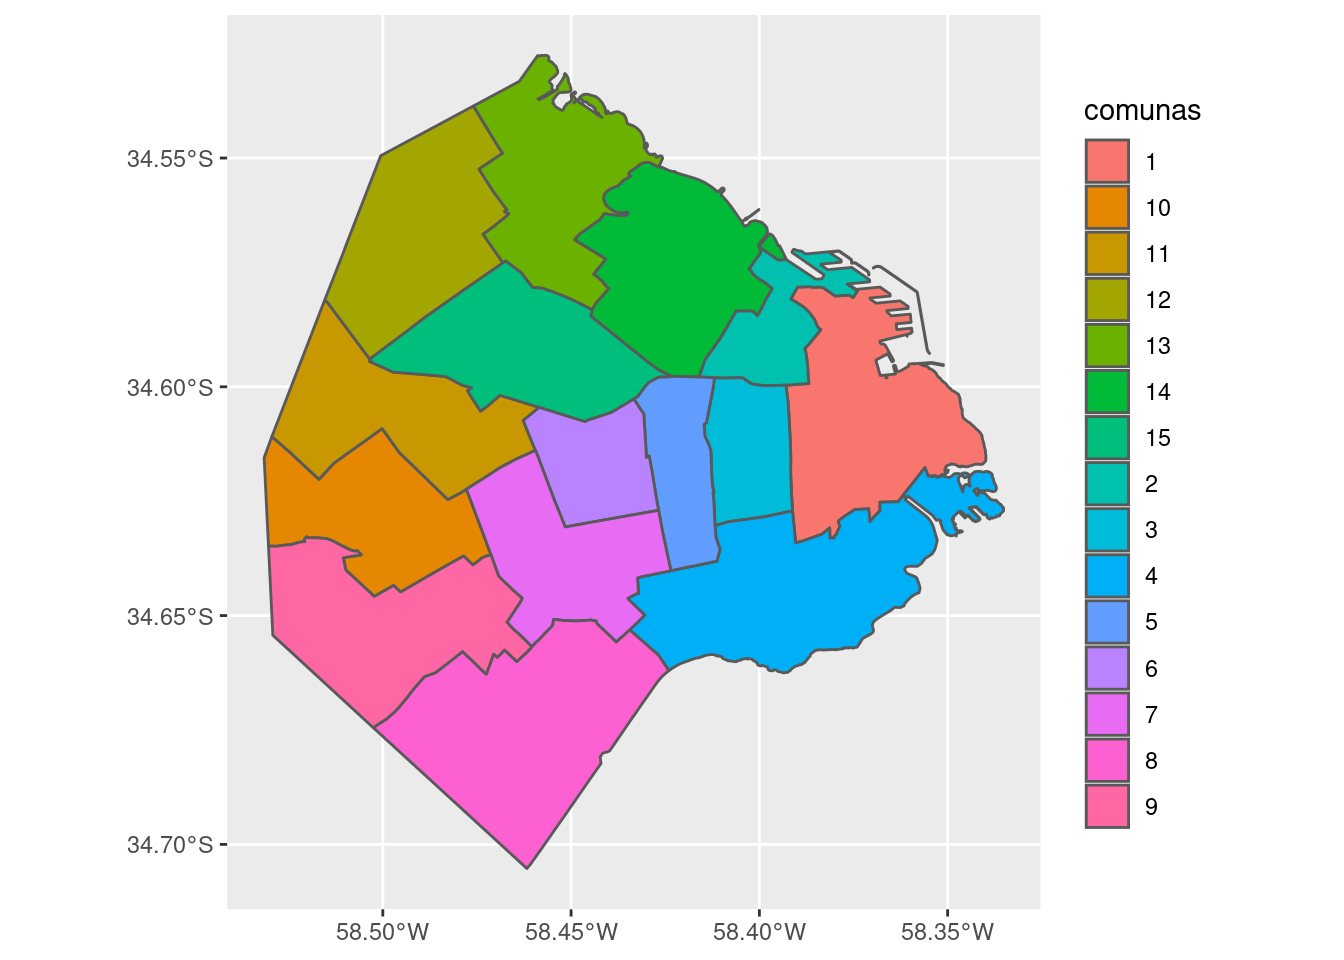
\includegraphics{CD_AJ_files/figure-latex/unnamed-chunk-26-1.pdf}

Dentro de ``aes()'' usé el parámetro ``fill'' (relleno en inglés) para pedirle a ggplot que llene cada polígono con un color distinto de acuerdo al campo ``comunas''.

Aprovechando que tenemos un mapa, deberíamos clasificar las comunas entre las que pertenecen al norte y las que pertenecen al sur de la ciudad. No hay una línea divisoria oficial, pero la traza de la Avenida Rivadavia suele ser tomada como frontera: Rivadavia es la \href{https://www.clarin.com/ediciones-anteriores/avenida-rivadaviaun-largo-recorrido-contrastes_0_B1reo181CYe.html}{``divisoria simbólica del Norte y el Sur de la Ciudad, con sus diferencias de desarrollo''}

Por esas casualidades de la vida, tengo un archivo geográfico que contiene la línea que dibuja a avenida Rivadavia al atravesar la ciudad. Lo bajamos:

\begin{Shaded}
\begin{Highlighting}[]
\NormalTok{rivadavia }\OtherTok{\textless{}{-}} \FunctionTok{st\_read}\NormalTok{(}\StringTok{\textquotesingle{}https://bitsandbricks.github.io/data/avenida\_rivadavia.geojson\textquotesingle{}}\NormalTok{)}
\end{Highlighting}
\end{Shaded}

\begin{verbatim}
## Reading layer `avenida_rivadavia' from data source 
##   `https://bitsandbricks.github.io/data/avenida_rivadavia.geojson' 
##   using driver `GeoJSON'
## Simple feature collection with 1 feature and 1 field
## Geometry type: LINESTRING
## Dimension:     XY
## Bounding box:  xmin: -58.53014 ymin: -34.63946 xmax: -58.37017 ymax: -34.60711
## Geodetic CRS:  WGS 84
\end{verbatim}

Y lo proyectamos sobre el mapa, como una capa adicional del gráfico de ggplot que definimos antes:

\begin{Shaded}
\begin{Highlighting}[]
\FunctionTok{ggplot}\NormalTok{(comunas) }\SpecialCharTok{+}
    \FunctionTok{geom\_sf}\NormalTok{(}\FunctionTok{aes}\NormalTok{(}\AttributeTok{fill =}\NormalTok{ comunas)) }\SpecialCharTok{+}
    \FunctionTok{geom\_sf}\NormalTok{(}\AttributeTok{data =}\NormalTok{ rivadavia, }\AttributeTok{color =} \StringTok{"red"}\NormalTok{)}
\end{Highlighting}
\end{Shaded}

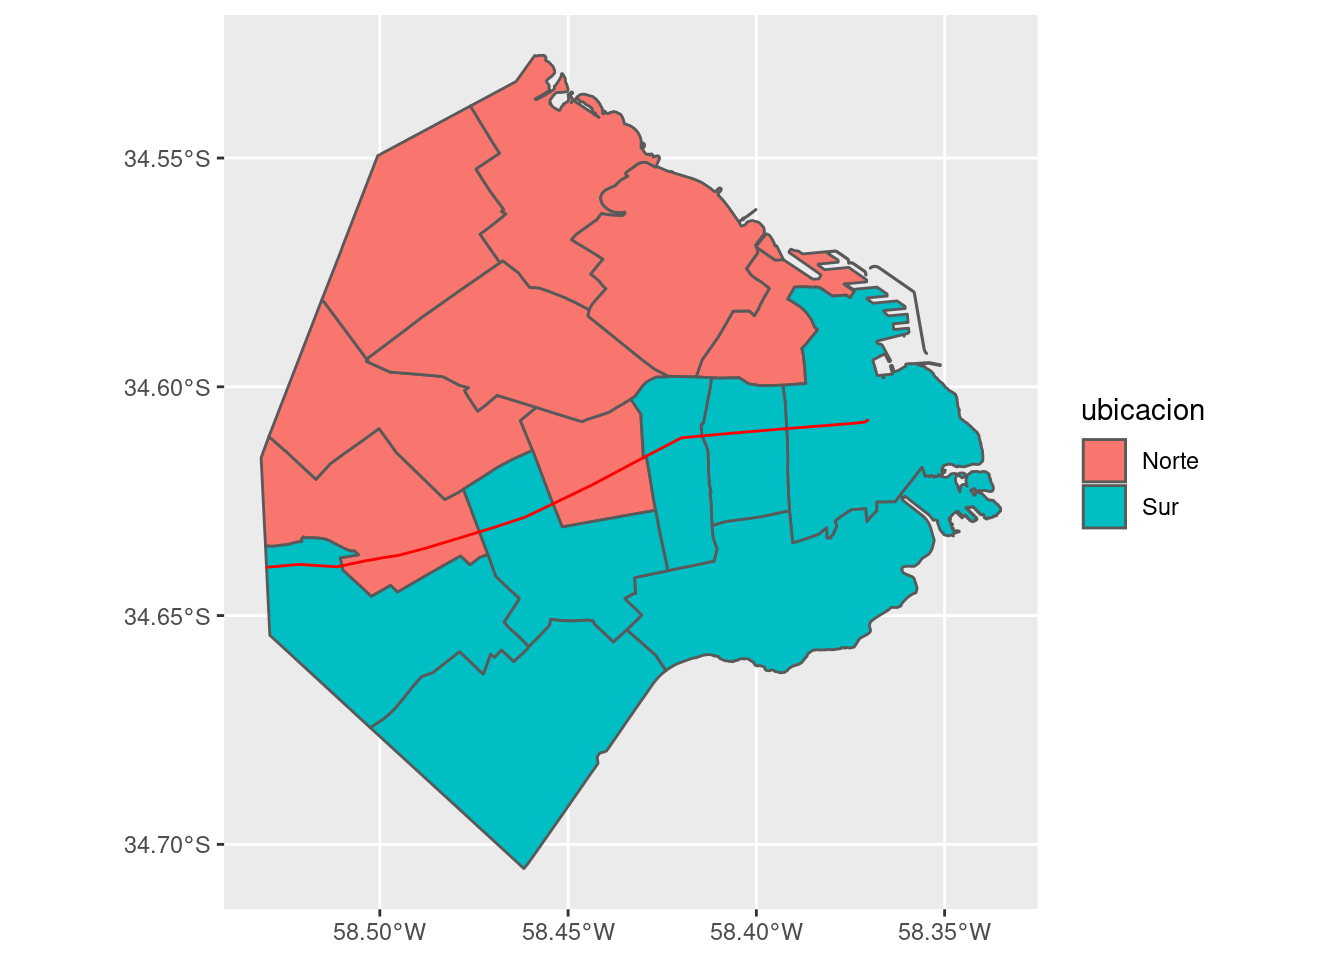
\includegraphics{CD_AJ_files/figure-latex/unnamed-chunk-28-1.pdf}

La identificación por colores no hace fácil reconocer con rapidez que número corresponde a cada comuna; es un recurso que funciona mejor con menos categorías que nuestras 15. Podríamos arreglarlo, por ejemplo evitando la codificación por color, y dibujando una etiqueta con número dibujada sobre cada comuna. ¡Pero no en este momento! En aras de la sencillez, vamos a aguzar la vista y tomar nota de cuales comunas tienen gran parte de su territorio al sur de la Avenida Rivadavia. Según mi interpretación, son las comunas 1, 3, 4, 5, 7, 8 y 9. (Hay que admitir que la comuna 1 parece estar repartida en partes más o menos iguales, pero vamos a dejársela al sur en forma arbitraria para no complicar el ejercicio).

\hypertarget{agregando-datos}{%
\subsection{Agregando datos}\label{agregando-datos}}

En este punto necesitamos una manera de ``etiquetar'' cada comuna con el punto cardinal que le toca ``Norte'' o ``Sur''. La forma más rápida es crear una lista con los atributos, y agregarla a nuestro dataframe como una nueva columna.

Podemos armar una sucesión de 15 ``etiquetas'' según el punto cardinal que le toca a cada comuna. El comando en R que ``une'' valores en conjunto se llama \texttt{c()} (viene de ``combine'', ``combinar''), y permite definir una lista de valores. Mejor dicho, un ``vector'' de valores; en el mundo de la programación, se usa la palabra vector cuando se combinan elementos del mismo tipo, y ``lista'' cuando se combina una variedad de clases: en el mismo conjunto números, textos, y otros tipos de objeto más complejos. Por ahora, no nos preocupemos por eso.

\begin{Shaded}
\begin{Highlighting}[]
\NormalTok{nueva\_columna }\OtherTok{\textless{}{-}} \FunctionTok{c}\NormalTok{(}\StringTok{"Sur"}\NormalTok{, }\StringTok{"Norte"}\NormalTok{, }\StringTok{"Sur"}\NormalTok{, }\StringTok{"Sur"}\NormalTok{, }\StringTok{"Sur"}\NormalTok{, }\StringTok{"Norte"}\NormalTok{, }\StringTok{"Sur"}\NormalTok{, }\StringTok{"Sur"}\NormalTok{, }
                   \StringTok{"Sur"}\NormalTok{, }\StringTok{"Norte"}\NormalTok{, }\StringTok{"Norte"}\NormalTok{, }\StringTok{"Norte"}\NormalTok{, }\StringTok{"Norte"}\NormalTok{, }\StringTok{"Norte"}\NormalTok{, }\StringTok{"Norte"}\NormalTok{)}

\NormalTok{nueva\_columna}
\end{Highlighting}
\end{Shaded}

\begin{verbatim}
##  [1] "Sur"   "Norte" "Sur"   "Sur"   "Sur"   "Norte" "Sur"   "Sur"   "Sur"  
## [10] "Norte" "Norte" "Norte" "Norte" "Norte" "Norte"
\end{verbatim}

Ya podemos agregar nuestra nueva columna usando una función que ya vimos, mutate(). En el dataframe, vamos a ponerle a nuestra nueva columna un nombre descriptivo, ``ubicación'' :

\begin{Shaded}
\begin{Highlighting}[]
\NormalTok{comunas }\OtherTok{\textless{}{-}} \FunctionTok{mutate}\NormalTok{(comunas, }\AttributeTok{ubicacion =}\NormalTok{ nueva\_columna)}
\end{Highlighting}
\end{Shaded}

Verifiquemos el resultado:

\begin{Shaded}
\begin{Highlighting}[]
\FunctionTok{head}\NormalTok{(comunas)}
\end{Highlighting}
\end{Shaded}

\begin{verbatim}
## Simple feature collection with 6 features and 5 fields
## Geometry type: MULTIPOLYGON
## Dimension:     XY
## Bounding box:  xmin: -58.4627 ymin: -34.6625 xmax: -58.33514 ymax: -34.56935
## Geodetic CRS:  WGS 84
##                                                                        barrios
## 1 CONSTITUCION - MONSERRAT - PUERTO MADERO -  RETIRO - SAN NICOLAS - SAN TELMO
## 2                                                                     RECOLETA
## 3                                                    BALVANERA - SAN CRISTOBAL
## 4                           BARRACAS - BOCA - NUEVA POMPEYA - PARQUE PATRICIOS
## 5                                                              ALMAGRO - BOEDO
## 6                                                                    CABALLITO
##   perimetro     area comunas                       geometry ubicacion
## 1  35572.65 17802807       1 MULTIPOLYGON (((-58.36854 -...       Sur
## 2  21246.61  6140873       2 MULTIPOLYGON (((-58.39521 -...     Norte
## 3  10486.26  6385991       3 MULTIPOLYGON (((-58.41192 -...       Sur
## 4  36277.44 21701236       4 MULTIPOLYGON (((-58.3552 -3...       Sur
## 5  12323.47  6660526       5 MULTIPOLYGON (((-58.41287 -...       Sur
## 6  10990.96  6851029       6 MULTIPOLYGON (((-58.43061 -...     Norte
\end{verbatim}

Y en el mapa:

\begin{Shaded}
\begin{Highlighting}[]
\FunctionTok{ggplot}\NormalTok{(comunas) }\SpecialCharTok{+}
    \FunctionTok{geom\_sf}\NormalTok{(}\FunctionTok{aes}\NormalTok{(}\AttributeTok{fill =}\NormalTok{ ubicacion)) }\SpecialCharTok{+}
    \FunctionTok{geom\_sf}\NormalTok{(}\AttributeTok{data =}\NormalTok{ rivadavia, }\AttributeTok{color =} \StringTok{"red"}\NormalTok{)}
\end{Highlighting}
\end{Shaded}

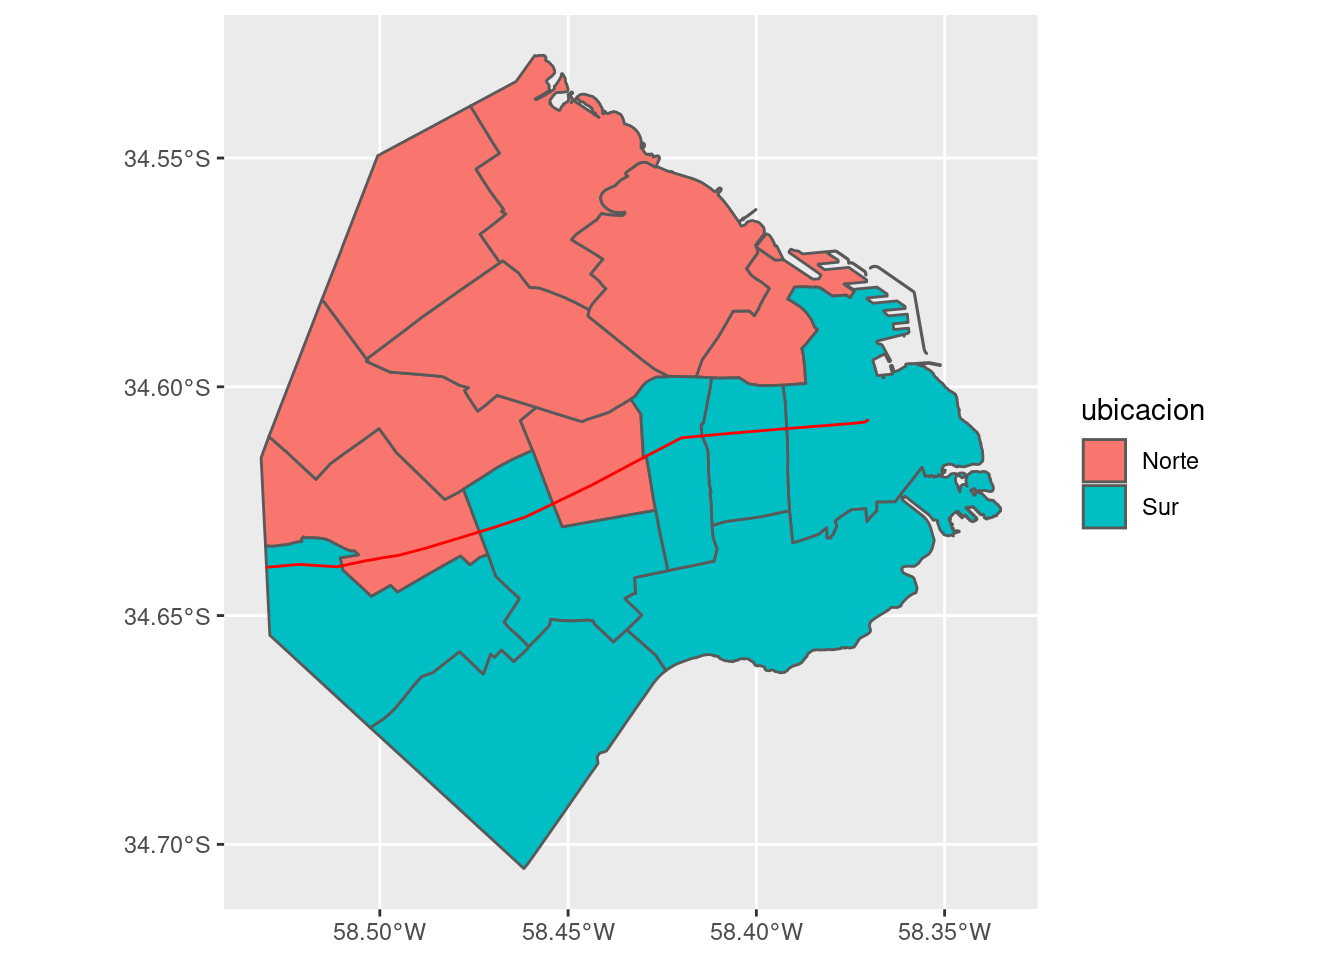
\includegraphics{CD_AJ_files/figure-latex/unnamed-chunk-32-1.pdf}

Todo en orden. Ahora hagamos lo mismo con el dataframe de mortalidad, aprovechando que lista las comunas en el mismo orden (del 1 al 15) y por lo tanto podemos ``pegarle'' el mismo vector de etiquetas con ubicación que ya preparamos.

\begin{Shaded}
\begin{Highlighting}[]
\NormalTok{mortalidad }\OtherTok{\textless{}{-}} \FunctionTok{mutate}\NormalTok{(mortalidad, ubicación }\OtherTok{=}\NormalTok{ nueva\_columna)}
                         
\FunctionTok{head}\NormalTok{(mortalidad)}
\end{Highlighting}
\end{Shaded}

\begin{verbatim}
##   Comuna Tasa2020 ubicación
## 1      1      5.9       Sur
## 2      2      3.6     Norte
## 3      3      3.1       Sur
## 4      4      8.7       Sur
## 5      5      6.2       Sur
## 6      6      2.8     Norte
\end{verbatim}

\hypertarget{el-veredicto-final}{%
\section{El veredicto final}\label{el-veredicto-final}}

Habrán notado que llegar hasta aquí tomó una buena cantidad de operaciones. En contraste, lo que estamos a punto de hacer -responder la pregunta inicial- va a ser mucho más breve. Esa vendría a ser la lección central de éste capítulo: la mayor parte del tiempo empleado en la labor de la ciencia de datos se insume en la poco glamorosa tarea de recopilar, limpiar y combinar los registros necesarios para el análisis. Como consuelo, podemos pensar en que el esfuerzo necesario para llegar a este punto nos ha dado un conocimiento de los datos (su estructura, sus limitaciones, su potencial) que no teníamos antes.

Aprovechemos entonces nuestra data limpia y ordenada, para producir un mapa que señale con color el nivel de mortalidad. Armamos un ggplot con una capa que muestra las comunas, cuyo color interior (``fill'') depende del valor de la mortalidad. Le sumamos una capa con la traza de la Avenida Rivadavia, nuestra referencia de posición, y por último definimos la paleta de colores a usar en el \emph{fill}, eligiendo una llamada ``Spectral'', que va del azul al rojo y es muy usada cuando se quiere resaltar la divergencia de una variable.

\begin{Shaded}
\begin{Highlighting}[]
\FunctionTok{ggplot}\NormalTok{(comunas) }\SpecialCharTok{+}
    \FunctionTok{geom\_sf}\NormalTok{(}\FunctionTok{aes}\NormalTok{(}\AttributeTok{fill =}\NormalTok{ mortalidad}\SpecialCharTok{$}\NormalTok{Tasa2020)) }\SpecialCharTok{+}
    \FunctionTok{geom\_sf}\NormalTok{(}\AttributeTok{data =}\NormalTok{ rivadavia, }\AttributeTok{color =} \StringTok{"red"}\NormalTok{) }\SpecialCharTok{+}
    \FunctionTok{scale\_fill\_distiller}\NormalTok{(}\AttributeTok{palette =} \StringTok{"Spectral"}\NormalTok{)}
\end{Highlighting}
\end{Shaded}

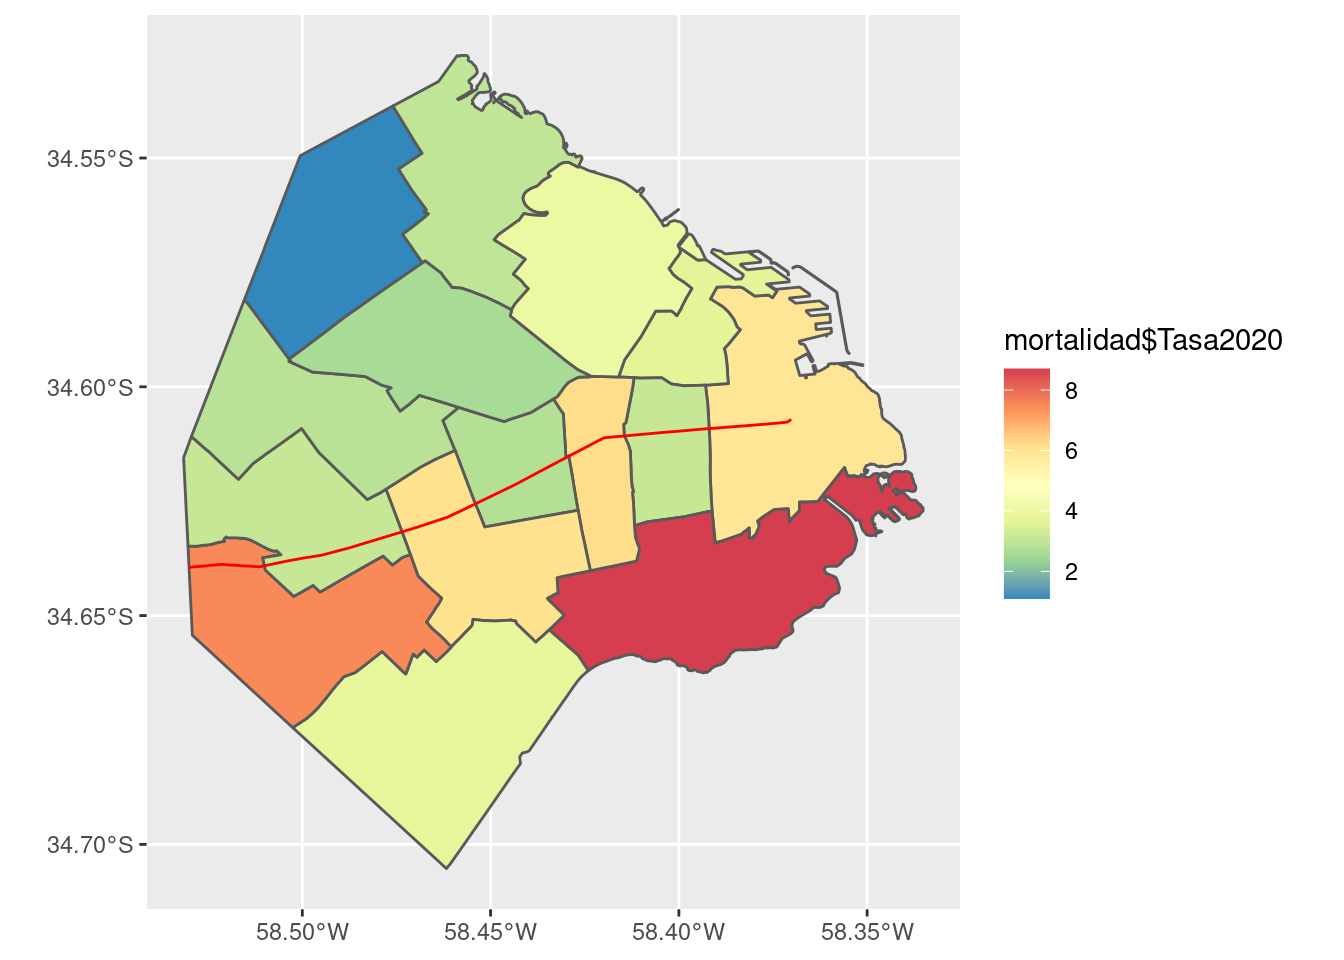
\includegraphics{CD_AJ_files/figure-latex/unnamed-chunk-34-1.pdf}

Para una comparación visual más precisa entre los valores de cada comuna, le pedimos a ggplot un gráfico de barras, con la capa \texttt{geom\_col()}. En las variables estéticas, definimos que la posición de las barras en el eje de las x estará dada por el número de cada comuna, la altura de las barras (eje y) será dada por su tasa de mortalidad, y su color de relleno (fill) dependerá de su ubicación geográfica.

\begin{Shaded}
\begin{Highlighting}[]
\FunctionTok{ggplot}\NormalTok{(mortalidad) }\SpecialCharTok{+}
    \FunctionTok{geom\_col}\NormalTok{(}\FunctionTok{aes}\NormalTok{(}\AttributeTok{x =}\NormalTok{ Comuna, }\AttributeTok{y =}\NormalTok{ Tasa2020, }\AttributeTok{fill =}\NormalTok{ ubicación)) }\SpecialCharTok{+}
    \FunctionTok{labs}\NormalTok{(}\AttributeTok{title =} \StringTok{"Mortalidad infantil en la Ciudad Autónoma de Buenos Aires"}\NormalTok{,}
         \AttributeTok{subtitle =} \StringTok{"Año 2020"}\NormalTok{,}
         \AttributeTok{y =} \StringTok{"tasa"}\NormalTok{) }
\end{Highlighting}
\end{Shaded}

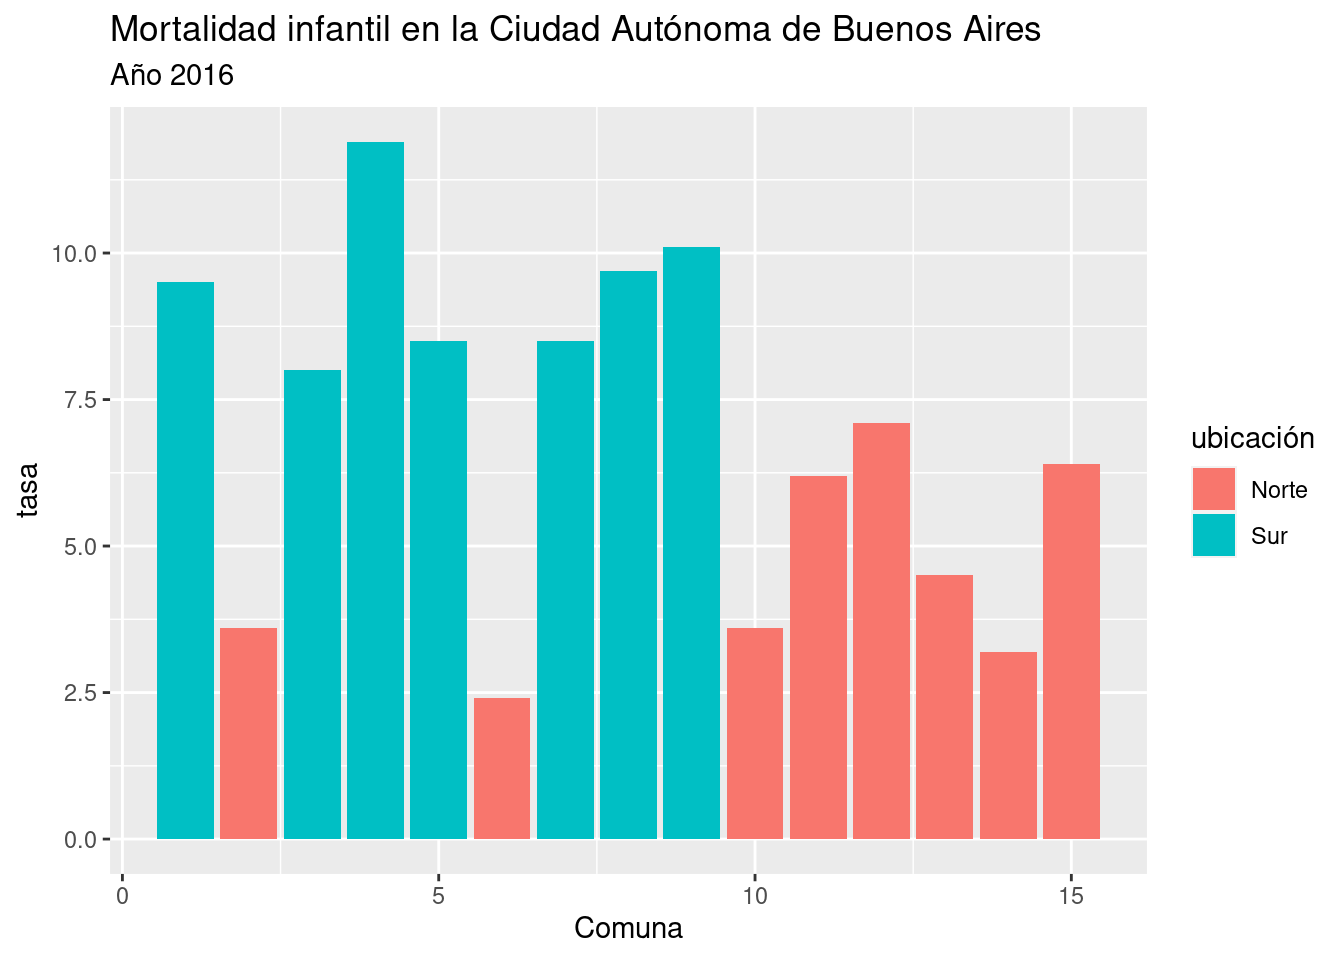
\includegraphics{CD_AJ_files/figure-latex/unnamed-chunk-35-1.pdf}

\hypertarget{cuuxe1l-es-la-diferencia-en-mortalidad-infantil-entre-el-sur-y-el-norte-de-la-ciudad-autuxf3noma-de-buenos-aires}{%
\subsection{¿Cuál es la diferencia en mortalidad infantil entre el sur y el norte de la Ciudad Autónoma de Buenos Aires?}\label{cuuxe1l-es-la-diferencia-en-mortalidad-infantil-entre-el-sur-y-el-norte-de-la-ciudad-autuxf3noma-de-buenos-aires}}

En base a lo que descubrimos, vamos a responder en forma sucinta:

\textbf{Según los registros del año 2020, la tasa de mortalidad infantil en cada uno de los barrios del sur es más alta que en cualquiera de los del norte}

Por supuesto, con esto no puede darse por cerrado el tema; hay muchas facetas que deberíamos analizar para comenzar a entender un fenómeno social de tal complejidad. Por ejemplo, ¿Cómo es la evolución en el tiempo de la brecha norte/sur - se mantiene igual, decrece, aumenta? ¿Qué otros factores están correlacionados con la disparidad, más allá del geográfico?

En los siguientes capítulos practicaremos varias técnicas que nos permitirán profundizar nuestros análisis, en la nunca finalizada misión de entender un poco más.

\hypertarget{ejercicios}{%
\section{Ejercicios}\label{ejercicios}}

I. Descarguemos un dataset en formato \emph{csv}. Pueden recurrir al portal de datos abiertos de su ciudad, o a cualquier otro repositorio público, como el de \href{https://databank.bancomundial.org/databases}{bases de datos del Banco Mundial}.

\begin{enumerate}
\def\labelenumi{\Roman{enumi}.}
\setcounter{enumi}{1}
\tightlist
\item
  Escribamos y ejecutemos el código R necesario para:
\end{enumerate}

\begin{itemize}
\tightlist
\item
  leer el archivo y asignar su contenido a una variable
\item
  mostrar los nombres de sus columnas
\item
  mostrar sus dimensiones (cantidad de filas y columnas)
\item
  mostrar un resumen del contenido de cada una de las columnas
\end{itemize}

¡Eso es todo por ahora! Al resolverlo, habremos aprendido dos tareas simples pero fundamentales: cómo acceder a nuestros propios datos, y como crear un reporte con nuestros resultados.

Pistas:

\begin{itemize}
\tightlist
\item
  aquí hay un tutorial que explica paso a paso \href{https://rpubs.com/HAVB/importar_datos}{cómo abrir un archivo en .csv R, con la ayuda de RStudio}
\item
  las funciones \texttt{read.csv()}, \texttt{names()}, \texttt{dim()} y \texttt{summary()} serán nuestras amigas
\end{itemize}

\hypertarget{poniendo-los-datos-en-forma}{%
\chapter{Poniendo los datos en forma}\label{poniendo-los-datos-en-forma}}

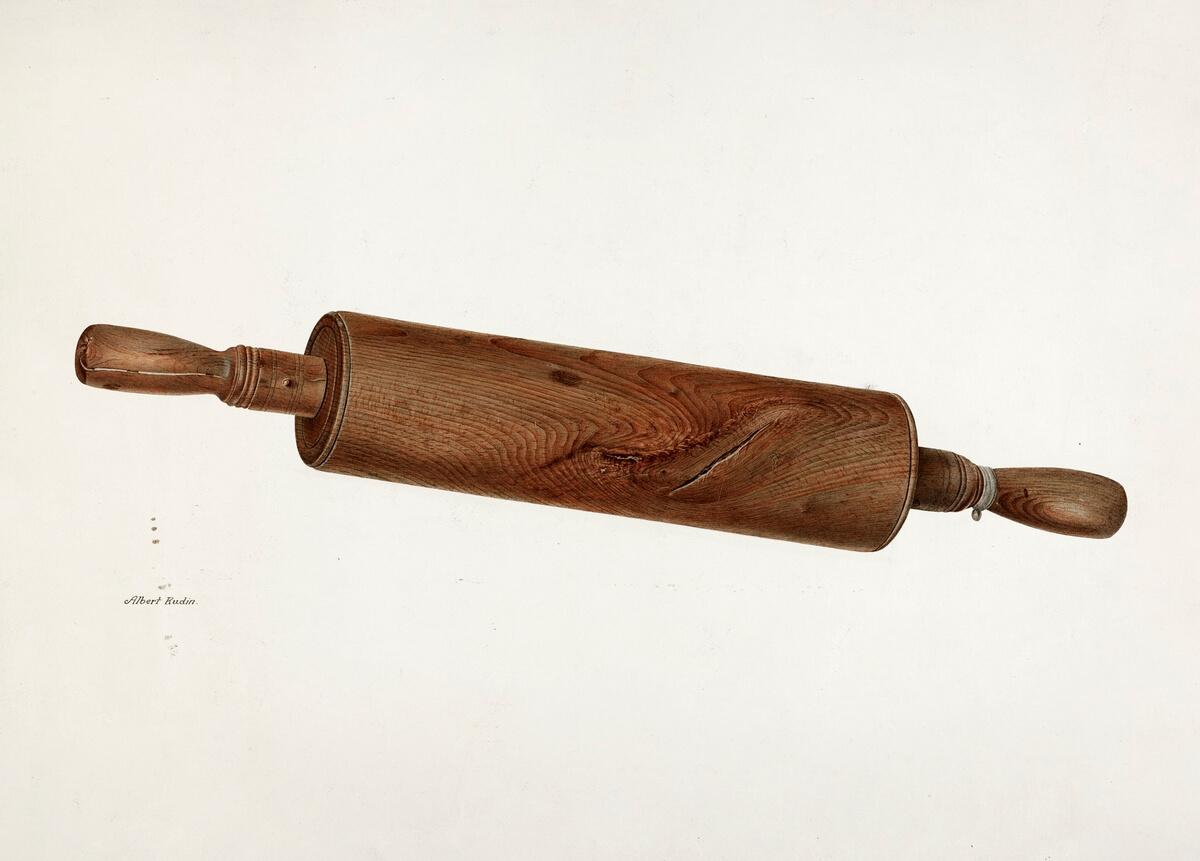
\includegraphics[width=1\linewidth]{imagenes/amasando}

Cómo ya hemos mencionado, es normal que la mayor parte del tiempo dedicado a un proyecto de análisis se nos vaya en la limpieza y orden de los datos disponibles. Aún cuando nuestros datos provengan de fuentes oficiales (un gobierno nacional, el Banco Mundial, etc) en muy rara ocasión podremos usarlos para nuestros fines sin antes procesarlos. Y aún si los datos llegaran en perfectas condiciones, no tenemos forma de saberlo hasta haber realizado una exploración para verificarlo.

Ésta inevitable etapa de preparación es llamada \emph{data wrangling} en inglés, algo así como el proceso de ``domar los datos''. El término hace referencia, en clave de humor, al esfuerzo que requiere la puesta en orden cuando los datos son cuantiosos, de muchas fuentes distintas, o en particular desprolijos. Para que la experiencia sea lo menos tediosa posible, y podamos pasar rápido al momento de extraer conocimiento, vamos a practicar algunas técnicas muy útiles de \emph{wrangling}.

\hypertarget{primeros-pasos-al-examinar-un-conjunto-de-datos-nuevo}{%
\section{Primeros pasos al examinar un conjunto de datos nuevo}\label{primeros-pasos-al-examinar-un-conjunto-de-datos-nuevo}}

Si no lo hicimos aún en la sesión en la que estamos trabajando, cargamos \texttt{tidyverse}.

\begin{Shaded}
\begin{Highlighting}[]
\FunctionTok{library}\NormalTok{(tidyverse)}
\end{Highlighting}
\end{Shaded}

Vamos a practicar usando el dataset de delitos que publica el Ministerio de Justicia y Seguridad de la Ciudad Autónoma de Buenos Aires. Registra los homicidios, hurtos (sin violencia), lesiones y robos (con violencia) ocurridos en la ciudad durante el año 2020. Vamos a trabajar con una versión de los datos que ha sido simplificada para hacer más ameno el trabajo con ella. Quién quiera acceder a los datos en su esplendor de complejidad original, puede encontrarlos en el portal de datos abiertos de la ciudad: \url{https://data.buenosaires.gob.ar/}.

Comenzamos por acceder al archivo con los registros para cargarlo en R como un dataframe. Esto requiere de una conexión a internet, pero no debería tomar mucho tiempo en ser descargado.

\begin{Shaded}
\begin{Highlighting}[]
\NormalTok{delitos }\OtherTok{\textless{}{-}} \FunctionTok{read.csv}\NormalTok{(}\StringTok{"https://cdaj.netlify.app/data/delitos\_barrios.csv"}\NormalTok{)}
\end{Highlighting}
\end{Shaded}

Lo primero que deberíamos hacer con un dataframe que no conocemos es usar la función \texttt{str()}, que nos indica su estructura (por \emph{structure} en inglés):

\begin{Shaded}
\begin{Highlighting}[]
\FunctionTok{str}\NormalTok{(delitos)}
\end{Highlighting}
\end{Shaded}

\begin{verbatim}
## 'data.frame':    3188 obs. of  5 variables:
##  $ periodo: chr  "01/2020" "01/2020" "01/2020" "01/2020" ...
##  $ tipo   : chr  "Homicidio" "Homicidio" "Homicidio" "Homicidio" ...
##  $ subtipo: chr  "Doloso" "Doloso" "Doloso" "Doloso" ...
##  $ barrio : chr  "Barracas" "Nueva Pompeya" "Retiro" "Saavedra" ...
##  $ total  : int  1 1 1 1 1 1 1 2 1 1 ...
\end{verbatim}

Para empezar, nos enteramos que el objeto que estamos analizando es un dataframe (``data.frame''). Eso ya lo sabíamos, pero como \texttt{str()} puede usarse con cualquier clase de objeto en R, en ocasiones resultará que estamos ante un vector, una lista u otra clase de criatura. A continuación aparecen las dimensiones del dataframe: 3188 observaciones (filas) con 5 variables (columnas). Los nombres de las columnas son \emph{periodo}, \emph{tipo}, \emph{subtipo}, \emph{barrio} y \emph{total}. Con eso ya podemos inferir que cada observación en el dataframe contiene la cantidad total de delitos según tipo y subtipo (aunque no sepamos bien de que se tratan esas variables), en un período dado y en cada barrio.

Con \texttt{str()} también obtenemos el tipo de datos representados por cada variable, y un ejemplo de los valores contenidos en las primeras filas. La variable \emph{total} es de tipo ``int'', es decir, números enteros o \emph{integers} en inglés. El resto de las variables son de tipo ``chr''; en R las variables de texto reciben el nombre de \emph{characters}, caracteres.

La siguiente función a utilizar cuando estamos conociendo el contenido de un set de datos es \texttt{summary()}, que nos dará un resumen en forma de estadísticas descriptivas para las variables numéricas (cuartiles y mediana) .

\begin{Shaded}
\begin{Highlighting}[]
\FunctionTok{summary}\NormalTok{(delitos)}
\end{Highlighting}
\end{Shaded}

\begin{verbatim}
##    periodo              tipo             subtipo             barrio         
##  Length:3188        Length:3188        Length:3188        Length:3188       
##  Class :character   Class :character   Class :character   Class :character  
##  Mode  :character   Mode  :character   Mode  :character   Mode  :character  
##                                                                             
##                                                                             
##                                                                             
##      total       
##  Min.   :  1.00  
##  1st Qu.:  3.00  
##  Median :  8.00  
##  Mean   : 20.93  
##  3rd Qu.: 22.00  
##  Max.   :393.00
\end{verbatim}

Para las variables de texto \texttt{summary()} no tiene mucho que decir. Aquí sería bueno que nos mostrara algún dato, quizás los valores más frecuentes, ¿verdad?. Eso va a ocurrir pero sólo cuando esas columnas con texto contengan variables categóricas, que en R reciben el tipo ``factor'' en lugar de ``chr''.

Una variable es categórica cuando es razonable considerar que se elige entre un conjunto finito de variables posibles; por ejemplo, los barrios de Buenos Aires son un conjunto finito y predeterminado.

¿Pero cómo puede saber R si \emph{tipo} o \emph{barrio} son categorías? Pues podemos avisarle al cargar los datos con la función \texttt{read.csv()} que usamos al principio. Para que \texttt{read.csv()} interprete como variables categóricas a todas las columnas que contienen texto se usa el parámetro \texttt{stringsAsFactors}, así: \texttt{misdatos\ \textless{}-\ read.csv("archivo\_con\_mis\_datos",\ stringsAsFactors\ =\ TRUE)}. En general es buena idea evitar que los campos de texto se asuman como factores, pero en éste caso está bien: aquí todas las columnas de texto, en efecto, contienen variables categóricas.

Veamos que pasa si lo intentamos. Volvemos a leer el mismo dataset, esta vez con \texttt{stringsAsFactors\ =\ TRUE}

\begin{Shaded}
\begin{Highlighting}[]
\NormalTok{delitos }\OtherTok{\textless{}{-}} \FunctionTok{read.csv}\NormalTok{(}\StringTok{"https://cdaj.netlify.app/data/delitos\_barrios.csv"}\NormalTok{, }\AttributeTok{stringsAsFactors =} \ConstantTok{TRUE}\NormalTok{)}
\end{Highlighting}
\end{Shaded}

.. y pedimos su resumen:

\begin{Shaded}
\begin{Highlighting}[]
\FunctionTok{summary}\NormalTok{(delitos)}
\end{Highlighting}
\end{Shaded}

\begin{verbatim}
##     periodo                        tipo                 subtipo    
##  01/2020: 284   Homicidio            : 163                  :1166  
##  02/2020: 281   Hurto (sin violencia):1087   Siniestro Vial : 644  
##  03/2020: 280   Lesiones             : 575   Con uso de moto: 517  
##  12/2020: 280   Robo (con violencia) :1363   Hurto Automotor: 504  
##  08/2020: 276                                Robo Automotor : 263  
##  11/2020: 274                                Doloso         :  81  
##  (Other):1513                                (Other)        :  13  
##            barrio         total       
##  Balvanera    :  81   Min.   :  1.00  
##  Barracas     :  81   1st Qu.:  3.00  
##  Flores       :  80   Median :  8.00  
##  Villa Lugano :  80   Mean   : 20.93  
##  Mataderos    :  76   3rd Qu.: 22.00  
##  Villa Soldati:  75   Max.   :393.00  
##  (Other)      :2715
\end{verbatim}

¡Esta vez obtuvimos un ranking con las categorías más frecuentes!

Las categorías posibles para un factor son llamadas ``niveles'' (\emph{levels}). Para ver todos los niveles del factor \emph{barrio}, es decir todos los barrios representados en la columna con ese nombre de variable, podemos usar la función \texttt{levels()}

\begin{Shaded}
\begin{Highlighting}[]
\FunctionTok{levels}\NormalTok{(delitos}\SpecialCharTok{$}\NormalTok{barrio)}
\end{Highlighting}
\end{Shaded}

\begin{verbatim}
##  [1] ""                  "Agronomía"         "Almagro"          
##  [4] "Balvanera"         "Barracas"          "Belgrano"         
##  [7] "Boca"              "Boedo"             "Caballito"        
## [10] "Chacarita"         "Coghlan"           "Colegiales"       
## [13] "Constitución"      "Flores"            "Floresta"         
## [16] "La Boca"           "Liniers"           "Mataderos"        
## [19] "Monserrat"         "Monte Castro"      "Nueva Pompeya"    
## [22] "Nuñez"             "Palermo"           "Parque Avellaneda"
## [25] "Parque Chacabuco"  "Parque Chas"       "Parque Patricios" 
## [28] "Paternal"          "Puerto Madero"     "Recoleta"         
## [31] "Retiro"            "Saavedra"          "San Cristóbal"    
## [34] "San Nicolás"       "San Telmo"         "Vélez Sársfield"  
## [37] "Versalles"         "Villa Crespo"      "Villa Del Parque" 
## [40] "Villa Devoto"      "Villa Gral. Mitre" "Villa Lugano"     
## [43] "Villa Luro"        "Villa Ortuzar"     "Villa Pueyrredón" 
## [46] "Villa Real"        "Villa Riachuelo"   "Villa Santa Rita" 
## [49] "Villa Soldati"     "Villa Urquiza"
\end{verbatim}

Para acceder en forma rápida al contenido de la columna \emph{barrio}, hemos utilizado por primera vez un truco muy práctico. Para obtener el contenido de cualquier columna en particular, basta con el nombre del dataframe seguido del símbolo \texttt{\$} y el nombre de la columna a extraer: \texttt{delitos\$tipo}, o \texttt{delitos\$total}, etc.

\hypertarget{cruzando-variables-la-operaciuxf3n-join}{%
\section{\texorpdfstring{Cruzando variables: la operación \texttt{join}}{Cruzando variables: la operación join}}\label{cruzando-variables-la-operaciuxf3n-join}}

Al realizar un análisis ``en la vida real'', es decir, usando datos salvajes en lugar de los prolijos datasets de práctica, es muy habitual encontrar que nos falta una variable que necesitamos. Si tenemos suerte, la información que necesitamos también está disponible en forma de tabla, con algún campo en común, y podemos llevar el cabo un cruce de datos para traérnosla.

Para expresarlo con un ejemplo concreto: hemos visto que los registros de delitos incluyen una columna con el barrio, que es la única variable relacionada con la geografía. Si nuestra unidad de análisis fuera la comuna\footnote{La Ciudad de Buenos Aires se encuentra organizada en 15 Comunas. Son unidades descentralizadas de gestión política y administrativa que, en general, abarcan varios barrios.} en lugar del barrio, necesitaríamos agregar la columna correspondiente. En este caso, estamos de suerte porque una tabla con los barrios de la Ciudad de Buenos Aires y la comuna a la que pertenecen es fácil de conseguir. Con esa tabla en nuestro poder, ya tenemos las piezas necesarias para el cruce de datos. En cada registro en el dataframe de delitos tenemos un barrio; podemos buscarlo en la tabla de barrios y comunas, tomar nota de la comuna asociada, y copiarla en nuestro dataset original. Por supuesto, hacerlo a mano para cada uno de las miles de filas en nuestro dataframe tardaría una eternidad, amén de que quizás podríamos hartarnos de la tarea antes de terminar. ¡Nada de eso! Vamos a resolverlo en meros instantes escribiendo unas pocas líneas de código. Antes de continuar hagamos una pausa para conmiserar a los investigadores de eras pasadas, antes de la popularización de la computadora personal, que realizaban tareas de esta escala con lápiz, papel y paciencia.

Existe una gran variedad de funciones que permiten combinar tablas relacionadas entre sí por una o varias variables en común. Para nuestro propósito, alcanza con conocer una: \texttt{left\_join()}. La función toma como parámetros dos dataframes (que son tablas al fin y al cabo) busca las variables que tengan el mismo nombre y usándolas como referencia completa la primera de ellas, la de la izquierda, con los datos nuevos que aporta la segunda. \texttt{left\_join} devuelve un dataframe nuevo con los datos combinados.

Manos a la obra. Descargamos el dataframe con barrios y comunas:

\begin{Shaded}
\begin{Highlighting}[]
\NormalTok{barrios\_comunas }\OtherTok{\textless{}{-}} \FunctionTok{read.csv}\NormalTok{(}\StringTok{"https://cdaj.netlify.app/data/barrios\_comunas.csv"}\NormalTok{)}
\end{Highlighting}
\end{Shaded}

Si recibimos un mensaje de error al estilo de \textbf{\texttt{{[}...{]}\ Error\ in\ left\_join(delitos,\ barrios\_comunas)\ :\ \ \ \ could\ not\ find\ function\ "left\_join"}} es muy probable que nos hayamos olvidado de activar las funciones de Tidyverse. En ese caso, sólo necesitamos ejecutar \texttt{library(tidyverse)} e intentar de nuevo.

Echamos un vistazo, comprobando que existe ``barrios'', una columna en común que lo relaciona con el dataframe de delitos,

\begin{Shaded}
\begin{Highlighting}[]
\NormalTok{barrios\_comunas}
\end{Highlighting}
\end{Shaded}

\begin{verbatim}
##               barrio comuna
## 1          Agronomía     15
## 2            Almagro      5
## 3          Balvanera      3
## 4           Barracas      4
## 5           Belgrano     13
## 6               Boca      4
## 7              Boedo      5
## 8          Caballito      6
## 9          Chacarita     15
## 10           Coghlan     12
## 11        Colegiales     13
## 12      Constitución      1
## 13            Flores      7
## 14          Floresta     10
## 15           La Boca      4
## 16           Liniers      9
## 17         Mataderos      9
## 18         Monserrat      1
## 19      Monte Castro     10
## 20     Nueva Pompeya      4
## 21             Nuñez     13
## 22           Palermo     14
## 23 Parque Avellaneda      9
## 24  Parque Chacabuco      7
## 25       Parque Chas     15
## 26  Parque Patricios      4
## 27          Paternal     15
## 28     Puerto Madero      1
## 29          Recoleta      2
## 30            Retiro      1
## 31          Saavedra     12
## 32     San Cristóbal      3
## 33       San Nicolás      1
## 34         San Telmo      1
## 35   Vélez Sársfield     10
## 36         Versalles     10
## 37      Villa Crespo     15
## 38  Villa Del Parque     11
## 39      Villa Devoto     11
## 40 Villa Gral. Mitre     11
## 41      Villa Lugano      8
## 42        Villa Luro     10
## 43     Villa Ortuzar     15
## 44  Villa Pueyrredón     12
## 45        Villa Real     10
## 46   Villa Riachuelo      8
## 47  Villa Santa Rita     11
## 48     Villa Soldati      8
## 49     Villa Urquiza     12
\end{verbatim}

y lo unimos (de allí el término ``join'', unir en inglés) a nuestra data:

\begin{Shaded}
\begin{Highlighting}[]
\NormalTok{delitos }\OtherTok{\textless{}{-}} \FunctionTok{left\_join}\NormalTok{(delitos, barrios\_comunas)}
\end{Highlighting}
\end{Shaded}

Admiremos nuestra obra:

\begin{Shaded}
\begin{Highlighting}[]
\FunctionTok{head}\NormalTok{(delitos)}
\end{Highlighting}
\end{Shaded}

\begin{verbatim}
##   periodo      tipo        subtipo        barrio total comuna
## 1 01/2020 Homicidio         Doloso      Barracas     1      4
## 2 01/2020 Homicidio         Doloso Nueva Pompeya     1      4
## 3 01/2020 Homicidio         Doloso        Retiro     1      1
## 4 01/2020 Homicidio         Doloso      Saavedra     1     12
## 5 01/2020 Homicidio      Femicidio  Villa Devoto     1     11
## 6 01/2020 Homicidio Siniestro Vial     Balvanera     1      3
\end{verbatim}

Es así de fácil. Bueno, no tanto\ldots{} este fue un caso sencillo, pero hay todo tipo de datos y cruces allí afuera, y a veces se necesitan operaciones más complejas. Por eso hay toda una familia de funciones de \emph{join} - \texttt{right\_join()}, \texttt{inner\_join()}, \texttt{full\_join}, \texttt{anti\_join()}, y alguna más. Pero podemos dejarlas en paz; para nuestras necesidades, con \texttt{left\_join()} podemos arreglarnos muy bien.

Satisfechos con la mejora, si queremos guardar el dataframe ``mejorado'' para usarlo en otra ocasión, podemos hacerlo con \texttt{write.csv()}, que lo convierte en un archivo de texto que queda en nuestra PC.

\begin{Shaded}
\begin{Highlighting}[]
\FunctionTok{write.csv}\NormalTok{(delitos, }\StringTok{"delitos.csv"}\NormalTok{, }\AttributeTok{row.names =} \ConstantTok{FALSE}\NormalTok{)}
\end{Highlighting}
\end{Shaded}

Podemos seguir siempre ese formato para guardar nuestros datos. El primer parámetro es el dataframe que vamos a guardar, el segundo -siempre entre comillas- es el nombre de archivo, y la opción final, \texttt{row.names\ =\ FALSE} sirve para evitar que R le agregue una columna al principio con números consecutivos (1, 2, 3, y así), cosa que quizás fue útil alguna vez pero en general no necesitamos.

Para volver a leer los datos en otra ocasión, usamos \texttt{read.csv()} tal como ya hemos hecho.

\begin{Shaded}
\begin{Highlighting}[]
\NormalTok{delitos }\OtherTok{\textless{}{-}} \FunctionTok{read.csv}\NormalTok{(}\StringTok{"delitos.csv"}\NormalTok{)}
\end{Highlighting}
\end{Shaded}

Y si queremos saber exactamente dónde ha guardado R nuestros datos, por ejemplo para abrirlos con otro programa, usamos la función \texttt{getwd} (por \emph{get working directory} )

\begin{Shaded}
\begin{Highlighting}[]
\FunctionTok{getwd}\NormalTok{()}
\end{Highlighting}
\end{Shaded}

El resultado será la dirección (la ubicación de la la carpeta), donde estamos trabajando y hemos guardado los datos; por ejemplo \texttt{/home/antonio/Practicando\ R/}.

\hypertarget{transformando-los-datos}{%
\section{Transformando los datos}\label{transformando-los-datos}}

Habiendo revisado el contenido de un dataframe (y agregado alguna variable si hiciera falta), comenzamos a hacernos idea de los ajustes que necesita para que los datos tomen el formato que necesitamos. Estos ajustes pueden ser correcciones (por ejemplo, de errores de tipeo cuando se cargaron los datos), la creación de nuevas variables derivadas de las existentes, o un reordenamiento de los datos para simplificar nuestro trabajo.

Para hacer todo esto, y mucho más, vamos a aprender funciones que representan cinco verbos básicos para la transformación de datos:

\begin{itemize}
\tightlist
\item
  \texttt{select()}: seleccionar -elegir- columnas por su nombre
\item
  \texttt{filter()}: filtrar, es decir quedarse sólo con las filas que cumplan cierta condición
\item
  \texttt{arrange()}: ordenar las filas de acuerdo a su contenido o algún otro índice
\item
  \texttt{mutate()}: mutar -cambiar- un dataframe, modificando el contenido de sus columnas o creando columnas (es decir, variables) nuevas
\item
  \texttt{summarise()}: producir sumarios -un valor extraído de muchos, por ejemplo el promedio- con el contenido de las columnas
\end{itemize}

Estas funciones tienen una sintaxis, una forma de escribirse, uniforme. El primer argumento que toman siempre es un dataframe; los siguientes indican qué hacer con los datos. El resultado siempre es un nuevo dataframe.

Las funciones son parte de \href{http://dplyr.tidyverse.org/}{dplyr}, uno de los componentes de la familia de paquetes \href{https://www.tidyverse.org/}{Tidyverse}. Ya tenemos disponible todo lo necesario, activado cuando invocamos \texttt{library(tidyverse)} al comienzo.

Manos a la obra.

\hypertarget{seleccionar-columnas-con-select}{%
\subsection{\texorpdfstring{Seleccionar columnas con \texttt{select()}}{Seleccionar columnas con select()}}\label{seleccionar-columnas-con-select}}

Muchas veces tendremos que lidiar con datasets con decenas de variables. Alguna que otra vez, con centenas. En esos casos el primer problema es librarnos de semejante cantidad de columnas, reteniendo sólo aquellas en las que estamos interesados. Para un dataset como el de reclamos de los ciudadanos, que tiene pocas columnas, select() no es tan importante. Aún así, podemos usar select() con fines demostrativos.

Sabemos que el dataset tiene 6 columnas:

\begin{Shaded}
\begin{Highlighting}[]
\FunctionTok{names}\NormalTok{(delitos)}
\end{Highlighting}
\end{Shaded}

\begin{verbatim}
## [1] "periodo" "tipo"    "subtipo" "barrio"  "total"   "comuna"
\end{verbatim}

Si quisiéramos sólo las que contienen el período y el total, las seleccionamos por nombre, a continuación del nombre del dataframe:

\begin{Shaded}
\begin{Highlighting}[]
\NormalTok{seleccion }\OtherTok{\textless{}{-}} \FunctionTok{select}\NormalTok{(delitos, periodo, total)}

\FunctionTok{head}\NormalTok{(seleccion)}
\end{Highlighting}
\end{Shaded}

\begin{verbatim}
##   periodo total
## 1 01/2020     1
## 2 01/2020     1
## 3 01/2020     1
## 4 01/2020     1
## 5 01/2020     1
## 6 01/2020     1
\end{verbatim}

También podemos seleccionar por contigüidad, por ejemplo ``todas las columnas que van de \emph{tipo} a \emph{barrio}'':

\begin{Shaded}
\begin{Highlighting}[]
\NormalTok{seleccion }\OtherTok{\textless{}{-}} \FunctionTok{select}\NormalTok{(delitos, tipo}\SpecialCharTok{:}\NormalTok{barrio)}

\FunctionTok{head}\NormalTok{(seleccion)}
\end{Highlighting}
\end{Shaded}

\begin{verbatim}
##        tipo        subtipo        barrio
## 1 Homicidio         Doloso      Barracas
## 2 Homicidio         Doloso Nueva Pompeya
## 3 Homicidio         Doloso        Retiro
## 4 Homicidio         Doloso      Saavedra
## 5 Homicidio      Femicidio  Villa Devoto
## 6 Homicidio Siniestro Vial     Balvanera
\end{verbatim}

Y podemos seleccionar por omisión. Si nos interesara todo el contenido del dataset menos la variable \emph{subtipo}, usaríamos

\begin{Shaded}
\begin{Highlighting}[]
\NormalTok{seleccion }\OtherTok{\textless{}{-}} \FunctionTok{select}\NormalTok{(delitos, }\SpecialCharTok{{-}}\NormalTok{subtipo)}

\FunctionTok{head}\NormalTok{(seleccion)}
\end{Highlighting}
\end{Shaded}

\begin{verbatim}
##   periodo      tipo        barrio total comuna
## 1 01/2020 Homicidio      Barracas     1      4
## 2 01/2020 Homicidio Nueva Pompeya     1      4
## 3 01/2020 Homicidio        Retiro     1      1
## 4 01/2020 Homicidio      Saavedra     1     12
## 5 01/2020 Homicidio  Villa Devoto     1     11
## 6 01/2020 Homicidio     Balvanera     1      3
\end{verbatim}

Al igual que con las selección por inclusión, podemos seleccionar por omisión de un rango de columnas contiguas (escritas entre paréntesis), o de varias columnas nombradas:

\begin{Shaded}
\begin{Highlighting}[]
\NormalTok{seleccion }\OtherTok{\textless{}{-}} \FunctionTok{select}\NormalTok{(delitos, }\SpecialCharTok{{-}}\NormalTok{(subtipo}\SpecialCharTok{:}\NormalTok{total))}

\FunctionTok{head}\NormalTok{(seleccion)}
\end{Highlighting}
\end{Shaded}

\begin{verbatim}
##   periodo      tipo comuna
## 1 01/2020 Homicidio      4
## 2 01/2020 Homicidio      4
## 3 01/2020 Homicidio      1
## 4 01/2020 Homicidio     12
## 5 01/2020 Homicidio     11
## 6 01/2020 Homicidio      3
\end{verbatim}

\begin{Shaded}
\begin{Highlighting}[]
\NormalTok{seleccion }\OtherTok{\textless{}{-}} \FunctionTok{select}\NormalTok{(delitos, }\SpecialCharTok{{-}}\NormalTok{tipo, }\SpecialCharTok{{-}}\NormalTok{barrio)}

\FunctionTok{head}\NormalTok{(seleccion)}
\end{Highlighting}
\end{Shaded}

\begin{verbatim}
##   periodo        subtipo total comuna
## 1 01/2020         Doloso     1      4
## 2 01/2020         Doloso     1      4
## 3 01/2020         Doloso     1      1
## 4 01/2020         Doloso     1     12
## 5 01/2020      Femicidio     1     11
## 6 01/2020 Siniestro Vial     1      3
\end{verbatim}

\hypertarget{filtrar-filas-con-filter}{%
\subsection{\texorpdfstring{Filtrar filas con \texttt{filter()}}{Filtrar filas con filter()}}\label{filtrar-filas-con-filter}}

Una de las tareas más frecuentes en el análisis de datos es la de identificar observaciones que cumplen con determinada condición. \texttt{filter()} permite extraer subconjuntos del total en base a sus variables.

Por ejemplo, para seleccionar registros que correspondan a Retiro, ocurridos en el primer mes de 2020 (período ``01/2020''):

\begin{Shaded}
\begin{Highlighting}[]
\NormalTok{seleccion }\OtherTok{\textless{}{-}} \FunctionTok{filter}\NormalTok{(delitos, barrio }\SpecialCharTok{==} \StringTok{"Retiro"}\NormalTok{, periodo }\SpecialCharTok{==} \StringTok{"01/2020"}\NormalTok{)}
\FunctionTok{head}\NormalTok{(seleccion)}
\end{Highlighting}
\end{Shaded}

\begin{verbatim}
##   periodo                  tipo         subtipo barrio total comuna
## 1 01/2020             Homicidio          Doloso Retiro     1      1
## 2 01/2020 Hurto (sin violencia)                 Retiro   130      1
## 3 01/2020 Hurto (sin violencia) Hurto Automotor Retiro     2      1
## 4 01/2020              Lesiones  Siniestro Vial Retiro    16      1
## 5 01/2020  Robo (con violencia)                 Retiro   165      1
## 6 01/2020  Robo (con violencia) Con uso de moto Retiro    12      1
\end{verbatim}

\hypertarget{comparaciones}{%
\subsubsection{Comparaciones}\label{comparaciones}}

Aquí hemos usado un recurso nuevo, la comparación. R provee una serie de símbolos que permite comparar valores entre sí:

\begin{itemize}
\item
  \texttt{==} igual a
\item
  \texttt{!=} no igual (distinto) a
\item
  \texttt{\textgreater{}} mayor a
\item
  \texttt{\textgreater{}=} mayor o igual a
\item
  \texttt{\textless{}} menor a
\item
  \texttt{\textless{}=} menor o igual a
\end{itemize}

Atención especial merece el símbolo que compara igualdad, \texttt{==}. Un error muy común es escribir \texttt{barrio\ =\ "Retiro"}, (un sólo símbolo \texttt{=}) que le indica a R que guarde el valor ``Retiro'' dentro de la variable \emph{barrio}, en lugar de verificar si son iguales. Para ésto último, lo correcto es \texttt{barrio\ ==\ "Retiro"}, tal como lo usamos en el ejemplo para \texttt{filter()}.

También hay que tener en cuenta el uso de comillas. Para que R no se confunda, cuando queramos usar valores de texto (de tipo \emph{character}) los rodeamos con comillas para que quede claro que no nos referimos a una variable con ese nombre, si la hubiera, sino en forma literal a esa palabra o secuencia de texto. En el caso de los números, no hace falta el uso de comillas, ya que en R ningún nombre de variable puede comenzar con o estar compuesta sólo por números.

Filtrando los registros de períodos para los cuales se registran más de 100 incidentes:

\begin{Shaded}
\begin{Highlighting}[]
\NormalTok{seleccion }\OtherTok{\textless{}{-}} \FunctionTok{filter}\NormalTok{(delitos, total }\SpecialCharTok{\textgreater{}} \DecValTok{100}\NormalTok{)}
\FunctionTok{head}\NormalTok{(seleccion)}
\end{Highlighting}
\end{Shaded}

\begin{verbatim}
##   periodo                  tipo subtipo    barrio total comuna
## 1 01/2020 Hurto (sin violencia)           Almagro   142      5
## 2 01/2020 Hurto (sin violencia)         Balvanera   306      3
## 3 01/2020 Hurto (sin violencia)          Belgrano   142     13
## 4 01/2020 Hurto (sin violencia)         Caballito   157      6
## 5 01/2020 Hurto (sin violencia)            Flores   143      7
## 6 01/2020 Hurto (sin violencia)         Monserrat   127      1
\end{verbatim}

\hypertarget{operadores-luxf3gicos}{%
\subsubsection{Operadores lógicos}\label{operadores-luxf3gicos}}

Cuando le pasamos múltiples condiciones a filter(), la función devuelve las filas que cumplen con todas.

Por ejemplo, con

\begin{Shaded}
\begin{Highlighting}[]
\NormalTok{seleccion }\OtherTok{\textless{}{-}} \FunctionTok{filter}\NormalTok{(delitos, periodo }\SpecialCharTok{==} \StringTok{"08/2020"}\NormalTok{,  tipo }\SpecialCharTok{==} \StringTok{"Homicidio"}\NormalTok{)}

\FunctionTok{head}\NormalTok{(seleccion)}
\end{Highlighting}
\end{Shaded}

\begin{verbatim}
##   periodo      tipo subtipo       barrio total comuna
## 1 08/2020 Homicidio  Doloso     Barracas     4      4
## 2 08/2020 Homicidio  Doloso     Belgrano     1     13
## 3 08/2020 Homicidio  Doloso         Boca     1      4
## 4 08/2020 Homicidio  Doloso    Caballito     1      6
## 5 08/2020 Homicidio  Doloso    Chacarita     3     15
## 6 08/2020 Homicidio  Doloso Constitución     1      1
\end{verbatim}

obtenemos todos los registros cuyo rubro es ``Homicidio'', y cuyo período es 08/2020, agosto de 2020.

Siguiendo el mismo formato, si intentamos

\begin{Shaded}
\begin{Highlighting}[]
\NormalTok{seleccion }\OtherTok{\textless{}{-}} \FunctionTok{filter}\NormalTok{(delitos, barrio }\SpecialCharTok{==} \StringTok{"Retiro"}\NormalTok{, barrio }\SpecialCharTok{==} \StringTok{"Palermo"}\NormalTok{)}

\FunctionTok{head}\NormalTok{(seleccion)}
\end{Highlighting}
\end{Shaded}

\begin{verbatim}
## [1] periodo tipo    subtipo barrio  total   comuna 
## <0 rows> (or 0-length row.names)
\end{verbatim}

obtenemos un conjunto vacío. ¿Por qué? Es debido a que ninguna observación cumple con todas las condiciones; en ningún registro el barrio es Retiro y también es Palermo. ¡Suena razonable!. Para obtener registros ocurridos en Retiro \textbf{ó} en Palermo, usamos el operador lógico \texttt{\textbar{}} que significa\ldots{} ``ó''.

\begin{Shaded}
\begin{Highlighting}[]
\NormalTok{seleccion }\OtherTok{\textless{}{-}} \FunctionTok{filter}\NormalTok{(delitos, barrio }\SpecialCharTok{==} \StringTok{"Retiro"} \SpecialCharTok{|}\NormalTok{ barrio }\SpecialCharTok{==} \StringTok{"Palermo"}\NormalTok{)}

\FunctionTok{head}\NormalTok{(seleccion)}
\end{Highlighting}
\end{Shaded}

\begin{verbatim}
##   periodo                  tipo         subtipo  barrio total comuna
## 1 01/2020             Homicidio          Doloso  Retiro     1      1
## 2 01/2020 Hurto (sin violencia)                 Palermo   349     14
## 3 01/2020 Hurto (sin violencia)                  Retiro   130      1
## 4 01/2020 Hurto (sin violencia) Hurto Automotor Palermo    19     14
## 5 01/2020 Hurto (sin violencia) Hurto Automotor  Retiro     2      1
## 6 01/2020              Lesiones  Siniestro Vial Palermo    48     14
\end{verbatim}

Se trata de la lógica de conjuntos, o lógica \emph{booleana}, que con un poco de suerte recordamos de nuestra época de escolares. Los símbolos importantes son \texttt{\&}, \texttt{\textbar{}}, y \texttt{!}: ``y'', ``ó'', y la negación que invierte preposiciones:

\begin{itemize}
\item
  \texttt{a\ \&\ b} a y b
\item
  \texttt{a\ \textbar{}\ b} a ó b
\item
  \texttt{a\ \&\ !b} a, y no b
\item
  \texttt{!a\ \&\ b} no a, y b
\item
  \texttt{!(a\ \&\ b)} no (a y b)
\end{itemize}

Hemos visto ejemplos de \texttt{a\ \&\ b} (\texttt{periodo\ ==\ "08/2020",\ \ tipo\ ==\ "Homicidio"}, que \texttt{filter()} toma como un \texttt{\&}) y de \texttt{a\ \textbar{}\ b} (cuando optamos por \texttt{barrio\ ==\ "Retiro"\ \textbar{}\ barrio\ ==\ "Palermo"})

Un ejemplo de \texttt{a\ \&\ !b} : pedimos filas en las que el tipo sea ``Robo (con violencia)'', y además el subtipo no sea ``Robo Automotor'':

\begin{Shaded}
\begin{Highlighting}[]
\FunctionTok{filter}\NormalTok{(delitos, tipo }\SpecialCharTok{==} \StringTok{"Robo (con violencia)"} \SpecialCharTok{\&} \SpecialCharTok{!}\NormalTok{(subtipo }\SpecialCharTok{==} \StringTok{"Robo Automotor"}\NormalTok{))}
\end{Highlighting}
\end{Shaded}

Y como ejemplo de \texttt{!(a\ \&\ b)}, todas las filas excepto las de tipo ``Homicidio'' con subtipo ``Siniestro Vial'':

\begin{Shaded}
\begin{Highlighting}[]
\NormalTok{seleccion }\OtherTok{\textless{}{-}} \FunctionTok{filter}\NormalTok{(delitos, }\SpecialCharTok{!}\NormalTok{(tipo }\SpecialCharTok{==} \StringTok{"Homicidio"} \SpecialCharTok{\&}\NormalTok{ subtipo }\SpecialCharTok{==} \StringTok{"Siniestro Vial"}\NormalTok{))}

\FunctionTok{head}\NormalTok{(seleccion)}
\end{Highlighting}
\end{Shaded}

\begin{verbatim}
##   periodo                  tipo   subtipo        barrio total comuna
## 1 01/2020             Homicidio    Doloso      Barracas     1      4
## 2 01/2020             Homicidio    Doloso Nueva Pompeya     1      4
## 3 01/2020             Homicidio    Doloso        Retiro     1      1
## 4 01/2020             Homicidio    Doloso      Saavedra     1     12
## 5 01/2020             Homicidio Femicidio  Villa Devoto     1     11
## 6 01/2020 Hurto (sin violencia)                             5     NA
\end{verbatim}

\hypertarget{ordenar-filas-con-arrange}{%
\subsection{\texorpdfstring{Ordenar filas con \texttt{arrange()}}{Ordenar filas con arrange()}}\label{ordenar-filas-con-arrange}}

La función \texttt{arrange()} cambia el orden en el que aparecen las filas de un dataframe. Como primer parámetro toma un dataframe, al igual que el resto de los verbos de transformación que estamos aprendiendo. A continuación, espera un set de columnas para definir el orden.

Por ejemplo, para ordenar por total de registros:

\begin{Shaded}
\begin{Highlighting}[]
\NormalTok{ordenado }\OtherTok{\textless{}{-}} \FunctionTok{arrange}\NormalTok{(delitos, total)}

\FunctionTok{head}\NormalTok{(ordenado)}
\end{Highlighting}
\end{Shaded}

\begin{verbatim}
##   periodo      tipo        subtipo        barrio total comuna
## 1 01/2020 Homicidio         Doloso      Barracas     1      4
## 2 01/2020 Homicidio         Doloso Nueva Pompeya     1      4
## 3 01/2020 Homicidio         Doloso        Retiro     1      1
## 4 01/2020 Homicidio         Doloso      Saavedra     1     12
## 5 01/2020 Homicidio      Femicidio  Villa Devoto     1     11
## 6 01/2020 Homicidio Siniestro Vial     Balvanera     1      3
\end{verbatim}

Si agregamos más columnas, se usan en orden para ``desempatar''. Por ejemplo, si queremos que las filas con el mismo valor en \emph{total} aparezcan en el orden alfabético del barrio que les corresponde, sólo necesitamos agregar esa columna:

\begin{Shaded}
\begin{Highlighting}[]
\NormalTok{ordenado }\OtherTok{\textless{}{-}} \FunctionTok{arrange}\NormalTok{(delitos, total, barrio)}

\FunctionTok{head}\NormalTok{(ordenado)}
\end{Highlighting}
\end{Shaded}

\begin{verbatim}
##   periodo                  tipo         subtipo    barrio total comuna
## 1 05/2020  Robo (con violencia) Con uso de moto               1     NA
## 2 09/2020  Robo (con violencia)                               1     NA
## 3 12/2020  Robo (con violencia)  Robo Automotor               1     NA
## 4 03/2020              Lesiones  Siniestro Vial Agronomía     1     15
## 5 04/2020              Lesiones  Siniestro Vial Agronomía     1     15
## 6 06/2020 Hurto (sin violencia) Hurto Automotor Agronomía     1     15
\end{verbatim}

Si no se aclara lo contrario, el orden siempre es ascendente (de menor a mayor). Si quisiéramos orden de mayor a menor, usamos \texttt{desc()}:

\begin{Shaded}
\begin{Highlighting}[]
\NormalTok{ordenado }\OtherTok{\textless{}{-}} \FunctionTok{arrange}\NormalTok{(delitos, }\FunctionTok{desc}\NormalTok{(total))}

\FunctionTok{head}\NormalTok{(ordenado)}
\end{Highlighting}
\end{Shaded}

\begin{verbatim}
##   periodo                  tipo subtipo    barrio total comuna
## 1 02/2020 Hurto (sin violencia)           Palermo   393     14
## 2 01/2020  Robo (con violencia)           Palermo   362     14
## 3 02/2020  Robo (con violencia)           Palermo   356     14
## 4 01/2020 Hurto (sin violencia)           Palermo   349     14
## 5 01/2020  Robo (con violencia)         Balvanera   323      3
## 6 01/2020 Hurto (sin violencia)         Balvanera   306      3
\end{verbatim}

\hypertarget{valores-faltantes}{%
\subsubsection{Valores faltantes}\label{valores-faltantes}}

En el último ejemplo, aparecen varias filas cuyo valor para la columna BARRIO es \texttt{NA}. R representa los valores ausentes, desconocidos, con \texttt{NA} (``no disponible'', del inglés \emph{Not Available}). Hay que tener cuidado con los valores \texttt{NA}, porque la mayoría de las comparaciones y operaciones lógicas que los involucran resultan indefinidas. En la práctica:

¿Es 10 mayor a un valor desconocido?

\begin{Shaded}
\begin{Highlighting}[]
\DecValTok{10} \SpecialCharTok{\textgreater{}} \ConstantTok{NA}
\end{Highlighting}
\end{Shaded}

\begin{verbatim}
## [1] NA
\end{verbatim}

R no sabe. (Nadie lo sabe, para ser justos)

¿A cuanto asciende la suma de 10 más un valor desconocido?

\begin{Shaded}
\begin{Highlighting}[]
\ConstantTok{NA} \SpecialCharTok{+} \DecValTok{10}
\end{Highlighting}
\end{Shaded}

\begin{verbatim}
## [1] NA
\end{verbatim}

Y en particular\ldots{} ¿es un valor desconocido igual a otro valor desconocido?

\begin{Shaded}
\begin{Highlighting}[]
\ConstantTok{NA} \SpecialCharTok{==} \ConstantTok{NA}
\end{Highlighting}
\end{Shaded}

\begin{verbatim}
## [1] NA
\end{verbatim}

Por supuesto, la respuesta es desconocida también. La insistencia de R en no definir operaciones que involucran NA's podría parecer irritante a primera vista, pero en realidad nos hace un favor. Al evitar extraer conclusiones cuando trata con datos faltantes, nos evita caer en errores garrafales en los casos en que analizamos y comparamos datos incompletos. Además, podemos preguntar a R si un valor es desconocido, y allí si contesta con seguridad. La función requerida es \texttt{is.na()}.

\begin{Shaded}
\begin{Highlighting}[]
\NormalTok{desconocido }\OtherTok{\textless{}{-}} \ConstantTok{NA}

\FunctionTok{is.na}\NormalTok{(desconocido)}
\end{Highlighting}
\end{Shaded}

\begin{verbatim}
## [1] TRUE
\end{verbatim}

Algo más a tener en cuenta con los valores desconocidos es cómo son interpretados cuando usamos funciones de transformación de datos. Por ejemplo, \texttt{filter()} ignora las filas que contienen NA's en la variable que usa para filtrar. \texttt{arrange()} muestra las filas con NA's en el campo por el que ordena, pero todas al final.

\hypertarget{agregar-nuevas-variables-con-mutate}{%
\subsection{\texorpdfstring{Agregar nuevas variables con \texttt{mutate()}}{Agregar nuevas variables con mutate()}}\label{agregar-nuevas-variables-con-mutate}}

Recurrimos a la función \texttt{mutate()} cuando queremos agregarle columnas adicionales a nuestro dataframe, en general en base a los valores de las columnas ya existentes. Vamos a ilustrarlo con un ejemplo sencillo. Imaginemos que tenemos el siguiente dataset:

\begin{Shaded}
\begin{Highlighting}[]
\NormalTok{circulos }\OtherTok{\textless{}{-}} \FunctionTok{data.frame}\NormalTok{(}\AttributeTok{nombre =} \FunctionTok{c}\NormalTok{(}\StringTok{"Círculo 1"}\NormalTok{, }\StringTok{"Círculo 2"}\NormalTok{, }\StringTok{"Círculo 3"}\NormalTok{),}
\NormalTok{                       tamaño }\OtherTok{=} \FunctionTok{c}\NormalTok{(}\StringTok{"Pequeño"}\NormalTok{, }\StringTok{"Mediano"}\NormalTok{, }\StringTok{"Grande"}\NormalTok{),}
                       \AttributeTok{radio  =} \FunctionTok{c}\NormalTok{(}\DecValTok{1}\NormalTok{, }\DecValTok{3}\NormalTok{, }\DecValTok{5}\NormalTok{))}

\NormalTok{circulos}
\end{Highlighting}
\end{Shaded}

\begin{verbatim}
##      nombre  tamaño radio
## 1 Círculo 1 Pequeño     1
## 2 Círculo 2 Mediano     3
## 3 Círculo 3  Grande     5
\end{verbatim}

Podemos agregar una columna con el área de cada círculo con mutate():

\begin{Shaded}
\begin{Highlighting}[]
\FunctionTok{mutate}\NormalTok{(circulos, }\AttributeTok{area =} \FloatTok{3.1416} \SpecialCharTok{*}\NormalTok{ radio}\SpecialCharTok{\^{}}\DecValTok{2}\NormalTok{)}
\end{Highlighting}
\end{Shaded}

\begin{verbatim}
##      nombre  tamaño radio    area
## 1 Círculo 1 Pequeño     1  3.1416
## 2 Círculo 2 Mediano     3 28.2744
## 3 Círculo 3  Grande     5 78.5400
\end{verbatim}

Usando mutate(), definimos la columna ``area'', indicando que su contenido será el valor de la columna ``radio'' en cada registro puesto en la fórmula del área de un círculo. Los operadores aritméticos (\texttt{+}, \texttt{-}, \texttt{*}, \texttt{/}, \texttt{\^{}}) son con frecuencia útiles para usar en conjunto con mutate().

Volvamos ahora a nuestro dataframe con datos de delitos. Supongamos que nos interesa agregar columnas con el mes y el año de cada registro. La columna período, con valores del tipo ``01/2020'', contiene la información necesaria para obtener estas dos nuevas variables. Para separar la parte del año de la parte del mes, la función \texttt{substr()}, que extrae porciones de una variable de texto, nos va a dar una mano. La usamos así: el primer parámetro es una secuencia de caracteres, y los dos siguientes indican donde queremos que empiece y termine la porción a extraer.

\begin{Shaded}
\begin{Highlighting}[]
\NormalTok{delitos }\OtherTok{\textless{}{-}} \FunctionTok{mutate}\NormalTok{(delitos,}
                  \AttributeTok{mes =} \FunctionTok{substr}\NormalTok{(periodo, }\DecValTok{1}\NormalTok{, }\DecValTok{2}\NormalTok{),}
\NormalTok{                  año }\OtherTok{=} \FunctionTok{substr}\NormalTok{(periodo, }\DecValTok{4}\NormalTok{, }\DecValTok{7}\NormalTok{))}
                                
\FunctionTok{head}\NormalTok{(delitos) }
\end{Highlighting}
\end{Shaded}

\begin{verbatim}
##   periodo      tipo        subtipo        barrio total comuna mes  año
## 1 01/2020 Homicidio         Doloso      Barracas     1      4  01 2020
## 2 01/2020 Homicidio         Doloso Nueva Pompeya     1      4  01 2020
## 3 01/2020 Homicidio         Doloso        Retiro     1      1  01 2020
## 4 01/2020 Homicidio         Doloso      Saavedra     1     12  01 2020
## 5 01/2020 Homicidio      Femicidio  Villa Devoto     1     11  01 2020
## 6 01/2020 Homicidio Siniestro Vial     Balvanera     1      3  01 2020
\end{verbatim}

\hypertarget{extraer-resuxfamenes-con-summarise}{%
\subsection{\texorpdfstring{Extraer resúmenes con \texttt{summarise()}}{Extraer resúmenes con summarise()}}\label{extraer-resuxfamenes-con-summarise}}

Llegamos al último de los verbos fundamentales para transformar datos. \texttt{summarise()} (por ``resumir'' en inglés) toma un dataframe completo y lo resume un una sola fila, de acuerdo a la operación que indiquemos. R ofrece una función que calcula promedios, \texttt{mean()}, que podríamos usar para obtener el promedio de la columna ``total'':

\begin{Shaded}
\begin{Highlighting}[]
\FunctionTok{summarise}\NormalTok{(delitos, }\AttributeTok{promedio =} \FunctionTok{mean}\NormalTok{(total))}
\end{Highlighting}
\end{Shaded}

\begin{verbatim}
##   promedio
## 1 20.93005
\end{verbatim}

Bien, la cantidad promedio de delitos registrados en un mismo barrio y en un mismo mes, en 2020, es esa. Pero en general necesitamos un poco más de detalle sobre los datos que estamos explorando.

Es que por si sola, \texttt{summarise()} no es de mucha ayuda. La gracia está en combinarla con \texttt{group\_by()}, que cambia la unidad de análisis del dataframe completo a grupos individuales. Usar \texttt{summarise()} sobre un dataframe al que antes agrupamos con \texttt{group\_by} resulta en resúmenes ``por grupo''.

\begin{Shaded}
\begin{Highlighting}[]
\NormalTok{agrupado }\OtherTok{\textless{}{-}} \FunctionTok{group\_by}\NormalTok{(delitos, año)}

\FunctionTok{summarise}\NormalTok{(delitos, }\AttributeTok{promedio\_totales =} \FunctionTok{mean}\NormalTok{(total))}
\end{Highlighting}
\end{Shaded}

\begin{verbatim}
##   promedio_totales
## 1         20.93005
\end{verbatim}

Podemos agrupar por múltiples columnas, generando más subgrupos; por ejemplo, promedios por año y mes\ldots{}

\begin{Shaded}
\begin{Highlighting}[]
\NormalTok{agrupado }\OtherTok{\textless{}{-}} \FunctionTok{group\_by}\NormalTok{(delitos, año, mes)}

\NormalTok{sumario }\OtherTok{\textless{}{-}} \FunctionTok{summarise}\NormalTok{(agrupado, }\AttributeTok{promedio =} \FunctionTok{mean}\NormalTok{(total))}

\FunctionTok{head}\NormalTok{(sumario)}
\end{Highlighting}
\end{Shaded}

\begin{verbatim}
## # A tibble: 6 x 3
## # Groups:   año [1]
##   año   mes   promedio
##   <chr> <chr>    <dbl>
## 1 2020  01       34.7 
## 2 2020  02       33.4 
## 3 2020  03       21.5 
## 4 2020  04        8.98
## 5 2020  05       12.7 
## 6 2020  06       14.4
\end{verbatim}

\ldots{} o por año, mes y barrio:

\begin{Shaded}
\begin{Highlighting}[]
\NormalTok{agrupado }\OtherTok{\textless{}{-}} \FunctionTok{group\_by}\NormalTok{(delitos, año, mes, barrio)}

\NormalTok{sumario }\OtherTok{\textless{}{-}} \FunctionTok{summarise}\NormalTok{(agrupado, }\AttributeTok{promedio =} \FunctionTok{mean}\NormalTok{(total))}

\FunctionTok{head}\NormalTok{(sumario)}
\end{Highlighting}
\end{Shaded}

\begin{verbatim}
## # A tibble: 6 x 4
## # Groups:   año, mes [1]
##   año   mes   barrio      promedio
##   <chr> <chr> <chr>          <dbl>
## 1 2020  01    ""             16   
## 2 2020  01    "Agronomía"     7.75
## 3 2020  01    "Almagro"      79.4 
## 4 2020  01    "Balvanera"   103   
## 5 2020  01    "Barracas"     50   
## 6 2020  01    "Belgrano"     57.5
\end{verbatim}

Con \texttt{summarise()} podemos usar cualquier función que tome una lista de valores y devuelva un sólo resultado. Para empezar, algunas de las que más podrían ayudarnos son:

\begin{itemize}
\tightlist
\item
  \texttt{mean()}: Obtiene el promedio de los valores
\item
  \texttt{sum()}: Obtiene la suma
\item
  \texttt{min()}: Obtiene el valor más bajo
\item
  \texttt{max()}: Obtiene el valor más alto
\end{itemize}

R es cauteloso cuando se encuentra con nuestros amigos los datos faltantes, o NA's: si le pedimos que calcule el promedio de una columna que contiene datos faltantes, indica que el resultado es desconocido. ¡Dice que el resultado es NA!. Lo mismo ocurre con otras funciones que también extraen un valor único, de resumen, a partir de un conjunto de datos (como \texttt{sum()}, \texttt{min()}, etc).

Esto tiene sentido si lo pensamos así: el valor promedio de un conjunto de mediciones que son ``5'', ``8'', y ``desconocido'' es efectivamente desconocido, porque nos falta un dato para poder saberlo con certeza. Por otra parte, es común que nos alcance con saber cual es el resultado para los valores conocidos, y aceptamos el riesgo de ignorar los que no tenemos. Para esos casos existe el parámetro \texttt{na.rm}, que descarta los faltantes antes de hacer el cálculo. Lo usamos así: \texttt{mean(total,\ na.rm\ =\ TRUE)}

\hypertarget{bonus-el-operador-pipe}{%
\subsection{\texorpdfstring{¡BONUS! El operador ``pipe'': \texttt{\%\textgreater{}\%}}{¡BONUS! El operador ``pipe'': \%\textgreater\%}}\label{bonus-el-operador-pipe}}

Antes de terminar, vamos a presentar una herramienta más: el operador \emph{pipe} (pronúnciese ``paip'', es el término en inglés que significa ``tubo'').

El pipe es un operador: un símbolo que relaciona dos entidades. Dicho en forma más simple, el pipe de R, cuyo símbolo es \texttt{\%\textgreater{}\%} está en familia con otros operadores más convencionales, como \texttt{+}, \texttt{-} o \texttt{/}. Y al igual que los otros operadores, entrega un resultado en base a los operandos que recibe. Ahora bien\ldots{} ¿Para qué sirve? En resumidas cuentas, hace que el código necesario para realizar una serie de operaciones de transformación de datos sea mucho más simple de escribir y de interpretar.

Por ejemplo, si quisiéramos obtener el top 5 de los barrios que más reclamos y denuncias de los ciudadanos han registrado durante marzo, la forma de lograrlo en base a lo que ya sabemos sería así:

\begin{enumerate}
\def\labelenumi{\arabic{enumi}.}
\tightlist
\item
  Filtramos los datos para aislar los registros de marzo;
\item
  agrupamos por barrio;
\item
  hacemos un resumen, creando una variable resumen que contiene la suma de los registros para cada barrio;
\item
  los ordenamos en forma descendiente,
\item
  mostramos sólo los primeros 5 (esto se puede hacer con la función \texttt{head()}, aclarando cuantas filas queremos ver)
\end{enumerate}

En código:

\begin{Shaded}
\begin{Highlighting}[]
\NormalTok{solo\_marzo }\OtherTok{\textless{}{-}} \FunctionTok{filter}\NormalTok{(delitos, mes }\SpecialCharTok{==} \StringTok{"03"}\NormalTok{)}

\NormalTok{solo\_marzo\_agrupado\_barrio }\OtherTok{\textless{}{-}} \FunctionTok{group\_by}\NormalTok{(solo\_marzo, barrio)}

\NormalTok{total\_por\_barrio\_marzo }\OtherTok{\textless{}{-}} \FunctionTok{summarise}\NormalTok{(solo\_marzo\_agrupado\_barrio, }\AttributeTok{total =} \FunctionTok{sum}\NormalTok{(total))}

\NormalTok{total\_por\_barrio\_marzo\_ordenado }\OtherTok{\textless{}{-}} \FunctionTok{arrange}\NormalTok{(total\_por\_barrio\_marzo, }\FunctionTok{desc}\NormalTok{(total))}

\FunctionTok{head}\NormalTok{(total\_por\_barrio\_marzo\_ordenado, }\DecValTok{5}\NormalTok{)}
\end{Highlighting}
\end{Shaded}

\begin{verbatim}
## # A tibble: 5 x 2
##   barrio      total
##   <chr>       <int>
## 1 Palermo       529
## 2 Balvanera     407
## 3 Flores        294
## 4 San Nicolás   282
## 5 Caballito     257
\end{verbatim}

¡Funciona! Pero\ldots{} el problema es que hemos generado un puñado de variables (``solo\_marzo'', ``solo\_marzo\_agrupado\_barrio'', etc) que, es probable, no volveremos a usar. Además de ser inútiles una vez obtenido el resultado buscado, estas variables intermedias requieren que las nombremos. Decidir el nombre de estas variables que no nos importan toma tiempo (sobre todo cuando producimos muchas), y nos distrae de lo importante, que es el análisis.

El pipe, \texttt{\%\textgreater{}\%}, permite encadenar operaciones, conectando el resultado de una como el dato de entrada de la siguiente. La misma secuencia que realizamos antes puede resolverse con pipes, quedando así:

\begin{Shaded}
\begin{Highlighting}[]
\NormalTok{delitos }\SpecialCharTok{\%\textgreater{}\%} 
    \FunctionTok{filter}\NormalTok{(mes }\SpecialCharTok{==} \StringTok{"03"}\NormalTok{) }\SpecialCharTok{\%\textgreater{}\%} 
    \FunctionTok{group\_by}\NormalTok{(barrio) }\SpecialCharTok{\%\textgreater{}\%} 
    \FunctionTok{summarise}\NormalTok{(}\AttributeTok{total =} \FunctionTok{sum}\NormalTok{(total)) }\SpecialCharTok{\%\textgreater{}\%} 
    \FunctionTok{arrange}\NormalTok{(}\FunctionTok{desc}\NormalTok{(total)) }\SpecialCharTok{\%\textgreater{}\%} 
    \FunctionTok{head}\NormalTok{(}\DecValTok{5}\NormalTok{)}
\end{Highlighting}
\end{Shaded}

\begin{verbatim}
## # A tibble: 5 x 2
##   barrio      total
##   <chr>       <int>
## 1 Palermo       529
## 2 Balvanera     407
## 3 Flores        294
## 4 San Nicolás   282
## 5 Caballito     257
\end{verbatim}

Una manera de pronunciar \texttt{\%\textgreater{}\%} cuando leemos código es ``y luego\ldots{}''. Algo así como ``tomamos el dataframe''delitos'' y luego filtramos los registros del mes ``03'', y luego agrupamos por barrio, y luego calculamos el total de registros para cada grupo, y luego los ordenamos en forma descendente por total, y luego vemos los cinco primeros''.

El uso de pipes permite concentrarse en las operaciones de transformación, y no en lo que está siendo transformado en cada paso. Esto hace al código mucho más sencillo de leer e interpretar. En el ejemplo con pipe, sólo tuvimos que nombrar un dataframe con el cual trabajar un única vez, al principio.

Detrás de escena, \texttt{x\ \%\textgreater{}\%\ f(y)} se transforma en \texttt{f(x,\ y)}. Por eso,

\begin{Shaded}
\begin{Highlighting}[]
\FunctionTok{filter}\NormalTok{(delitos, mes }\SpecialCharTok{==} \StringTok{"03"}\NormalTok{)}
\end{Highlighting}
\end{Shaded}

es equivalente a

\begin{Shaded}
\begin{Highlighting}[]
\NormalTok{delitos }\SpecialCharTok{\%\textgreater{}\%} \FunctionTok{filter}\NormalTok{(mes }\SpecialCharTok{==} \StringTok{"03"}\NormalTok{)}
\end{Highlighting}
\end{Shaded}

Trabajar con pipes es una de las ventajas que hacen de R un lenguaje muy expresivo y cómodo para manipular datos, y a partir de aquí lo usaremos de forma habitual.

Con esto cerramos la sección de transformación de datos. Las técnicas para examinar un dataframe, como \texttt{summary()} nos permiten entender de forma rápida con que clase de variables vamos a trabajar. Los cinco verbos de manipulación que aprendimos, usados en conjunto, brindan una enorme capacidad para adaptar el formato de los datos a nuestras necesidades. Y el operador pipe nos ayuda a escribir nuestro código de forma sucinta y fácil de interpretar.

A medida que vayamos progresando en nuestra familiaridad con las funciones -y agregando técnicas nuevas- vamos a ser capaces de procesar grandes cantidades de datos con soltura. Y obtener en pocos minutos lo que de otra forma, sin herramientas computacionales, tardaría días o sería inviable por lo tedioso.

\hypertarget{ejercicios-1}{%
\section{Ejercicios}\label{ejercicios-1}}

I. Tomemos otro dataset, como el que descargamos durante los ejercicios del capítulo anterior, e intentemos:

\begin{itemize}
\tightlist
\item
  usar \texttt{select()} para seleccionar ciertas columnas y/o cambiar su orden
\item
  usar \texttt{filter()} para filtrar las filas, descartando las que no cumplan cierta condición o condiciones a elección
\item
  usar \texttt{arrange()} para ordenar el dataframe según alguna de sus variables
\item
  usar \texttt{mutate()} para crear una o más columnas nuevas
\item
  usar en combinación \texttt{group\_by()} y \texttt{summarise()} para generar un resumen del dataset, que contenga al menos 3 variables (se pueden usar medias, máximos, conteos, etc)
\end{itemize}

\begin{enumerate}
\def\labelenumi{\Roman{enumi}.}
\setcounter{enumi}{1}
\tightlist
\item
  Si antes hicimos todos los pasos por separado, ahora intentemos hacer todo el procedimiento en una sola cadena de instrucciones usando el operador pipe: \texttt{\%\textgreater{}\%}
\end{enumerate}

\hypertarget{visualizaciuxf3n}{%
\chapter{Visualización}\label{visualizaciuxf3n}}

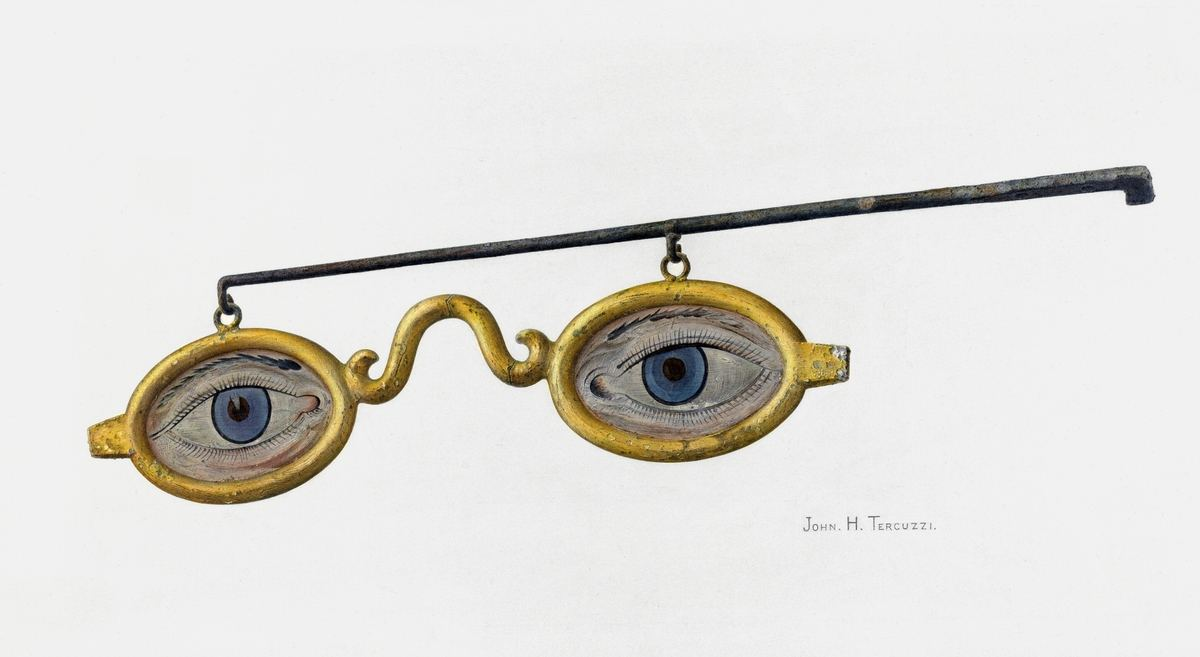
\includegraphics[width=1\linewidth]{imagenes/visualizacion}

La visualización de información es una de las técnica más poderosas, y a la vez más accesibles, de las que disponemos como analistas de datos. La visualización es el proceso de hacer visibles los contrastes, ritmos y eventos que los datos expresan, que no podemos percibir cuando vienen en forma de áridas listas de números y categorías.

Vamos a aprender a realizar las visualizaciones más usadas, y las opciones de ajuste con las que podemos lograr que luzcan tal como queremos.

\hypertarget{una-buena-visualizaciuxf3n-para-empezar-el-scatterplot}{%
\section{\texorpdfstring{Una buena visualización para empezar: el \emph{scatterplot}}{Una buena visualización para empezar: el scatterplot}}\label{una-buena-visualizaciuxf3n-para-empezar-el-scatterplot}}

Los gráficos de dispersión, o \emph{scatterplots}, son quizás el tipo de visualización más conocido. Consisten en puntos proyectados en un eje de coordenadas, donde cada punto representa una observación. Son útiles para mostrar la correlación entre dos variables numéricas.

Por ejemplo, podríamos asumir que existirá una correlación positiva entre la cantidad de habitantes de una comuna y la cantidad anual de delitos. Es decir que, cuantas más personas vivan en una comuna, es de esperarse que sea mayor la cantidad de robos, hurtos, siniestros viales y homicidios que ocurren allí.

Activamos el paquete \texttt{tidyverse}, si aún no lo habíamos hecho.

\begin{Shaded}
\begin{Highlighting}[]
\FunctionTok{library}\NormalTok{(tidyverse)}
\end{Highlighting}
\end{Shaded}

Y si no lo tenemos ya cargado, leemos de nuevo el dataset con los registros de delitos (esta versión incluye la columna ``comuna'').

\begin{Shaded}
\begin{Highlighting}[]
\NormalTok{delitos }\OtherTok{\textless{}{-}} \FunctionTok{read.csv}\NormalTok{(}\StringTok{"https://cdaj.netlify.app/data/delitos\_barrios\_comunas.csv"}\NormalTok{)}
\end{Highlighting}
\end{Shaded}

Usando los verbos de transformación que aprendimos, es fácil obtener un dataframe resumen con indicadores a nivel comuna. Vamos a analizar la cantidad de homicidios.

\begin{Shaded}
\begin{Highlighting}[]
\NormalTok{homicidios\_por\_comuna }\OtherTok{\textless{}{-}}\NormalTok{ delitos }\SpecialCharTok{\%\textgreater{}\%} 
    \FunctionTok{filter}\NormalTok{(tipo }\SpecialCharTok{==} \StringTok{"Homicidio"}\NormalTok{) }\SpecialCharTok{\%\textgreater{}\%} 
    \FunctionTok{group\_by}\NormalTok{(comuna) }\SpecialCharTok{\%\textgreater{}\%} 
    \FunctionTok{summarise}\NormalTok{(}\AttributeTok{homicidios =} \FunctionTok{sum}\NormalTok{(total))}

\NormalTok{homicidios\_por\_comuna}
\end{Highlighting}
\end{Shaded}

\begin{verbatim}
## # A tibble: 15 x 2
##    comuna homicidios
##     <int>      <int>
##  1      1         44
##  2      2          6
##  3      3         17
##  4      4         31
##  5      5          5
##  6      6          5
##  7      7         17
##  8      8         18
##  9      9          9
## 10     10          4
## 11     11          8
## 12     12          7
## 13     13         10
## 14     14          8
## 15     15         12
\end{verbatim}

Lo que nos falta ahora es la cantidad de habitantes en cada comuna. \emph{No problem}. El dato es fácil de conseguir, otra vez cortesía de la Dirección General de Estadística y Censos de la Ciudad de Buenos Aires. Traemos la proyección al año 2020 de la cantidad de habitantes por comuna.

\begin{Shaded}
\begin{Highlighting}[]
\NormalTok{poblacion }\OtherTok{\textless{}{-}} \FunctionTok{read.csv}\NormalTok{(}\StringTok{"https://cdaj.netlify.app/data/comunas\_poblacion\_2020.csv"}\NormalTok{)}

\NormalTok{poblacion}
\end{Highlighting}
\end{Shaded}

\begin{verbatim}
##    comuna poblacion
## 1       1    256405
## 2       2    149430
## 3       3    193276
## 4       4    240100
## 5       5    187518
## 6       6    185456
## 7       7    241861
## 8       8    228953
## 9       9    171264
## 10     10    170592
## 11     11    190076
## 12     12    214777
## 13     13    236358
## 14     14    227115
## 15     15    182465
\end{verbatim}

Por suerte, ya sabemos como combinar tablas usando \texttt{left\_join()}

\begin{Shaded}
\begin{Highlighting}[]
\NormalTok{homicidios\_por\_comuna }\OtherTok{\textless{}{-}}\NormalTok{ homicidios\_por\_comuna }\SpecialCharTok{\%\textgreater{}\%} \FunctionTok{left\_join}\NormalTok{(poblacion)}

\NormalTok{homicidios\_por\_comuna}
\end{Highlighting}
\end{Shaded}

\begin{verbatim}
## # A tibble: 15 x 3
##    comuna homicidios poblacion
##     <int>      <int>     <int>
##  1      1         44    256405
##  2      2          6    149430
##  3      3         17    193276
##  4      4         31    240100
##  5      5          5    187518
##  6      6          5    185456
##  7      7         17    241861
##  8      8         18    228953
##  9      9          9    171264
## 10     10          4    170592
## 11     11          8    190076
## 12     12          7    214777
## 13     13         10    236358
## 14     14          8    227115
## 15     15         12    182465
\end{verbatim}

!Preparativos terminados! Hagamos por fin nuestro \emph{scatterplot}. Tal como en el capítulo de introducción a R, continuaremos usando \texttt{ggplot()} para visualizar:

\begin{Shaded}
\begin{Highlighting}[]
\FunctionTok{ggplot}\NormalTok{(homicidios\_por\_comuna)}
\end{Highlighting}
\end{Shaded}

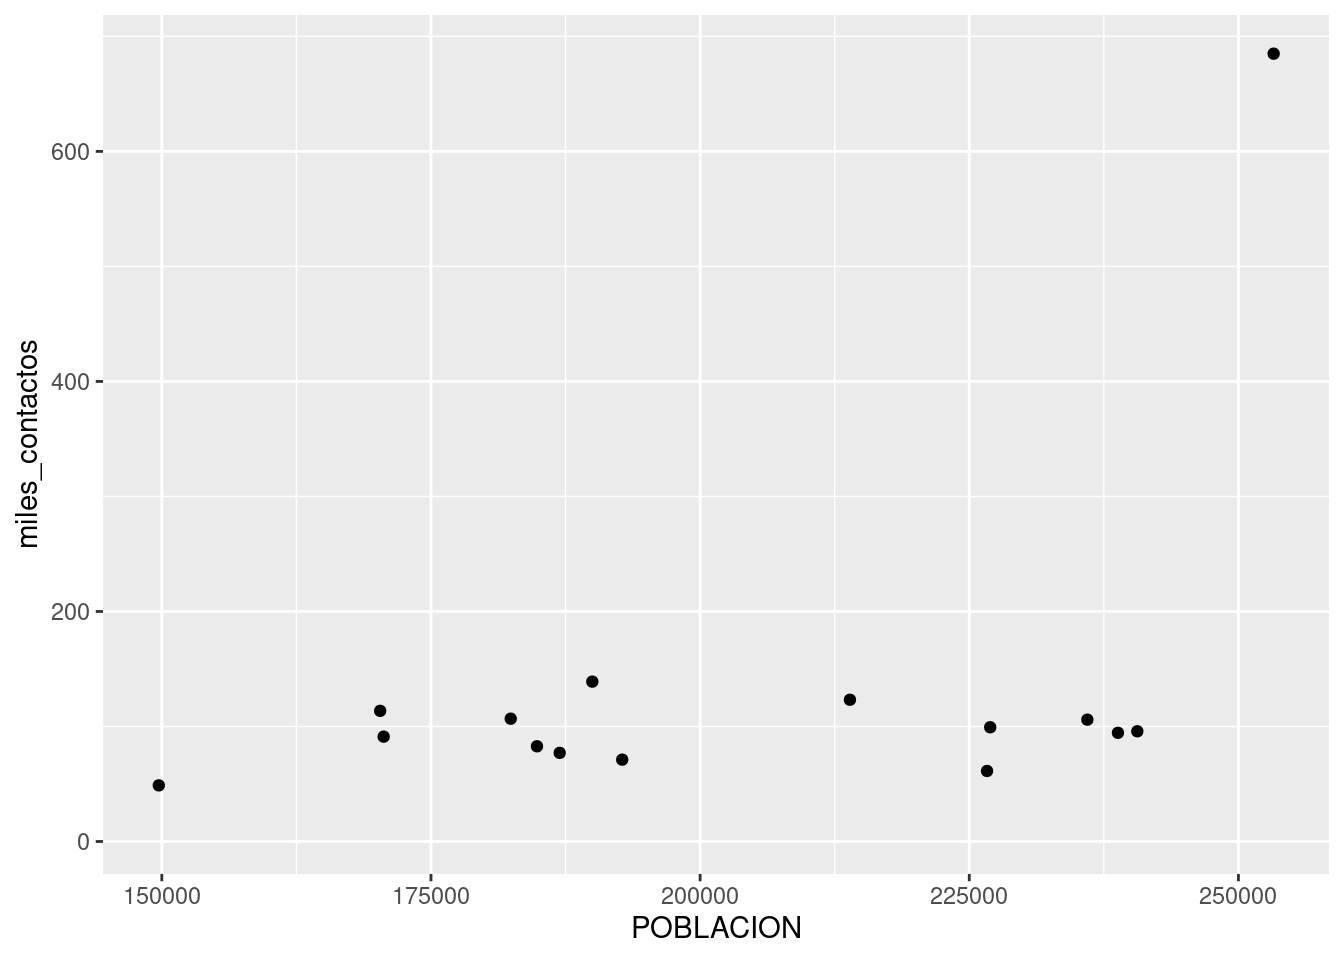
\includegraphics{CD_AJ_files/figure-latex/unnamed-chunk-89-1.pdf}

¿Un gráfico vacío? Recordemos que ggplot funciona por capas. Primero uno declara el dataframe que va a usar, y luego agrega una o más capas con representaciones de la información. La forma de agregar una capa con un scatterplot, en la práctica dibujar puntos, es con \texttt{geom\_point}:

\begin{Shaded}
\begin{Highlighting}[]
\FunctionTok{ggplot}\NormalTok{(homicidios\_por\_comuna) }\SpecialCharTok{+} \FunctionTok{geom\_point}\NormalTok{(}\FunctionTok{aes}\NormalTok{(}\AttributeTok{x =}\NormalTok{ poblacion, }\AttributeTok{y =}\NormalTok{ homicidios))}
\end{Highlighting}
\end{Shaded}

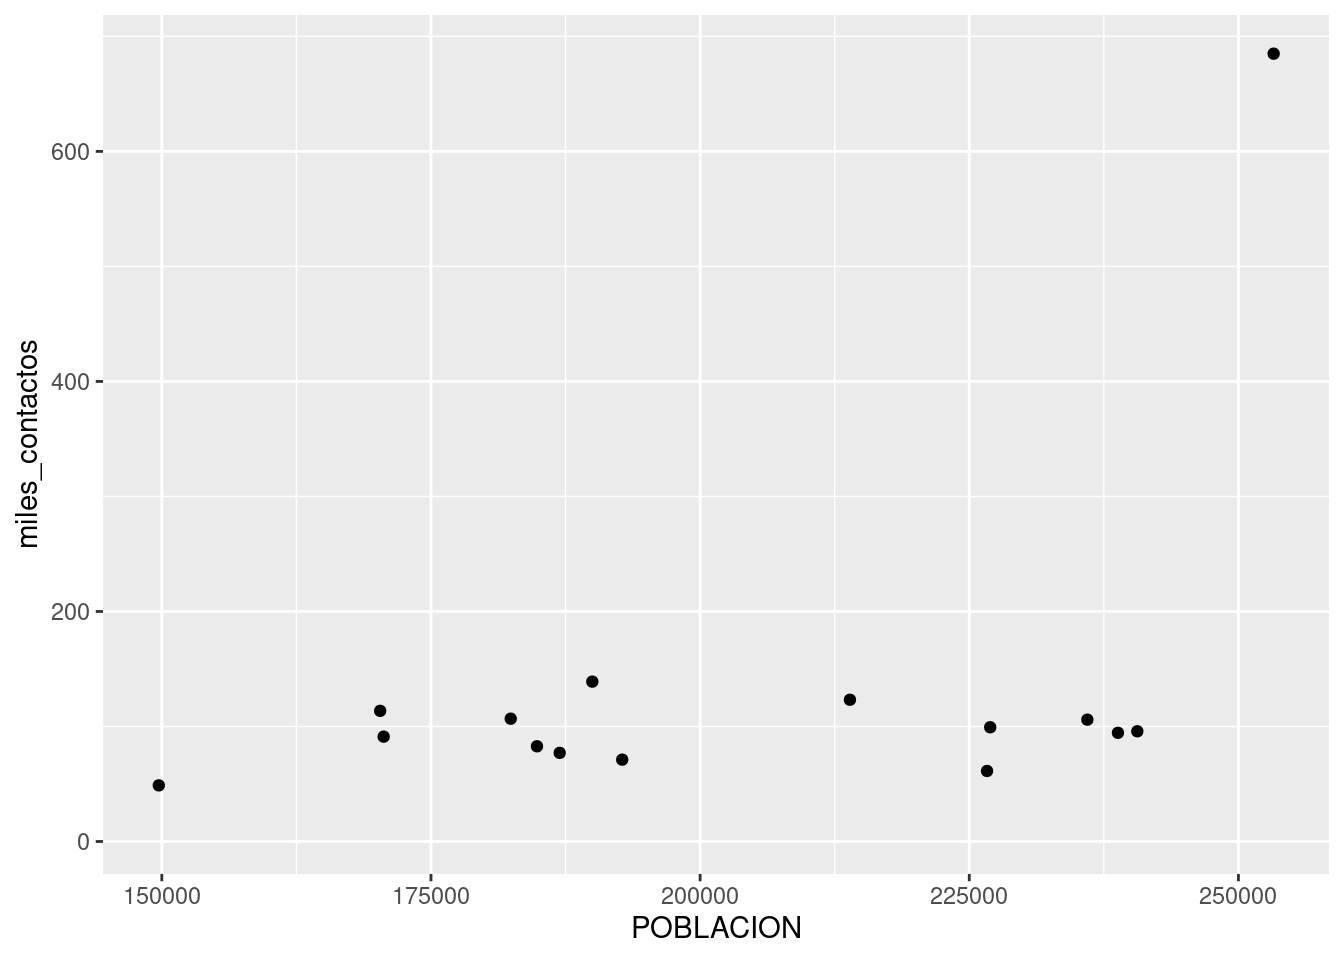
\includegraphics{CD_AJ_files/figure-latex/unnamed-chunk-90-1.pdf}

Lo que hicimos fue pedirle a ggplot que dibuje un punto por cada fila (representando a cada comuna), con la posición en el eje de las \texttt{x} según su población, y en el eje de las \texttt{y} según la cantidad de contactos registrados. Estas referencias estéticas (\emph{aesthetics} en inglés) son las que van dentro de la función \texttt{aes()} en \texttt{geom\_point(aes(x\ =\ poblacion,\ y\ =\ homicidios))}

En el extremo superior derecho hay una comuna que sobresale. Podemos identificarla, pidiendo a ggplot que agregue una variable más a la visualización -la comuna. Siendo un gráfico en dos dimensiones, ya no podemos usar la posición para representar un valor; tanto la posición horizontal como la vertical están siendo usadas por población y total. Nuestras opciones son codificar la comuna por color, forma o tamaño del punto. A pesar de que son identificadas con números, las comunas son una variable categórica: no tiene sentido decir que la comuna 1 es ``menor'' que la comuna 7. Par las variables categóricas, el color suele ser una buena opción de codificación.

Lo hacemos agregando un parámetro \texttt{color} dentro de \texttt{aes()}. Tal como hicimos en el capítulo 2, usamos \texttt{factor(comuna)} en lugar de \texttt{comuna} a secas para indicarle a R que queremos que trate a la variable como categórica:

\begin{Shaded}
\begin{Highlighting}[]
\FunctionTok{ggplot}\NormalTok{(homicidios\_por\_comuna) }\SpecialCharTok{+} 
    \FunctionTok{geom\_point}\NormalTok{(}\FunctionTok{aes}\NormalTok{(}\AttributeTok{x =}\NormalTok{ poblacion, }\AttributeTok{y =}\NormalTok{ homicidios, }\AttributeTok{color =} \FunctionTok{factor}\NormalTok{(comuna)))}
\end{Highlighting}
\end{Shaded}

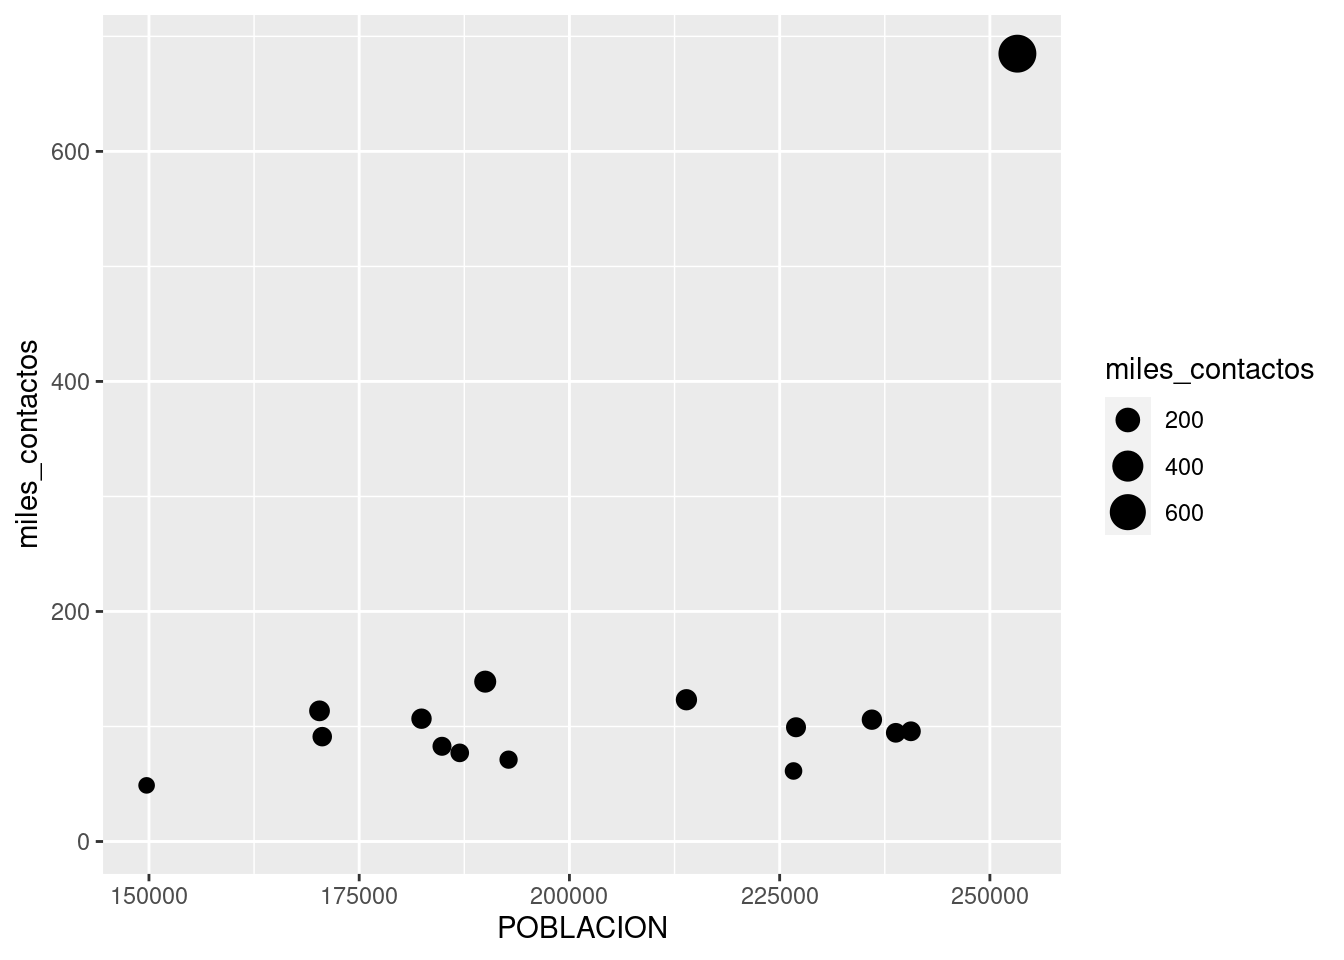
\includegraphics{CD_AJ_files/figure-latex/unnamed-chunk-91-1.pdf}

En ese caso, no es tan fácil discernir cuál es cuál, pero mirando con cuidado descubrimos que la comuna 1 es la que tiene mayor población y donde se reportaó la mayor cantidad de homicidios. Lo que nos pasa aquí es que tenemos demasiadas categorías, con lo cual cada una tiene su propio color pero el rango cromático no alcanza para darle a cada una un tono bien distinto al de las demás.

Si necesitamos generar un gráfico que no deje lugar a dudas, lo resolvemos usando un método alternativo para el scatterplot. En lugar de dibujar puntos, podemos poner etiquetas con el nombre de cada comuna.

En lugar de

\begin{Shaded}
\begin{Highlighting}[]
\FunctionTok{ggplot}\NormalTok{(homicidios\_por\_comuna) }\SpecialCharTok{+} 
    \FunctionTok{geom\_point}\NormalTok{(}\FunctionTok{aes}\NormalTok{(}\AttributeTok{x =}\NormalTok{ poblacion, }\AttributeTok{y =}\NormalTok{ homicidios, }\AttributeTok{color =} \FunctionTok{factor}\NormalTok{(comuna)))}
\end{Highlighting}
\end{Shaded}

usamos

\begin{Shaded}
\begin{Highlighting}[]
\FunctionTok{ggplot}\NormalTok{(homicidios\_por\_comuna) }\SpecialCharTok{+} 
    \FunctionTok{geom\_label}\NormalTok{(}\FunctionTok{aes}\NormalTok{(}\AttributeTok{x =}\NormalTok{ poblacion, }\AttributeTok{y =}\NormalTok{ homicidios, }\AttributeTok{label =} \FunctionTok{factor}\NormalTok{(comuna)))}
\end{Highlighting}
\end{Shaded}

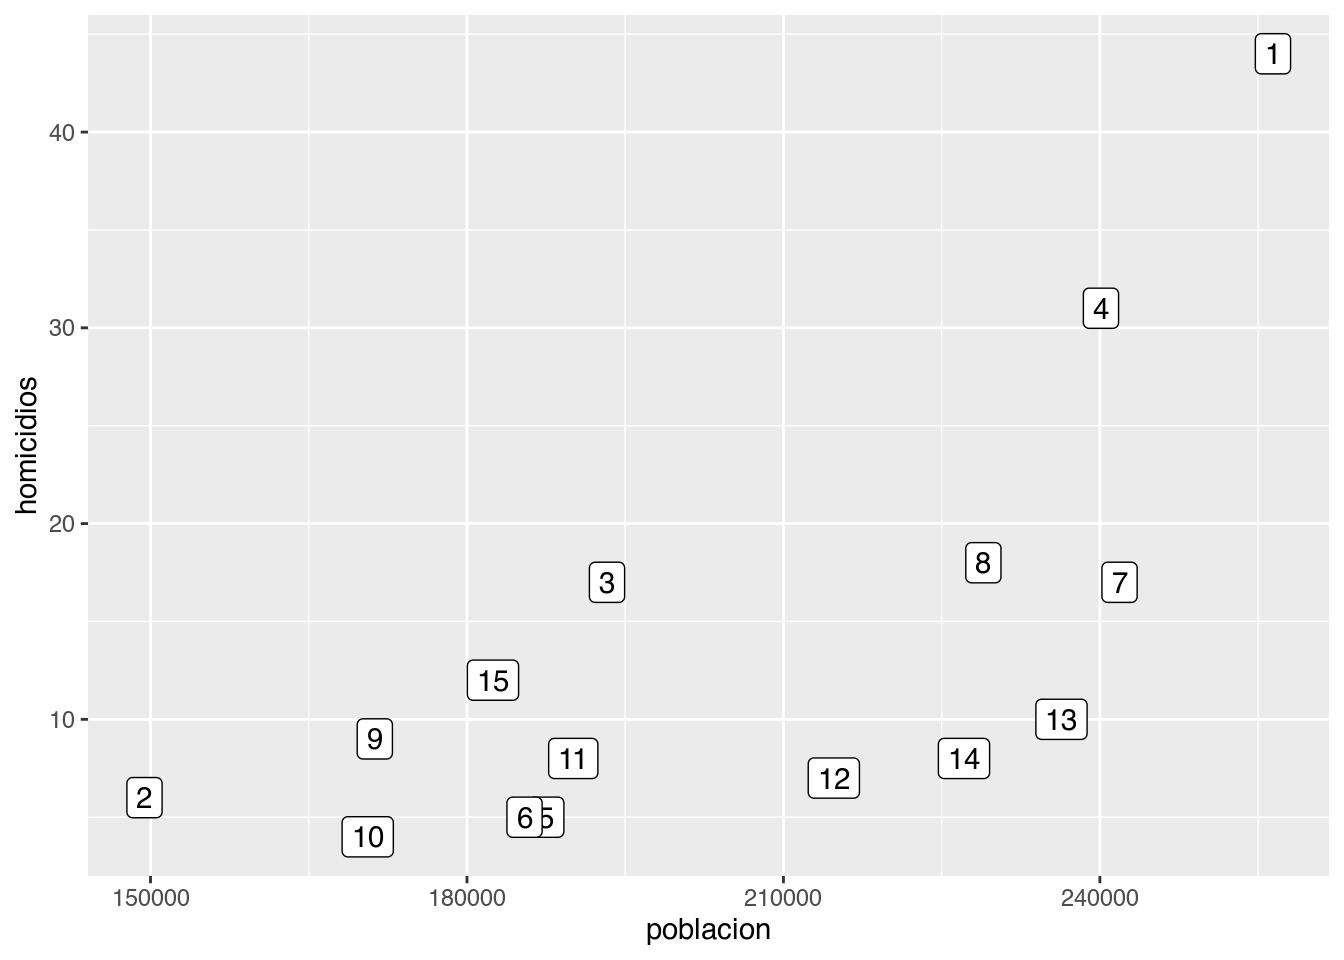
\includegraphics{CD_AJ_files/figure-latex/unnamed-chunk-93-1.pdf}

Volvamos a nuestros puntos para practicar dos codificaciones estéticas que no hemos probado, color y tamaño.

Para dejar aún más clara la diferencia de homicidios entre comunas, podríamos usar el tamaño (\emph{size}) de cada punto para representar esa variable, además de su altura en el gráfico.

\begin{Shaded}
\begin{Highlighting}[]
\FunctionTok{ggplot}\NormalTok{(homicidios\_por\_comuna) }\SpecialCharTok{+} 
    \FunctionTok{geom\_point}\NormalTok{(}\FunctionTok{aes}\NormalTok{(}\AttributeTok{x =}\NormalTok{ poblacion, }\AttributeTok{y =}\NormalTok{ homicidios, }\AttributeTok{size =}\NormalTok{ homicidios))}
\end{Highlighting}
\end{Shaded}

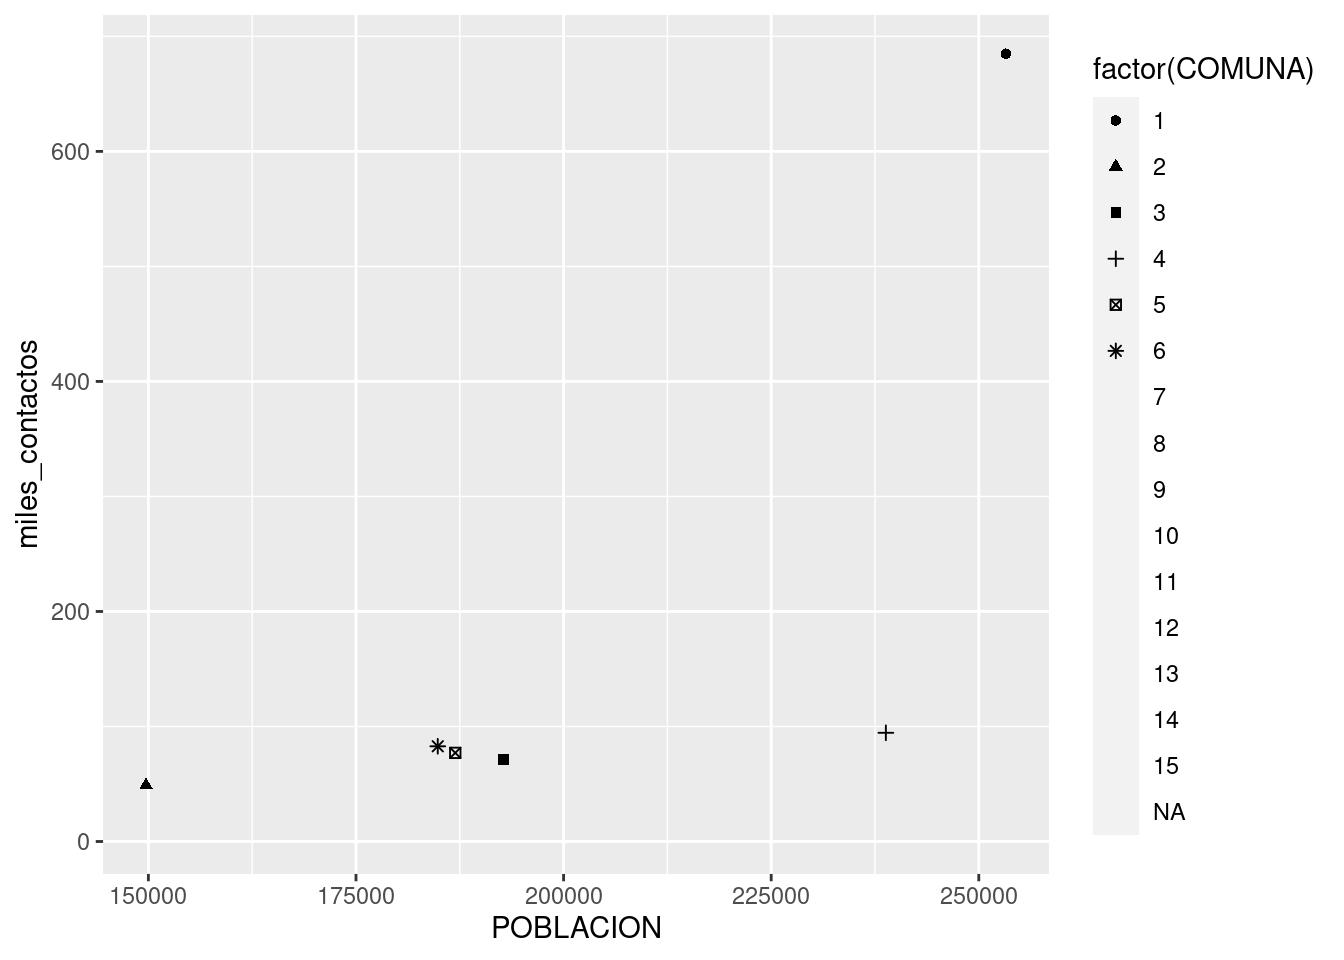
\includegraphics{CD_AJ_files/figure-latex/unnamed-chunk-94-1.pdf}

Y para distinguir cuál es cuál, podemos pedirle a ggplot que cambie la forma (\emph{shape}) de cada punto según la comuna a la que corresponde.

\begin{Shaded}
\begin{Highlighting}[]
\FunctionTok{ggplot}\NormalTok{(homicidios\_por\_comuna) }\SpecialCharTok{+} 
    \FunctionTok{geom\_point}\NormalTok{(}\FunctionTok{aes}\NormalTok{(}\AttributeTok{x =}\NormalTok{ poblacion, }\AttributeTok{y =}\NormalTok{ homicidios, }\AttributeTok{shape =} \FunctionTok{factor}\NormalTok{(comuna)))}
\end{Highlighting}
\end{Shaded}

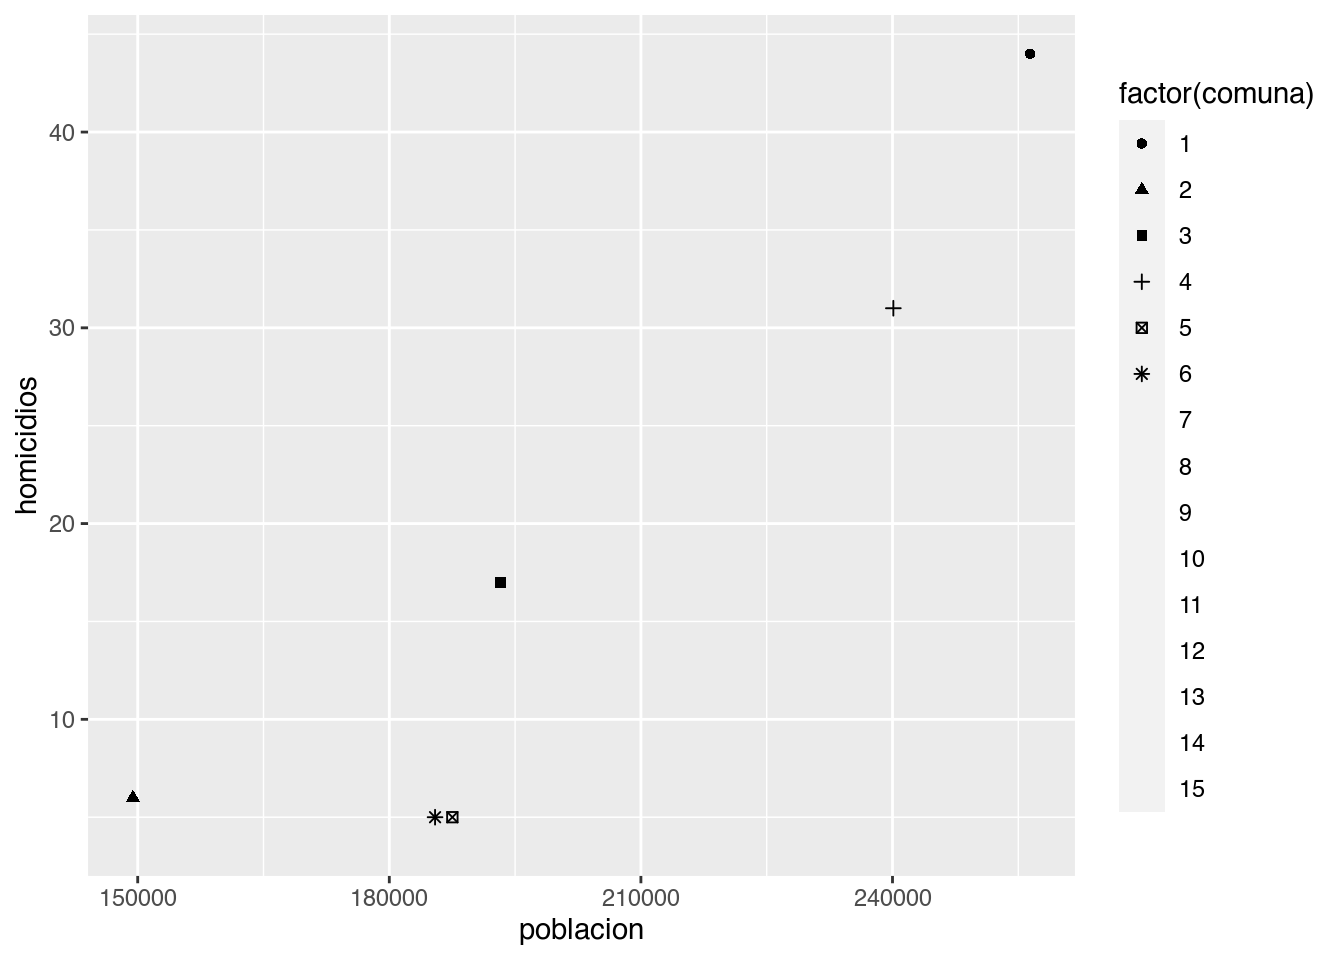
\includegraphics{CD_AJ_files/figure-latex/unnamed-chunk-95-1.pdf}

¡Hey, sólo aparecen seis de las comunas! \texttt{ggplot()} usa cómo máximo 6 formas distintas, debido a que una cantidad mayor sería de veras muy difícil de discernir para nuestros pobres ojos. Moraleja: la estética \texttt{shape} sirve sólo cuando manejamos pocas categorías. De todas formas podría opinarse que es el método de codificación que menos gracia tiene, así que no es grave que su utilidad sea limitada.

\hypertarget{ajustando-color-y-tamauxf1o}{%
\section{Ajustando color y tamaño}\label{ajustando-color-y-tamauxf1o}}

Hemos visto que especificando atributos estéticos y las variables que representan dentro
de \texttt{aes()} podemos ajustas posición, tamaño, color y hasta la forma de los puntos de acuerdo a sus valores. Pero, ¿qué pasa si queremos usar un tamaño o un color arbitrario para nuestros puntos? Es decir, si no nos gusta el color negro y queremos que sean todos azules, o si nos parece que se ven pequeños y queremos que sean todos un poco más grandes. Fácil: definimos el \texttt{color} o \texttt{size} que queremos por fuera de las función \texttt{aes()}, y será aplicado a todos los puntos.

\begin{Shaded}
\begin{Highlighting}[]
\FunctionTok{ggplot}\NormalTok{(homicidios\_por\_comuna) }\SpecialCharTok{+} 
    \FunctionTok{geom\_point}\NormalTok{(}\FunctionTok{aes}\NormalTok{(}\AttributeTok{x =}\NormalTok{ poblacion, }\AttributeTok{y =}\NormalTok{ homicidios), }\AttributeTok{color =} \StringTok{"blue"}\NormalTok{)}
\end{Highlighting}
\end{Shaded}

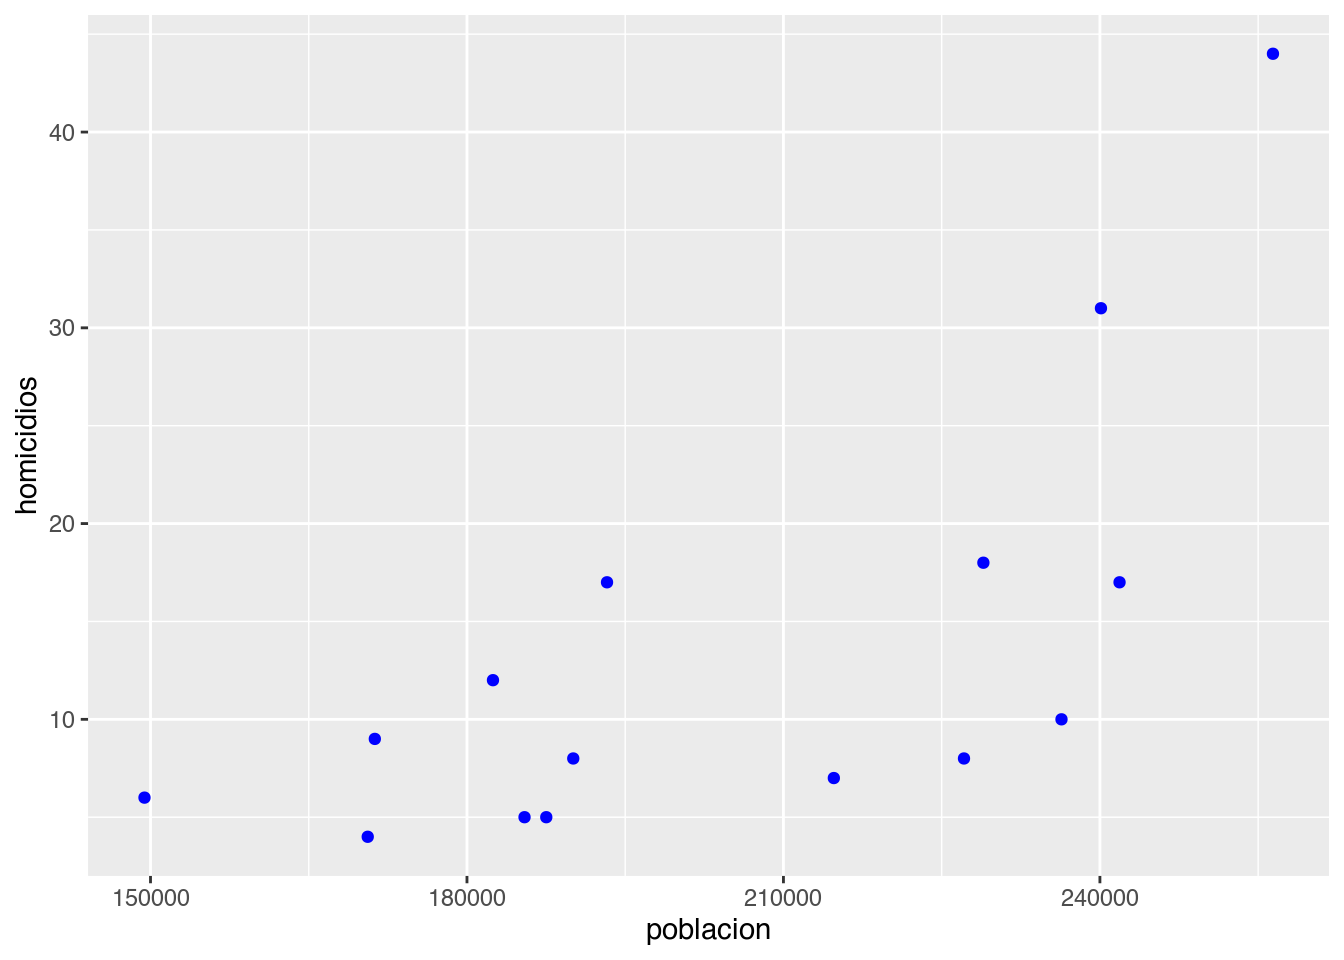
\includegraphics{CD_AJ_files/figure-latex/unnamed-chunk-96-1.pdf}

Obsérvese que \texttt{color\ =\ "blue"} está escrito por fuera de los paréntesis de \texttt{aes()}. De paso, hicimos uso de una característica muy práctica de R: reconoce un montón de colores por su nombre, siempre que los escribamos entre comillas. Si le decimos \texttt{color\ =\ "blue"}, \texttt{color\ =\ "red"}, \texttt{color\ =\ "yellow"}, etc., sabe de que hablamos. Una lista de todos los colores que R reconoce, ideal como referencia, se puede encontrar en \url{http://www.stat.columbia.edu/~tzheng/files/Rcolor.pdf} ; ¡son más de 600!.

Tras un vistazo a la lista, me decido por ``darkolivegreen4'':

\begin{Shaded}
\begin{Highlighting}[]
\FunctionTok{ggplot}\NormalTok{(homicidios\_por\_comuna) }\SpecialCharTok{+} 
    \FunctionTok{geom\_point}\NormalTok{(}\FunctionTok{aes}\NormalTok{(}\AttributeTok{x =}\NormalTok{ poblacion, }\AttributeTok{y =}\NormalTok{ homicidios), }\AttributeTok{color =} \StringTok{"darkolivegreen4"}\NormalTok{)}
\end{Highlighting}
\end{Shaded}

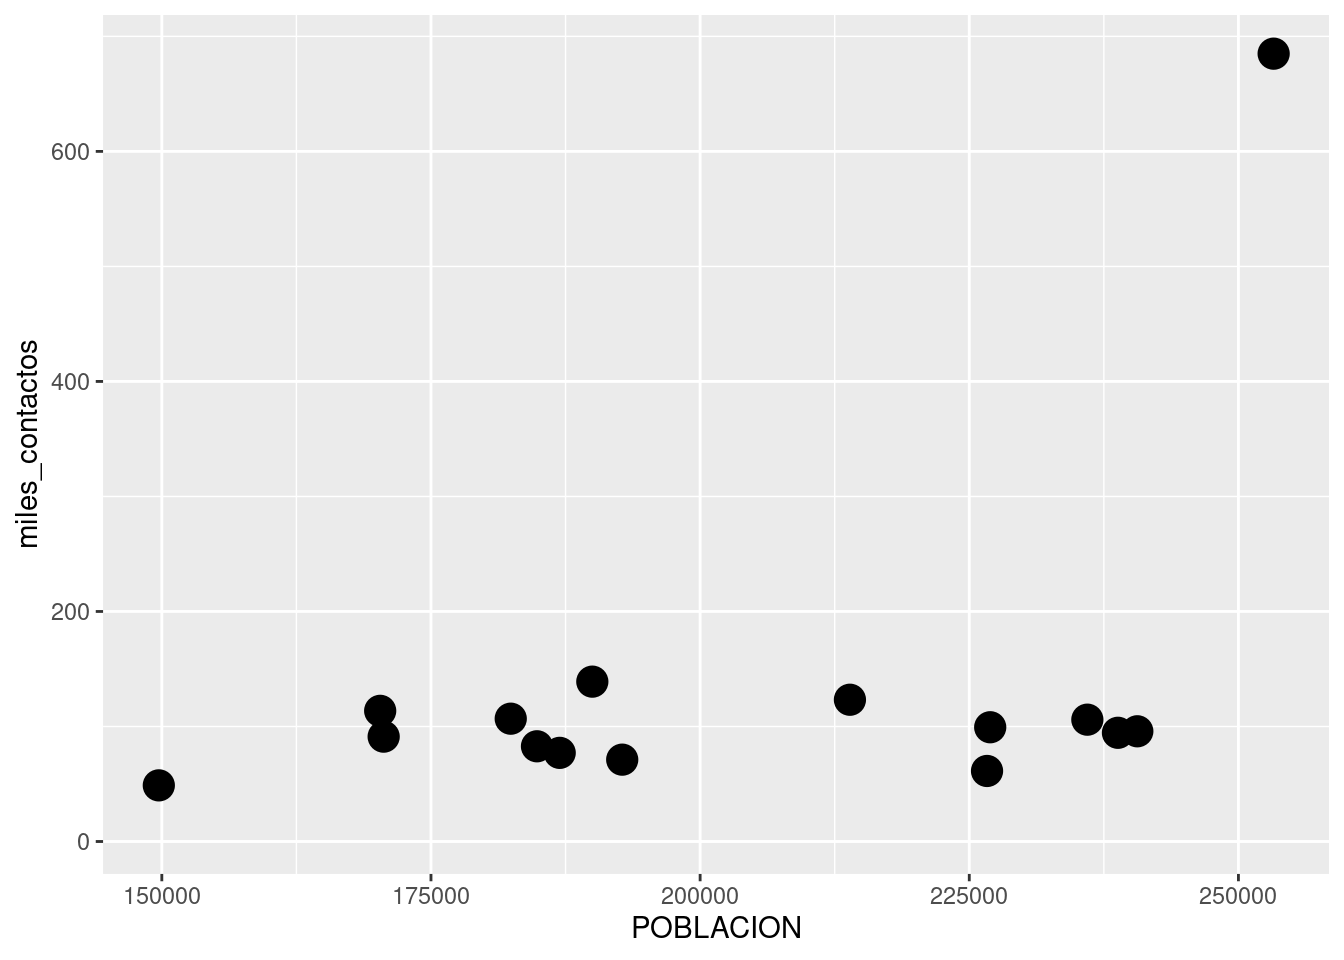
\includegraphics{CD_AJ_files/figure-latex/unnamed-chunk-97-1.pdf}

Queda claro que podemos asignar el color que queramos.

En cuanto al tamaño, la fórmula es la misma:

\begin{Shaded}
\begin{Highlighting}[]
\FunctionTok{ggplot}\NormalTok{(homicidios\_por\_comuna) }\SpecialCharTok{+} 
    \FunctionTok{geom\_point}\NormalTok{(}\FunctionTok{aes}\NormalTok{(}\AttributeTok{x =}\NormalTok{ poblacion, }\AttributeTok{y =}\NormalTok{ homicidios), }\AttributeTok{size =} \DecValTok{5}\NormalTok{)}
\end{Highlighting}
\end{Shaded}

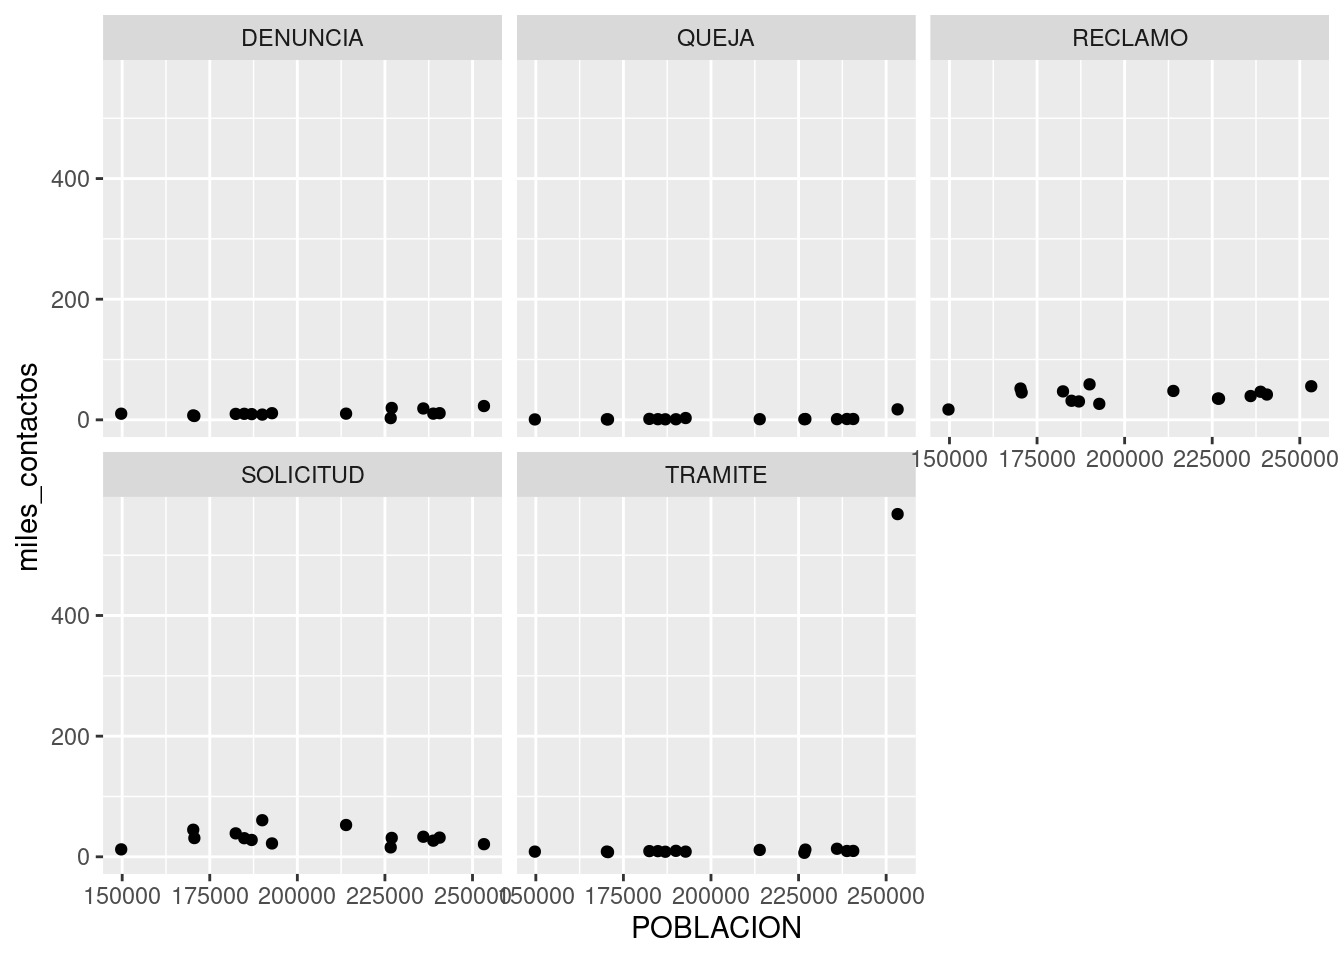
\includegraphics{CD_AJ_files/figure-latex/unnamed-chunk-98-1.pdf}

El valor de \texttt{size} se da en píxeles. Es una medida difícil de estimar antes de ver el resultado, pero es cuestión de probar algunos valores distintos hasta encontrar el que nos va bien. Por supuesto, podemos ajustar varios, o todos, los atributos a la vez

\begin{Shaded}
\begin{Highlighting}[]
\FunctionTok{ggplot}\NormalTok{(homicidios\_por\_comuna) }\SpecialCharTok{+} 
    \FunctionTok{geom\_point}\NormalTok{(}\FunctionTok{aes}\NormalTok{(}\AttributeTok{x =}\NormalTok{ poblacion, }\AttributeTok{y =}\NormalTok{ homicidios), }
               \AttributeTok{size =} \DecValTok{9}\NormalTok{, }\AttributeTok{color =} \StringTok{"chocolate3"}\NormalTok{, }\AttributeTok{shape =} \DecValTok{0}\NormalTok{)}
\end{Highlighting}
\end{Shaded}

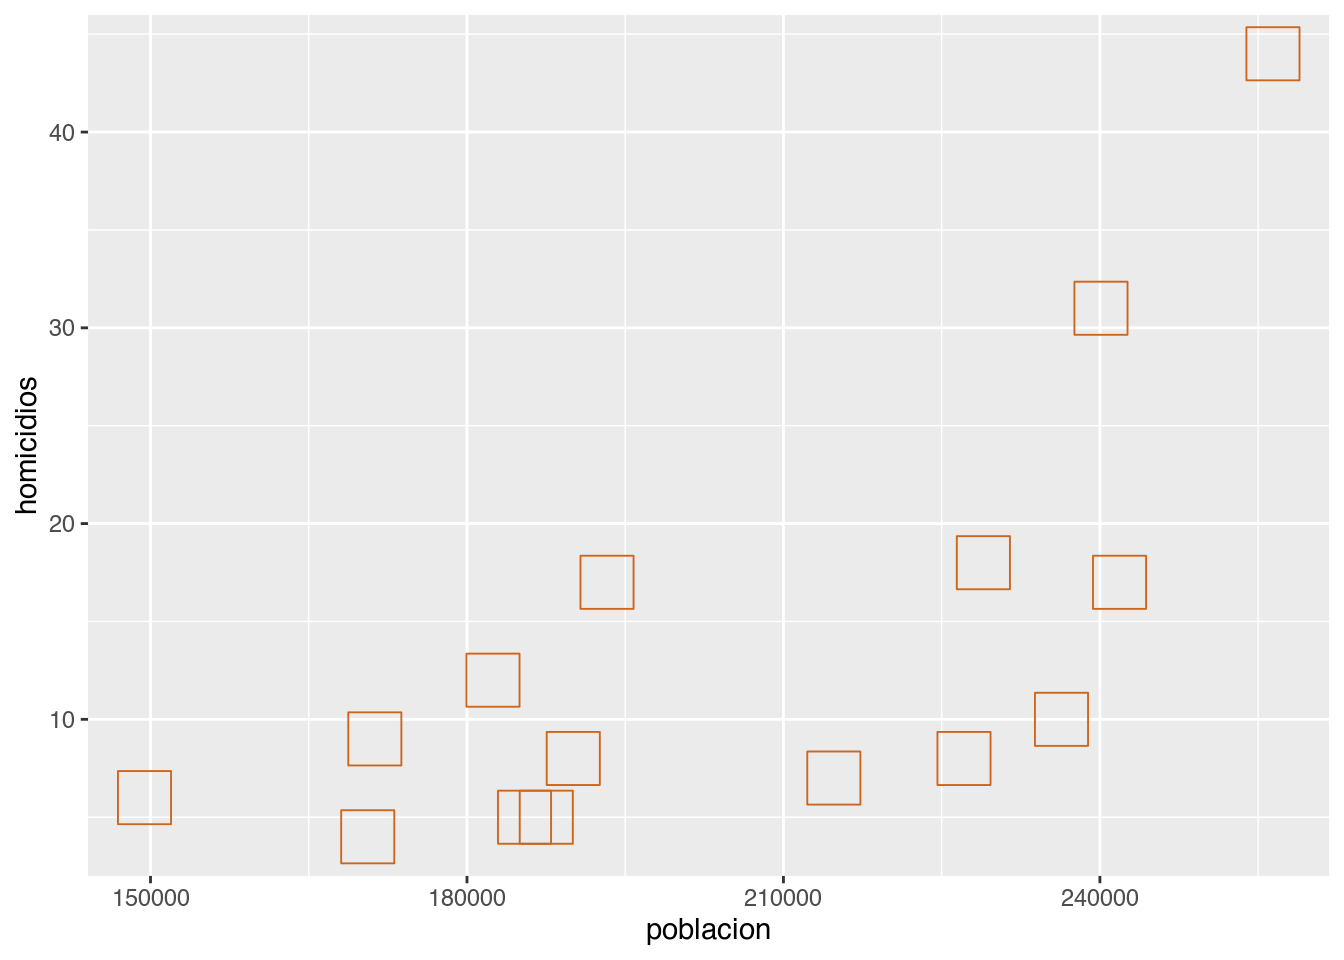
\includegraphics{CD_AJ_files/figure-latex/unnamed-chunk-99-1.pdf}

\hypertarget{facetado}{%
\section{Facetado}\label{facetado}}

Ya sabemos como representar variables usando atributos estéticos. Con esa técnica podemos mostrar con claridad dos o tres variables en un plano bidimensional (nuestro gráfico). Pero cuando si queremos agregar más atributos para codificar variables adicionales, la visualización pierde legibilidad de inmediato. Por suerte existe otra técnica, que podemos usar en combinación con la estética, para agregar aún más variables: el facetado.

Las facetas son múltiples gráficos contiguos, con cada uno mostrando un subconjunto de los datos. Son útiles sobre todo para variables categóricas.

Practiquemos con un ejemplo. Sabemos que en la comuna 1 se registra una cantidad de homicidios mayor que en las demás. ¿La diferencia será igual para todas las categorías de homicidio, o existe alguna en particular que es la que inclina la balanza?

En nuestro dataframe original, para cada incidente tenemos las columnas ``tipo'' y ``subtipo''. Para revisar rápido cuales son las combinaciones posibles de éstas categorías podemos armar una \emph{tabla de contingencia}, un conteo de las combinaciones de categorías según aparecen en nuestros datos. Presentemos entonces a la función \texttt{count()}, que nos puede dar una mano.

\begin{Shaded}
\begin{Highlighting}[]
\NormalTok{delitos }\SpecialCharTok{\%\textgreater{}\%} 
    \FunctionTok{count}\NormalTok{(tipo, subtipo)}
\end{Highlighting}
\end{Shaded}

\begin{verbatim}
##                     tipo                      subtipo   n
## 1              Homicidio                       Doloso  81
## 2              Homicidio                    Femicidio  10
## 3              Homicidio      Femicidio Intrafamiliar   1
## 4              Homicidio               Siniestro Vial  69
## 5              Homicidio Travesticidio/Transfemicidio   2
## 6  Hurto (sin violencia)                              583
## 7  Hurto (sin violencia)              Hurto Automotor 504
## 8               Lesiones               Siniestro Vial 575
## 9   Robo (con violencia)                              583
## 10  Robo (con violencia)              Con uso de moto 517
## 11  Robo (con violencia)               Robo Automotor 263
\end{verbatim}

Para el tipo ``Homicidio'' encontramos los subtipos ``Doloso'', ``Femicidio'', ``Femicidio Intrafamiliar'', ``Siniestro Vial'', y ``Travesticidio/Transfemicidio''. Podemos usar esas subcategorías para mostrar como componen el total de homicidios de cada comuna.

Agrupamos entonces nuestra data de homicidios por comuna y también por subtipo, sin olvidar agregar luego los datos de población

\begin{Shaded}
\begin{Highlighting}[]
\NormalTok{homicidios\_por\_comuna\_y\_subtipo }\OtherTok{\textless{}{-}}\NormalTok{ delitos }\SpecialCharTok{\%\textgreater{}\%} 
    \FunctionTok{filter}\NormalTok{(tipo }\SpecialCharTok{==} \StringTok{"Homicidio"}\NormalTok{) }\SpecialCharTok{\%\textgreater{}\%} 
    \FunctionTok{group\_by}\NormalTok{(comuna, subtipo) }\SpecialCharTok{\%\textgreater{}\%} 
    \FunctionTok{summarise}\NormalTok{(}\AttributeTok{homicidios =} \FunctionTok{sum}\NormalTok{(total)) }\SpecialCharTok{\%\textgreater{}\%} 
    \FunctionTok{left\_join}\NormalTok{(poblacion)}

\FunctionTok{head}\NormalTok{(homicidios\_por\_comuna\_y\_subtipo)}
\end{Highlighting}
\end{Shaded}

\begin{verbatim}
## # A tibble: 6 x 4
## # Groups:   comuna [3]
##   comuna subtipo        homicidios poblacion
##    <int> <chr>               <int>     <int>
## 1      1 Doloso                 32    256405
## 2      1 Femicidio               1    256405
## 3      1 Siniestro Vial         11    256405
## 4      2 Doloso                  2    149430
## 5      2 Siniestro Vial          4    149430
## 6      3 Doloso                  6    193276
\end{verbatim}

Listos para facetar. Producimos un scatterplot igual que antes, y le agregamos una capa adicional con \texttt{facet\_wrap()}. La variable a ``facetar'', la que recibirá un gráfico por cada una de sus categorías, siempre se escribe a continuación del signo \texttt{\textasciitilde{}}; en nuestro caso, queda como \texttt{\textasciitilde{}subtipo}. El simbolillo en cuestión denota lo que en R se denomina una \emph{fórmula} y ya nos lo cruzaremos de nuevo, pero por ahora no le prestamos más atención.

\begin{Shaded}
\begin{Highlighting}[]
\FunctionTok{ggplot}\NormalTok{(homicidios\_por\_comuna\_y\_subtipo) }\SpecialCharTok{+} 
    \FunctionTok{geom\_point}\NormalTok{(}\FunctionTok{aes}\NormalTok{(}\AttributeTok{x =}\NormalTok{ poblacion, }\AttributeTok{y =}\NormalTok{ homicidios)) }\SpecialCharTok{+}
    \FunctionTok{facet\_wrap}\NormalTok{(}\SpecialCharTok{\textasciitilde{}}\NormalTok{subtipo)}
\end{Highlighting}
\end{Shaded}

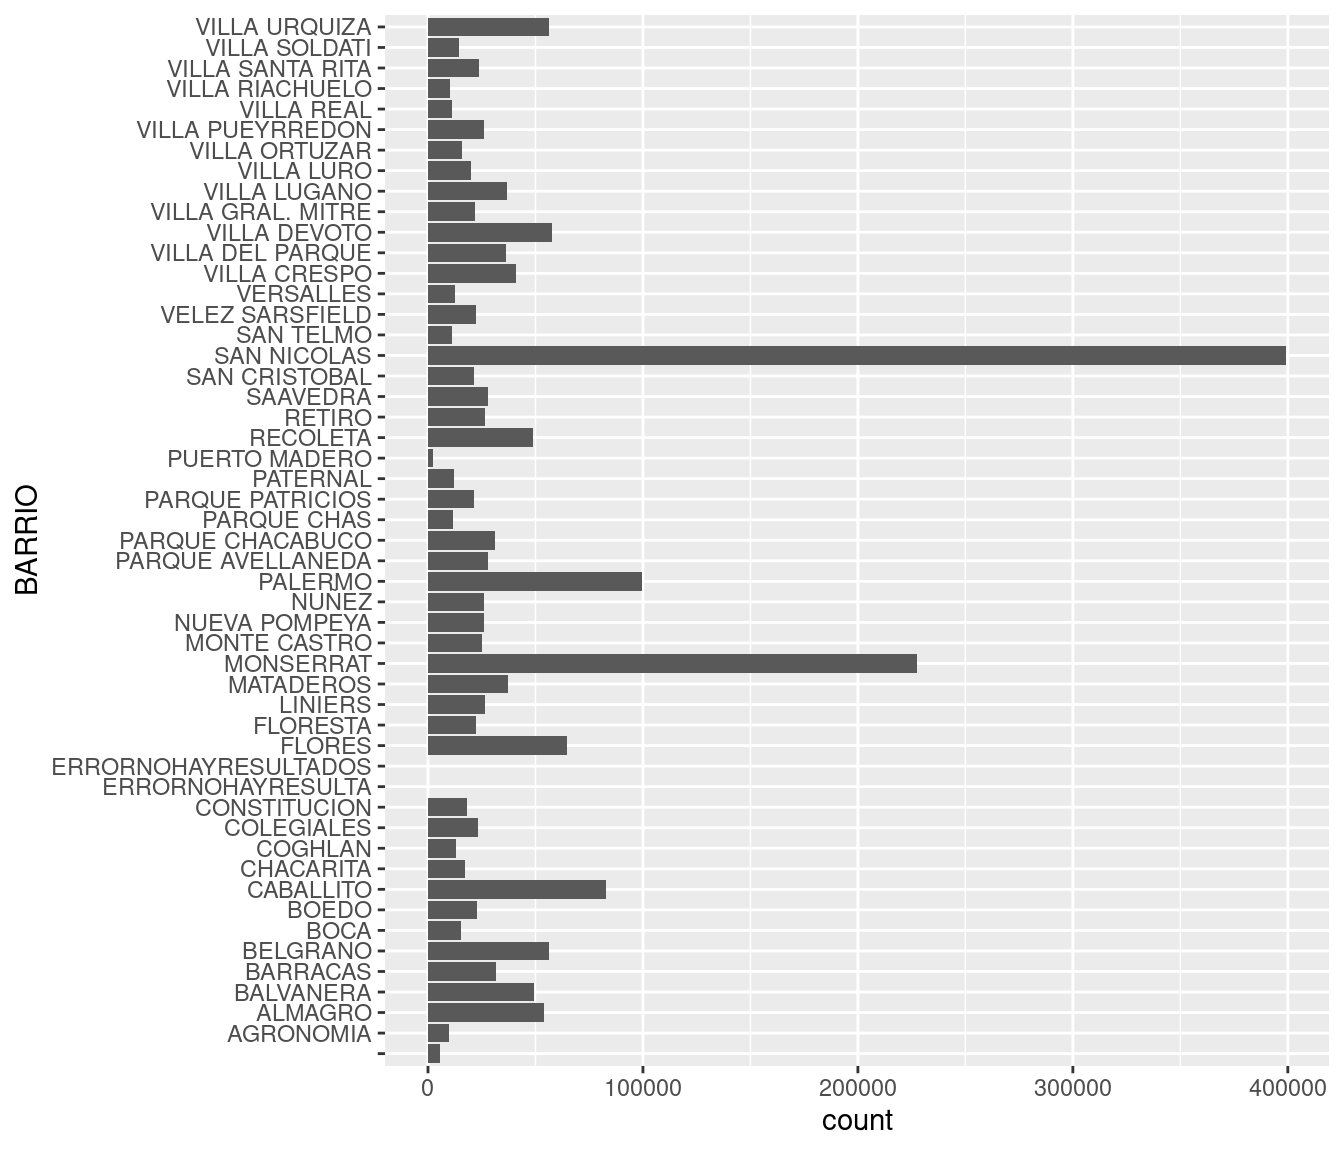
\includegraphics{CD_AJ_files/figure-latex/unnamed-chunk-102-1.pdf}

La notable cantidad de casos en la comuna 1 se debe a los homicidios dolosos; en ninguna otra categoría se separa tanto del resto. ¿Qué tiene de particular esta comuna? Es la más poblada, si, pero aún en proporción per cápita parece separarse de las demás (junto con otra comuna, la 4, que le sigue en población y en número de casos).

Vale la pregunta, por ahora sin respuesta, para mencionar algo fundamental: por más ciencia de datos que apliquemos, siempre vamos a llegar a un punto en que nuestros hallazgos no tendrán sentido sin combinarlos con lo que se llama ``conocimiento de dominio''. El conocimiento de dominio es el saber especializado sobre el tema que estamos tratando, sea el ciclo reproductivo de la gaviota austral o la organización administrativa del Gobierno de la Ciudad Autónoma de Buenos Aires. Esto no debería desanimarnos, ¡al contrario!. El análisis de datos como profesión conlleva un constante aprendizaje sobre los más variados temas. Y a la inversa: si somos expertos en cualquier campo, aún con un puñado de técnicas básicas de R podemos extraer conocimiento de nuestros datos que jamas encontraría una persona, aún experta en programación, que no conozca el contexto.

\hypertarget{gruxe1ficos-de-barras}{%
\section{Gráficos de barras}\label{gruxe1ficos-de-barras}}

Si hay un tipo de visualización que compite en popularidad con el \emph{scatterplot}, son los gráficos de barras (\emph{bar charts} en inglés). Solemos encontrarlos acompañando artículos en diarios y revistas, sin duda porque son fáciles de leer de un vistazo. Los gráficos de barras se usan mucho para hacer comparaciones: quién tiene más y quién tiene menos de alguna variable continua cómo ingresos, edad, altura o similares.

Comparemos la suma total de registros que alcanza cada barrio. Con \texttt{geom\_bar} podemos agregar una capa de visualización con gráficos de barras. Los parámetros a definir dentro de \texttt{aes()} son \texttt{x}, donde va una variable categórica, y en forma opcional \texttt{weight}, que indica la variable a sumar para determinar la altura de cada barra. Si no especificamos un \texttt{weight}, simplemente se cuenta cuantas veces aparece cada categoría en el dataframe, en la práctica un conteo o frecuencia de aparición. En nuestro dataset cada fila incluye un período y un total de contactos recibidos. Nosotros no estamos interesados en cuantas veces aparece cada barrio, sino en la suma de la columna total para cada uno de ellos, así que vamos a usar \texttt{weight\ =\ total}.

\begin{Shaded}
\begin{Highlighting}[]
\FunctionTok{ggplot}\NormalTok{(delitos) }\SpecialCharTok{+}
    \FunctionTok{geom\_bar}\NormalTok{(}\FunctionTok{aes}\NormalTok{(}\AttributeTok{x =}\NormalTok{ barrio, }\AttributeTok{weight =}\NormalTok{ total))}
\end{Highlighting}
\end{Shaded}

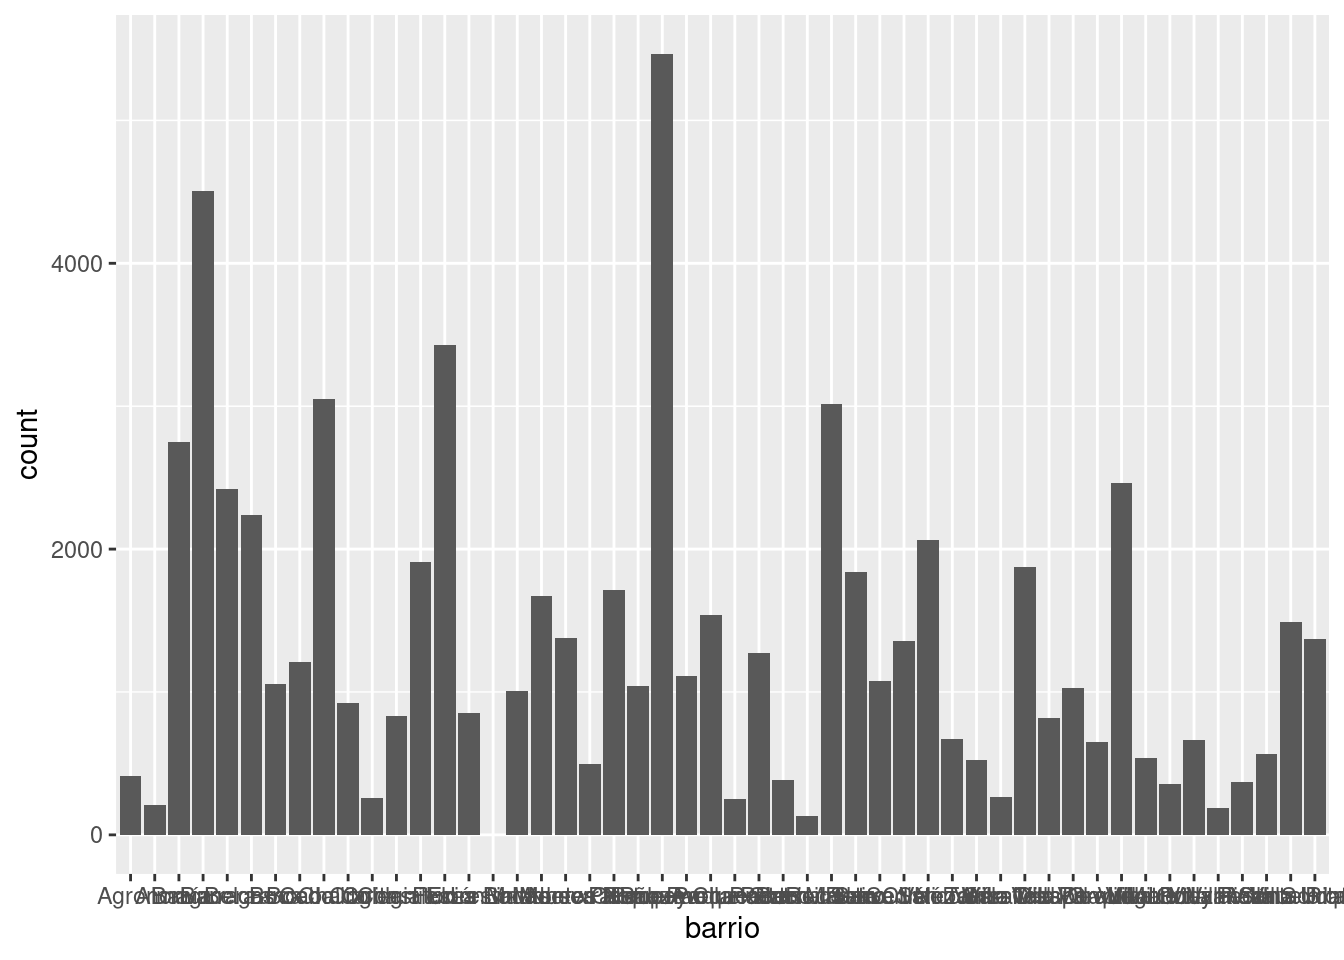
\includegraphics{CD_AJ_files/figure-latex/unnamed-chunk-103-1.pdf}

Tenemos un problema. Los nombres de los barrios resultan ilegibles, porque no tienen espacio suficiente para evitar que aparezcan superpuestos. En un gráfico, el eje horizontal es un muy mal lugar para poner muchas categorías con nombre, ya que el solapamiento se vuelve inevitable. Sería mejor tener los nombre en el eje vertical, donde se pueden escribir uno encima del otro sin pisarse ¡La solución es invertir los ejes de de coordenadas! Sólo necesitamos agregar \texttt{coord\_flip}:

\begin{Shaded}
\begin{Highlighting}[]
\FunctionTok{ggplot}\NormalTok{(delitos) }\SpecialCharTok{+}
    \FunctionTok{geom\_bar}\NormalTok{(}\FunctionTok{aes}\NormalTok{(}\AttributeTok{x =}\NormalTok{ barrio, }\AttributeTok{weight =}\NormalTok{ total)) }\SpecialCharTok{+}
    \FunctionTok{coord\_flip}\NormalTok{()}
\end{Highlighting}
\end{Shaded}

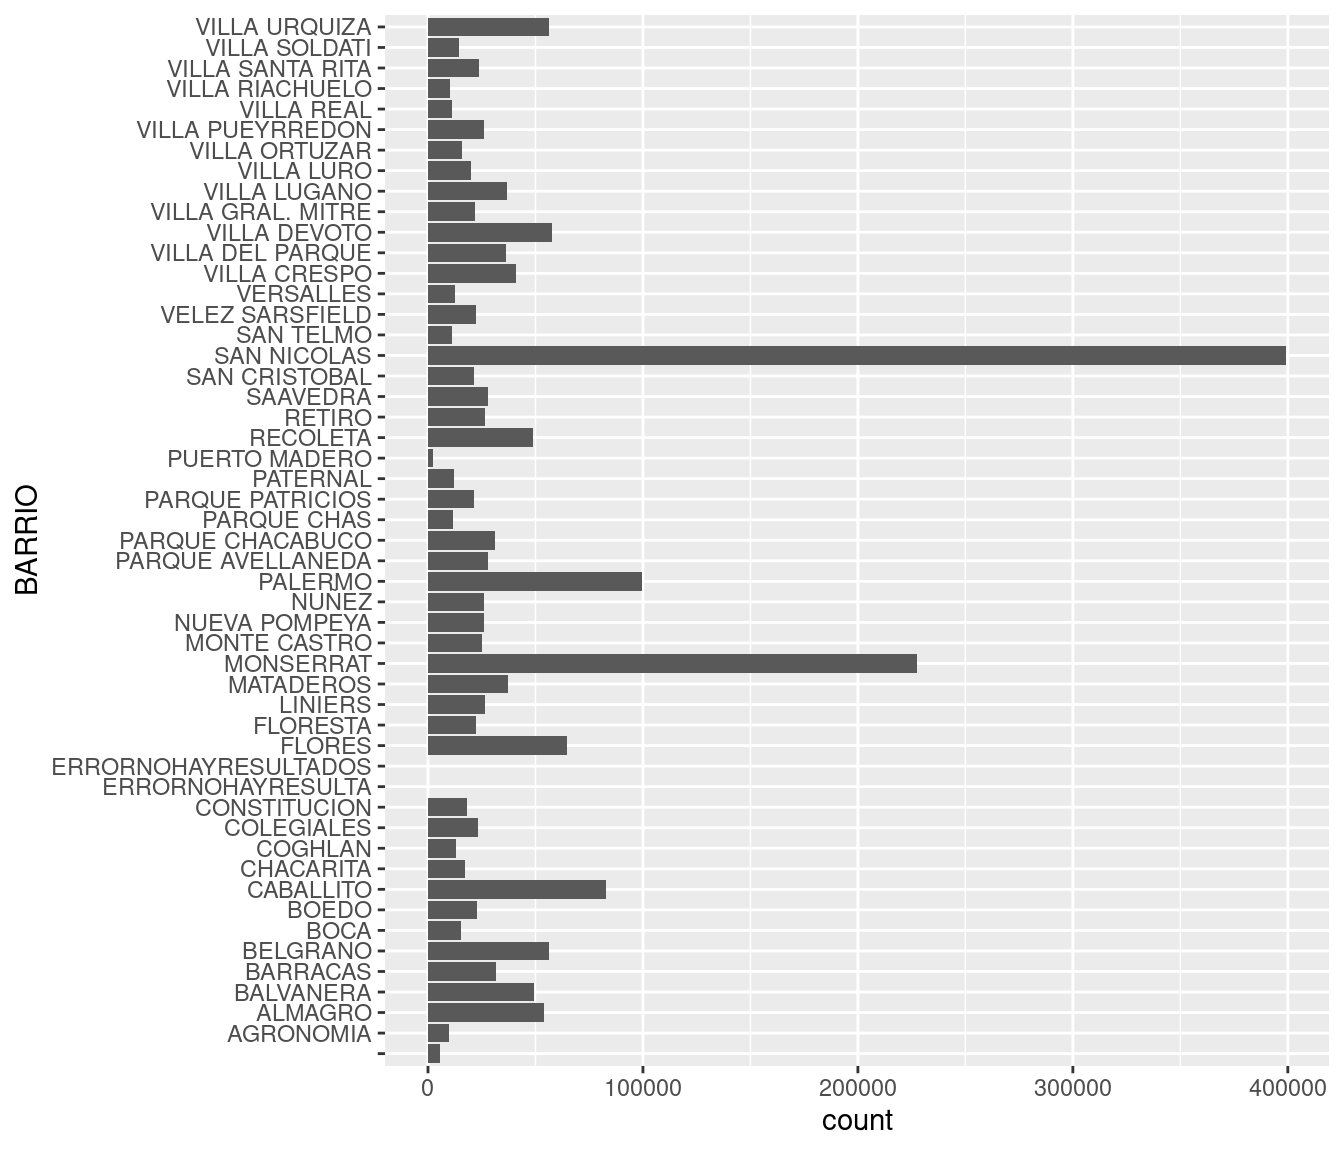
\includegraphics{CD_AJ_files/figure-latex/unnamed-chunk-104-1.pdf}

Ahora si podemos interpretar el gráfico. Además de identificar los barrios que acumulan más registros, este gráfico muestra una situación curiosa, que hasta podría indicar un error en la fuente de datos: en el barrio de La Boca aparentemente no han ocurrido delitos dignos de aparecer en el dataset.

Los gráficos de barras, además de comparar, también son buenos para mostrar la composición interna de las cosas: que ``hay dentro'', que componentes contribuye a un determinado total. Vamos a mostrar entonces cuanto contribuye cada tipo de trámite al total por barrio, usando el parámetro estético \texttt{fill} (relleno). \texttt{geom\_bar} realiza un segmentado automático de cada barra, con la proporción que le corresponde a cada subcategoría:

\begin{Shaded}
\begin{Highlighting}[]
\FunctionTok{ggplot}\NormalTok{(delitos) }\SpecialCharTok{+}
    \FunctionTok{geom\_bar}\NormalTok{(}\FunctionTok{aes}\NormalTok{(}\AttributeTok{x =}\NormalTok{ barrio, }\AttributeTok{weight =}\NormalTok{ total, }\AttributeTok{fill =}\NormalTok{ tipo)) }\SpecialCharTok{+}
    \FunctionTok{coord\_flip}\NormalTok{()}
\end{Highlighting}
\end{Shaded}

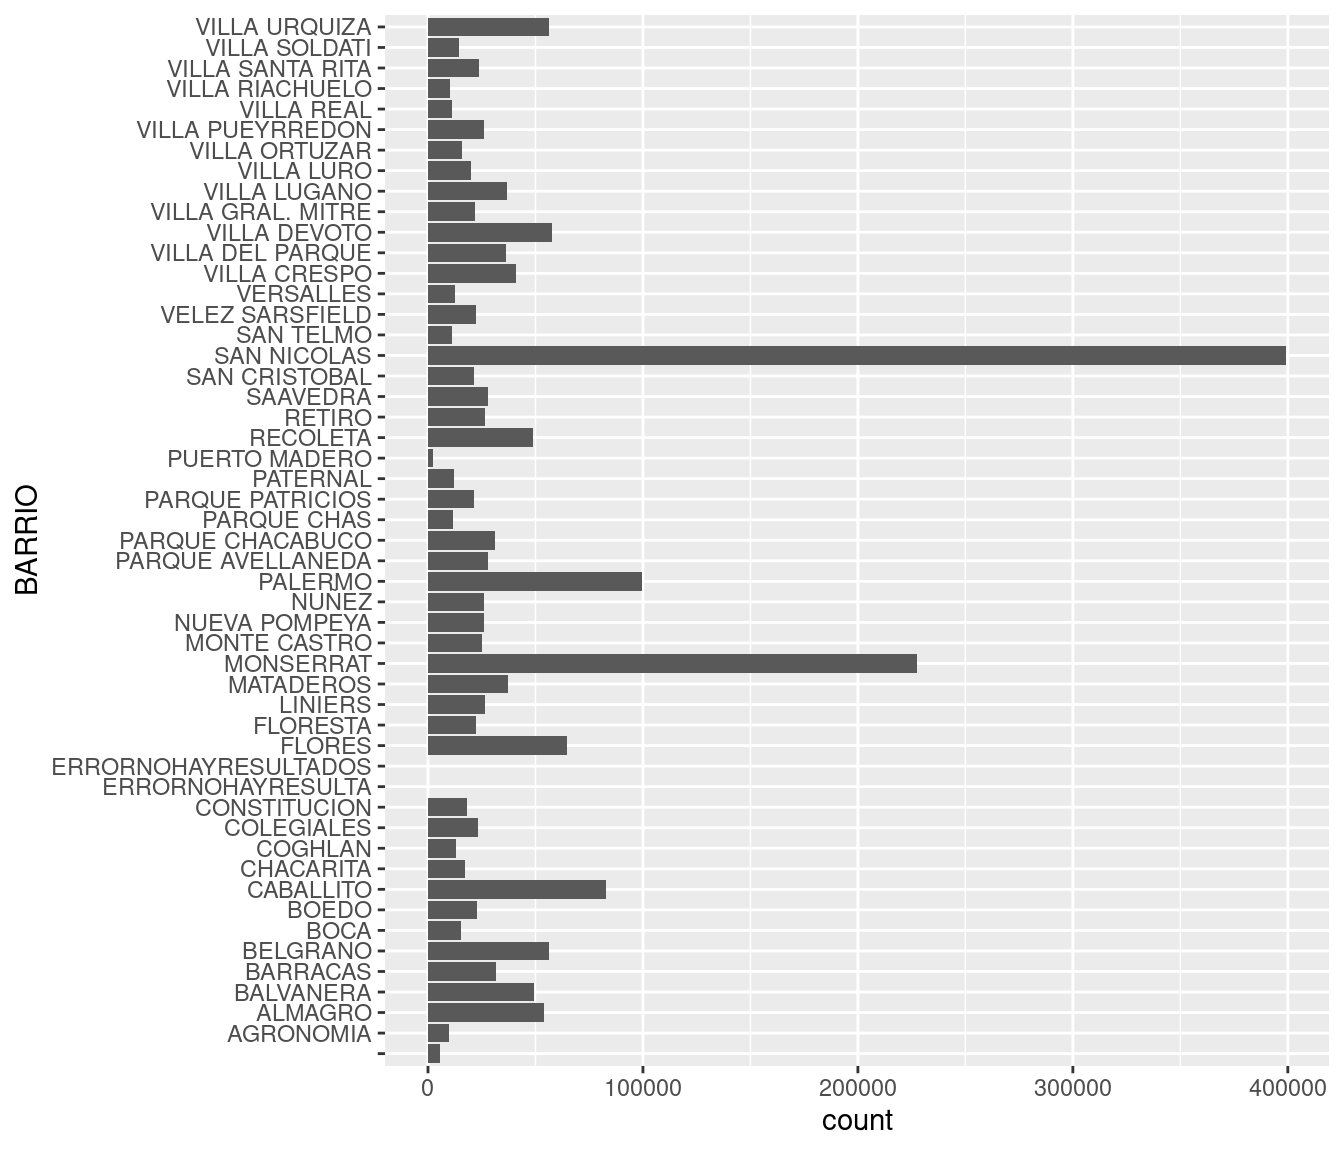
\includegraphics{CD_AJ_files/figure-latex/unnamed-chunk-105-1.pdf}

Ahora se ve que robo y hurto son los tipos más frecuentes, en todos los barrios.

En lugar de relleno podríamos haber usado \texttt{color}, tal como hicimos con los puntos, pero los resultado es un poco menos legible y no luce tan bien. La variable \texttt{color} modifica la silueta de las barras, pero no su interior:

\begin{Shaded}
\begin{Highlighting}[]
\FunctionTok{ggplot}\NormalTok{(delitos) }\SpecialCharTok{+}
    \FunctionTok{geom\_bar}\NormalTok{(}\FunctionTok{aes}\NormalTok{(}\AttributeTok{x =}\NormalTok{ barrio, }\AttributeTok{weight =}\NormalTok{ total, }\AttributeTok{color =}\NormalTok{ tipo)) }\SpecialCharTok{+}
    \FunctionTok{coord\_flip}\NormalTok{()}
\end{Highlighting}
\end{Shaded}

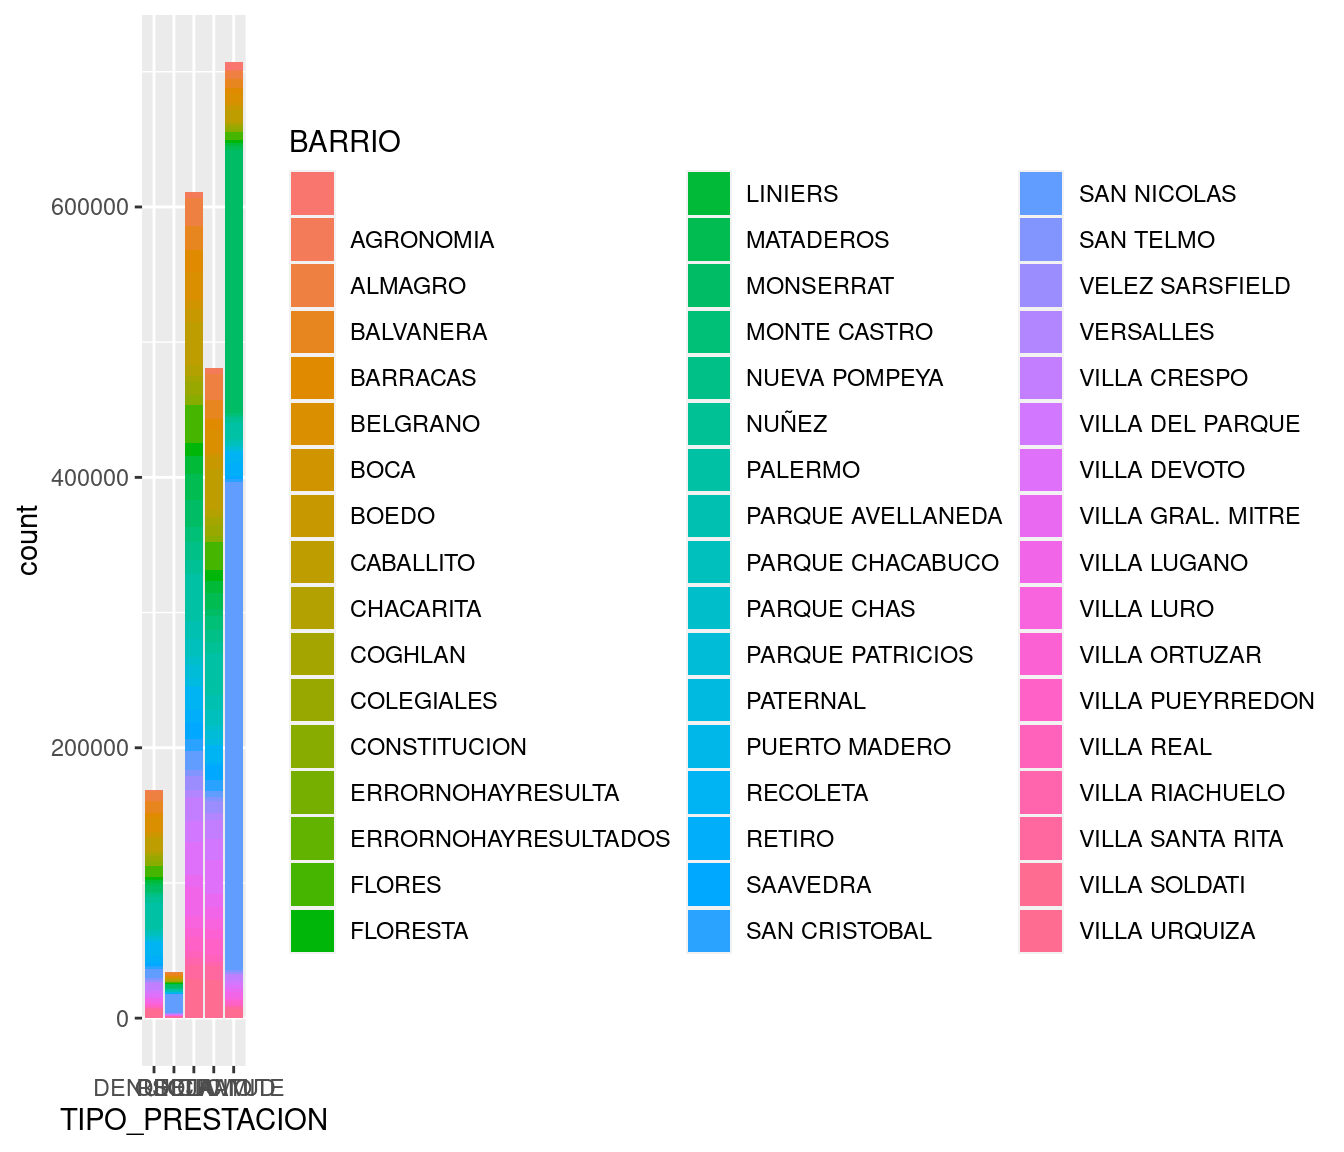
\includegraphics{CD_AJ_files/figure-latex/unnamed-chunk-106-1.pdf}

También podemos dejar de lado los barrios, y concentrarnos en las categorías. Si quisiéramos ver el total de registros por cada sub-tipo de incidente:

\begin{Shaded}
\begin{Highlighting}[]
\FunctionTok{ggplot}\NormalTok{(delitos) }\SpecialCharTok{+}
    \FunctionTok{geom\_bar}\NormalTok{(}\FunctionTok{aes}\NormalTok{(}\AttributeTok{x =}\NormalTok{ tipo, }\AttributeTok{weight =}\NormalTok{ total)) }
\end{Highlighting}
\end{Shaded}

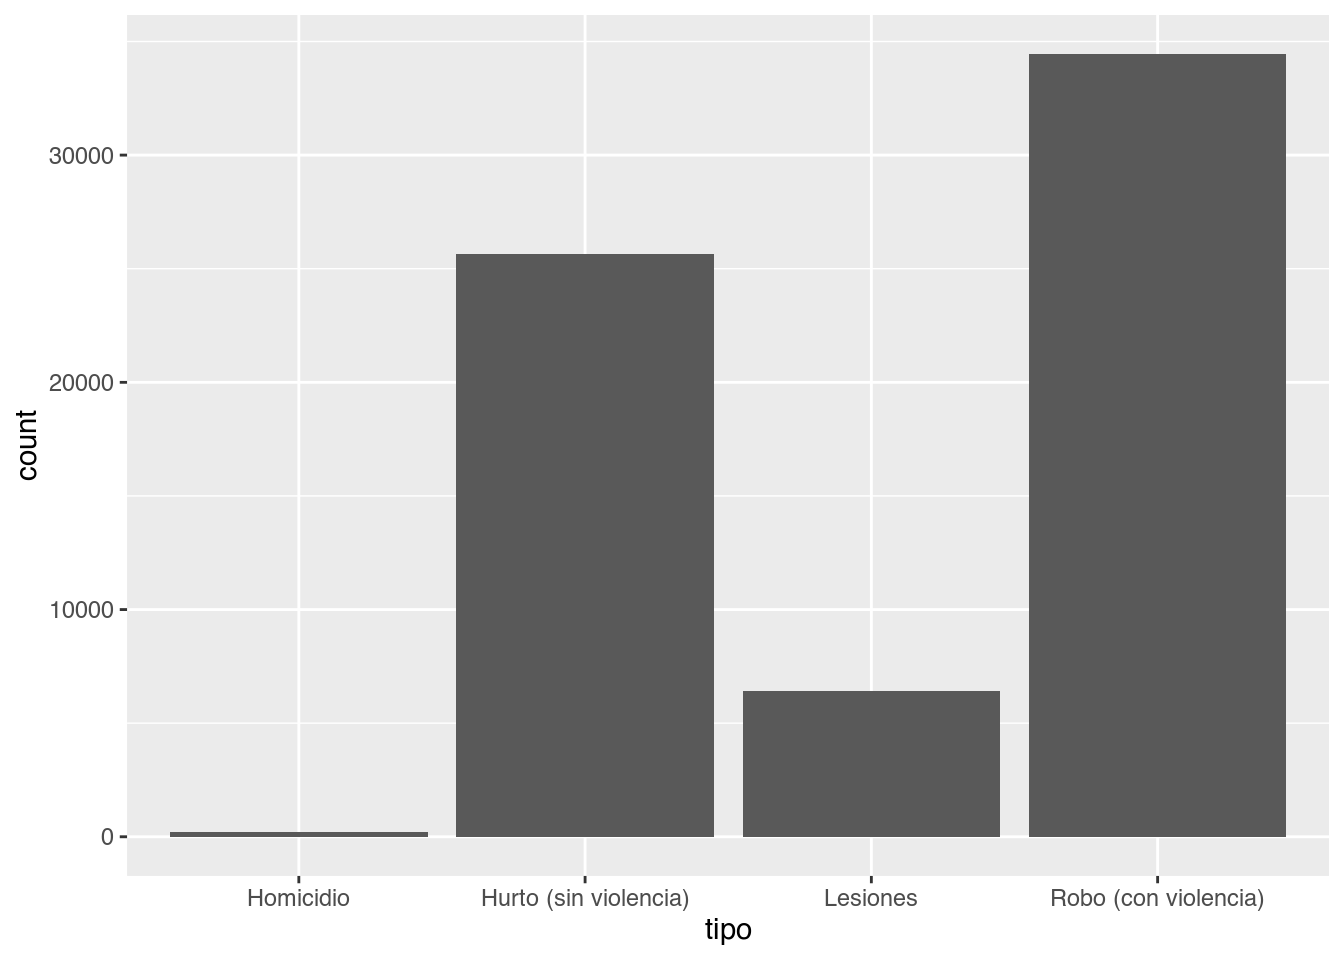
\includegraphics{CD_AJ_files/figure-latex/unnamed-chunk-107-1.pdf}

Notamos que los homicidios y lesiones son eventos poco frecuentes en comparación con las otras clases. En esta ocasión no recurrimos a \texttt{coord\_flip}, ya que las categorías son pocas y tienen espacio suficiente en el eje horizontal.

¿Y si mostramos el aporte de cada barrio al total global de cada tipo de incidente?

\begin{Shaded}
\begin{Highlighting}[]
\FunctionTok{ggplot}\NormalTok{(delitos) }\SpecialCharTok{+}
    \FunctionTok{geom\_bar}\NormalTok{(}\FunctionTok{aes}\NormalTok{(}\AttributeTok{x =}\NormalTok{ tipo, }\AttributeTok{weight =}\NormalTok{ total, }\AttributeTok{fill =}\NormalTok{ barrio)) }
\end{Highlighting}
\end{Shaded}

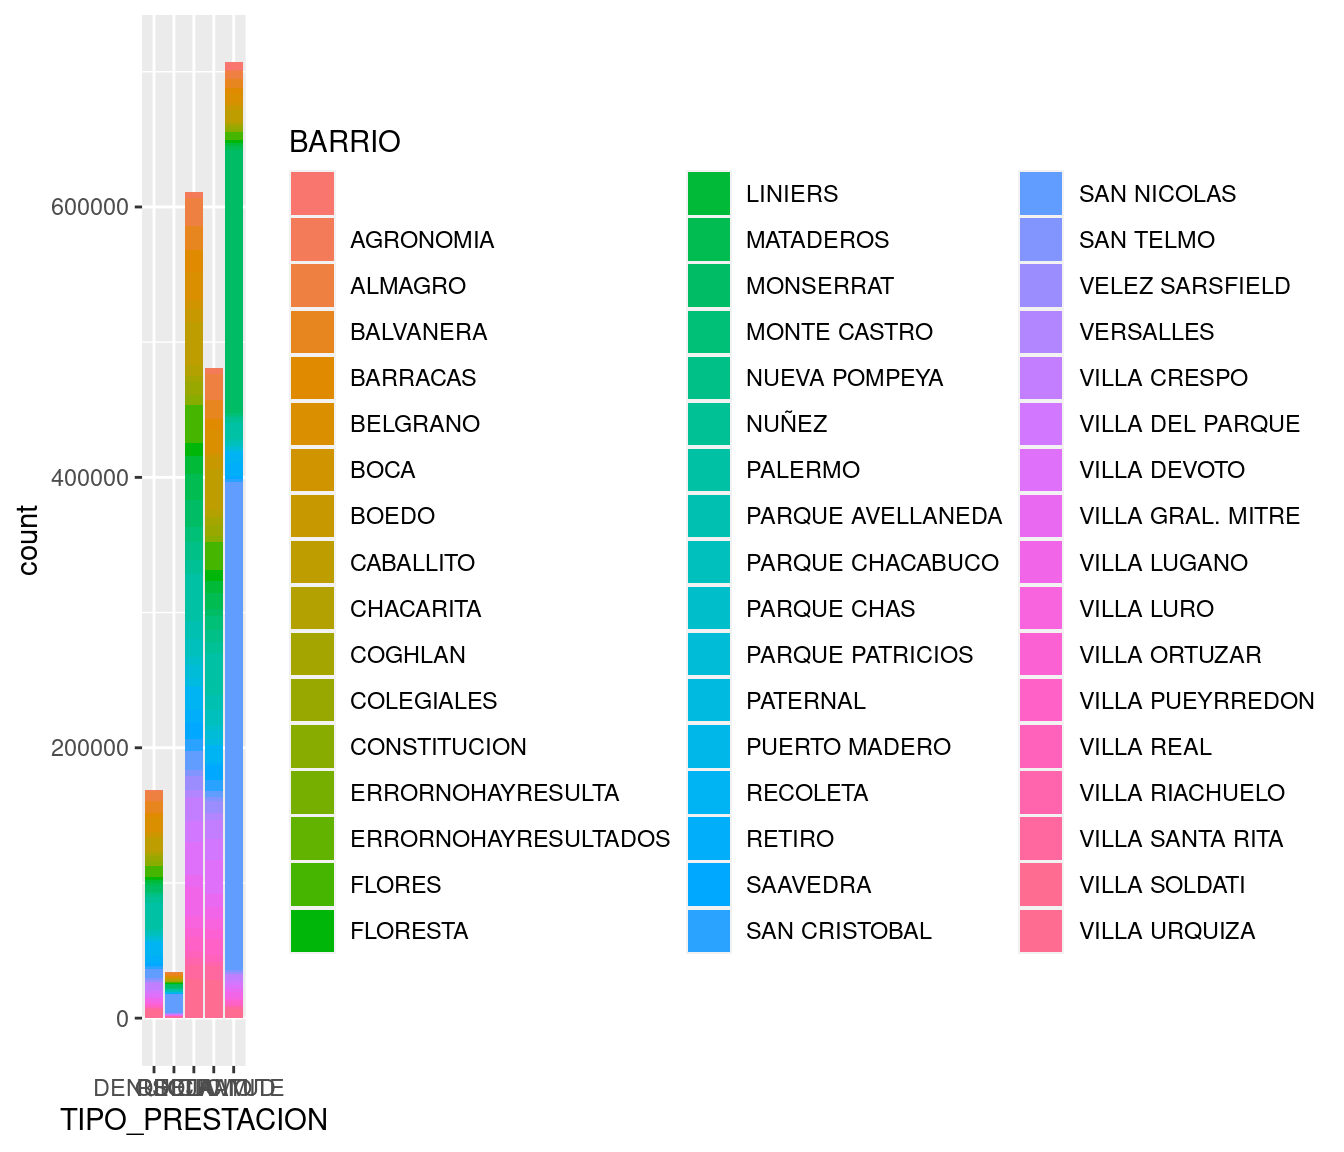
\includegraphics{CD_AJ_files/figure-latex/unnamed-chunk-108-1.pdf}

Hemos obtenido una visualización indigerible. ¡Son demasiadas categorías como para diferenciarlas por color!

Quizás con un facetado por barrio\ldots{}

\begin{Shaded}
\begin{Highlighting}[]
\FunctionTok{ggplot}\NormalTok{(delitos) }\SpecialCharTok{+}
    \FunctionTok{geom\_bar}\NormalTok{(}\FunctionTok{aes}\NormalTok{(}\AttributeTok{x =}\NormalTok{ tipo, }\AttributeTok{weight =}\NormalTok{ total)) }\SpecialCharTok{+}
    \FunctionTok{facet\_wrap}\NormalTok{(}\SpecialCharTok{\textasciitilde{}}\NormalTok{barrio)}
\end{Highlighting}
\end{Shaded}

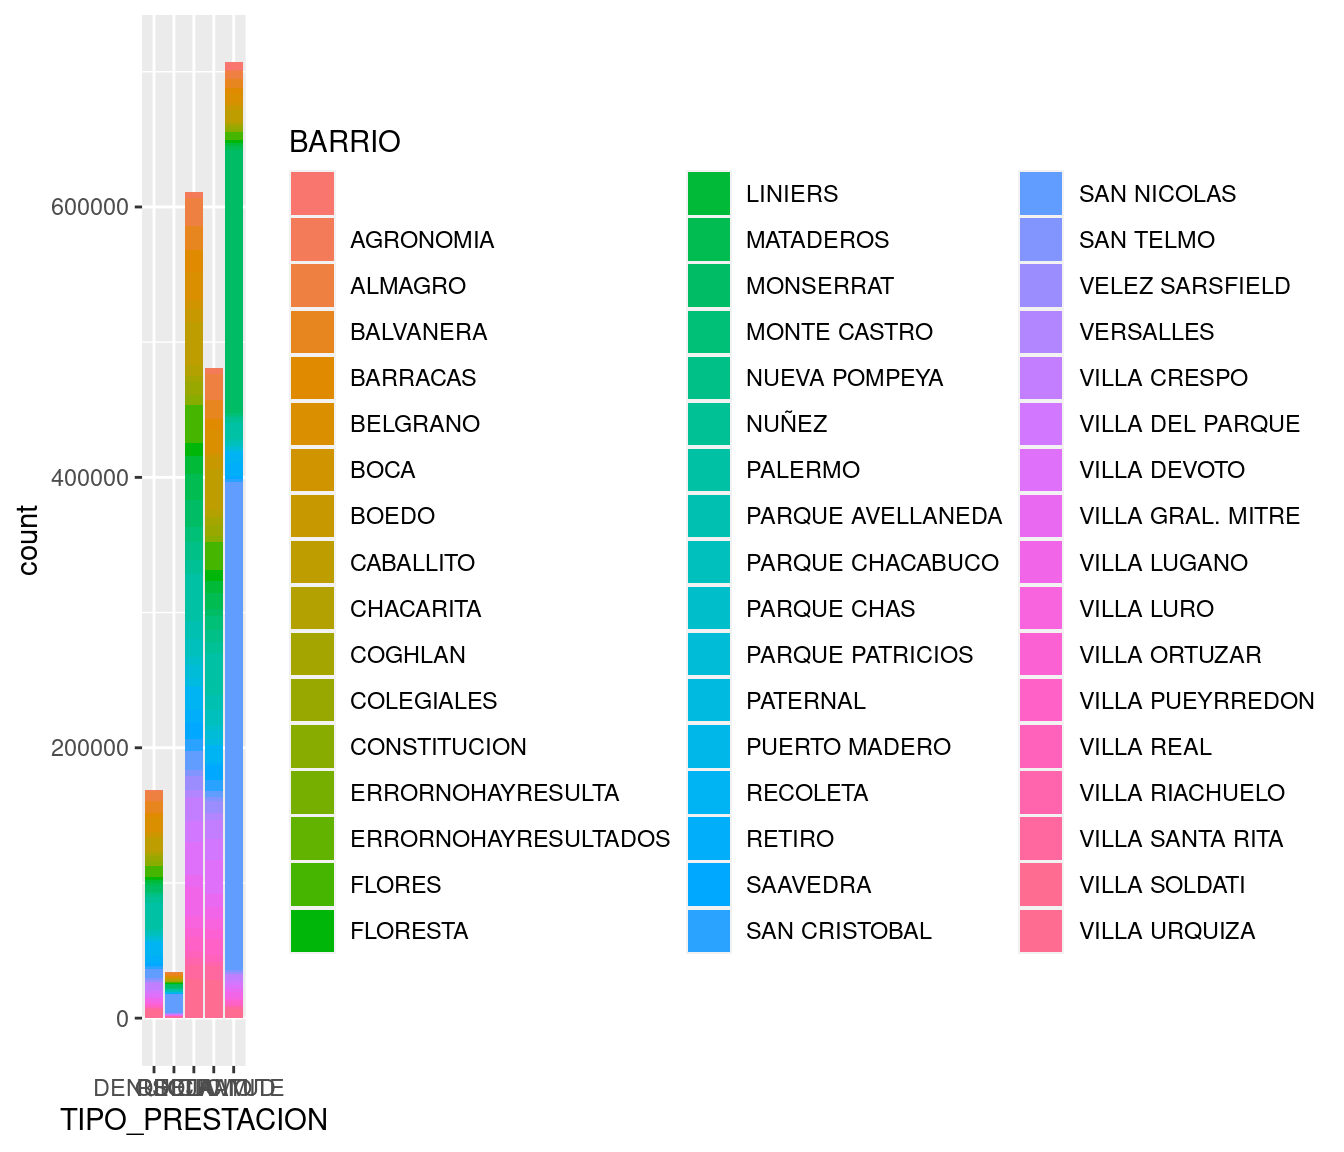
\includegraphics{CD_AJ_files/figure-latex/unnamed-chunk-109-1.pdf}

Esta opción es un poco mejor, ya que al menos permite identificar pronto los barrios salientes, y discernir diferencias generales si se la mira con paciencia. Una visualización tan densa en información puede resultar ideal para ``uso personal'', explorando de forma rápida datos con los que estamos familiarizados, pero es poco recomendable para compartir con otros.

En general, para evitar la confusión asociada a variables con docenas de categorías se busca simplificar definiendo menos grupos. Por ejemplo, como hicimos al comienzo al separar por comunas, que son sólo quince, en lugar de por barrios.

\hypertarget{histogramas}{%
\section{Histogramas}\label{histogramas}}

Los histogramas son usados para mostrar la \emph{distribución} de una variable continua. El histograma permite decir si los valores que toma cada observación se agrupan en torno a un valor ``típico'' o medio -como en el caso de la llamada \emph{distribución normal}-, o en torno a dos valores frecuentes (\emph{distribución bimodal}), o con dispersión sin picos ni valles, donde no hay valores típicos ni atípicos - \emph{distribución uniforme}.

Por ejemplo, veamos la distribución de los barrios respecto a la variable ``cantidad anual de delitos''. Para contabilizar el total de registros por barrio tenemos que agrupar los valores de esa columna, y hacer un resumen (\texttt{summarise()}) que extraiga el gran total:

\begin{Shaded}
\begin{Highlighting}[]
\NormalTok{delitos\_anuales }\OtherTok{\textless{}{-}}\NormalTok{ delitos }\SpecialCharTok{\%\textgreater{}\%} 
    \FunctionTok{group\_by}\NormalTok{(barrio) }\SpecialCharTok{\%\textgreater{}\%} 
    \FunctionTok{summarise}\NormalTok{(}\AttributeTok{gran\_total =} \FunctionTok{sum}\NormalTok{(total))}

\NormalTok{delitos\_anuales}
\end{Highlighting}
\end{Shaded}

\begin{verbatim}
## # A tibble: 50 x 2
##    barrio      gran_total
##    <chr>            <int>
##  1 ""                 411
##  2 "Agronomía"        208
##  3 "Almagro"         2748
##  4 "Balvanera"       4503
##  5 "Barracas"        2422
##  6 "Belgrano"        2238
##  7 "Boca"            1059
##  8 "Boedo"           1213
##  9 "Caballito"       3050
## 10 "Chacarita"        920
## # i 40 more rows
\end{verbatim}

En la tabla de delistos anuales la primera fila tiene vacía la celda de barrio. Esto es porque representa los delitos para los cuales no se conoce el sitio donde ocurrieron. Es decir, muestra el total de delitos encontrados en filas donde la la variable ``barrio'' es \texttt{NA}.

Hacer un histograma es simple con \texttt{geom\_histogram()}: sólo hay que elegir una variable y asignarla a las \texttt{x}.

\begin{Shaded}
\begin{Highlighting}[]
\FunctionTok{ggplot}\NormalTok{(delitos\_anuales) }\SpecialCharTok{+} 
    \FunctionTok{geom\_histogram}\NormalTok{(}\FunctionTok{aes}\NormalTok{(}\AttributeTok{x =}\NormalTok{ gran\_total))}
\end{Highlighting}
\end{Shaded}

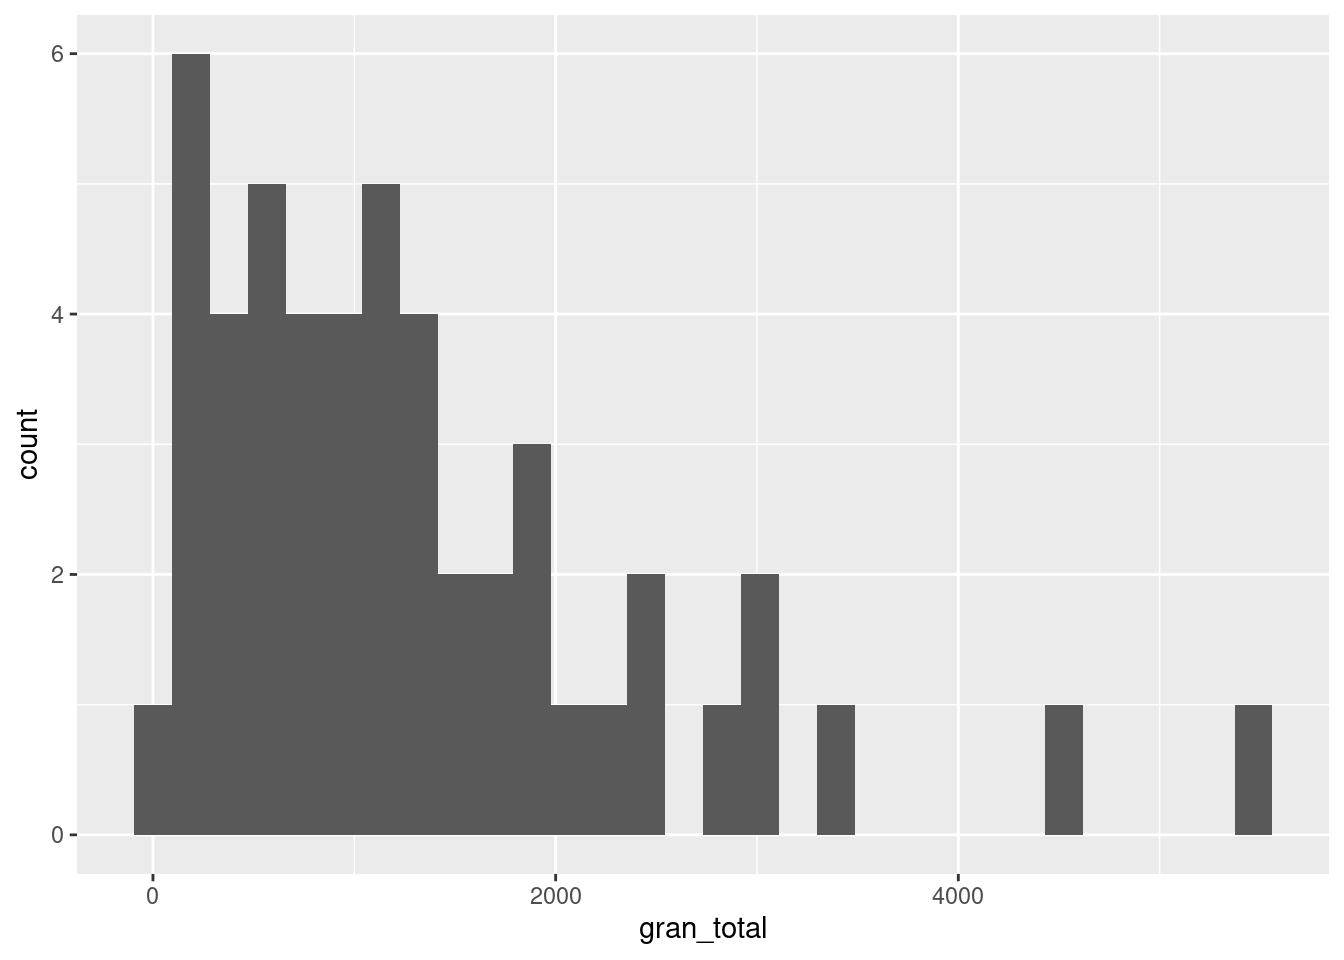
\includegraphics{CD_AJ_files/figure-latex/unnamed-chunk-111-1.pdf}

\texttt{geom\_histogram()} divide el rango de valores en una cantidad arbitraria de segmentos iguales (\emph{bins} en inglés) y cuenta cuántas observaciones caen en cada uno, cantidad que se representa con la altura de la columna en el eje de las \texttt{y}.

En nuestro ejemplo, vemos que la cantidad de registros tiende a agruparse en torno a un valor típico de bastante menos de 1.000 al mes. Aún así, par un par de barrios se contablizaron más de 4.000.

No sería raro que la agregación que hicimos nos oculte patrones en los datos. Que pasa si contamos los registros por mes y por tipo de contacto, y mostramos los histogramas mensuales en facetado por tipo?

Hacemos el agrupado y sumario de rigor,

\begin{Shaded}
\begin{Highlighting}[]
\NormalTok{delitos\_anuales\_por\_tipo }\OtherTok{\textless{}{-}}\NormalTok{ delitos\_anuales }\OtherTok{\textless{}{-}}\NormalTok{ delitos }\SpecialCharTok{\%\textgreater{}\%} 
    \FunctionTok{group\_by}\NormalTok{(barrio, tipo) }\SpecialCharTok{\%\textgreater{}\%} 
    \FunctionTok{summarise}\NormalTok{(}\AttributeTok{gran\_total =} \FunctionTok{sum}\NormalTok{(total))}
\end{Highlighting}
\end{Shaded}

y creamos el facetado como ya sabemos:

\begin{Shaded}
\begin{Highlighting}[]
\FunctionTok{ggplot}\NormalTok{(delitos\_anuales\_por\_tipo) }\SpecialCharTok{+} 
    \FunctionTok{geom\_histogram}\NormalTok{(}\FunctionTok{aes}\NormalTok{(}\AttributeTok{x =}\NormalTok{ gran\_total)) }\SpecialCharTok{+}
    \FunctionTok{facet\_wrap}\NormalTok{(}\SpecialCharTok{\textasciitilde{}}\NormalTok{tipo)}
\end{Highlighting}
\end{Shaded}

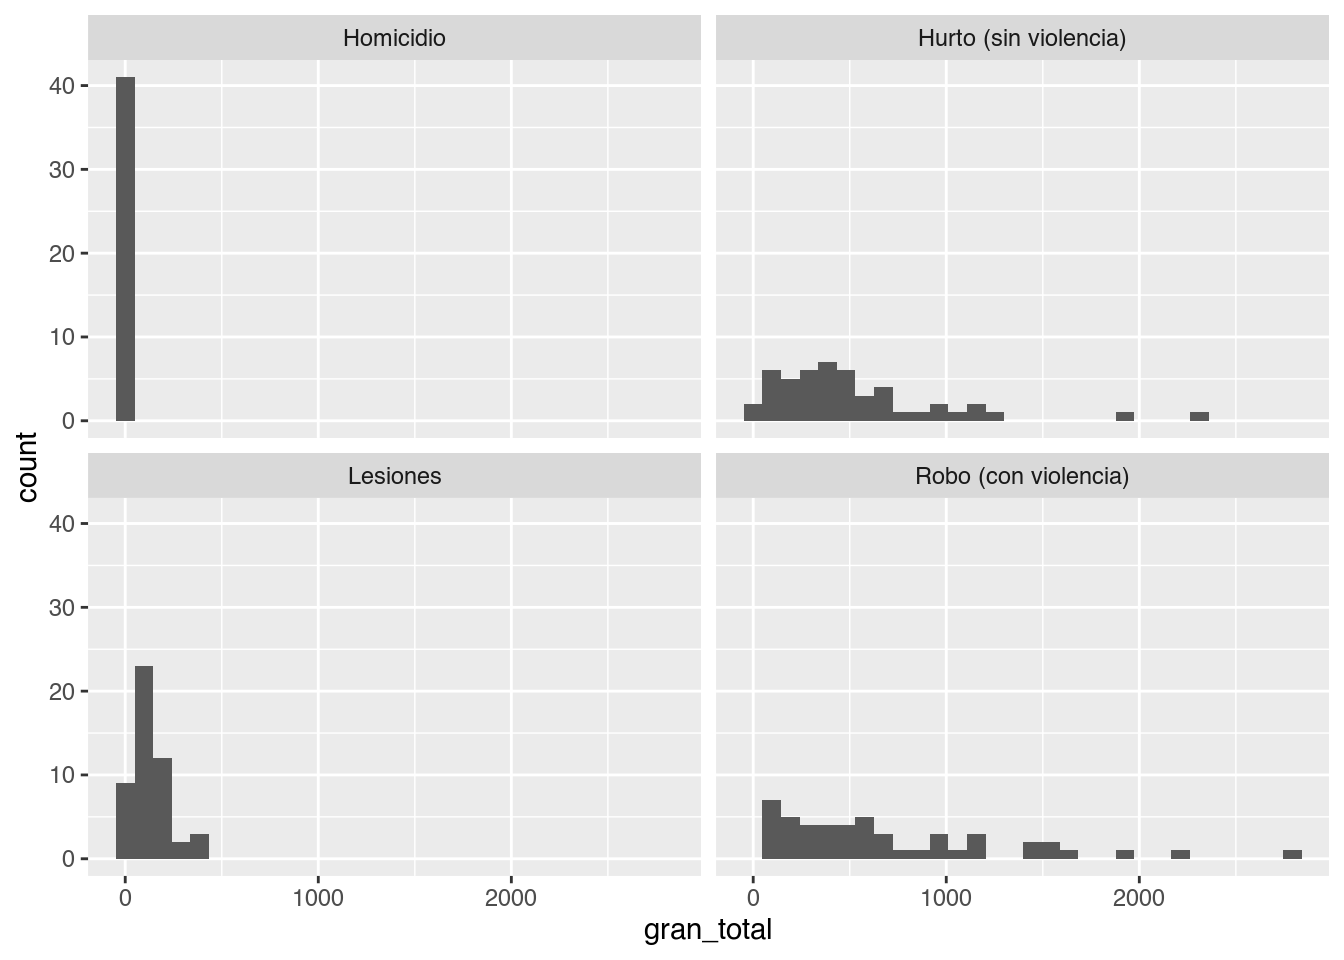
\includegraphics{CD_AJ_files/figure-latex/unnamed-chunk-113-1.pdf}

Aparecen las diferencias. Los homicidios tienen una dispersión mínima, con casi todas las observaciones apiladas en torno a un puñado de casos; siempre son bajas. La cantidad anual de lesiones muestra una dispersión mayor, pero aún así con tendencia a rondar un valor típico. Los hurtos y robos se comportan distinto, ya que muestran una gran dispersión, pudiendo tomar cualquier valor desde una decenas a más de 2.000 registros de forma bastante pareja.

\hypertarget{preparando-una-visualizaciuxf3n-para-compartir}{%
\section{Preparando una visualización para compartir}\label{preparando-una-visualizaciuxf3n-para-compartir}}

Lo último que nos queda por decir en este capítulo es que los gráficos que hemos producido hasta aquí están pensando para nuestro propio consumo. Son parte, y parte fundamental, de lo que llamamos análisis exploratorio de datos. En el contexto de la exploración, lo importante es trabajar en forma rápida, probando una u otra técnica de visualización y refinando nuestros resultados hasta hallar patrones interesantes, o sacarnos dudas acerca de los datos. No necesitamos ponerle título a las visualizaciones, porque ya sabemos de que tratan (¡acabamos de escribirlas!). No nos preocupa que los nombres de los ejes indiquen en forma clara la variable representan, porque ya lo sabemos de antemano.

Pero cuando queremos guardar un gráfico para compartir con otros, sea publicándola en un paper, o enviándola por email a un amigo, necesitamos tener más cuidado. Hemos pasado del ámbito de la exploración al de la comunicación. Ahora si debe preocuparnos la claridad, porque no sabemos el grado de familiaridad que tiene con los datos la eventual audiencia.

Si bien la comunicación clara es un arte cuyas reglas dependen del contexto, y además cada quien tiene su estilo, podemos decretar al menos tres elementos que no deberían faltar en un gráfico destinado a comunicar algo a los demás:

\begin{itemize}
\tightlist
\item
  Un título descriptivo, pero breve
\item
  Etiquetas claras (no ambiguas) en los ejes
\item
  Nombres descriptivos en las leyendas
\end{itemize}

y ya que estamos, dos opcionales:

\begin{itemize}
\tightlist
\item
  Un subtítulo donde poner detalles importantes que no entran en un título breve
\item
  Una nota al pie con información adicional: fuente de los datos, cita académica, advertencias, etc.
\end{itemize}

Con \texttt{ggplot()} podemos encargarnos de todo dentro de una sola función, \texttt{labs()} (por \emph{labels}, etiquetas)

Tomemos un gráfico de los que hicimos antes para pulirlo un poco y que sirva de ejemplo. El original:

\begin{Shaded}
\begin{Highlighting}[]
\FunctionTok{ggplot}\NormalTok{(delitos) }\SpecialCharTok{+}
    \FunctionTok{geom\_bar}\NormalTok{(}\FunctionTok{aes}\NormalTok{(}\AttributeTok{x =}\NormalTok{ barrio, }\AttributeTok{weight =}\NormalTok{ total, }\AttributeTok{fill =}\NormalTok{ tipo)) }\SpecialCharTok{+}
    \FunctionTok{coord\_flip}\NormalTok{()}
\end{Highlighting}
\end{Shaded}

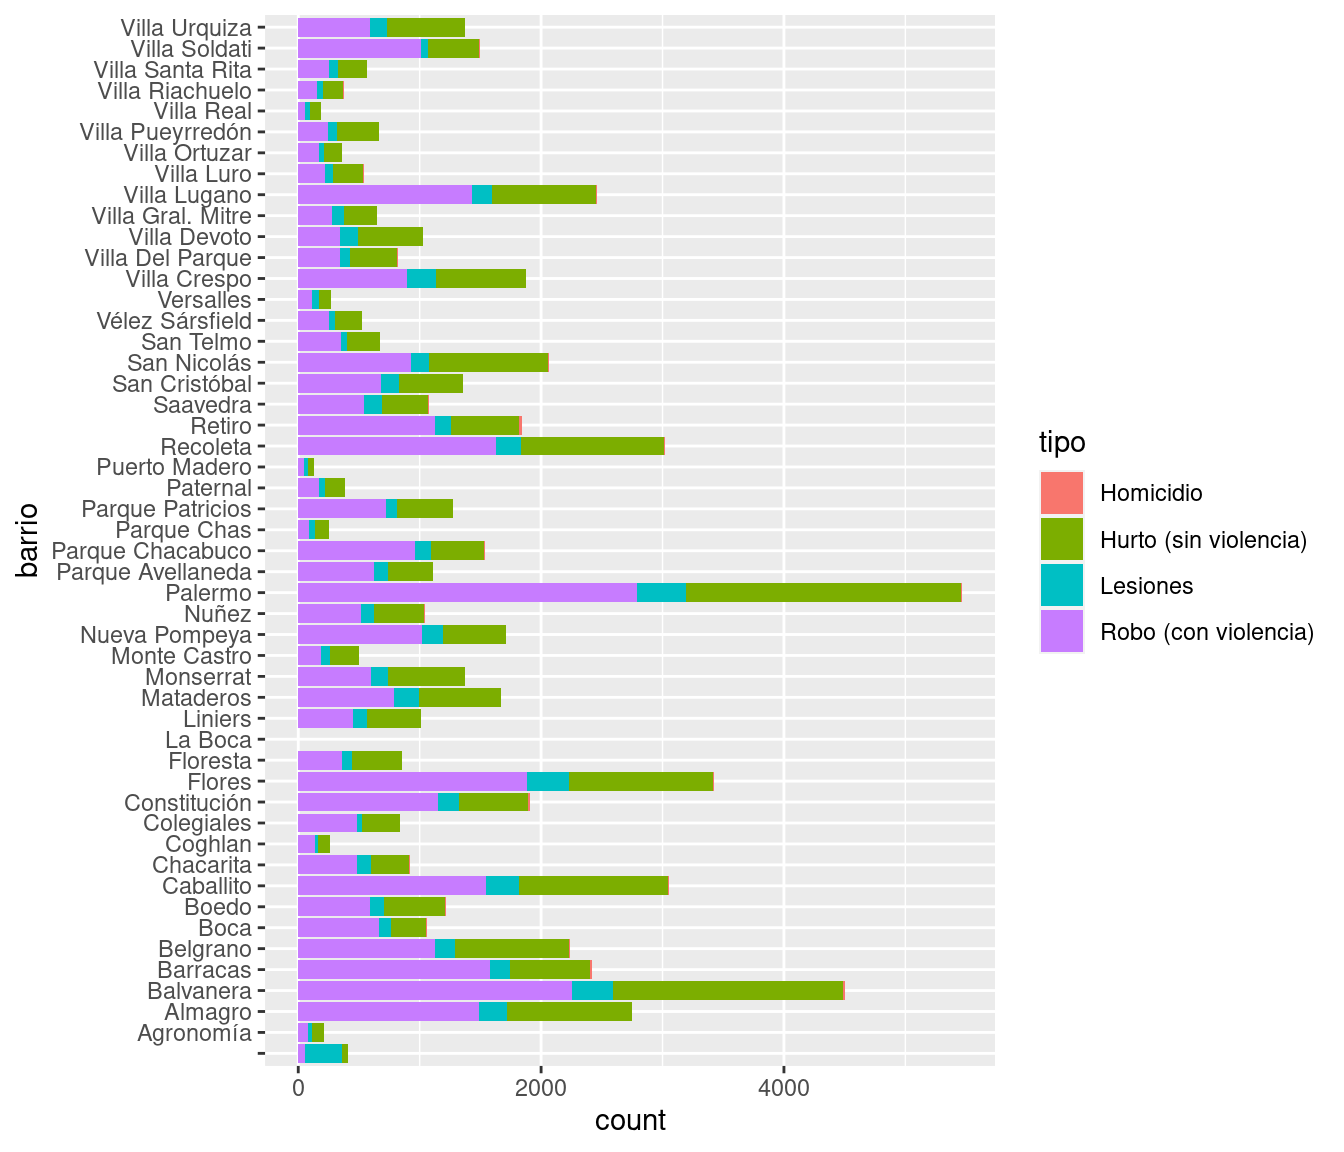
\includegraphics{CD_AJ_files/figure-latex/unnamed-chunk-114-1.pdf}

versus la versión pulida usando \texttt{labs()}:

\begin{Shaded}
\begin{Highlighting}[]
\FunctionTok{ggplot}\NormalTok{(delitos) }\SpecialCharTok{+}
    \FunctionTok{geom\_bar}\NormalTok{(}\FunctionTok{aes}\NormalTok{(}\AttributeTok{x =}\NormalTok{ barrio, }\AttributeTok{weight =}\NormalTok{ total, }\AttributeTok{fill =}\NormalTok{ tipo)) }\SpecialCharTok{+}
    \FunctionTok{coord\_flip}\NormalTok{() }\SpecialCharTok{+}
    \FunctionTok{labs}\NormalTok{(}\AttributeTok{title =} \StringTok{"Delitos registrados"}\NormalTok{,}
         \AttributeTok{subtitle =} \StringTok{"Ciudad Autónoma de Buenos Aires, 2020"}\NormalTok{,}
         \AttributeTok{caption =} \StringTok{"Fuente: portal de datos abiertos de la Ciudad {-} http://data.buenosaires.gob.ar"}\NormalTok{,}
         \AttributeTok{x =} \StringTok{"barrio"}\NormalTok{,}
         \AttributeTok{y =} \StringTok{"cantidad"}\NormalTok{,}
         \AttributeTok{fill =} \StringTok{"Tipo"}\NormalTok{)}
\end{Highlighting}
\end{Shaded}

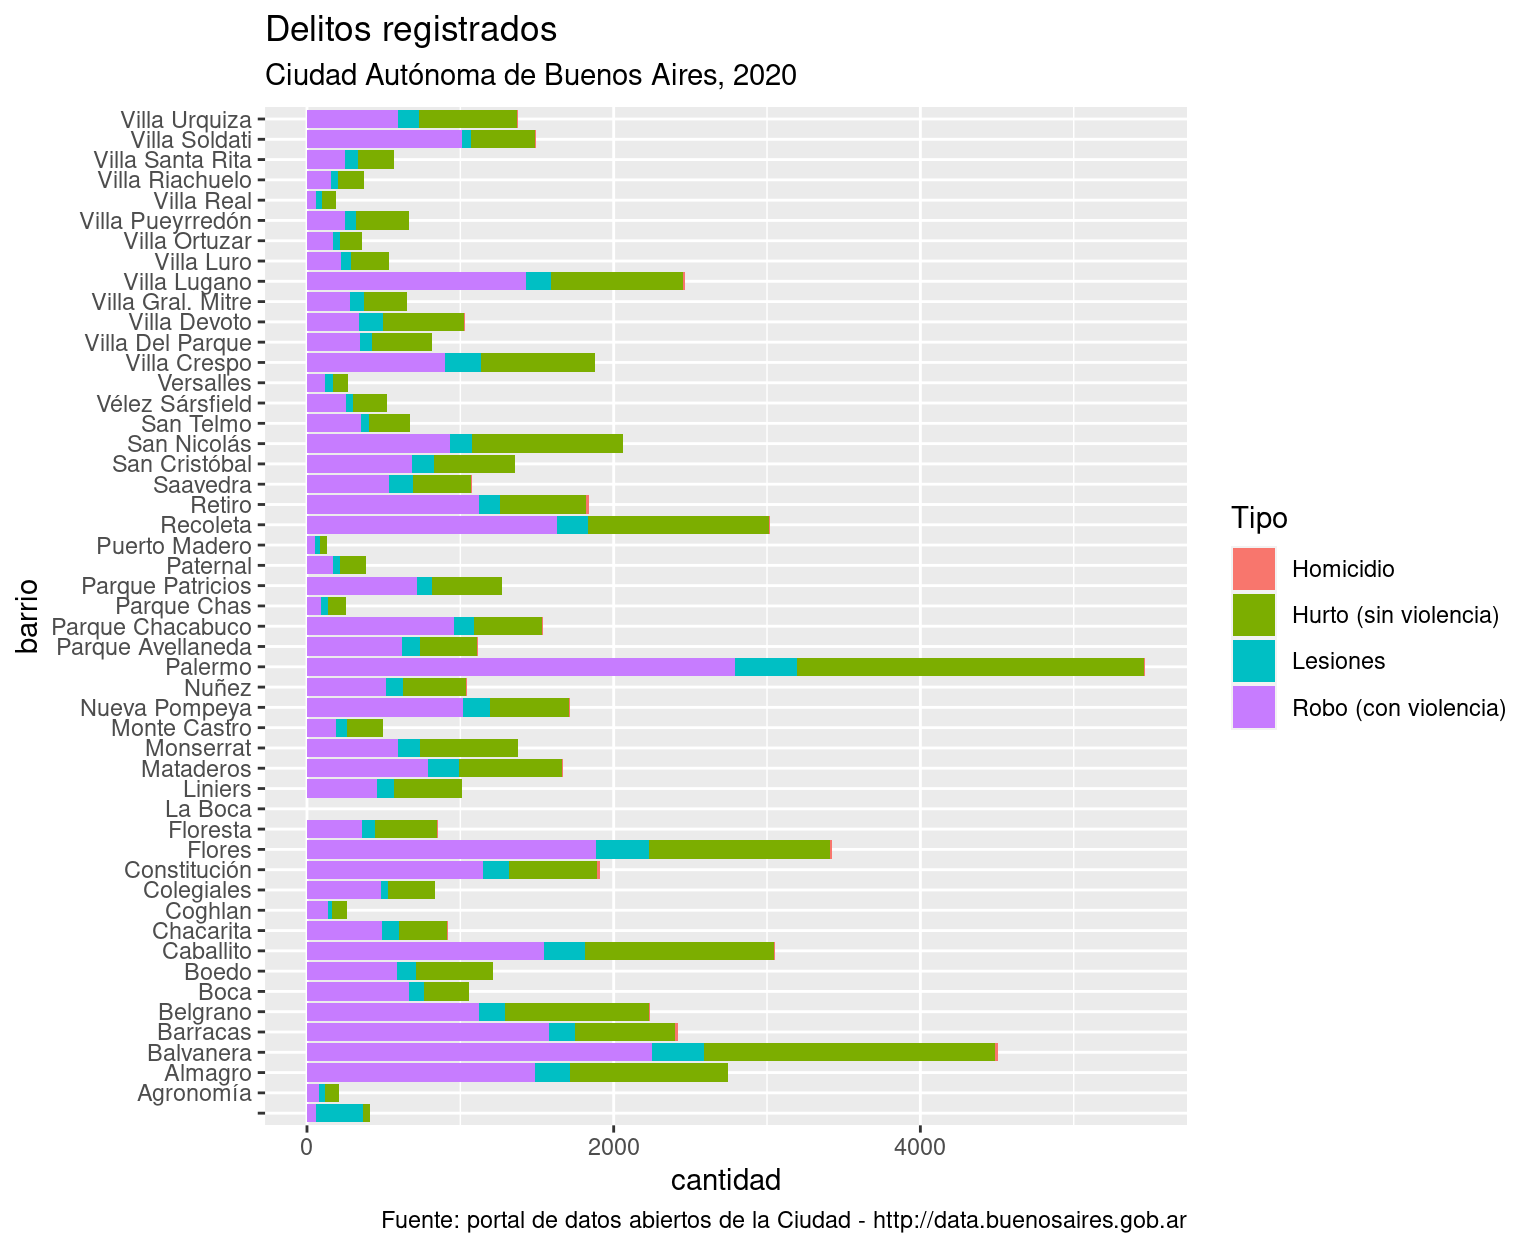
\includegraphics{CD_AJ_files/figure-latex/unnamed-chunk-115-1.pdf}

Ya tiene todo el contenido necesario. Ahora si, a compartir.

En cuanto a la presentación (el aspecto), podríamos hacer un ajuste final que dependerá de nuestros gustos. Los gráficos generados por \texttt{ggplot()} llevan ese panel gris neutro como fondo, que es característico: es fácil reconocer un gráfico hecho con ggplot al verlo en una publicación o sitio web. Sin embargo, nada nos obliga a usar el diseño definido por defecto. Podemos cambiar la tipografía, los colores usados para representar datos, el color de fondo\ldots{} ¡todos y cada uno de los componentes! Una forma sencilla de hacer cambios es aprovechar los ``temas'' (combinaciones de colores) que el paquete \texttt{ggplot2} incluye listos para usar. Para elegir un estilo sólo necesitamos agregar una capa de las que comienza con ``theme\_\ldots{}'', por ejemplo \texttt{theme\_minimal()}, \texttt{theme\_dark()}, \texttt{theme\_classic()}.

En mi experiencia, el que mejor luce en la gran mayoría de los casos es \texttt{theme\_minimal}. Vamos a usarlo, repitiendo el código que generó la última visualización que hicimos, y agregando una línea al final para definir el tema.

\begin{Shaded}
\begin{Highlighting}[]
\FunctionTok{ggplot}\NormalTok{(delitos) }\SpecialCharTok{+}
    \FunctionTok{geom\_bar}\NormalTok{(}\FunctionTok{aes}\NormalTok{(}\AttributeTok{x =}\NormalTok{ barrio, }\AttributeTok{weight =}\NormalTok{ total, }\AttributeTok{fill =}\NormalTok{ tipo)) }\SpecialCharTok{+}
    \FunctionTok{coord\_flip}\NormalTok{() }\SpecialCharTok{+}
    \FunctionTok{labs}\NormalTok{(}\AttributeTok{title =} \StringTok{"Delitos registrados"}\NormalTok{,}
         \AttributeTok{subtitle =} \StringTok{"Ciudad Autónoma de Buenos Aires, 2020"}\NormalTok{,}
         \AttributeTok{caption =} \StringTok{"Fuente: portal de datos abiertos de la Ciudad {-} http://data.buenosaires.gob.ar"}\NormalTok{,}
         \AttributeTok{x =} \StringTok{"barrio"}\NormalTok{,}
         \AttributeTok{y =} \StringTok{"cantidad"}\NormalTok{,}
         \AttributeTok{fill =} \StringTok{"Tipo"}\NormalTok{) }\SpecialCharTok{+}
    \FunctionTok{theme\_minimal}\NormalTok{()}
\end{Highlighting}
\end{Shaded}

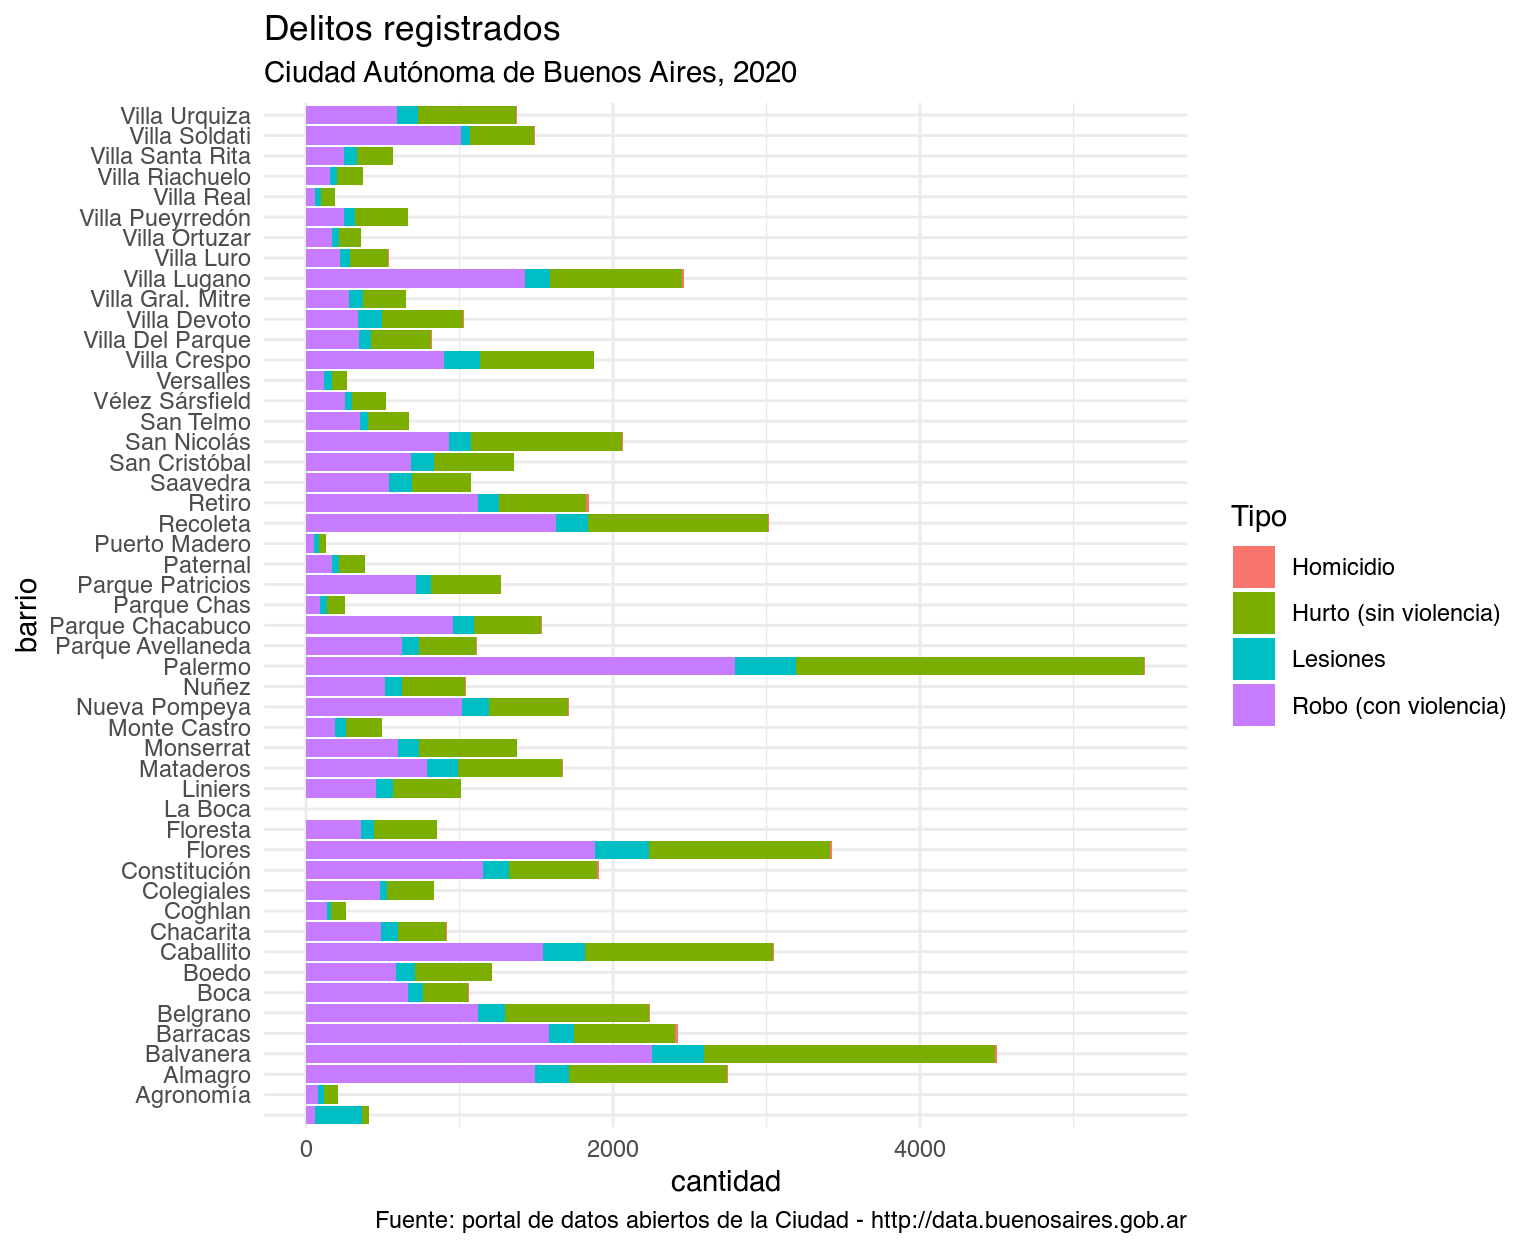
\includegraphics{CD_AJ_files/figure-latex/unnamed-chunk-116-1.pdf}

\ldots no esta mal, ¿verdad?

\hypertarget{otras-visualizaciones}{%
\section{Otras visualizaciones}\label{otras-visualizaciones}}

Por supuesto, las opciones que hemos repasado son apenas una fracción de la enorme variedad de técnicas de visualización que existen. Para empezar, nos falta hablar de los mapas, una categoría tan importante que tiene un capítulo completo dedicado más adelante.

Y aún quedan tantas por discutir, que sería imposible hacerles justicia en un libro introductorio. Con nombres tan variopintos como \emph{waffle charts}, \emph{violin plots}, o \emph{tree maps}, existen quizás un centenar o más de métodos bien documentados para explorar información en forma visual.

El sitio web \emph{from Data to Viz} (\url{https://www.data-to-viz.com/}) es un recurso excelente para investigar opciones. Contiene un compendio visual e interactivo de técnicas de visualización con sus nombres y características generales. También explica a que familia corresponde cada una, y para qué suele usarse (mostrar relaciones, distribuciones, cambio a través del tiempo, etc).

\begin{figure}
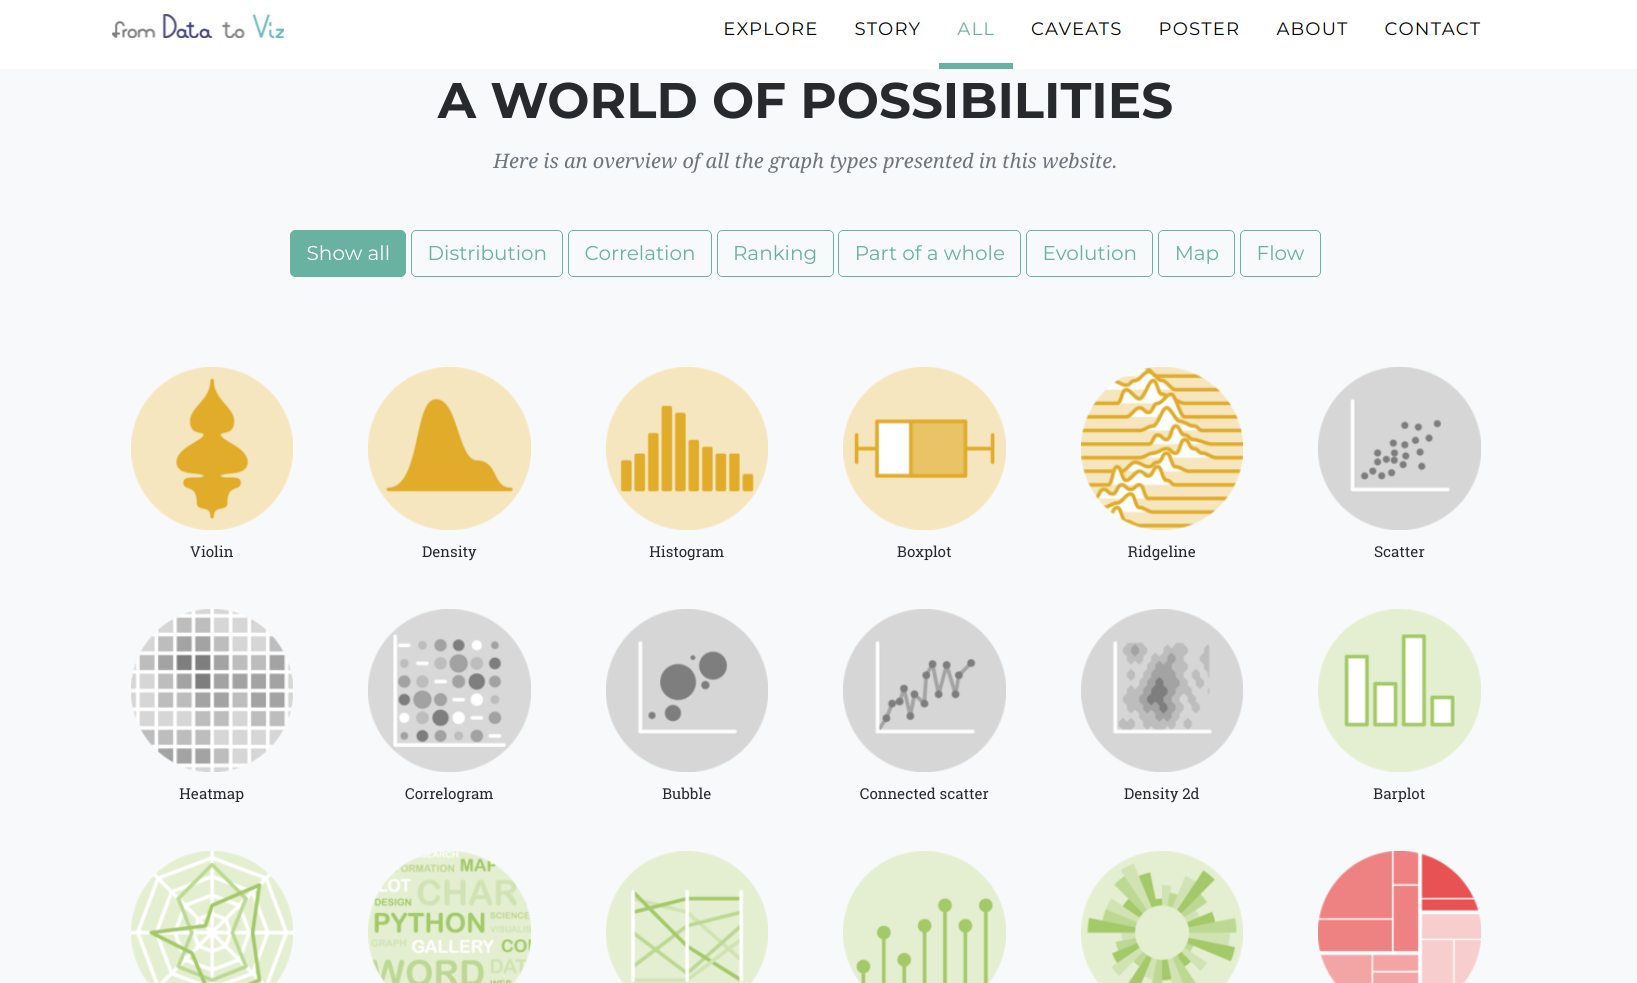
\includegraphics[width=1\linewidth]{imagenes/data_to_viz} \caption{from Data to Viz - www.data-to-viz.com/}\label{fig:unnamed-chunk-117}
\end{figure}

Y lo más interesante: Para todas y cada una de las visualizaciones se incluye el código en R que permite reproducirlas. A partir de allí sólo es cuestión de adaptar los ejemplos a nuestros datos para realizar de forma fácil la visualización que nos interesa.

\hypertarget{ejercicios-2}{%
\section{Ejercicios}\label{ejercicios-2}}

I. Tomemos un dataset, y efectuemos las transformaciones necesarias para luego crear las siguientes visualizaciones:

\begin{itemize}
\tightlist
\item
  \emph{Scatter plot}, o gráfico de dispersión: Mostrar correlación entre 2 variables numéricas.
\item
  Gráfico de Barras: Comparar variables categóricas.
\item
  Gráfico de Barras: Comparar variables categóricas mostrando la composición interna de las mismas.\\
\item
  Histograma: Mostrar la distribución de una variable continua.
\end{itemize}

\begin{enumerate}
\def\labelenumi{\Roman{enumi}.}
\setcounter{enumi}{1}
\item
  Realicemos una versión facetada (con \texttt{facet\_wrap()}) de cada tipo de gráfico.
\item
  Pongamos a cada visualización su título, subtítulo, etiquetas en los ejes, nombre descriptivo en la leyenda y nota al pie.
\end{enumerate}

\hypertarget{analisis-de-texto}{%
\chapter{Analisis de texto}\label{analisis-de-texto}}

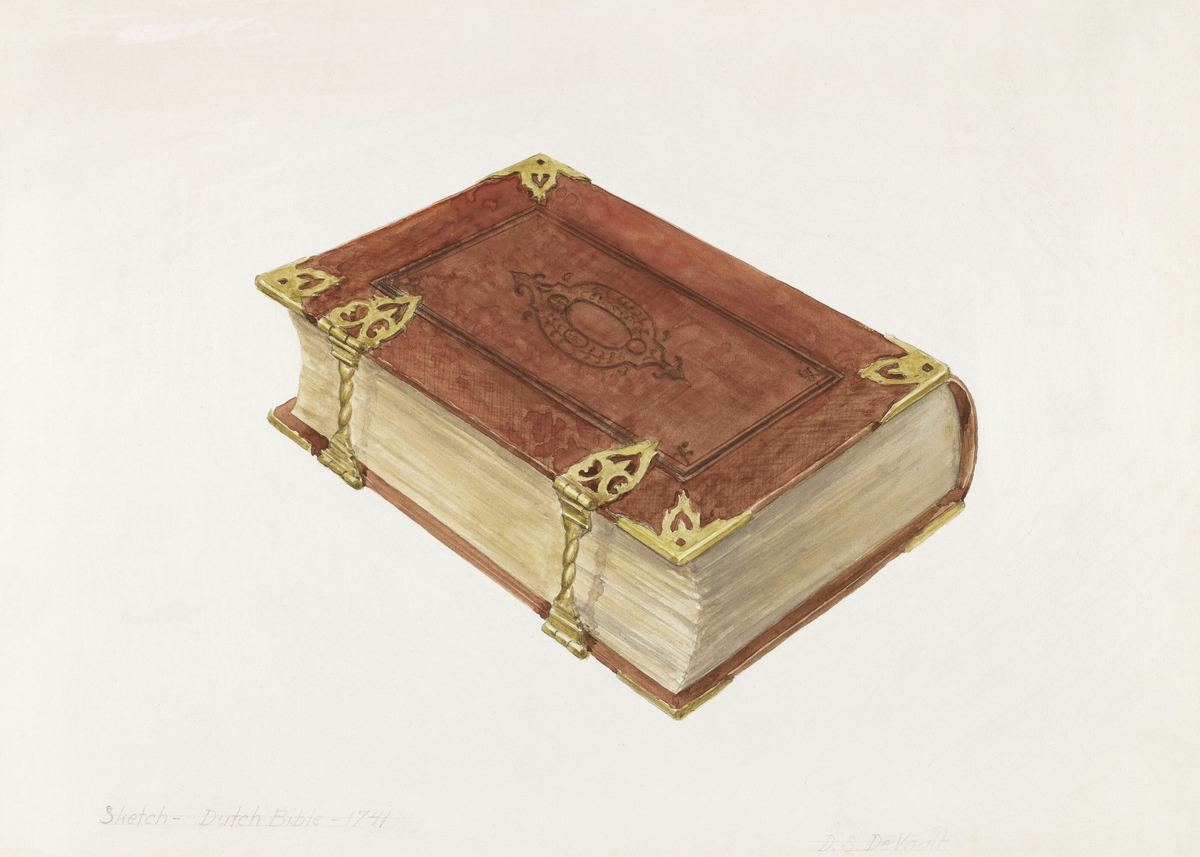
\includegraphics[width=1\linewidth]{imagenes/textos}

A veces, lo que queremos analizar es un texto. Los textos, audios e imágenes son datos no estructurados y hay que realizar algún tipo de preparación o estructuración para poder procesarlos automáticamente.

En el análisis automático de texto se suelen partir los documentos, y armar lo que se llama un \emph{bolsa de palabras}, donde se rompe la sintaxis . Ello sirve para medir frecuencias de palabras, cercanía entre ellas, clasificarlas como ``positivas'' o ``negativas'' sentimentalmente hablando, etc. La minería de texto tiene diversas herramientas para realizar este tipo de tareas.

Las palabras, por su parte, son cadenas de caracteres, y también se pueden manipular de modo automático. Para hacer ello usaremos lo que se conoce como \emph{expresiones regulares} (``regular expressions'' o regex) que permitirá detectar patrones y manipularlos. Las \texttt{regex} son relativamente antiguas (circa 1950) y tuvieron un desarrollo paralelo a la ciencia de datos. Por ello, vienen en varios sabores, cada uno sutilmente diferente al otro. \texttt{R} utiliza \texttt{regex}a través de varios paquetes, entre ellos el \texttt{stringr} de la constelación \texttt{tidyverse}.

\hypertarget{manipulaciuxf3n-de-texto}{%
\section{Manipulación de texto}\label{manipulaciuxf3n-de-texto}}

En \texttt{stringr} todas las funciones comienza con \texttt{str\_}. Usando RStudio, si se presionamos la tecla \texttt{tab} luego de escribir \texttt{str\_} vamos a ver una lista de funciones sugeridas. Por ejemplo, para unir -o \emph{c}oncatenar- caracteres se utiliza \texttt{str\_c}:

\begin{Shaded}
\begin{Highlighting}[]
\FunctionTok{library}\NormalTok{(tidyverse)}
\NormalTok{oracion }\OtherTok{\textless{}{-}} \FunctionTok{c}\NormalTok{(}\StringTok{"Esta"}\NormalTok{, }\StringTok{"es"}\NormalTok{, }\StringTok{"una"}\NormalTok{, }\StringTok{"cadena"}\NormalTok{, }\StringTok{"de"}\NormalTok{, }\StringTok{"palabras."}\NormalTok{)}
\NormalTok{oracion}
\end{Highlighting}
\end{Shaded}

\begin{verbatim}
## [1] "Esta"      "es"        "una"       "cadena"    "de"        "palabras."
\end{verbatim}

\begin{Shaded}
\begin{Highlighting}[]
\CommentTok{\# con \textasciigrave{}collapse = " "\textasciigrave{} indicamos que queremos combinar los elementos y separarlos con un espacio}
\NormalTok{oracion }\OtherTok{\textless{}{-}} \FunctionTok{str\_c}\NormalTok{(oracion, }\AttributeTok{collapse =} \StringTok{" "}\NormalTok{) }
\NormalTok{oracion}
\end{Highlighting}
\end{Shaded}

\begin{verbatim}
## [1] "Esta es una cadena de palabras."
\end{verbatim}

Para extraer caracteres de una palabra se utiliza \texttt{str\_sub}. Hay que señalar el comienzo y el final de lo que se quiera extraer, con el número de la posición:

\begin{Shaded}
\begin{Highlighting}[]
\NormalTok{frutas }\OtherTok{\textless{}{-}} \FunctionTok{c}\NormalTok{(}\StringTok{"Manzana"}\NormalTok{, }\StringTok{"Banana"}\NormalTok{, }\StringTok{"Pera"}\NormalTok{)}
\FunctionTok{str\_sub}\NormalTok{(frutas, }\DecValTok{1}\NormalTok{, }\DecValTok{3}\NormalTok{)}
\end{Highlighting}
\end{Shaded}

\begin{verbatim}
## [1] "Man" "Ban" "Per"
\end{verbatim}

\begin{Shaded}
\begin{Highlighting}[]
\FunctionTok{str\_sub}\NormalTok{(frutas, }\SpecialCharTok{{-}}\DecValTok{3}\NormalTok{, }\SpecialCharTok{{-}}\DecValTok{1}\NormalTok{)}
\end{Highlighting}
\end{Shaded}

\begin{verbatim}
## [1] "ana" "ana" "era"
\end{verbatim}

Se puede pasar los caracteres a mayúscula, o a minúscula:

\begin{Shaded}
\begin{Highlighting}[]
\FunctionTok{str\_to\_lower}\NormalTok{(frutas)}
\end{Highlighting}
\end{Shaded}

\begin{verbatim}
## [1] "manzana" "banana"  "pera"
\end{verbatim}

\begin{Shaded}
\begin{Highlighting}[]
\FunctionTok{str\_to\_upper}\NormalTok{(frutas)}
\end{Highlighting}
\end{Shaded}

\begin{verbatim}
## [1] "MANZANA" "BANANA"  "PERA"
\end{verbatim}

\begin{Shaded}
\begin{Highlighting}[]
\FunctionTok{str\_to\_sentence}\NormalTok{(}\FunctionTok{str\_c}\NormalTok{(frutas, }\AttributeTok{collapse =} \StringTok{" "}\NormalTok{))}
\end{Highlighting}
\end{Shaded}

\begin{verbatim}
## [1] "Manzana banana pera"
\end{verbatim}

Una función muy importante nos permite detectar patrones, \texttt{str\_detect}, que nos dice si es verdadero o falso que dicho patrón está en el objeto. Para verlo más en detalle, utilizaremos \texttt{str\_view} para que la señale en el texto cuando la detecte:

\begin{Shaded}
\begin{Highlighting}[]
\NormalTok{frutas}
\end{Highlighting}
\end{Shaded}

\begin{verbatim}
## [1] "Manzana" "Banana"  "Pera"
\end{verbatim}

\begin{Shaded}
\begin{Highlighting}[]
\FunctionTok{str\_view}\NormalTok{(frutas, }\StringTok{"an"}\NormalTok{)}
\end{Highlighting}
\end{Shaded}

\begin{verbatim}
## [1] | M<an>z<an>a
## [2] | B<an><an>a
\end{verbatim}

Y ahora es donde comienzan a ponerse interesantes las \texttt{regex}. Por ejemplo, el punto (.) puede reemplazar a cualquie caracter, excepto el salto de línea

\begin{Shaded}
\begin{Highlighting}[]
\FunctionTok{str\_view}\NormalTok{(frutas, }\StringTok{".an"}\NormalTok{)}
\end{Highlighting}
\end{Shaded}

\begin{verbatim}
## [1] | <Man><zan>a
## [2] | <Ban>ana
\end{verbatim}

Pero si el ``punto'' reemplaza a cualquier caracter, ¿cómo seleccionamos al caracter ``.''? Tenemos que utilizar un ``escape'' que le diga que estamos refiriendo al caracter y no al \texttt{regex}. para ello, se usa la barra invertida \texttt{\textbackslash{}}, que se denomina \texttt{escape}. Pero, y entonces, ¿cómo difereciamos al escape de la barra invertida?: Para que sepa que es un escape y no una barra invertida, debemos \emph{escaparla}, de modo que serán dos barras invertidas, más el caracter que queremos escapar\ldots{}

\begin{Shaded}
\begin{Highlighting}[]
\NormalTok{oracion}
\end{Highlighting}
\end{Shaded}

\begin{verbatim}
## [1] "Esta es una cadena de palabras."
\end{verbatim}

\begin{Shaded}
\begin{Highlighting}[]
\FunctionTok{str\_view}\NormalTok{(oracion, }\StringTok{".as}\SpecialCharTok{\textbackslash{}\textbackslash{}}\StringTok{."}\NormalTok{)}
\end{Highlighting}
\end{Shaded}

\begin{verbatim}
## [1] | Esta es una cadena de palab<ras.>
\end{verbatim}

\begin{Shaded}
\begin{Highlighting}[]
\NormalTok{saludo }\OtherTok{\textless{}{-}} \FunctionTok{c}\NormalTok{(}\StringTok{"Quiero saludar a los Sres. padres y las Sras. madres"}\NormalTok{)}
\FunctionTok{str\_view}\NormalTok{(saludo, }\StringTok{"Sr.s}\SpecialCharTok{\textbackslash{}\textbackslash{}}\StringTok{."}\NormalTok{)}
\end{Highlighting}
\end{Shaded}

\begin{verbatim}
## [1] | Quiero saludar a los <Sres.> padres y las <Sras.> madres
\end{verbatim}

\begin{Shaded}
\begin{Highlighting}[]
\FunctionTok{str\_view\_all}\NormalTok{(saludo, }\StringTok{"Sr.s}\SpecialCharTok{\textbackslash{}\textbackslash{}}\StringTok{."}\NormalTok{) }\CommentTok{\#para que detecte todas las coincidencias y no solo la primera.}
\end{Highlighting}
\end{Shaded}

\begin{verbatim}
## [1] | Quiero saludar a los <Sres.> padres y las <Sras.> madres
\end{verbatim}

\hypertarget{metacaracteres}{%
\section{Metacaracteres}\label{metacaracteres}}

\hypertarget{comienzo-y-fin-de-luxednea}{%
\subsection{Comienzo y fin de línea}\label{comienzo-y-fin-de-luxednea}}

-\texttt{\^{}}para buscar solo al comienzo de la línea - \texttt{\$} para buscar solo al final de la línea

\begin{Shaded}
\begin{Highlighting}[]
\NormalTok{x }\OtherTok{\textless{}{-}} \FunctionTok{c}\NormalTok{(}\StringTok{"arándano"}\NormalTok{, }\StringTok{"banana"}\NormalTok{, }\StringTok{"pera"}\NormalTok{)}
\FunctionTok{str\_view}\NormalTok{(x, }\StringTok{"\^{}a"}\NormalTok{)}
\end{Highlighting}
\end{Shaded}

\begin{verbatim}
## [1] | <a>rándano
\end{verbatim}

\begin{Shaded}
\begin{Highlighting}[]
\FunctionTok{str\_view}\NormalTok{(x, }\StringTok{"a$"}\NormalTok{)}
\end{Highlighting}
\end{Shaded}

\begin{verbatim}
## [2] | banan<a>
## [3] | per<a>
\end{verbatim}

\hypertarget{clases-de-palabras}{%
\subsection{Clases de Palabras}\label{clases-de-palabras}}

Cuando se usan los corchetes, se pueden coincidir una de varias opciones. Mientras que \texttt{a} identifica una ``a'' y \texttt{e} identifica una ``e'', \texttt{{[}ae{]}} identifica ya sea una ``a'' o una ``e''. Esto es muy útil para las dudas ortográficas\ldots{}

\begin{Shaded}
\begin{Highlighting}[]
\NormalTok{x }\OtherTok{\textless{}{-}} \StringTok{"Esto es muy necesario, o nesesario?"}
\FunctionTok{str\_view\_all}\NormalTok{ (x, }\StringTok{"ne[cs]e[cs]ario"}\NormalTok{)}
\end{Highlighting}
\end{Shaded}

\begin{verbatim}
## [1] | Esto es muy <necesario>, o <nesesario>?
\end{verbatim}

Entre corchetes, se pueden listar muchas clases de caracteres. Por ejemplo:

\begin{Shaded}
\begin{Highlighting}[]
\NormalTok{x }\OtherTok{\textless{}{-}} \StringTok{"Telefono: 3321{-}4430"}
\FunctionTok{str\_view}\NormalTok{(x, }\StringTok{"[0123456789]"}\NormalTok{)}
\end{Highlighting}
\end{Shaded}

\begin{verbatim}
## [1] | Telefono: <3><3><2><1>-<4><4><3><0>
\end{verbatim}

\begin{Shaded}
\begin{Highlighting}[]
\FunctionTok{str\_view}\NormalTok{(x, }\StringTok{"[0{-}9]"}\NormalTok{) }\CommentTok{\# el guión es un metacaracter que indica rango}
\end{Highlighting}
\end{Shaded}

\begin{verbatim}
## [1] | Telefono: <3><3><2><1>-<4><4><3><0>
\end{verbatim}

\begin{Shaded}
\begin{Highlighting}[]
\FunctionTok{str\_view}\NormalTok{(x, }\StringTok{"[0{-}9]\{8\}"}\NormalTok{) }\CommentTok{\# ¿ por qué no selecciona los ocho números?}
\FunctionTok{str\_view}\NormalTok{(x, }\StringTok{"[0{-}9]\{4\}"}\NormalTok{) }\CommentTok{\# ahora solo cuatro...}
\end{Highlighting}
\end{Shaded}

\begin{verbatim}
## [1] | Telefono: <3321>-<4430>
\end{verbatim}

\begin{Shaded}
\begin{Highlighting}[]
\FunctionTok{str\_view}\NormalTok{(x, }\StringTok{"[0{-}9]\{4\}.[0{-}9]\{4\}"}\NormalTok{) }\CommentTok{\#vean el punto entre los grupos de números}
\end{Highlighting}
\end{Shaded}

\begin{verbatim}
## [1] | Telefono: <3321-4430>
\end{verbatim}

\begin{Shaded}
\begin{Highlighting}[]
\NormalTok{(telefono }\OtherTok{\textless{}{-}} \FunctionTok{str\_extract}\NormalTok{(x, }\StringTok{"[0{-}9]\{4\}.[0{-}9]\{4\}"}\NormalTok{))}
\end{Highlighting}
\end{Shaded}

\begin{verbatim}
## [1] "3321-4430"
\end{verbatim}

Con \texttt{str\_extract()} asignamos a la variable \texttt{telefono} el número que leimos automáticamente. Si esto está en un mail o formulario, o algún otro texto, puedo ejecutar el código y leer a través del \texttt{regex} lo que dice. Claro que para ello hay que conocer el tipo de texto que se trata: tengo que saber que el número de teléfono son ocho dígitos separados por un guión. Cuando sé que tipo de patrón estoy buscando, puedo armar un \texttt{regex} para leerlo y procesarlo automáticamente.

Y si queremos identificar todos los números de telefono de una planilla, también lo podemos hacer de modo automático.

\begin{Shaded}
\begin{Highlighting}[]
\NormalTok{listado }\OtherTok{\textless{}{-}} \FunctionTok{tibble}\NormalTok{(}\AttributeTok{nombre =} \FunctionTok{c}\NormalTok{(}\StringTok{"carlos"}\NormalTok{, }\StringTok{"laura"}\NormalTok{, }\StringTok{"pedro"}\NormalTok{, }\StringTok{"maria"}\NormalTok{, }\StringTok{"juan carlos"}\NormalTok{, }\StringTok{"miguel"}\NormalTok{, }\StringTok{"teresa"}\NormalTok{),}
       \AttributeTok{telefono =} \FunctionTok{c}\NormalTok{(}\StringTok{"4323{-}3341"}\NormalTok{,}\StringTok{"4664{-}9800"}\NormalTok{, }\StringTok{"4121{-}9073"}\NormalTok{, }\ConstantTok{NA}\NormalTok{, }\StringTok{"4112{-}5440"}\NormalTok{, }\StringTok{"3442{-}1009"}\NormalTok{, }\ConstantTok{NA}\NormalTok{))}
\NormalTok{listado}
\end{Highlighting}
\end{Shaded}

\begin{verbatim}
## # A tibble: 7 x 2
##   nombre      telefono 
##   <chr>       <chr>    
## 1 carlos      4323-3341
## 2 laura       4664-9800
## 3 pedro       4121-9073
## 4 maria       <NA>     
## 5 juan carlos 4112-5440
## 6 miguel      3442-1009
## 7 teresa      <NA>
\end{verbatim}

\begin{Shaded}
\begin{Highlighting}[]
\NormalTok{telefonos }\OtherTok{\textless{}{-}} \FunctionTok{str\_extract\_all}\NormalTok{(listado, }\StringTok{"[0{-}9]\{4\}.[0{-}9]\{4\}"}\NormalTok{) }\SpecialCharTok{\%\textgreater{}\%} 
  \FunctionTok{unlist}\NormalTok{()}
\NormalTok{telefonos}
\end{Highlighting}
\end{Shaded}

\begin{verbatim}
## [1] "4323-3341" "4664-9800" "4121-9073" "4112-5440" "3442-1009"
\end{verbatim}

Hay otros metacaracteres muy útiles. \texttt{{[}a-z{]}}es una secuencia de todas las letras en minúscula; \texttt{{[}A-Z{]}} en mayúscula. Para elegir todos los dígitos, lo podemos hacer con \texttt{\textbackslash{}\textbackslash{}d}, y todos los no dígitos con \texttt{\textbackslash{}\textbackslash{}D}. Con \texttt{\textbackslash{}\textbackslash{}w} todos los caracteres alfanuméricos ({[}a-zA-Z0-9\_{]}) y con \texttt{\textbackslash{}\textbackslash{}W} todos los no alfanuméricos (símbolos, puntos, etc). Con \texttt{\textbackslash{}\textbackslash{}s} podemos elegir los espacios en blanco (tabulaciones, saltos de línea, etc).

Luego, un {[}\^{} {]} niega lo anterior: {[}\^{}a-z{]} matchea lo que no tenga alguna letra (Ojo, \texttt{\^{}} actúa distinto si está dentro o fuera de los corchetes. Fuera es un ancla de inicio de línea, dentro es negación de lo siguiente). Una que es muy importante es la alternación \texttt{\textbar{}}, donde matchea una expresión u otra: \texttt{"(Julio\textbar{}Jul)"} para detectar tanto cuando dice ``Julio'' o si dice ``Jul''. Los paréntesis se usan igual que en matemática, para encerrar conceptos y tratarlos como un único concepto (por ejemplo, para que comience con Julio o Jul puedo poner: \texttt{\^{}(Julio\textbar{}Jul)}. Sin los paréntesis, sólo buscaría que no comience con ``J'').

También hay otros metacaracteres para indicar repeticiones: \texttt{?} repite el anterior una vez: \texttt{.?} será cualquier caracter una vez, o ninguno (es opcional). Luego \texttt{+} repetirá una vez al menos y el resto opcional. Y \texttt{*} repetirá muchas veces de modo opcional o ninguna. Como vimos, en este \emph{sabor} de regex, un número entre corchetes dice exacto cuántas veces se debe repetir el patrón: \{4\}.

El listado es el siguiente:

\begin{longtable}[]{@{}
  >{\raggedright\arraybackslash}p{(\columnwidth - 4\tabcolsep) * \real{0.2192}}
  >{\raggedright\arraybackslash}p{(\columnwidth - 4\tabcolsep) * \real{0.2192}}
  >{\raggedright\arraybackslash}p{(\columnwidth - 4\tabcolsep) * \real{0.5616}}@{}}
\toprule()
\begin{minipage}[b]{\linewidth}\raggedright
Metacaracter
\end{minipage} & \begin{minipage}[b]{\linewidth}\raggedright
Nombre
\end{minipage} & \begin{minipage}[b]{\linewidth}\raggedright
Selecciona
\end{minipage} \\
\midrule()
\endhead
\textbackslash d & Dígito & un dígito \\
\textbackslash s & Espacio en blanco & cualquier espacio en blanco incluyendo espacios, tabuladores, saltos de línea, \\
{[}a-z,A-Z{]} & Rango de letras & cualquier letra en el rango especificado \\
. & Punto & cualquier caracter \\
{[}\ldots{]} & Clase de caracteres & cualquier caracter de la clase \\
{[}\^{}\ldots{]} & Negativo de clase de caracteres & cualquier caracter que no esté en la clase \\
? & Signo de interrogación & Uno permitido, pero es opcional \\
* & Asterisco & Cualquier cantidad permitida, pero toda son opcional \\
+ & Más & Al menos uno es requerido, más son opcionales \\
\textbar{} & Alternativa & Selecciona una expresión o la otra que separa \\
\^{} & Caret & Selecciona la posición al comienzo de la línea \\
\$ & Peso & Selecciona la posición al final de la línea \\
\{X,Y\} & Rango específico & X es requerido, máximo Y permitidos \\
\bottomrule()
\end{longtable}

\hypertarget{lookaround}{%
\subsection{Lookaround}\label{lookaround}}

Los \texttt{lookaround} nos permiten identificar una posición, y no texto. Luego de identificar esa posición, podemos buscar texto. Esta posición puede ser tanto en referencia a la derecha de\ldots{} (adelante, \texttt{lookahead} \texttt{(?=\ \ )}) como a la izquierda de\ldots{} (atras, \texttt{lookbehind} \texttt{(?\textgreater{}=\ \ )}). Entonces deberíamos pedirle a \texttt{regex} que identifique el lugar desde donde queremos seleccionar algún patrón. Para ello podemos incluso combinarlos: despues de tal patrón y antes de este otro, y luego decirle con qué queremos hacer el match.

\begin{Shaded}
\begin{Highlighting}[]
\NormalTok{discurso }\OtherTok{\textless{}{-}} \StringTok{"Sr. Presidente (Gioja).{-} Corresponde ahora pasar al tiempo destinado a los representantes de los bloques. En primer lugar, el Frente de Todos. Tiene la palabra la señora diputada Aparicio, por Buenos Aires.  Sra. Aparicio.{-} Señor presidente: hoy debatimos de cara a la sociedad, con responsabilidad y transparencia, como nunca se lo ha hecho en este Congreso, la triste historia de procesos de endeudamiento. Sr. Allende.{-} Señor presidente: quiero destacar la posibilidad que tenemos de analizar este acuerdo con el Fondo. "}

\FunctionTok{str\_view\_all}\NormalTok{(discurso, }\StringTok{"(?\textless{}=Sr.?}\SpecialCharTok{\textbackslash{}\textbackslash{}}\StringTok{.}\SpecialCharTok{\textbackslash{}\textbackslash{}}\StringTok{s)(?=}\SpecialCharTok{\textbackslash{}\textbackslash{}}\StringTok{w)}\SpecialCharTok{\textbackslash{}\textbackslash{}}\StringTok{w*"}\NormalTok{)}
\end{Highlighting}
\end{Shaded}

\begin{verbatim}
## [1] | Sr. <Presidente> (Gioja).- Corresponde ahora pasar al tiempo destinado a los representantes de los bloques. En primer lugar, el Frente de Todos. Tiene la palabra la señora diputada Aparicio, por Buenos Aires.  Sra. <Aparicio>.- Señor presidente: hoy debatimos de cara a la sociedad, con responsabilidad y transparencia, como nunca se lo ha hecho en este Congreso, la triste historia de procesos de endeudamiento. Sr. <Allende>.- Señor presidente: quiero destacar la posibilidad que tenemos de analizar este acuerdo con el Fondo.
\end{verbatim}

\hypertarget{primer-ejercicio}{%
\section{Primer ejercicio}\label{primer-ejercicio}}

La desigualdad estructural de género se manifiesta también en las mayores dificultades que tienen las mujeres para acceder a posiciones de poder. Para comenzar a remediar esto, en diversos países se adoptaron medidas de acción positiva, como las leyes de cupo femenino para garantizar un determinado porcentaje \emph{mínimo} de diputadas mujeres en relación con los varones.

Así, en Argentina, en el año 1991 se adoptó una primera ley que estableció la obligatoriedad de garantizar una mujer entre las primeros tres personas candidatas en las listas de diputados y así sucesivamente, para propender a alcanzar un cupo mínimo del 30\% de las bancas en disputas para las mujeres. Recientemente, en el 2017 se aprobó una ley de paridad, en donde se debe garantizar el 50\% de las bancas para las mujeres.

Una investigadora tuvo la idea de medir esta participación en la práctica, y para ello contó cuántas veces tomó la palabra una mujer y cuántas veces un varón, a partir de la implementación de la ley de paridad. En este ejercicio vamos a intentar medir esto con los regex.

Antes de continuar, vamos a instalar un nuevo paquetes de funciones: \texttt{pdftools}, que permite extraer el texto de archivos en formato PDF.

Para instalarlo usamos \texttt{install.packages()}, tal como hicimos antes para instalar otros paquetes.

\begin{Shaded}
\begin{Highlighting}[]
\FunctionTok{install.packages}\NormalTok{(}\StringTok{"pdftools"}\NormalTok{)}
\end{Highlighting}
\end{Shaded}

Recordemos que sólo hace falta instalar paquetes una vez. Es decir, habiendo ejecutado con éxito la línea \texttt{install.packages("pdftools")} ya no hace falta volver hacerlo la próxima vez que necesitemos recurrir al paquete. Ya quedó instalado en nuestro sistema

\hypertarget{consiguiendo-los-datos}{%
\subsection{Consiguiendo los datos}\label{consiguiendo-los-datos}}

La página de la Cámara de Diputados de Argentina tiene cargadas los diarios de las sesiones de los distintos años. De allí, tomamos una que nos interese y la descargamos. Vamos a empezar con la sesión 19 del período 138. Para ello leeremos el texto del archivo pdf con \texttt{pdf\_text()} y como lo lee por página, luego lo collapsaremos con \texttt{str\_c()} como ya vimos.

\begin{Shaded}
\begin{Highlighting}[]
\FunctionTok{library}\NormalTok{(pdftools)}

\NormalTok{periodo138 }\OtherTok{\textless{}{-}} \FunctionTok{tibble}\NormalTok{ (}\AttributeTok{texto =} \FunctionTok{pdf\_text}\NormalTok{(}\StringTok{"https://cdaj.netlify.app/data/sesiones/138{-}19.pdf"}\NormalTok{) }\SpecialCharTok{\%\textgreater{}\%} 
                        \FunctionTok{str\_c}\NormalTok{(}\AttributeTok{collapse =} \StringTok{" "}\NormalTok{))}
\end{Highlighting}
\end{Shaded}

Una ventaja de la programación es la reproducibilidad. Y para ello, en general, es útil descargar las bases de datos directamente desde las paginas web. Sin embargo, los links muchas veces cambian y las paginas cuando menos lo esperamos, caen. Por ello, siempre es mejor tener una copia de la base en nuestra PC o nuestra nube y referenciarla de allí.

Las celdas no tienen limite máximo de capacidad, y entonces colocamos toda la versión taquigráfica en una celda en una fila.

\hypertarget{limpieza-de-datos}{%
\subsection{Limpieza de datos}\label{limpieza-de-datos}}

El texto tiene muchos caracteres que son parte del formato, y que deberíamos limpiar de modo previo a hacer el análisis. La etapa de limpieza debe tener en cuenta cuál es el objetivo de los datos y del análisis.

Para nuestro ejercicio, en tanto vamos a medir cuántas veces toman la palabra los diputados y las diputadas, deberíamos eliminar cada vez que toma la palabra el Sr.~o la Sra. Presidenta o el Sr.~Secretario. Eliminamos también todos los saltos que figuran como \texttt{\textbackslash{}\textbackslash{}n} (recuerden que para seleccionar una barra tenemos que escaparla dos veces).

\begin{Shaded}
\begin{Highlighting}[]
\NormalTok{limpio }\OtherTok{\textless{}{-}}\NormalTok{ periodo138 }\SpecialCharTok{\%\textgreater{}\%} 
 \FunctionTok{mutate}\NormalTok{(}\AttributeTok{texto =} \FunctionTok{str\_replace\_all}\NormalTok{(texto, }\StringTok{\textquotesingle{}}\SpecialCharTok{\textbackslash{}\textbackslash{}}\StringTok{s|}\SpecialCharTok{\textbackslash{}\textbackslash{}}\StringTok{n|}\SpecialCharTok{\textbackslash{}\textbackslash{}\textbackslash{}\textbackslash{}}\StringTok{n|}\SpecialCharTok{\textbackslash{}\textbackslash{}\textbackslash{}"}\StringTok{\textquotesingle{}}\NormalTok{, }\StringTok{" "}\NormalTok{))}

\NormalTok{limpio }\OtherTok{\textless{}{-}}\NormalTok{ limpio }\SpecialCharTok{\%\textgreater{}\%} 
  \FunctionTok{mutate}\NormalTok{(}\AttributeTok{texto =} \FunctionTok{str\_remove\_all}\NormalTok{(texto, }\StringTok{"Sr.}\SpecialCharTok{\textbackslash{}\textbackslash{}}\StringTok{s+Presidente|Sr.}\SpecialCharTok{\textbackslash{}\textbackslash{}}\StringTok{s+Secretario|Sra.}\SpecialCharTok{\textbackslash{}\textbackslash{}}\StringTok{s+Presidenta"}\NormalTok{))}
\end{Highlighting}
\end{Shaded}

\hypertarget{anuxe1lisis}{%
\subsection{Análisis}\label{anuxe1lisis}}

En este ejercicio sólo queremos contar cuántas veces toma la palabra una diputada mujer y cuántas uno varón. Afortunadamente, en la versión taquigráfica, cada vez que comienza a hablar un diputado varón lo refieren como ``Sr.~xxxx'' y cada vez que comienza a hablar una diputada mujer la refieren como ``Sra. yyyy''. Por ello, nos alcanza con contar cuántas veces dice ``Sr.'' y cuántas ``Sra.''.

\begin{Shaded}
\begin{Highlighting}[]
\NormalTok{cantidad }\OtherTok{\textless{}{-}}\NormalTok{ limpio }\SpecialCharTok{\%\textgreater{}\%} 
  \FunctionTok{mutate}\NormalTok{(}\AttributeTok{varon =} \FunctionTok{str\_count}\NormalTok{(texto, }\StringTok{"Sr."}\NormalTok{),}
         \AttributeTok{mujer =} \FunctionTok{str\_count}\NormalTok{(texto, }\StringTok{"Sra."}\NormalTok{),}
         \AttributeTok{ratio =} \FunctionTok{round}\NormalTok{(varon}\SpecialCharTok{/}\NormalTok{mujer,}\DecValTok{3}\NormalTok{)) }

\NormalTok{cantidad }\SpecialCharTok{\%\textgreater{}\%} \FunctionTok{select}\NormalTok{(varon, mujer, ratio)}
\end{Highlighting}
\end{Shaded}

\begin{verbatim}
## # A tibble: 1 x 3
##   varon mujer ratio
##   <int> <int> <dbl>
## 1   255    80  3.19
\end{verbatim}

Esto significa que en promedio, durante el período de estudio, los varones hablaron 3.188 veces más que las mujeres.

\hypertarget{quienes-hablaron}{%
\subsection{Quienes hablaron?}\label{quienes-hablaron}}

Y también podemos analizar quiénes tomaron la palabra en cada sesión.

Con el código de \emph{lookaround} que usamos arriba, podemos agregar una columna ``toman\_palabra'' que contenga una lista con los nombres que se registran tomando la palabra en cada sesión:

\begin{Shaded}
\begin{Highlighting}[]
\NormalTok{quienes }\OtherTok{\textless{}{-}}\NormalTok{ limpio }\SpecialCharTok{\%\textgreater{}\%} 
  \FunctionTok{mutate}\NormalTok{(}\AttributeTok{toman\_palabra =} \FunctionTok{str\_extract\_all}\NormalTok{(texto, }\StringTok{"(?\textless{}=Sr.?}\SpecialCharTok{\textbackslash{}\textbackslash{}}\StringTok{.}\SpecialCharTok{\textbackslash{}\textbackslash{}}\StringTok{s)}\SpecialCharTok{\textbackslash{}\textbackslash{}}\StringTok{w+"}\NormalTok{))}

\NormalTok{quienes}\SpecialCharTok{$}\NormalTok{toman\_palabra}
\end{Highlighting}
\end{Shaded}

\begin{verbatim}
## [[1]]
##   [1] "Ortega"         "Verón"          "Negri"          "Asseff"        
##   [5] "Asseff"         "Reyes"          "Reyes"          "Matzen"        
##   [9] "Negri"          "Casas"          "Leiva"          "Cano"          
##  [13] "Manzi"          "Iglesias"       "Heller"         "Wolff"         
##  [17] "Moreau"         "Mounier"        "Carnaghi"       "Carnaghi"      
##  [21] "Cano"           "Wolff"          "Parola"         "Frade"         
##  [25] "de"             "de"             "de"             "de"            
##  [29] "de"             "Moreau"         "Soria"          "Soria"         
##  [33] "Iglesias"       "Moreau"         "Iglesias"       "Tailhade"      
##  [37] "Salvador"       "Salvador"       "Salvador"       "Yasky"         
##  [41] "del"            "del"            "Grande"         "Arce"          
##  [45] "Giordano"       "Schlereth"      "Cornejo"        "Cornejo"       
##  [49] "Fernández"      "Fernández"      "Fernández"      "Gutiérrez"     
##  [53] "Moisés"         "Martínez"       "Zottos"         "Cerruti"       
##  [57] "Cerruti"        "Iglesias"       "Iglesias"       "Halac"         
##  [61] "Heller"         "Vallejos"       "Vallejos"       "Rauschenberger"
##  [65] "Hagman"         "Iglesias"       "Hagman"         "Laspina"       
##  [69] "Pastori"        "Pastori"        "Sarghini"       "Cassinerio"    
##  [73] "Ramón"          "Sapag"          "del"            "Giordano"      
##  [77] "López"          "Koenig"         "Contigiani"     "Aparicio"      
##  [81] "Menna"          "Fernández"      "Fernández"      "Campos"        
##  [85] "Campos"         "Campos"         "Campos"         "Ponce"         
##  [89] "Ponce"          "Ponce"          "Fregonese"      "Lehmann"       
##  [93] "Uceda"          "Martín"         "Martín"         "Burgos"        
##  [97] "Piccolomini"    "Fernández"      "Laspina"        "Heller"        
## [101] "Gioja"          "Mestre"         "Penacca"        "Penacca"       
## [105] "Penacca"        "Pértile"        "Mosqueda"       "Mosqueda"      
## [109] "Figueroa"       "Pastori"        "Heller"         "Nani"          
## [113] "Orrego"         "Burgos"         "Navarro"        "Fernández"     
## [117] "Fernández"      "Martínez"       "Martiarena"     "Rey"           
## [121] "Camaño"         "Zottos"         "Di"             "Sapag"         
## [125] "Giordano"       "Giordano"       "Giordano"       "Giordano"      
## [129] "Giordano"       "Giordano"       "Martínez"       "Bucca"         
## [133] "Di"             "Burgos"         "Cornejo"        "Estevez"       
## [137] "Flores"         "Gaillard"       "García"         "Igon"          
## [141] "Lampreabe"      "Martínez"       "Bernazza"       "Brizuela"      
## [145] "Cisneros"       "García"         "Gioja"          "Hernández"     
## [149] "Jetter"         "Landriscini"    "Latorre"        "Lena"          
## [153] "López"          "Mestre"         "Morales"        "Najul"         
## [157] "Riccardo"       "Schiavoni"      "Tonelli"        "Uhrig"         
## [161] "Yutrovic"       "Massín"         "del"            "Amaya"         
## [165] "Amaya"          "Delú"           "Leiva"          "Ritondo"       
## [169] "Vigo"           "Ramón"          "del"            "Giordano"      
## [173] "Hernández"      "Pastori"        "Sarghini"       "Quetglas"      
## [177] "Alderete"       "Carrizo"        "Yutrovic"       "Yutrovic"      
## [181] "Casaretto"      "Brizuela"       "González"       "Kirchner"      
## [185] "Menna"          "Nanni"          "Negri"          "Marziotta"     
## [189] "Marziotta"      "Marziotta"      "Asseff"         "Figueroa"      
## [193] "Igon"           "Suárez"         "Heller"         "Pastori"       
## [197] "Moreau"         "Riccardo"       "Riccardo"       "Riccardo"      
## [201] "Riccardo"       "Bernazza"       "Landriscini"    "Landriscini"   
## [205] "Alume"          "Austin"         "Ferraro"        "Iglesias"      
## [209] "Iglesias"       "Carrizo"        "Camaño"         "Sapag"         
## [213] "del"            "del"            "Giordano"       "Giordano"      
## [217] "Giordano"       "Iglesias"       "Giordano"       "Morales"       
## [221] "Figueroa"       "Matzen"         "Yedlin"         "Najul"         
## [225] "Carro"          "Ferraro"        "Camaño"         "Ritondo"       
## [229] "Ritondo"        "Bazze"          "Campos"         "Fernández"     
## [233] "Ferraro"        "González"       "López"          "Manzi"         
## [237] "Martínez"       "Morales"        "Oliveto"        "Polledo"       
## [241] "Stilman"        "Terada"         "Yacobitti"      "Félix"         
## [245] "Félix"
\end{verbatim}

Ahora podemos crear una columna que contenga conteos de la cantidad de veces que aparece cada nombre tomando la palabra, en cada fila. Esta vez el contenido de cada item en la nueva columna será una tabla de frecuencias:

\begin{Shaded}
\begin{Highlighting}[]
\NormalTok{quienes }\OtherTok{\textless{}{-}} \FunctionTok{table}\NormalTok{(quienes}\SpecialCharTok{$}\NormalTok{toman\_palabra) }\SpecialCharTok{\%\textgreater{}\%} 
  \FunctionTok{as.data.frame}\NormalTok{() }\SpecialCharTok{\%\textgreater{}\%} 
  \FunctionTok{arrange}\NormalTok{(}\FunctionTok{desc}\NormalTok{(Freq))}

\FunctionTok{head}\NormalTok{(quienes,}\DecValTok{10}\NormalTok{)}
\end{Highlighting}
\end{Shaded}

\begin{verbatim}
##         Var1 Freq
## 1   Giordano   13
## 2  Fernández    9
## 3   Iglesias    9
## 4        del    7
## 5     Campos    5
## 6         de    5
## 7     Heller    5
## 8   Martínez    5
## 9    Pastori    5
## 10  Riccardo    5
\end{verbatim}

\hypertarget{ejercicios-3}{%
\section{Ejercicios}\label{ejercicios-3}}

\begin{enumerate}
\def\labelenumi{\arabic{enumi}.}
\item
  En la última tabla pudimos ver en concreto quién habló y cuántas veces lo hizo. Pero notemos que aparecen algunos ``del'' y ``de'' sueltos\ldots{} ¡falta el resto de esos apellidos!. ¿Cómo podríamos identificarlos y contarlos de modo separado a \texttt{"DE\ LA\ SOTA,\ NATALIA"}, \texttt{"DE\ LOREDO,\ RODRIGO"}, \texttt{"DEL\ PLA,\ ROMINA"}, etc?
\item
  Descarguemos un tomo de jurisprudencia de la Corte Suprema de Justicia de la Nación (\url{https://sjservicios.csjn.gov.ar/sj/tomosFallos.do?method=iniciar}), o la similar en otros países, y extraigamos las citas a precedentes: \texttt{"Fallos\ xxx:xxx"}
\end{enumerate}

\hypertarget{trabajando-con-datos-espaciales-y-temporales}{%
\chapter{Trabajando con datos espaciales y temporales}\label{trabajando-con-datos-espaciales-y-temporales}}

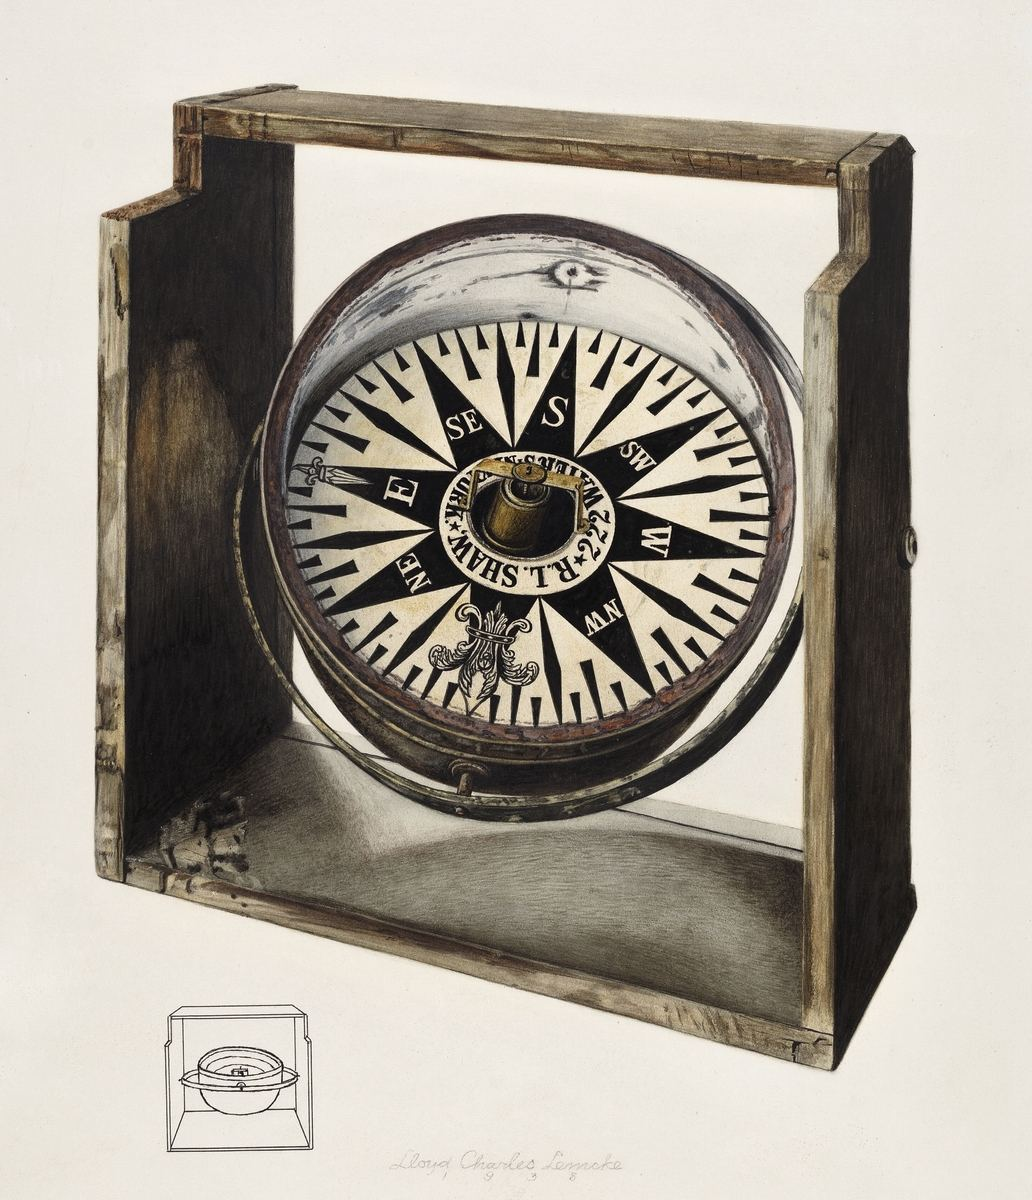
\includegraphics[width=1\linewidth]{imagenes/geo}

Hasta hace poco tiempo, labores como la producción de mapas y el análisis espacial estaban reservadas para especialistas. La complejidad de las tareas y al alto costo de producción y adquisición de datos geográficos funcionaban como barrera difícil de superar. Pero durante las dos últimas décadas la tecnología digital cambió el panorama. Una brusca caída en el costo asociado a adquirir y procesar información geográfica (pensemos en satélites y computadoras multiplicándose y bajando de precio) dio paso al mapa digital como herramienta universal. El consumo de sofisticados mapas y otros productos geográficos se volvió masivo y cotidiano, con \emph{Google Maps} como el exponente más conocido. Apenas había pasado la novedad de disponer de mapas en alta resolución de todo el mundo accesibles al instante desde nuestros escritorios, cuando la llegada de los \emph{smartphones} popularizó el acceso en cualquier momento y lugar.

El mismo proceso que nos convirtió a todos en consumidores constantes de información geográfica también nos da la oportunidad de ser los productores. Sin dudas, hacer mapas se ha vuelto más fácil que nunca antes. Existen cada vez más repositorios con información georreferenciada de acceso publico, datasets que incluyen información precisa sobre la ubicación geográfica de sus registros. Al mismo tiempo, maduran y se hacen más fáciles de usar las herramientas para análisis y visualización espacial.

En los procesos sociales, el ``dónde'' suele ser un aspecto clave. Es central para quienes estudiamos -por ejemplo- las ciudades o las dinámicas de la política, siempre tan arraigadas a lo territorial. Esto vuelve al mapa una de las herramientas de visualización más importantes que podemos emplear.

Del mismo modo, también crece la disponibilidad datos que incluyen fecha y hora. Para entender datasets con datos en gran volumen que poseen atributos de posición y tiempo, es útil visualizar el ritmo en el que ocurren (diario, mensual, anual, etc) tanto como la forma en la que se distribuyen en el espacio.

\hypertarget{trabajando-con-fechas}{%
\section{Trabajando con fechas}\label{trabajando-con-fechas}}

Continuemos aprovechando el dataset con delitos registrados durante el 2020 en Buenos Aires, ahora para practicar el manejo de fechas y horas.

Esta vez usaremos una versión aún más completa, que incluye columnas con la fecha completa, la hora, y la ubicación de cada incidente:

\begin{Shaded}
\begin{Highlighting}[]
\NormalTok{delitos }\OtherTok{\textless{}{-}} \FunctionTok{read.csv}\NormalTok{(}\StringTok{"https://cdaj.netlify.app/data/delitos\_fecha\_lugar.csv"}\NormalTok{)}
\end{Highlighting}
\end{Shaded}

Las primeras filas del dataset lucen así (:

\begin{verbatim}
##    anio    fecha franja                  tipo         subtipo     uso_armas
## 1  2020 01/01/20     10 Hurto (sin violencia)                              
## 2  2020 01/01/20     22             Homicidio       Femicidio              
## 3  2020 01/01/20     19  Robo (con violencia)                              
## 4  2020 01/01/20     17  Robo (con violencia)                              
## 5  2020 01/01/20      2 Hurto (sin violencia)                              
## 6  2020 01/01/20      5  Robo (con violencia)                              
## 7  2020 01/01/20      2 Hurto (sin violencia)                              
## 8  2020 01/01/20      2  Robo (con violencia)                              
## 9  2020 01/01/20      1 Hurto (sin violencia)                              
## 10 2020 01/01/20      8 Hurto (sin violencia)                              
## 11 2020 01/01/20     23              Lesiones  Siniestro Vial              
## 12 2020 01/01/20      6 Hurto (sin violencia)                              
## 13 2020 01/01/20     14  Robo (con violencia)                              
## 14 2020 01/01/20      3  Robo (con violencia)                              
## 15 2020 01/01/20      6  Robo (con violencia)                 Arma cortante
## 16 2020 01/01/20     10              Lesiones  Siniestro Vial              
## 17 2020 01/01/20      2  Robo (con violencia) Con uso de moto              
## 18 2020 01/01/20      9 Hurto (sin violencia) Hurto Automotor              
## 19 2020 01/01/20      4 Hurto (sin violencia)                              
## 20 2020 01/01/20      2  Robo (con violencia)                 Arma de fuego
## 21 2020 01/01/20      7  Robo (con violencia)                              
## 22 2020 01/01/20      4              Lesiones  Siniestro Vial              
## 23 2020 01/01/20     20  Robo (con violencia)                              
## 24 2020 01/01/20      3  Robo (con violencia)                              
## 25 2020 01/01/20      7  Robo (con violencia)                              
## 26 2020 01/01/20      6  Robo (con violencia)                              
## 27 2020 01/01/20     10  Robo (con violencia)                 Arma cortante
## 28 2020 01/01/20     17 Hurto (sin violencia)                              
## 29 2020 01/01/20      6  Robo (con violencia) Con uso de moto              
## 30 2020 01/01/20     10              Lesiones  Siniestro Vial              
## 31 2020 01/01/20     13 Hurto (sin violencia)                              
## 32 2020 01/01/20     16 Hurto (sin violencia)                              
## 33 2020 01/01/20     13 Hurto (sin violencia)                              
## 34 2020 01/01/20      1 Hurto (sin violencia)                              
## 35 2020 01/01/20      9 Hurto (sin violencia)                              
## 36 2020 01/01/20     20  Robo (con violencia)                              
## 37 2020 01/01/20     18  Robo (con violencia)                              
## 38 2020 01/01/20     13  Robo (con violencia)                              
## 39 2020 01/01/20     20  Robo (con violencia)                              
## 40 2020 01/01/20      6  Robo (con violencia)                              
## 41 2020 01/01/20     13 Hurto (sin violencia)                              
## 42 2020 01/01/20     12 Hurto (sin violencia)                              
## 43 2020 01/01/20      1 Hurto (sin violencia)                              
## 44 2020 01/01/20      0  Robo (con violencia)                              
## 45 2020 01/01/20     11  Robo (con violencia)                              
## 46 2020 01/01/20     18  Robo (con violencia)                              
## 47 2020 01/01/20     13 Hurto (sin violencia)                              
## 48 2020 01/01/20     18 Hurto (sin violencia)                              
## 49 2020 01/01/20      3  Robo (con violencia)                              
## 50 2020 01/01/20     21  Robo (con violencia)                 Arma de fuego
##               barrio comuna   latitud  longitud victimas
## 1          Versalles     10 -34.62664 -58.52761       NA
## 2       Villa Devoto     11 -34.61127 -58.52539        1
## 3          Versalles     10 -34.62543 -58.52501       NA
## 4          Versalles     10 -34.62543 -58.52501       NA
## 5       Villa Devoto     11 -34.60679 -58.52073       NA
## 6          Mataderos      9 -34.65520 -58.51430       NA
## 7         Villa Luro     10 -34.62763 -58.51336       NA
## 8       Monte Castro     10 -34.62131 -58.51289       NA
## 9          Mataderos      9 -34.65903 -58.51064       NA
## 10      Villa Devoto     11 -34.58959 -58.50954       NA
## 11      Villa Devoto     11 -34.60425 -58.50919       NA
## 12      Villa Devoto     11 -34.59979 -58.50919       NA
## 13         Mataderos      9 -34.65414 -58.50910       NA
## 14         Mataderos      9 -34.65417 -58.50762       NA
## 15         Mataderos      9 -34.65504 -58.50650       NA
## 16     Villa Urquiza     12 -34.56947 -58.50527       NA
## 17      Monte Castro     10 -34.61168 -58.50441       NA
## 18        Villa Luro     10 -34.63923 -58.50340       NA
## 19   Vélez Sársfield     10 -34.62402 -58.50248       NA
## 20         Mataderos      9 -34.66381 -58.50178       NA
## 21         Mataderos      9 -34.67398 -58.50164       NA
## 22          Saavedra     12 -34.55205 -58.50065       NA
## 23         Mataderos      9 -34.67192 -58.50007       NA
## 24         Agronomía     15 -34.59368 -58.49854       NA
## 25      Villa Lugano      8 -34.67673 -58.49640       NA
## 26  Villa Del Parque     11 -34.60146 -58.49416       NA
## 27      Villa Lugano      8 -34.67129 -58.49055       NA
## 28 Parque Avellaneda      9 -34.64712 -58.48987       NA
## 29      Villa Lugano      8 -34.67787 -58.48783       NA
## 30          Floresta     10 -34.62562 -58.48725       NA
## 31      Villa Lugano      8 -34.67148 -58.48589       NA
## 32          Saavedra     12 -34.55026 -58.48576       NA
## 33     Villa Urquiza     12 -34.57234 -58.48483       NA
## 34  Villa Del Parque     11 -34.60116 -58.48417       NA
## 35 Parque Avellaneda      9 -34.64202 -58.48325       NA
## 36     Villa Urquiza     12 -34.57197 -58.48277       NA
## 37     Villa Urquiza     12 -34.57197 -58.48277       NA
## 38      Villa Lugano      8 -34.67083 -58.48170       NA
## 39          Floresta     10 -34.63207 -58.48097       NA
## 40          Saavedra     12 -34.55291 -58.48000       NA
## 41     Villa Urquiza     12 -34.56588 -58.47953       NA
## 42          Saavedra     12 -34.54437 -58.47945       NA
## 43  Villa Del Parque     11 -34.60497 -58.47889       NA
## 44  Villa Santa Rita     11 -34.62153 -58.47872       NA
## 45  Villa Santa Rita     11 -34.62153 -58.47872       NA
## 46          Saavedra     12 -34.54178 -58.47792       NA
## 47 Parque Avellaneda      9 -34.65569 -58.47779       NA
## 48  Villa Santa Rita     11 -34.61864 -58.47745       NA
## 49 Parque Avellaneda      9 -34.65925 -58.47704       NA
## 50          Floresta     10 -34.63076 -58.47638       NA
\end{verbatim}

Teniendo en cuenta que el dataset es del 2020, el Primer Año de la Pandemia COVID, nos podríamos preguntar si se ve algún descenso brusco en robos, hurtos, homicidios o siniestros viales con el inicio de la cuarentena. Para responder eso, vamos a tener que lidiar con datos de tipo ``fecha''. Esto podría ser bastante engorroso, pero por suerte podemos usar una herramienta que simplifica las cosas.

\hypertarget{la-fecha-como-clase-de-variable}{%
\subsection{La fecha como clase de variable}\label{la-fecha-como-clase-de-variable}}

La fecha es un tipo de dato que puede ser expresado de muchas maneras, dependiendo de que nos interese tener en cuenta: el día de la semana al que corresponde, el mes, el año, etc. El paquete \href{https://lubridate.tidyverse.org/}{\texttt{lubridate}} hace fácil tomar una variable que contiene fechas en cualquier formato (por ejemplo ``20/07/2020'') para extraer el atributo relacionado que deseemos (como su día, ``lunes'', o su mes, ``julio''). Cuando instalamos \texttt{tidyverse} recibimos también \texttt{lubridate} -es parte del ``pack''-, así que ya deberíamos tenerlo listo para usar.

Para empezar, convertimos el campo ``fecha'' al tipo de dato especializado, que se llama\ldots{} fecha (\emph{date}). Aquí tenemos que prestar atención al formato en que aparecen los datos de la columna, en general algo como ``30-07-2018'' (día, mes, año) o ``30-07-2018 12:14:24'' (día, mes, año y hora, minutos, segundos). Con nuestros datos se da el primer caso, por lo cual la función para convertir ese campo en fecha es \texttt{dmy()}; para el segundo caso, seria \texttt{dmy\_hms()}.

\begin{Shaded}
\begin{Highlighting}[]
\FunctionTok{library}\NormalTok{(lubridate)}

\NormalTok{delitos}\SpecialCharTok{$}\NormalTok{fecha }\OtherTok{\textless{}{-}} \FunctionTok{dmy}\NormalTok{(delitos}\SpecialCharTok{$}\NormalTok{fecha)}
\end{Highlighting}
\end{Shaded}

\texttt{lubridate} usa un formato memotécnico para nombrar sus funciones de conversión de texto a fecha.
Para saber que función utilizar según el formato en que aparecen las fechas, es cuestión de determinar en que orden aparecen año, mes y día (y horas y minutos si estuvieran).

Por ejemplo, un campo que registran fechas en formato similar a ``4/26/17'' o a ``4-26-2017'' implica ``mes - día - año'' y por tanto en ambos casos puede convertirse a fecha con \texttt{mdy()} (la ``y'' es por \emph{year}).

Repasemos algunas de los nuevos trucos que podemos hacer con el tiempo. Tomemos cinco fechas elegidas al azar:

\begin{Shaded}
\begin{Highlighting}[]
\NormalTok{muestra\_de\_fechas }\OtherTok{\textless{}{-}} \FunctionTok{sample}\NormalTok{(delitos}\SpecialCharTok{$}\NormalTok{fecha, }\DecValTok{5}\NormalTok{)}

\NormalTok{muestra\_de\_fechas}
\end{Highlighting}
\end{Shaded}

\begin{verbatim}
## [1] "2020-12-07" "2020-11-05" "2020-09-21" "2020-09-27" "2020-02-21"
\end{verbatim}

Mediante las funciones disponibles en \texttt{lubridate}, podemos extraer:

\begin{itemize}
\tightlist
\item
  El día de la semana al que corresponde cada fecha:
\end{itemize}

\begin{Shaded}
\begin{Highlighting}[]
\FunctionTok{wday}\NormalTok{(muestra\_de\_fechas)}
\end{Highlighting}
\end{Shaded}

\begin{verbatim}
## [1] 2 5 2 1 6
\end{verbatim}

\begin{Shaded}
\begin{Highlighting}[]
\FunctionTok{wday}\NormalTok{(muestra\_de\_fechas, }\AttributeTok{label =} \ConstantTok{TRUE}\NormalTok{)}
\end{Highlighting}
\end{Shaded}

\begin{verbatim}
## [1] lun jue lun dom vie
## Levels: dom < lun < mar < mié < jue < vie < sáb
\end{verbatim}

\begin{itemize}
\tightlist
\item
  El mes:
\end{itemize}

\begin{Shaded}
\begin{Highlighting}[]
\FunctionTok{month}\NormalTok{(muestra\_de\_fechas)}
\end{Highlighting}
\end{Shaded}

\begin{verbatim}
## [1] 12 11  9  9  2
\end{verbatim}

\begin{Shaded}
\begin{Highlighting}[]
\FunctionTok{month}\NormalTok{(muestra\_de\_fechas, }\AttributeTok{label =} \ConstantTok{TRUE}\NormalTok{)}
\end{Highlighting}
\end{Shaded}

\begin{verbatim}
## [1] dic nov sep sep feb
## 12 Levels: ene < feb < mar < abr < may < jun < jul < ago < sep < ... < dic
\end{verbatim}

\begin{itemize}
\tightlist
\item
  El año:
\end{itemize}

\begin{Shaded}
\begin{Highlighting}[]
\FunctionTok{year}\NormalTok{(muestra\_de\_fechas)}
\end{Highlighting}
\end{Shaded}

\begin{verbatim}
## [1] 2020 2020 2020 2020 2020
\end{verbatim}

Y varias opciones más, que se pueden repasar en \url{https://cran.r-project.org/web/packages/lubridate/vignettes/lubridate.html}

Con lo visto hasta aquí, tenemos suficiente para mostrar patrones temporales en los datos.

Empecemos por un gráfico de barras (\texttt{geom\_bar()}) con la cantidad de eventos registrados por mes. Para que aparezca un conteo por mes del año, asignaremos al eje de las \(x\) el \emph{mes} al que corresponde cada valor de la columna ``fecha'', o sea \texttt{month(fecha,\ label\ =\ TRUE)}:

\begin{Shaded}
\begin{Highlighting}[]
\FunctionTok{library}\NormalTok{(tidyverse) }\CommentTok{\# cargamos la librería en caso de no haberlo hecho antes}
\end{Highlighting}
\end{Shaded}

\begin{Shaded}
\begin{Highlighting}[]
\FunctionTok{ggplot}\NormalTok{(delitos) }\SpecialCharTok{+} 
    \FunctionTok{geom\_bar}\NormalTok{(}\FunctionTok{aes}\NormalTok{(}\AttributeTok{x =} \FunctionTok{month}\NormalTok{(fecha, }\AttributeTok{label =} \ConstantTok{TRUE}\NormalTok{)))}
\end{Highlighting}
\end{Shaded}

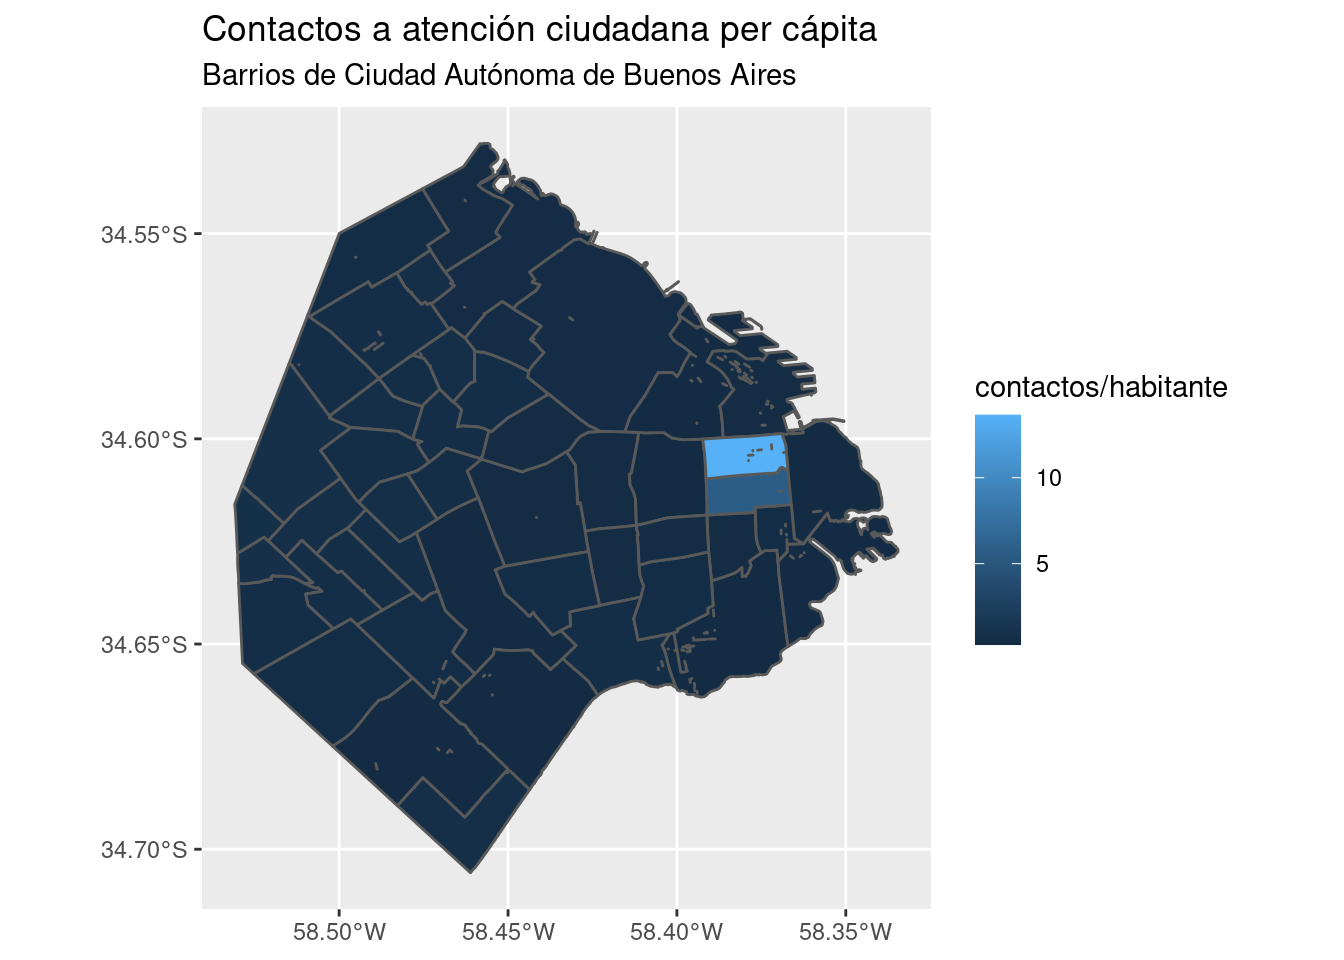
\includegraphics{CD_AJ_files/figure-latex/unnamed-chunk-142-1.pdf}

(Hemos usado el parámetro \texttt{label\ =\ TRUE} para obtener el nombre del mes en lugar de su número, o sea ``dic'' en lugar de ``12''. Prueben realizar el gráfico sin ese parámetro en la llamada a \texttt{month()} para ver que pasa.)

En el gráfico, se ve una reducción drástica a partir de la cuarentena decretada en abril. Y también un incremento gradual y sostenido a partir de allí, que de todos modos no llega a los niveles pre-pandemia de enero y febrero.

Para ver la composición interna de los conteos mensuales, cuantos casos corresponden a cada categoría, podemos hacer un gráfico de ``barras apiladas'' como vimos en la clase 3. La sintaxis es igual que antes, pero esta vez asignamos la variable \emph{tipo}''\_ al color de relleno de las barras determinado por el parámetro \texttt{fill}.

\begin{Shaded}
\begin{Highlighting}[]
\FunctionTok{ggplot}\NormalTok{(delitos) }\SpecialCharTok{+} 
    \FunctionTok{geom\_bar}\NormalTok{(}\FunctionTok{aes}\NormalTok{(}\AttributeTok{x =} \FunctionTok{month}\NormalTok{(fecha, }\AttributeTok{label =} \ConstantTok{TRUE}\NormalTok{), }\AttributeTok{fill =}\NormalTok{ tipo))}
\end{Highlighting}
\end{Shaded}

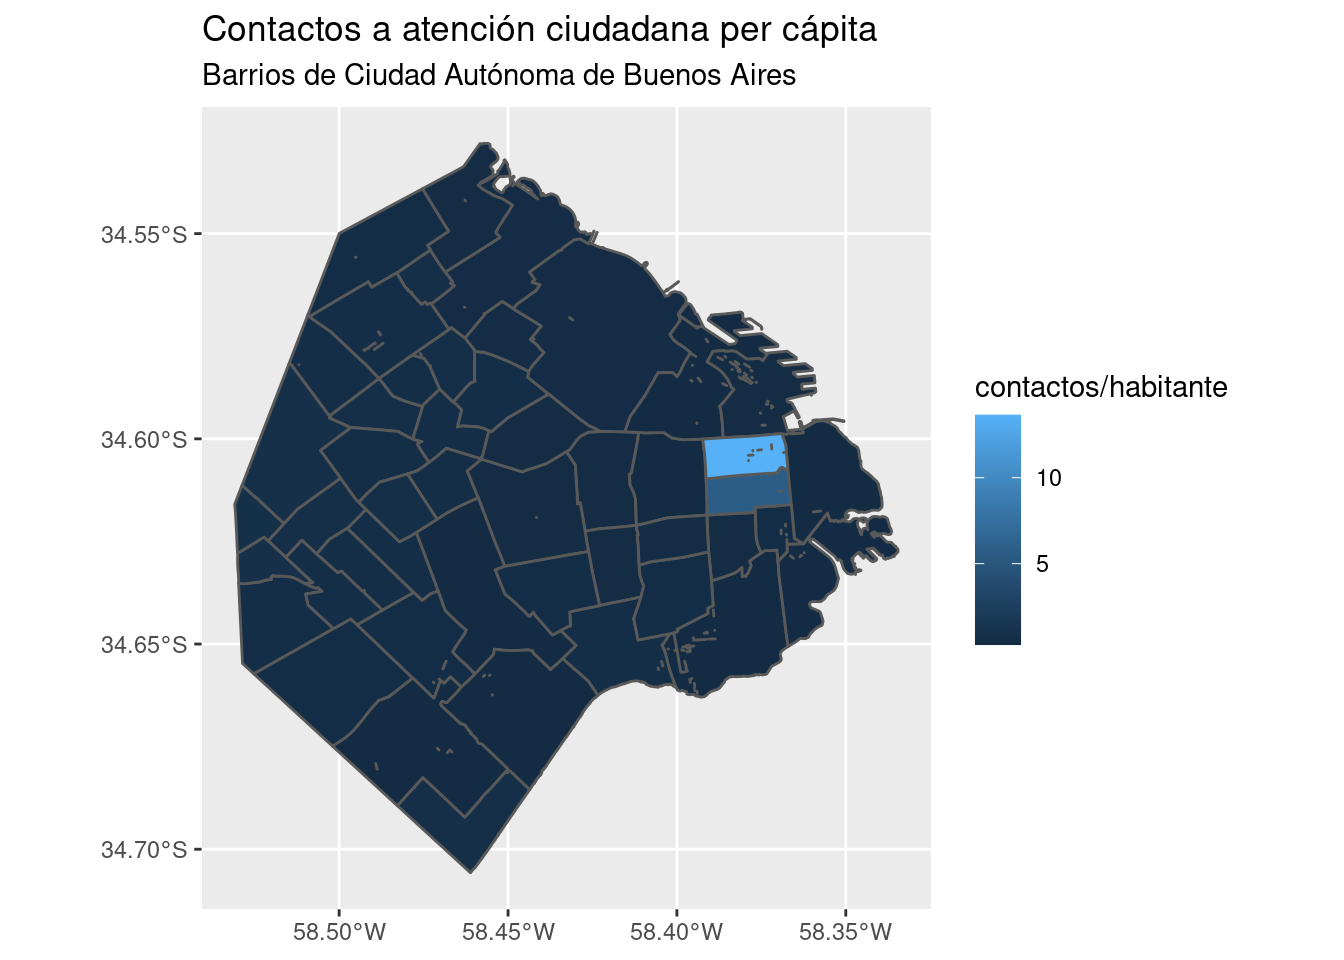
\includegraphics{CD_AJ_files/figure-latex/unnamed-chunk-143-1.pdf}

Las barras apiladas son prolijas, pero pueden hacer difícil evaluar la evolución de categorías individuales. Recordemos que para mostrar los subconjuntos en barras independientes, una al lado de la otra, podemos usar el parámetro \texttt{position\ =\ "dodge"}. Inténtenlo agregando el parámetro al ejercicio anterior para ver como queda.

Ahora comparemos la cantidad de eventos registrados, por tipo, para cada día de la semana. Basta con usar la función que extrae el día de la semana, \texttt{wday()}, en lugar de \texttt{month()}. Lo demás es idéntico, incluyendo el uso de \texttt{label\ =\ TRUE} para que obtener el nombre del día -``lun''-, en lugar de su posición en la semana -``2'', porque para \texttt{lubridate} las semanas empiezan el domingo-.

\begin{Shaded}
\begin{Highlighting}[]
\FunctionTok{ggplot}\NormalTok{(delitos) }\SpecialCharTok{+} 
    \FunctionTok{geom\_bar}\NormalTok{(}\FunctionTok{aes}\NormalTok{(}\AttributeTok{x =} \FunctionTok{wday}\NormalTok{(fecha, }\AttributeTok{label =} \ConstantTok{TRUE}\NormalTok{), }\AttributeTok{fill =}\NormalTok{ tipo))}
\end{Highlighting}
\end{Shaded}

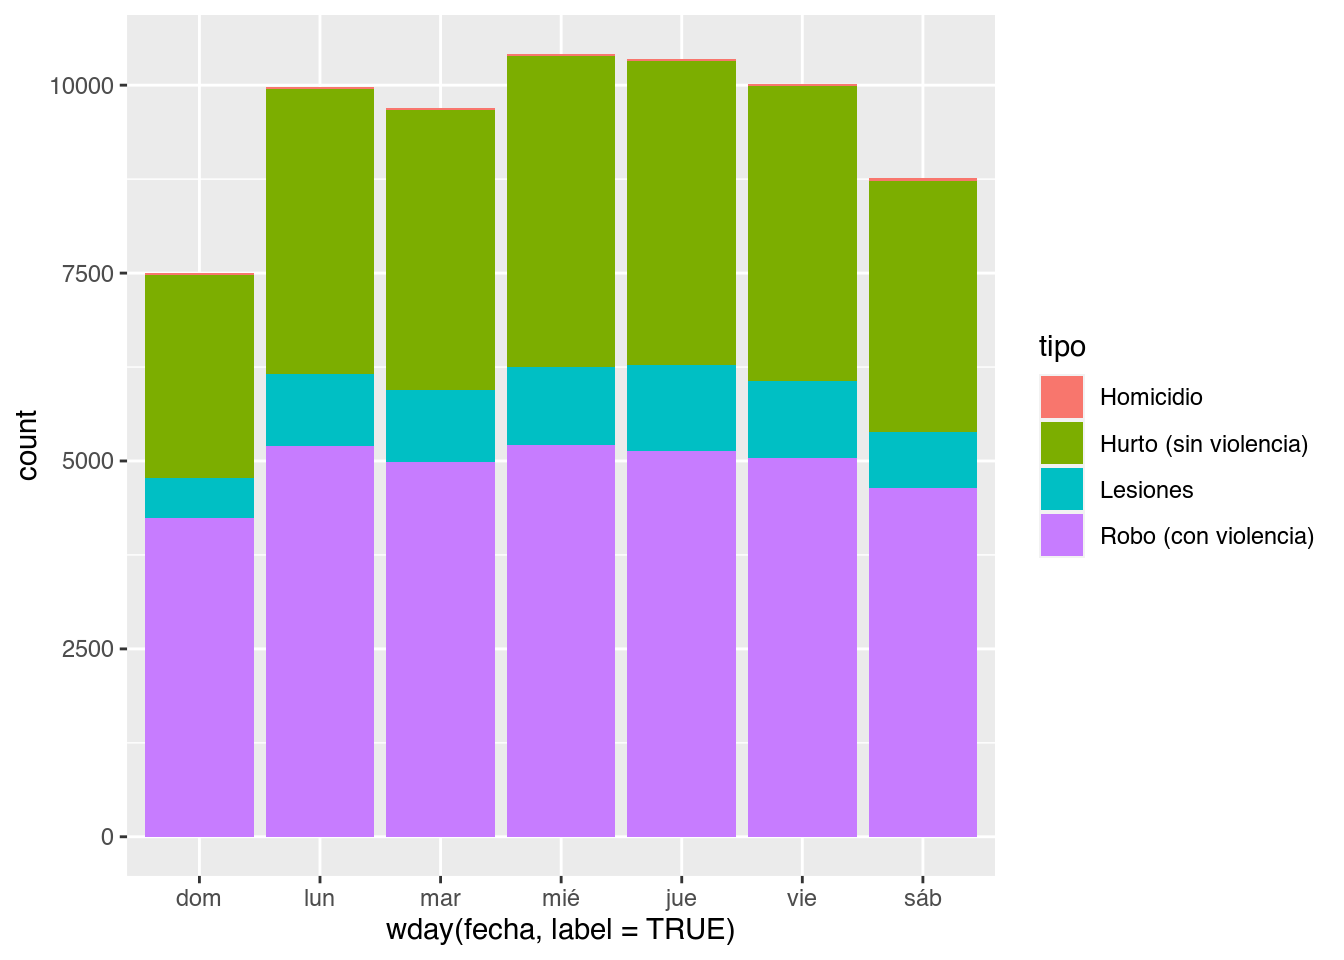
\includegraphics{CD_AJ_files/figure-latex/unnamed-chunk-144-1.pdf}

Como era de esperar, durante los fines de semana se observa una menor cantidad de eventos, aunque quizás no en la categoría Homicidio, que es difícil de discernir por su relativa escasez. Para solucionar el problema podríamos filtrar los datos antes de visualizarlos, como hemos hecho antes con la función \texttt{filter()}, mostrando sólo la categoría de interés.

Otra opción, que probaremos ahora, es una visualización en ``facetas''. Se trata de generar una visualización que muestra distintos aspectos de los datos en paneles separados. Con un ejemplo vamos a dejarlo mas claro. Para realizar un gráfico en facetas, basta con sumar una línea con la función \texttt{facet\_wrap(vars(x,\ y,\ ...))}, dónde ``x'', ``y'', etc son los nombres de las variables cuyas categorías recibirán paneles distintos. Intentémoslo con el último gráfico, agregando ``tipo'' como variable a facetar:

\begin{Shaded}
\begin{Highlighting}[]
\FunctionTok{ggplot}\NormalTok{(delitos) }\SpecialCharTok{+} 
    \FunctionTok{geom\_bar}\NormalTok{(}\FunctionTok{aes}\NormalTok{(}\AttributeTok{x =} \FunctionTok{wday}\NormalTok{(fecha, }\AttributeTok{label =} \ConstantTok{TRUE}\NormalTok{), }\AttributeTok{fill =}\NormalTok{ tipo)) }\SpecialCharTok{+}
    \FunctionTok{facet\_wrap}\NormalTok{(}\FunctionTok{vars}\NormalTok{(tipo))}
\end{Highlighting}
\end{Shaded}

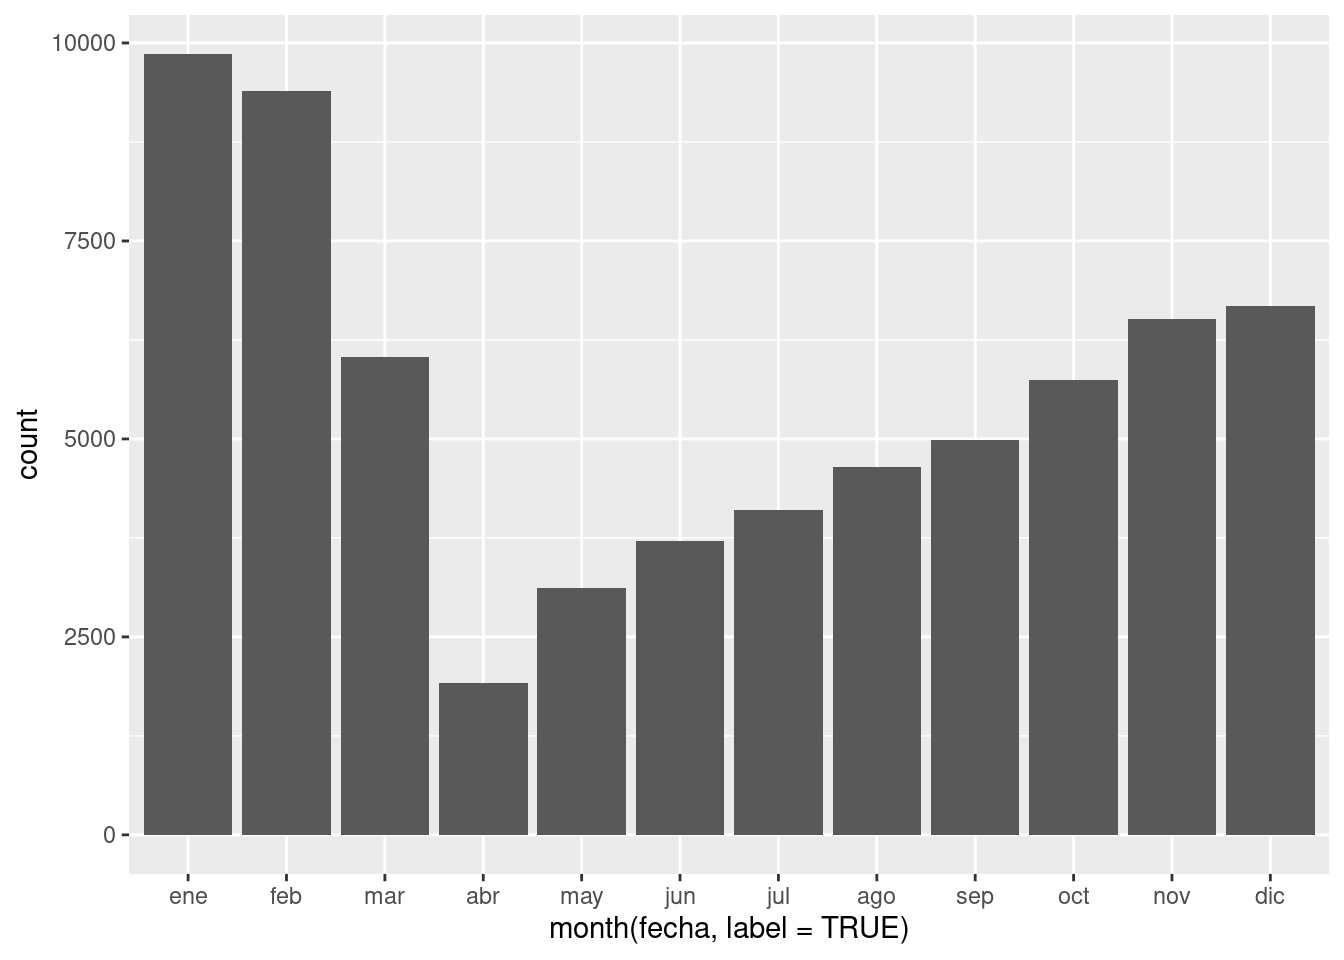
\includegraphics{CD_AJ_files/figure-latex/unnamed-chunk-145-1.pdf}

Obtuvimos barras separadas, pero los homicidios siguen difíciles de distinguir. Se debe a que por defecto \texttt{facet\_wrap()} mantiene a escala todos los paneles, de manera que se puedan comparar cantidades de forma directa. La desventaja es que se pierde legibilidad de categorías con valores ínfimos en comparación con otras. Por eso disponemos del parámetro \texttt{scales}, que permite graficar los datos con escala libre, vía \texttt{scales\ =\ "free"}. Probemos:

\begin{Shaded}
\begin{Highlighting}[]
\FunctionTok{ggplot}\NormalTok{(delitos) }\SpecialCharTok{+} 
    \FunctionTok{geom\_bar}\NormalTok{(}\FunctionTok{aes}\NormalTok{(}\AttributeTok{x =} \FunctionTok{wday}\NormalTok{(fecha, }\AttributeTok{label =} \ConstantTok{TRUE}\NormalTok{), }\AttributeTok{fill =}\NormalTok{ tipo)) }\SpecialCharTok{+}
    \FunctionTok{facet\_wrap}\NormalTok{(}\FunctionTok{vars}\NormalTok{(tipo), }\AttributeTok{scales =} \StringTok{"free"}\NormalTok{)}
\end{Highlighting}
\end{Shaded}

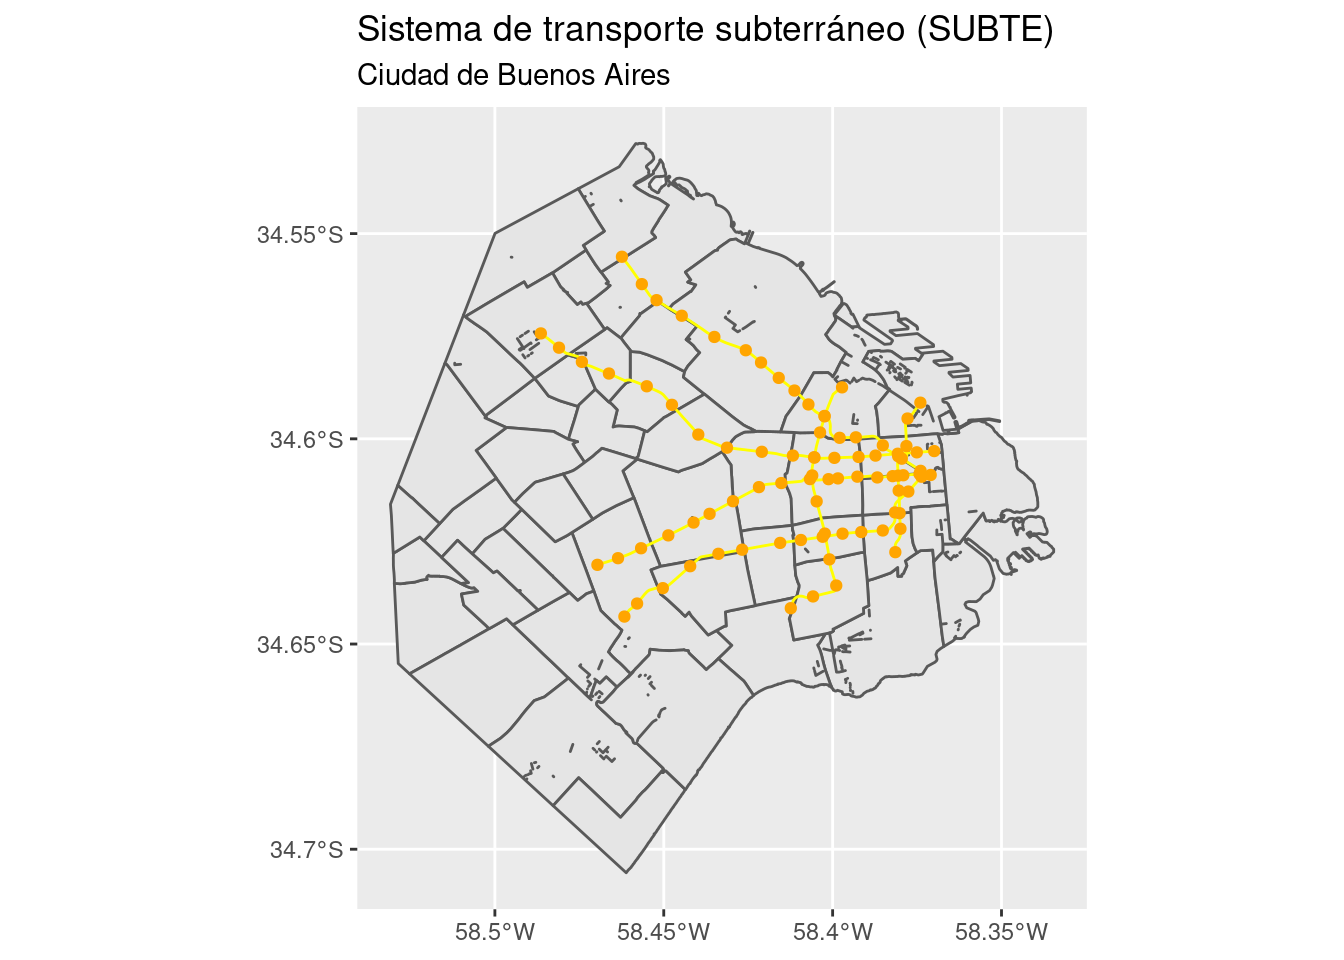
\includegraphics{CD_AJ_files/figure-latex/unnamed-chunk-146-1.pdf}
Ahora queda más claro que los homicidios siguen un patrón diario distinto al de las demás categorías. También que, en términos relativos, las lesiones son las que mas se reducen durante los fines de semana.

También podemos evaluar el ritmo según la hora del día. ¿Cómo se haría con nuestro dataset?

\hypertarget{mirando-al-espacio}{%
\section{Mirando al espacio}\label{mirando-al-espacio}}

Pasemos ahora al análisis espacial de nuestros datos. Nuestro dataset incluye columnas de \emph{longitud} y \emph{latitud} para cada registro, lo cual identifica su posición sobre la superficie de la Tierra\ldots{} ¡y nos permite realizar mapas!. Para ello usaremos el paquete \texttt{ggmap}, que aporta funciones para hacer visualizaciones de tipo mapa usando las técnicas de ggplot que ya hemos practicado.

Representar en forma precisa una posición geográfica es un todo un reto cuando necesitamos mostrar rasgos de una superficie tridimensional cuasi-esférica (¡la Tierra!) en superficies planas (papel o pantallas). La solución toma la forma de sistemas de coordenadas de referencia (CRS por sus siglas en inglés), y de proyecciones cartográficas.

Los CRS son un sistema de números que definen ubicaciones sobre la superficie de la Tierra; funcionan como direcciones usando latitud y longitud para definir posiciones en los ejes norte-sur y este-oeste. Hay muchos, muchos tipos de CRS, y en general hace falta saber con cuál trabajamos. Sin embargo, existe una especie de regla no escrita: si nuestros datos georreferenciados no aclaran cuál es su sistema de coordenadas, podemos asumir que usan el llamado WGS84 o ``Mercator''. Eso mismo presupone \texttt{ggmap}, y como nuestro dataset efectivamente usa coordenadas WGS84, todos los ejercicios que siguen saldrán bien aún sin especificar el CRS.

Como siempre, si es la primera vez que vamos a usar el paquete tenemos que instalarlo:

\begin{Shaded}
\begin{Highlighting}[]
\FunctionTok{install.packages}\NormalTok{(}\StringTok{"ggmap"}\NormalTok{)}
\end{Highlighting}
\end{Shaded}

Y con eso resuelto ya podremos activarlo cuando lo necesitemos:

\begin{Shaded}
\begin{Highlighting}[]
\FunctionTok{library}\NormalTok{(ggmap)}
\end{Highlighting}
\end{Shaded}

\hypertarget{obteniendo-un-mapa-base}{%
\subsection{Obteniendo un mapa base}\label{obteniendo-un-mapa-base}}

Para dar contexto que guíe a la audiencia es útil proyectar nuestra información georreferenciada sobre un mapa de fondo que muestre la posición de caminos, nombres de localidades, accidentes geográficos y otros hitos. Estos mapas usados como lienzo sobre el cual mostrar datos espaciales son conocidos como ``mapas base'', o \emph{basemaps}. Guardar por nuestra cuenta información cartográfica con alto nivel de detalle de cualquier lugar del mundo es impracticable, pero por suerte existen servicios en internet que lo hacen por nosotros como \href{http://maps.stamen.com}{Stamen Maps}, ¡que es de uso gratuito!.

\begin{center}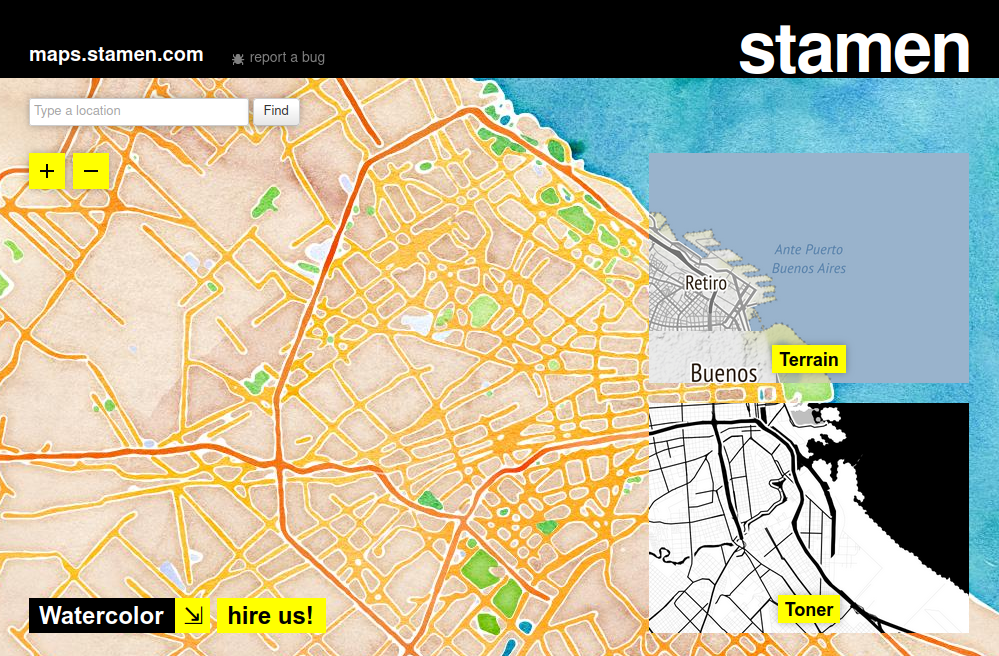
\includegraphics[width=0.85\linewidth]{imagenes/stamen} \end{center}

\emph{El sitio web de Stamen Maps}

Para incluir mapas base en nuestras visualizaciones podemos usar las funciones del paquete \href{https://github.com/dkahle/ggmap}{\texttt{ggmap}}, que complementa a ggplot agregando funciones que permiten adquirir y visualizar mapas en forma fácil.

Lo activamos:

\begin{Shaded}
\begin{Highlighting}[]
\FunctionTok{library}\NormalTok{(ggmap)}
\end{Highlighting}
\end{Shaded}

Ahora, para obtener un mapa base del área donde se encuentran los datos que queremos mostrar, necesitamos determinar su ``bounding box'': el rango de latitud y longitud que forma un rectángulo conteniendo todas sus posiciones. En resumidas cuentas, se trata de los valores de latitud máxima y mínima, y de longitud máxima y mínima, de nuestros datos georreferenciados.

Los proveedores de mapas online suelen solicitar los valores en este orden: izquierda, abajo, derecha, arriba. Es decir, posición mas al oeste, posición mas al sur, posición mas al este, posición mas al norte.
Cuando disponemos de un dataframe georreferenciado, obtener la \emph{bounding box} de su contenido es bastante fácil usando \texttt{st\_bbox}, una función del paquete \texttt{sf} que recupera esas cuatro coordenadas clave. Por ejemplo \texttt{st\_bbox(radios)} obtiene las coordenadas del rectángulo de territorio que abarca los radios censales de Buenos Aires. Luego de guardar las coordenadas en una variable, les ponemos los nombres que permitirán que \texttt{ggmap} las identifique:

Para obtener un mapa de fondo o ``mapa base'' necesitamos obtener una \emph{bounding box} de nuestros datos: el rango de latitud y longitud que forma un rectángulo conteniendo todas sus posiciones. En resumidas cuentas, se trata de los valores de latitud máxima y mínima, y de longitud máxima y mínima, de nuestros datos georreferenciados.
No es algo que deba preocuparnos demasiado, porque podemos obtener esta información con una simple función incluida en \texttt{ggmap}:

\begin{Shaded}
\begin{Highlighting}[]
\NormalTok{bbox }\OtherTok{\textless{}{-}} \FunctionTok{make\_bbox}\NormalTok{(delitos}\SpecialCharTok{$}\NormalTok{longitud, delitos}\SpecialCharTok{$}\NormalTok{latitud)}

\NormalTok{bbox}
\end{Highlighting}
\end{Shaded}

\begin{verbatim}
##      left    bottom     right       top 
## -58.54046 -34.71247 -58.33403 -34.52172
\end{verbatim}

En base a la ``bounding box'' solicitamos nuestro mapa base:

\begin{Shaded}
\begin{Highlighting}[]
\NormalTok{CABA }\OtherTok{\textless{}{-}} \FunctionTok{get\_stamenmap}\NormalTok{(}\AttributeTok{bbox =}\NormalTok{ bbox, }\AttributeTok{maptype =} \StringTok{"toner"}\NormalTok{, }\AttributeTok{zoom =} \DecValTok{12}\NormalTok{)}
\end{Highlighting}
\end{Shaded}

Para verlo:

\begin{Shaded}
\begin{Highlighting}[]
\FunctionTok{ggmap}\NormalTok{(CABA)}
\end{Highlighting}
\end{Shaded}

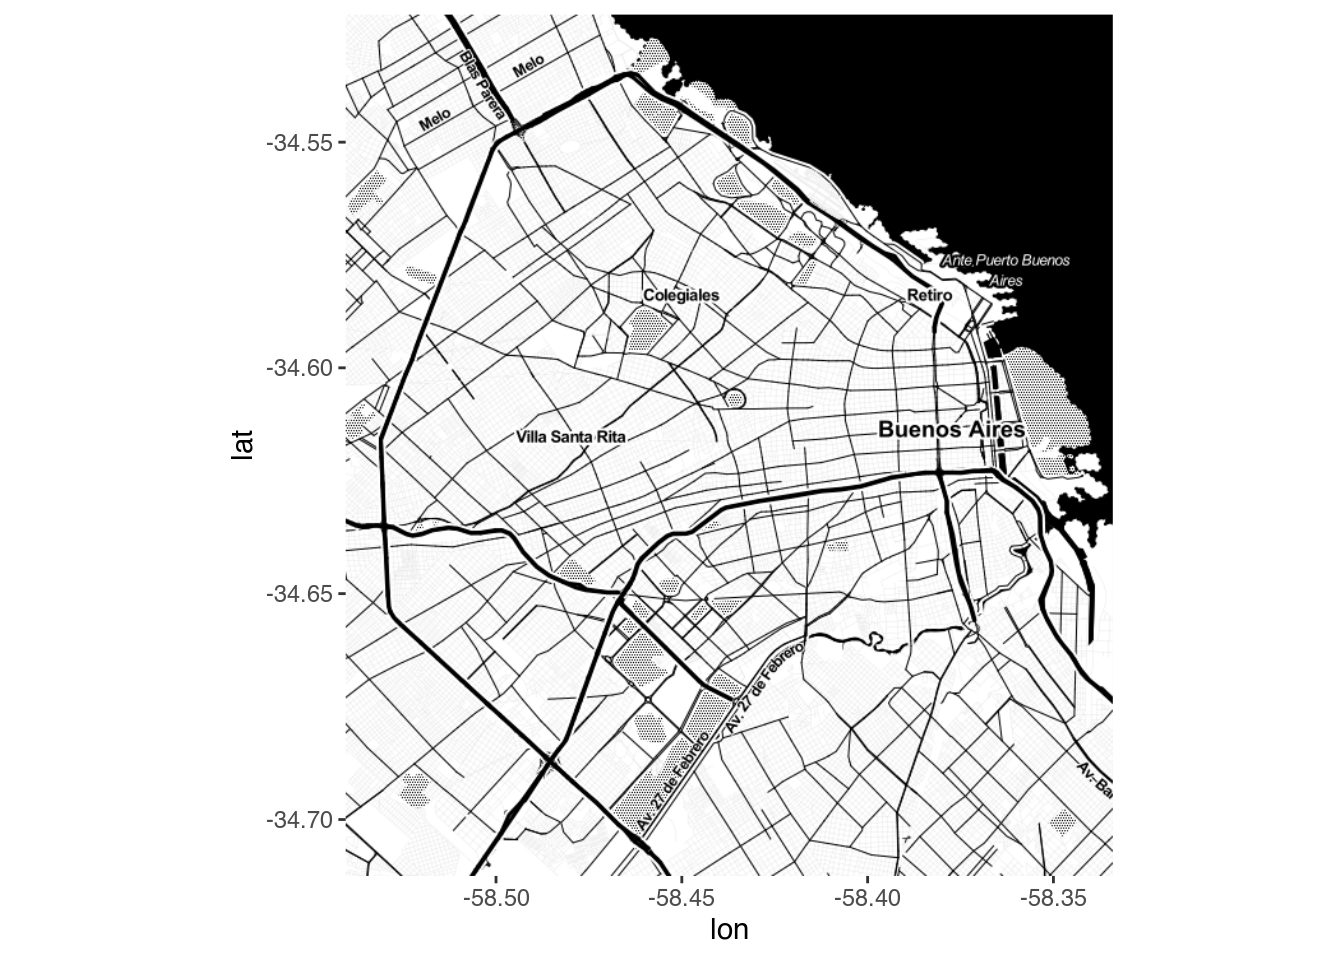
\includegraphics{CD_AJ_files/figure-latex/unnamed-chunk-153-1.pdf}

Stamen ofrece varios estilos de mapa base, que pueden revisarse en su \href{http://maps.stamen.com}{sitio web}.
Entre ellos:

\begin{itemize}
\tightlist
\item
  \texttt{terrain} (usado por defecto)
\item
  \texttt{toner} (monocromático, buena opción para visualizar datos proyectados por encima)
\item
  \texttt{toner-lite} (versión alternativa de toner, con menos contraste visual)
\item
  \texttt{watercolor} (hay que probarlo para apreciarlo, pero digamos que es artístico)
\end{itemize}

Se adquieren usando el parámetro \emph{maptype}.
Por ejemplo, \texttt{get\_stamenmap(bbox\ =\ bbox,\ maptype\ =\ "watercolor",\ zoom\ =\ 12)}

\hypertarget{de-coordenadas-al-mapa}{%
\subsection{De coordenadas al mapa}\label{de-coordenadas-al-mapa}}

De aquí en más podemos suporponer nuestros datos en distintas capas sobre el mapa, con la misma sintaxis que conocemos de ggplot. Para mapear las ubicaciones de los delitos en el dataset, usamos \texttt{geom\_point()} y los campos de longitud y latitud para los ejes \(x\) e \(y\):

En ocasiones los datos de longitud y latitud son leídos como texto (tipo ``chr''), en lugar de números. Si eso ocurre el mapeo no va a funcionar, porque necesita datos numéricos para latitud y longitud. Para solucionarlo, podemos intentar convertir las columnas de coordenadas a tipo numérico. Algo así como \texttt{misdatos\$longitud\ \textless{}-\ as.numeric(misdatos\$longitud)}

\begin{Shaded}
\begin{Highlighting}[]
\FunctionTok{ggmap}\NormalTok{(CABA) }\SpecialCharTok{+}
    \FunctionTok{geom\_point}\NormalTok{(}\AttributeTok{data =}\NormalTok{ delitos, }\FunctionTok{aes}\NormalTok{(}\AttributeTok{x =}\NormalTok{ longitud, }\AttributeTok{y =}\NormalTok{ latitud))}
\end{Highlighting}
\end{Shaded}

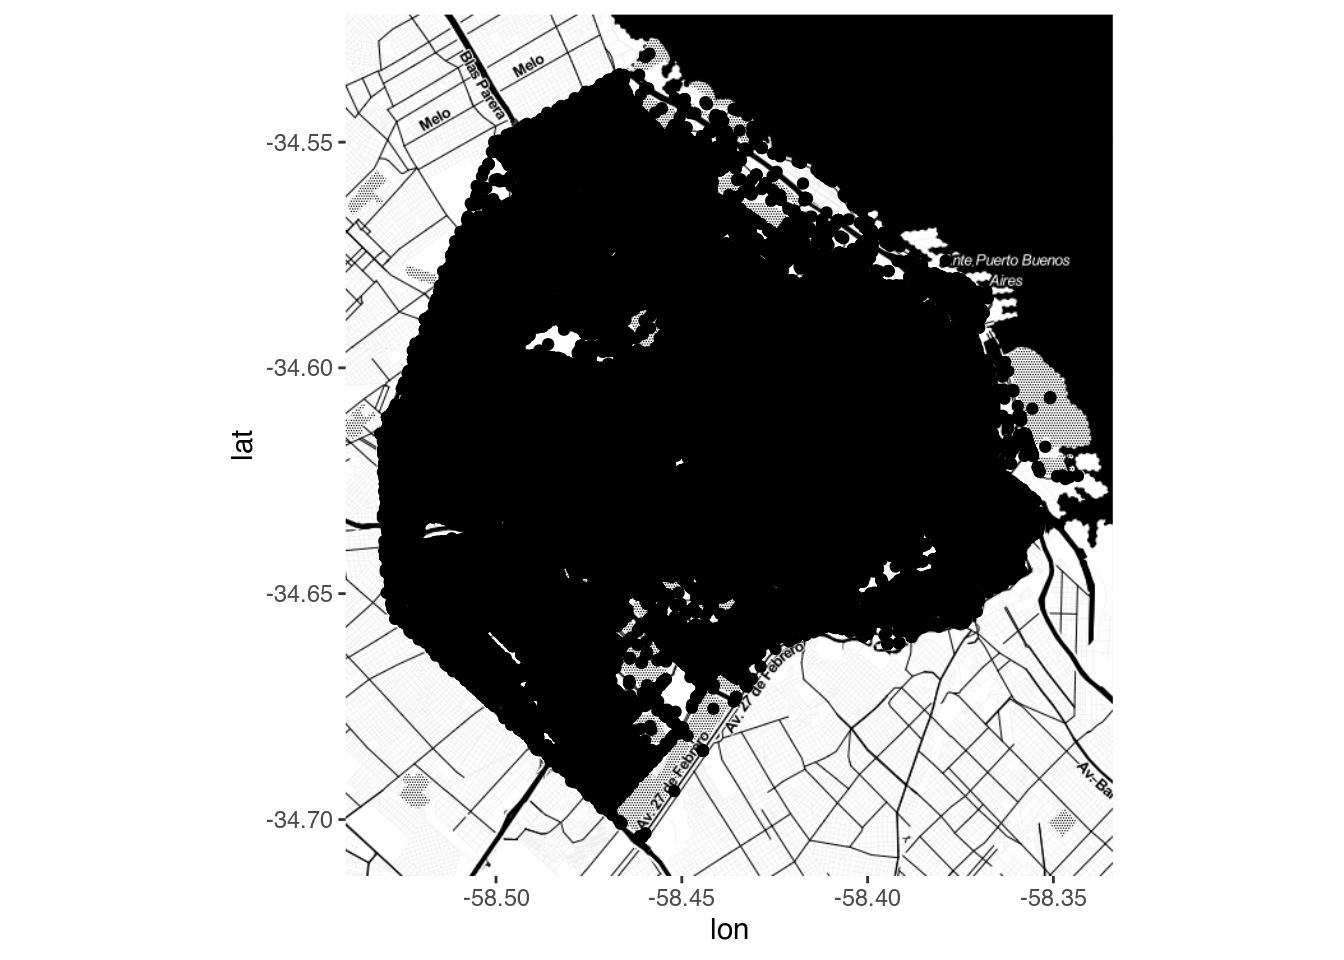
\includegraphics{CD_AJ_files/figure-latex/unnamed-chunk-154-1.pdf}

Aquí nos topamos con un problema habitual al trabajar con grandes volúmenes de datos. Hay tantos puntos proyectados sobre el mapa, que se hace imposible interpretar dónde existen más o menos. Hacemos algunos ajustes:

\begin{itemize}
\tightlist
\item
  un color que resalte más contra el mapa base, y que no se confunda con él
\item
  un tamaño de punto más pequeño
\item
  y aplicación de una ligera transparencia
\end{itemize}

Todo ello vía los atributos ``color'', ``size'' y ``alpha''. ¿Cuál es el valor ideal para cada uno? En general, hay que recurrir a la prueba y error para encontrar la receta justa. Probemos con \texttt{color\ =\ "orange"}, \texttt{size\ =\ 0.1} y \texttt{alpha\ =\ 0.1}:

\begin{Shaded}
\begin{Highlighting}[]
\FunctionTok{ggmap}\NormalTok{(CABA) }\SpecialCharTok{+}
    \FunctionTok{geom\_point}\NormalTok{(}\AttributeTok{data =}\NormalTok{ delitos, }\FunctionTok{aes}\NormalTok{(}\AttributeTok{x =}\NormalTok{ longitud, }\AttributeTok{y =}\NormalTok{ latitud),}
               \AttributeTok{color =} \StringTok{"orange"}\NormalTok{, }\AttributeTok{size =} \FloatTok{0.1}\NormalTok{, }\AttributeTok{alpha =} \FloatTok{0.1}\NormalTok{)}
\end{Highlighting}
\end{Shaded}

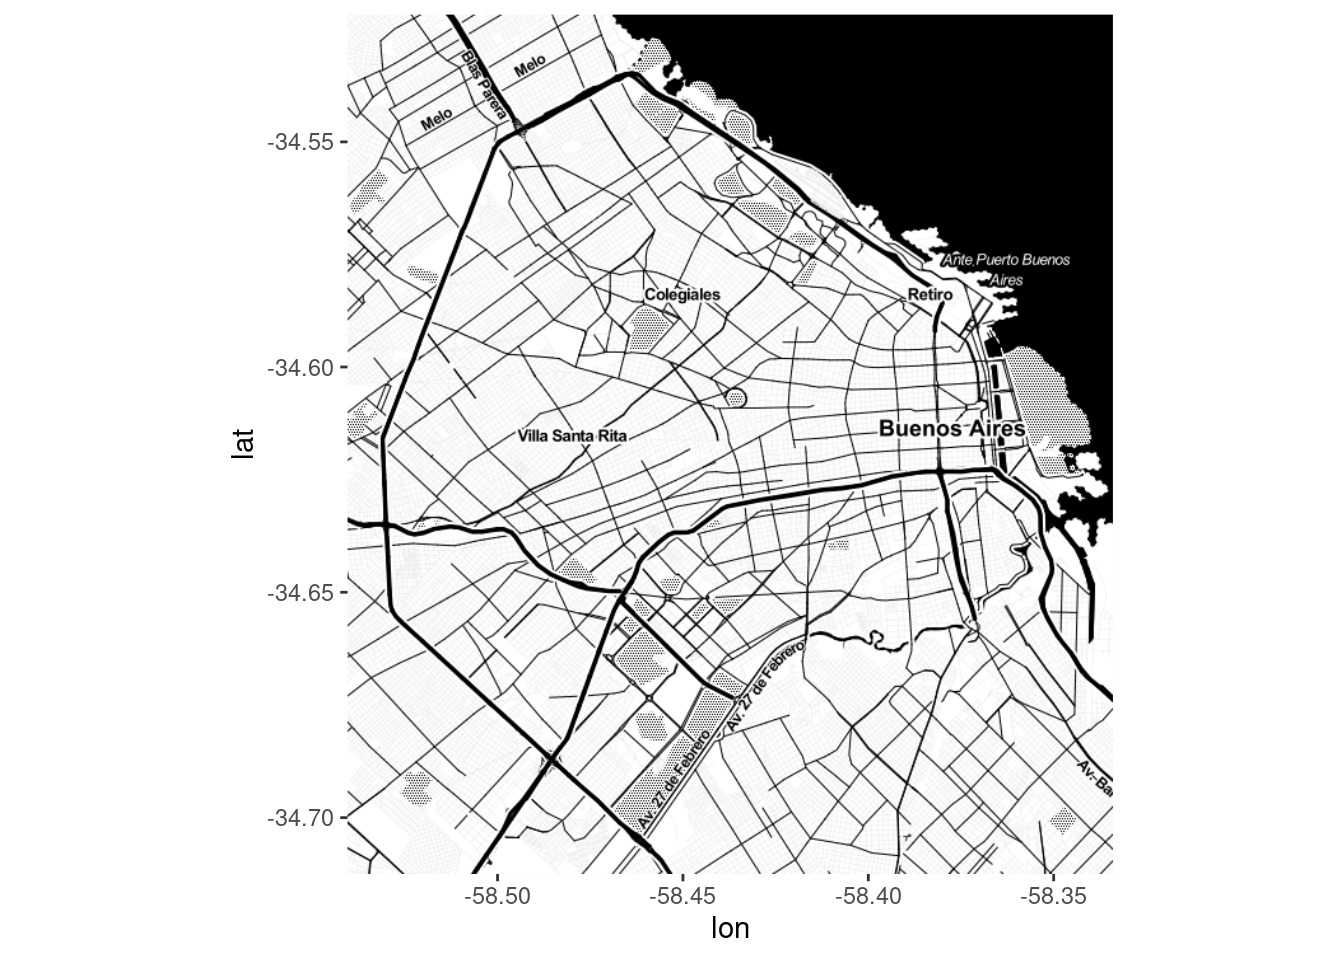
\includegraphics{CD_AJ_files/figure-latex/unnamed-chunk-155-1.pdf}

Ahora si aparecen ciertos patrones, por ejemplo la mayor frecuencia de casos de casos cerca de las principales de circulación de la ciudad. Aún así, se hace difícil identificar de un golpe de vista las ``zonas calientes'', las áreas de máxima concentración.

\hypertarget{mapas-de-densidad}{%
\subsection{Mapas de densidad}\label{mapas-de-densidad}}

Una solución práctica para el problema de la cantidad de puntos es una técnica llamada ``binning'': dividir el espacio en una grilla de celdas, contar cuantos puntos caen dentro de cada una, y visualizar las cantidades agregadas. En el mundo \texttt{ggplot} esto se lleva a cabo con \texttt{geom\_bind2d()}.

\begin{Shaded}
\begin{Highlighting}[]
\FunctionTok{ggmap}\NormalTok{(CABA) }\SpecialCharTok{+}
    \FunctionTok{geom\_bin2d}\NormalTok{(}\AttributeTok{data =}\NormalTok{ delitos, }\FunctionTok{aes}\NormalTok{(}\AttributeTok{x =}\NormalTok{ longitud, }\AttributeTok{y =}\NormalTok{ latitud))}
\end{Highlighting}
\end{Shaded}

\includegraphics{CD_AJ_files/figure-latex/unnamed-chunk-156-1.pdf}

Ahora si, resaltan las áreas de mayor concentración de incidentes. Se puede mejorar un poco el gráfico usando:

\begin{itemize}
\tightlist
\item
  una mayor cantidad de celdas para aumentar la resolución
\item
  una escala de colores diseñada para ayudar a detectar diferencias por tonalidad, como Viridis.
\end{itemize}

la cantidad de celdas se define con el parámetro ``bins'', por ejemplo \texttt{bins\ =\ 100}. La escala de color Viridis, como ya habíamos visto, se agrega sumando una llamada a \texttt{scale\_fill\_viridis\_c()} -porque aquí la data es continua, si fuera discreta usaríamos \texttt{scale\_fill\_viridis\_d()}.

\begin{Shaded}
\begin{Highlighting}[]
\FunctionTok{ggmap}\NormalTok{(CABA) }\SpecialCharTok{+}
    \FunctionTok{geom\_bin2d}\NormalTok{(}\AttributeTok{data =}\NormalTok{ delitos, }\FunctionTok{aes}\NormalTok{(}\AttributeTok{x =}\NormalTok{ longitud, }\AttributeTok{y =}\NormalTok{ latitud), }\AttributeTok{bins =} \DecValTok{100}\NormalTok{) }\SpecialCharTok{+}
    \FunctionTok{scale\_fill\_viridis\_c}\NormalTok{()}
\end{Highlighting}
\end{Shaded}

\includegraphics{CD_AJ_files/figure-latex/unnamed-chunk-157-1.pdf}

Una alternativa al \emph{binning} es la llamada \emph{kernel density estimation}, muy utilizada en aplicaciones de análisis espacial para estimar la intensidad de una determinada variable en cualquier punto del área analizada, incluso en aquellos para los cuales no hay observaciones. La idea es asumir que los valores observados corresponden a una distribución continua sobre el espacio, y determinar cual es la más probable en base a los puntos donde existen datos. Podemos visualizar esta distribución estimada \texttt{geom\_density2d\_filled} así:

\begin{Shaded}
\begin{Highlighting}[]
\FunctionTok{ggmap}\NormalTok{(CABA) }\SpecialCharTok{+}
    \FunctionTok{geom\_density2d\_filled}\NormalTok{(}\AttributeTok{data =}\NormalTok{ delitos, }\FunctionTok{aes}\NormalTok{(}\AttributeTok{x =}\NormalTok{ longitud, }\AttributeTok{y =}\NormalTok{ latitud), }\AttributeTok{alpha =} \FloatTok{0.5}\NormalTok{) }
\end{Highlighting}
\end{Shaded}

\includegraphics{CD_AJ_files/figure-latex/unnamed-chunk-158-1.pdf}
Nótese que aplicamos transparencia usando el parámetro \texttt{alpha\ =\ 0.5}. ¿Por qué? ¿Qué pasa si lo quitamos?

\hypertarget{visualizando-multiples-categoruxedas}{%
\subsection{Visualizando multiples categorías}\label{visualizando-multiples-categoruxedas}}

Hasta aquí hemos analizado la distribución espacial de eventos en su totalidad, sin diferenciar su tipo. Veamos ahora las diferencias por categoría. Podemos reintentar el mapa de puntos, esta vez diferenciándolos por color. Recuperamos el código que usamos antes para mostrar puntos, y esta vez asignamos la columna ``tipo'' al atributo estético \texttt{color}:

\begin{Shaded}
\begin{Highlighting}[]
\FunctionTok{ggmap}\NormalTok{(CABA) }\SpecialCharTok{+}
    \FunctionTok{geom\_point}\NormalTok{(}\AttributeTok{data =}\NormalTok{ delitos, }
               \FunctionTok{aes}\NormalTok{(}\AttributeTok{x =}\NormalTok{ longitud, }\AttributeTok{y =}\NormalTok{ latitud, }\AttributeTok{color =}\NormalTok{ tipo),}
               \AttributeTok{size =} \FloatTok{0.1}\NormalTok{, }\AttributeTok{alpha =} \FloatTok{0.1}\NormalTok{)}
\end{Highlighting}
\end{Shaded}

\includegraphics{CD_AJ_files/figure-latex/unnamed-chunk-159-1.pdf}

Aquí tenemos dos problemas:

\begin{itemize}
\item
  La leyenda (``tipo\_delito'') es difícil de leer, dado que muestra los puntos tal como los definimos: pequeños y con mucha transparencia. Esos atributos son útiles en el mapa, donde tenemos cientos de miles de puntos, pero muy poco prácticos para la leyenda, donde sólo hay un minúsculo punto por etiqueta.
\item
  Los puntos sobre el mapa se superponen en tal medida que es difícil identificar patrones espaciales distintos según su categoría.
\end{itemize}

El primer problema se resuelve fijando ``a mano'' los atributos de la leyenda, asi:

\begin{Shaded}
\begin{Highlighting}[]
\FunctionTok{ggmap}\NormalTok{(CABA) }\SpecialCharTok{+}
    \FunctionTok{geom\_point}\NormalTok{(}\AttributeTok{data =}\NormalTok{ delitos,}
               \FunctionTok{aes}\NormalTok{(}\AttributeTok{x =}\NormalTok{ longitud, }\AttributeTok{y =}\NormalTok{ latitud, }\AttributeTok{color =}\NormalTok{ tipo),}
               \AttributeTok{size =} \FloatTok{0.1}\NormalTok{, }\AttributeTok{alpha =} \FloatTok{0.1}\NormalTok{) }\SpecialCharTok{+}
    \FunctionTok{guides}\NormalTok{(}\AttributeTok{color =} \FunctionTok{guide\_legend}\NormalTok{(}\AttributeTok{override.aes =} \FunctionTok{list}\NormalTok{(}\AttributeTok{size =} \DecValTok{1}\NormalTok{, }\AttributeTok{alpha =} \DecValTok{1}\NormalTok{)))}
\end{Highlighting}
\end{Shaded}

\includegraphics{CD_AJ_files/figure-latex/unnamed-chunk-160-1.pdf}

El segundo, usando facetado para mostrar en su propio mapa a cada categoría:

\begin{Shaded}
\begin{Highlighting}[]
\FunctionTok{ggmap}\NormalTok{(CABA) }\SpecialCharTok{+}
    \FunctionTok{geom\_point}\NormalTok{(}\AttributeTok{data =}\NormalTok{ delitos,}
               \FunctionTok{aes}\NormalTok{(}\AttributeTok{x =}\NormalTok{ longitud, }\AttributeTok{y =}\NormalTok{ latitud, }\AttributeTok{color =}\NormalTok{ tipo),}
               \AttributeTok{size =} \FloatTok{0.1}\NormalTok{, }\AttributeTok{alpha =} \FloatTok{0.1}\NormalTok{) }\SpecialCharTok{+}
    \FunctionTok{guides}\NormalTok{(}\AttributeTok{color =} \FunctionTok{guide\_legend}\NormalTok{(}\AttributeTok{override.aes =} \FunctionTok{list}\NormalTok{(}\AttributeTok{size =} \DecValTok{1}\NormalTok{, }\AttributeTok{alpha =} \DecValTok{1}\NormalTok{))) }\SpecialCharTok{+}
    \FunctionTok{facet\_wrap}\NormalTok{(}\FunctionTok{vars}\NormalTok{(tipo))}
\end{Highlighting}
\end{Shaded}

\includegraphics{CD_AJ_files/figure-latex/unnamed-chunk-161-1.pdf}

El facetado ayuda a que no se nos mezclen los colores, y hace evidente cuales categorías son mas frecuentes que otras. Pero con nuestra abundancia de puntos no ayuda encontrar los sitios de alta concentración, y hace que se pierdan de vista los casos de la categoría poco frecuente (homicidios).

Para hacer las diferencias aún mas nítidas, podemos facetar una estimación de densidad en lugar de puntos. ¿Cómo lo haríamos?

\begin{Shaded}
\begin{Highlighting}[]
\FunctionTok{ggmap}\NormalTok{(CABA) }\SpecialCharTok{+}
    \FunctionTok{geom\_density2d\_filled}\NormalTok{(}\AttributeTok{data =}\NormalTok{ delitos, }\FunctionTok{aes}\NormalTok{(}\AttributeTok{x =}\NormalTok{ longitud, }\AttributeTok{y =}\NormalTok{ latitud), }\AttributeTok{alpha =} \FloatTok{0.5}\NormalTok{) }\SpecialCharTok{+}
    \FunctionTok{facet\_wrap}\NormalTok{(}\FunctionTok{vars}\NormalTok{(tipo))}
\end{Highlighting}
\end{Shaded}

\includegraphics{CD_AJ_files/figure-latex/unnamed-chunk-162-1.pdf}

\hypertarget{combinando-espacio-y-tiempo}{%
\section{Combinando espacio y tiempo}\label{combinando-espacio-y-tiempo}}

El facetado también nos permite visualizar el cambio de posición a través del tiempo.

Por ejemplo, podemos comparar cierto tipo delito (hurto sin violencia) mostrando dónde ocurre en cada día de la semana.

Y luego mostramos sólo las filas del dataframe donde la columna tipo contiene ``Homicidio'',
- en forma de puntos en el mapa (\texttt{geom\_point()}),
- con el ``subtipo'' de homicidio representado por el \texttt{color} de los puntos
- y un facetado por día de la semana (\texttt{facet\_wrap(vars(wday(fecha,\ label\ =\ TRUE)))})

\begin{Shaded}
\begin{Highlighting}[]
\FunctionTok{ggmap}\NormalTok{(CABA) }\SpecialCharTok{+}
    \FunctionTok{geom\_point}\NormalTok{(}\AttributeTok{data =} \FunctionTok{filter}\NormalTok{(delitos, tipo }\SpecialCharTok{==} \StringTok{"Homicidio"}\NormalTok{),}
               \FunctionTok{aes}\NormalTok{(}\AttributeTok{x =}\NormalTok{ longitud, }\AttributeTok{y =}\NormalTok{ latitud, }\AttributeTok{color =}\NormalTok{ subtipo), }\AttributeTok{alpha =}\NormalTok{ .}\DecValTok{5}\NormalTok{) }\SpecialCharTok{+}
    \FunctionTok{facet\_wrap}\NormalTok{(}\FunctionTok{vars}\NormalTok{(}\FunctionTok{wday}\NormalTok{(fecha, }\AttributeTok{label =} \ConstantTok{TRUE}\NormalTok{)))}
\end{Highlighting}
\end{Shaded}

\includegraphics{CD_AJ_files/figure-latex/unnamed-chunk-163-1.pdf}

Vale aclarar que el poco elegante \texttt{facet\_wrap(vars(wday(fecha,\ label\ =\ TRUE)))} podría cambiarse por un más legible \texttt{facet\_wrap(vars(dia\_semana))} si como paso previo agregamos al dataframe la columna ``dia\_semana'', guardando allí el valor obtenido con \texttt{wday()}.

Volviendo al tiempo y el espacio, también podemos concentrarnos en un tipo de delito en particular, y evaluar en que zonas se concentra de acuerdo a la hora del día. Nuestra data ya tiene la hora del día declarada en una columna, ``franja''. Si no fuera así, y tuviéramos la hora como parte de la fecha (estilo ``2020-09-18 14:00:00'') podríamos obtenerla con ayuda de \texttt{hour()} que funciona de forma similar a las ya vistas \texttt{month()} y \texttt{wday()}.

Entonces, mostremos sólo las filas del dataframe donde la columna tipo contiene ``Hurto (sin violencia)'',
- en forma de mapa de densidad (\texttt{geom\_density2d\_filled()}),
- y un facetado por hora del día (\texttt{facet\_wrap(vars(franja))})

\begin{Shaded}
\begin{Highlighting}[]
\FunctionTok{ggmap}\NormalTok{(CABA) }\SpecialCharTok{+}
    \FunctionTok{geom\_density2d\_filled}\NormalTok{(}\AttributeTok{data =} \FunctionTok{filter}\NormalTok{(delitos, tipo }\SpecialCharTok{==} \StringTok{"Hurto (sin violencia)"}\NormalTok{),}
               \FunctionTok{aes}\NormalTok{(}\AttributeTok{x =}\NormalTok{ longitud, }\AttributeTok{y =}\NormalTok{ latitud), }\AttributeTok{alpha =}\NormalTok{ .}\DecValTok{5}\NormalTok{) }\SpecialCharTok{+}
    \FunctionTok{facet\_wrap}\NormalTok{(}\FunctionTok{vars}\NormalTok{(franja))}
\end{Highlighting}
\end{Shaded}

\includegraphics{CD_AJ_files/figure-latex/unnamed-chunk-164-1.pdf}

En el resultado se puede ver como los hurtos se concentran nítidamente en las áreas de mayor actividad comercial durante el día (lo que los porteños llaman ``el centro''), sobre todo desde el mediodía hasta 4 o 5 de la tarde, cuando pierde intensidad y se dispersa en la dirección de las principales avenidas de la ciudad.

Para terminar, pulimos la visualización
- filtrando las filas que registran la franja horaria como desconocida (\texttt{!is.na(franja)})
- retirando la leyenda, ya que nos interesa mostrar como se mueve la densidad a lo largo del día más que las cantidades
- eligiendo la cantidad de filas en la que se distribuirán las facetas (\texttt{nrow\ =\ 4})
- agregando título, subtítulo, y nota al pie con fuente
- eligiendo un tema apropiado

\begin{Shaded}
\begin{Highlighting}[]
\FunctionTok{ggmap}\NormalTok{(CABA) }\SpecialCharTok{+}
    \FunctionTok{geom\_density2d\_filled}\NormalTok{(}\AttributeTok{data =} \FunctionTok{filter}\NormalTok{(delitos, }\SpecialCharTok{!}\FunctionTok{is.na}\NormalTok{(franja), tipo }\SpecialCharTok{==} \StringTok{"Hurto (sin violencia)"}\NormalTok{),}
               \FunctionTok{aes}\NormalTok{(}\AttributeTok{x =}\NormalTok{ longitud, }\AttributeTok{y =}\NormalTok{ latitud), }\AttributeTok{alpha =}\NormalTok{ .}\DecValTok{5}\NormalTok{) }\SpecialCharTok{+}
    \FunctionTok{guides}\NormalTok{(}\AttributeTok{fill =} \ConstantTok{FALSE}\NormalTok{) }\SpecialCharTok{+}
    \FunctionTok{facet\_wrap}\NormalTok{(}\FunctionTok{vars}\NormalTok{(franja), }\AttributeTok{nrow =} \DecValTok{4}\NormalTok{) }\SpecialCharTok{+}
    \FunctionTok{labs}\NormalTok{(}\AttributeTok{title =} \StringTok{"Ciudad de Buenos Aires: concentración espacial de hurtos"}\NormalTok{,}
         \AttributeTok{subtitle =} \StringTok{"según hora del día, durante el año 2020"}\NormalTok{,}
         \AttributeTok{caption =} \StringTok{"fuente: https://mapa.seguridadciudad.gob.ar"}\NormalTok{) }\SpecialCharTok{+}
    \FunctionTok{theme\_void}\NormalTok{()}
\end{Highlighting}
\end{Shaded}

\includegraphics{CD_AJ_files/figure-latex/unnamed-chunk-165-1.pdf}

\hypertarget{ejercicios-4}{%
\section{Ejercicios}\label{ejercicios-4}}

I. Utilizando la información disponible en el dataset de delitos, creemos un gráfico un gráfico de líneas con \texttt{geom\_line()} que muestre el ritmo horario para cada tipo. ¿Qué patrones se vislumbran? ¿Qué franja horaria representan la ``hora pico'' (u ``hora punta'') para cada categoría?

\begin{enumerate}
\def\labelenumi{\Roman{enumi}.}
\setcounter{enumi}{1}
\tightlist
\item
  Volvamos al mapa de puntos que realizamos en la seción 5.1.2, donde ajustamos los atributos ``color'', ``size'' y ``alpha'' para mejorar los resultados, además de probar con facetados y mapas de densidad. ¿Qué otras técnicas podemos usar para lidiar con el exceso de información volcada en pantalla? Sugerencia: intentar con \texttt{geom\_count()}, que se emplea de forma similar a\texttt{geom\_point()} (véase \url{https://ggplot2.tidyverse.org/reference/geom_count.html})
\end{enumerate}

\hypertarget{modelado-estaduxedstico}{%
\chapter{Modelado estadístico}\label{modelado-estaduxedstico}}

\includegraphics[width=1\linewidth]{imagenes/modelado}

Llegamos a un tema de gran interés para quienes realizan investigaciones formales. La posición central que tiene el modelado en la investigación científica se debe a que cuantifica relaciones: permite pasar de decir ``Los afroamericanos suelen pagar más en la adquisición de autos'' a ``Los vendedores hacen ofertas finales a los afroamericanos 287 dólares más caras que a los blancos''\footnote{Véase Aires, Ian ``Venta de Autos justa. La discriminación de género y raza en las negociaciones de venta de autos'', 1991, versión en español en Ian Ayres, \emph{La discriminación en el Mercado} Univ. Palermo, Buenos Aires, 2012}. La cuantificación permite realizar comparaciones, algo clave para entender un fenómeno estudiado: antes y después, con o sin tratamiento, en un lugar o en otro.

En términos matemáticos, se habla de ``modelar'' debido a que estamos creando un modelo, una reconstrucción simplificada (¡simplificada en extremo!) de cómo funciona un proceso observado en el mundo real. En un modelo de datos, siempre tenemos al menos

\begin{itemize}
\tightlist
\item
  Una variable resultante, también llamada variable ``dependiente'',
\item
  Una o más variables predictoras, también llamadas ``explicativas''
\end{itemize}

El modelado de datos puede ser utilizado para dos propósitos:

\begin{enumerate}
\def\labelenumi{\arabic{enumi}.}
\item
  \textbf{Predecir} el valor de una variable resultante en base a valores conocidos de las variables predictoras. Aquí no interesa tanto entender cómo es que las variables interactúan entre sí, o por qué lo hacen. Mientras las predicciones sean acertadas, o se acerquen lo suficiente, el modelo cumple su cometido. Los modelos predictivos se emplean en una enorme variedad de aplicaciones: inversión en bolsa, prevención de fraude, publicidad online, fijación de primas en seguros de riesgo, etc.
\item
  \textbf{Explicar} la relación entre una variable dependiente y todas las demás (las explicativas), buscando determinar si la relación es significativa. Los modelos explicativos son los que se favorecen en investigación académica, ya que ayudan a entender el fenómeno modelado.
\end{enumerate}

Existen muchísimas técnicas para modelar datos, algunas de ellas simples como la regresión lineal, y otras mucho más complejas, como las redes neuronales. Vamos a practicar con las primeras.

La humilde regresión lineal, fácil de explicar y muy fácil de resolver con la ayuda de una computadora, es el caballito de batalla del modelado estadístico. A pesar de que no es adecuada para ciertos tipo de datos, y de que existen métodos más modernos que explotan mucho más el potencial de las computadoras, la regresión lineal sigue siendo una herramienta de uso muy extendido. Un poco por costumbre, y otro porque es el método más fácil de interpretar, lo que favorece entender y comunicar sus resultados.

Este capítulo le debe mucho a \emph{ModernDive: An Introduction to Statistical and Data Sciences via R} por Chester Ismay y Albert Y. Kim, disponible en forma gratuita en \url{http://moderndive.com/}. ModernDive es un recurso muy recomendable para quienes quieran profundizar su conocimiento más allá de los temas que veremos a continuación. Vamos a usar el paquete de R homónimo, \texttt{moderndive}, que acompaña al libro y provee funciones que facilitan el aprendizaje de modelos estadísticos.

Antes de continuar, lo instalamos (¡sólo hace falta realizar esto una vez!)

\begin{Shaded}
\begin{Highlighting}[]
\FunctionTok{install.packages}\NormalTok{(}\StringTok{"moderndive"}\NormalTok{)}
\end{Highlighting}
\end{Shaded}

Y lo activamos:

\begin{Shaded}
\begin{Highlighting}[]
\FunctionTok{library}\NormalTok{(moderndive)}
\end{Highlighting}
\end{Shaded}

\hypertarget{regresiuxf3n-lineal-simple}{%
\section{Regresión lineal simple}\label{regresiuxf3n-lineal-simple}}

La encarnación más sencilla de la regresión lineal es la simple o univariada. Tenemos nuestra variable \(y\), numérica, y una sola variable predictora \(x\), que puede ser numérica o categórica.

Para poner en práctica los conceptos repasados en este capítulo, vamos a recurrir a un dataset compilado por \href{https://fivethirtyeight.com/}{\emph{FiveThirtyEight}}, un sitio web dedicado al análisis estadístico y periodístico de datos de política, economía y deportes. Sus artículos suelen ser acompañados de los datos originales utilizados para el análisis, lo que permite a la audiencia verificar los hallazgos y realizar sus propias pesquisas.

El dataset con el que trabajaremos registra la tasa promedio de \href{https://victimconnect.org/tipos-de-delitos/crimenes-de-odio/}{crímenes de odio} reportados en Estados Unidos durante el período 2010-2015, a nivel estado, junto con indicadores demográficos de cada lugar. Los \href{https://github.com/fivethirtyeight/data/tree/master/hate-crimes}{datos} fueron presentados por \emph{FiveThirtyEight} en un \href{https://fivethirtyeight.com/features/higher-rates-of-hate-crimes-are-tied-to-income-inequality/}{artículo} que explora la relación entre desigualdad socioeconómica y crímenes de odio.

Descarguemos entonces el dataset (que hemos traducido para facilitar su uso), y echemos un vistazo como ya sabemos hacer:

\begin{Shaded}
\begin{Highlighting}[]
\NormalTok{crimenes\_odio }\OtherTok{\textless{}{-}} \FunctionTok{read.csv}\NormalTok{(}\StringTok{"https://cdaj.netlify.app/data/crimenes\_odio\_EEUU.csv"}\NormalTok{)}

\FunctionTok{summary}\NormalTok{(crimenes\_odio)}
\end{Highlighting}
\end{Shaded}

\begin{verbatim}
##     estado          mediana_ingreso_hogares pct_desocupados
##  Length:50          Min.   :35.52           Min.   :2.800  
##  Class :character   1st Qu.:48.36           1st Qu.:4.200  
##  Mode  :character   Median :54.61           Median :5.050  
##                     Mean   :54.96           Mean   :4.922  
##                     3rd Qu.:60.65           3rd Qu.:5.700  
##                     Max.   :76.17           Max.   :7.300  
##                                                            
##  pct_reside_area_metro pct_secundaria_completa pct_no_ciudadanos
##  Min.   : 31.00        Min.   :79.90           Min.   : 1.00    
##  1st Qu.: 63.00        1st Qu.:83.97           1st Qu.: 3.00    
##  Median : 78.50        Median :87.50           Median : 4.00    
##  Mean   : 74.52        Mean   :86.91           Mean   : 5.34    
##  3rd Qu.: 88.50        3rd Qu.:89.80           3rd Qu.: 8.00    
##  Max.   :100.00        Max.   :91.80           Max.   :13.00    
##                                                NA's   :3        
##  pct_pobreza_blancos  indice_gini     pct_no_blancos  pct_votantes_trump
##  Min.   : 5.00       Min.   :0.4190   Min.   : 6.00   Min.   :30.00     
##  1st Qu.: 8.00       1st Qu.:0.4400   1st Qu.:19.25   1st Qu.:42.00     
##  Median : 9.00       Median :0.4530   Median :27.50   Median :49.50     
##  Mean   : 9.28       Mean   :0.4522   Mean   :30.94   Mean   :49.90     
##  3rd Qu.:10.00       3rd Qu.:0.4657   3rd Qu.:42.00   3rd Qu.:57.75     
##  Max.   :17.00       Max.   :0.4990   Max.   :81.00   Max.   :70.00     
##                                                                         
##  crimenes_odio_100k_splc crimenes_odio_prom_100k_fbi
##  Min.   :0.06745         Min.   :0.2669             
##  1st Qu.:0.14219         1st Qu.:1.2826             
##  Median :0.22576         Median :1.9371             
##  Mean   :0.27761         Mean   :2.1924             
##  3rd Qu.:0.34681         3rd Qu.:3.1361             
##  Max.   :0.83285         Max.   :4.8019             
##  NA's   :4               NA's   :1
\end{verbatim}

Aclaremos el significado de cada columna:

\begin{longtable}[]{@{}
  >{\raggedright\arraybackslash}p{(\columnwidth - 2\tabcolsep) * \real{0.2500}}
  >{\raggedright\arraybackslash}p{(\columnwidth - 2\tabcolsep) * \real{0.7500}}@{}}
\toprule()
\begin{minipage}[b]{\linewidth}\raggedright
Variable
\end{minipage} & \begin{minipage}[b]{\linewidth}\raggedright
Definición
\end{minipage} \\
\midrule()
\endhead
\texttt{estado} & Nombre del estado \\
\texttt{mediana\_ingreso\_hogares} & Mediana del ingreso de hogares (en miles USD), 2016 \\
\texttt{pct\_desocupados} & Porcentaje de población desocupada, Sept.~2016 \\
\texttt{pct\_reside\_area\_metro} & Porcentaje de población que reside en áreas metropolitanas, 2015 \\
\texttt{pct\_secundaria\_completa} & Porcentaje de adultos (25+) con educación secundaria completa, 2009 \\
\texttt{pct\_no\_ciudadanos} & Porcentaje de población sin ciudadanía, 2015 \\
\texttt{pct\_pobreza\_blancos} & Porcentaje de residentes blancos que viven en pobreza, 2015 \\
\texttt{indice\_gini} & Indice Gini, 2015 \\
\texttt{pct\_no\_blancos} & Porcentaje de población no blanca, 2015 \\
\texttt{pct\_votantes\_trump} & Porcentaje de votantes en las elecciones presidenciales 2016 que votaron por Donald Trump \\
\texttt{crimenes\_odio\_100k\_splc} & Crímenes de odio cada 100.000 habitantes, Southern Poverty Law Center, 2016 \\
\texttt{crimenes\_odio\_prom\_100k\_fbi} & Promedio anual de crímenes de odio cada 100.000 habitante, FBI, 2010-2015 \\
\bottomrule()
\end{longtable}

Con el poder de \texttt{summary()}, comprobar que la incidencia de crímenes de odio varía de forma considerable entre estados. El promedio anual 2010-2015 reportado por el FBI (variable ``crimenes\_odio\_prom\_100k\_fbi'') va de 0,2 a casi 5 incidentes cada 100.000 habitantes. Algo similar ocurre con la cantidad reportada con otra metodología, los datos para 2016 del \emph{Southern Poverty Law Center} (``crimenes\_odio\_100k\_splc''): el rango va de apenas 0,067 incidentes cada 100.000 habitantes hasta 0,83 (¡12 veces más!).

\hypertarget{regresiuxf3n-con-una-variable-numuxe9rica}{%
\subsection{Regresión con una variable numérica}\label{regresiuxf3n-con-una-variable-numuxe9rica}}

Hagamos nuestra pregunta pregunta a contestar con una regresión lineal: ¿Cómo ha se relaciona el nivel de ingresos con la incidencia de crímenes de odio?

Como dijimos en el capítulo de visualización, los \emph{scatterplots} son útiles para mostrar la relación entre dos variables. Usemos uno para visualizar la relación entre estas dos variables, para intentar anticipar los resultados de la regresión lineal.

\begin{Shaded}
\begin{Highlighting}[]
\CommentTok{\# Si no lo hicimos antes, activamos el paquete tidyverse}
\FunctionTok{library}\NormalTok{(tidyverse)}
\end{Highlighting}
\end{Shaded}

\begin{Shaded}
\begin{Highlighting}[]
\FunctionTok{ggplot}\NormalTok{(}\AttributeTok{data =}\NormalTok{ crimenes\_odio) }\SpecialCharTok{+} 
    \FunctionTok{geom\_point}\NormalTok{(}\FunctionTok{aes}\NormalTok{(}\AttributeTok{x =}\NormalTok{ mediana\_ingreso\_hogares, }\AttributeTok{y =}\NormalTok{ crimenes\_odio\_prom\_100k\_fbi)) }\SpecialCharTok{+}
    \FunctionTok{labs}\NormalTok{(}\AttributeTok{title =} \StringTok{"Correlación entre ingesos medios por hogar y crímenes de odio"}\NormalTok{,}
         \AttributeTok{subtitle =} \StringTok{"Crímenes cada 100.000 habitantes, promedio 2010{-}2016"}\NormalTok{,}
         \AttributeTok{x =} \StringTok{"mediana de ingresos por hogar (miles USD)"}\NormalTok{,}
         \AttributeTok{y =} \StringTok{"tasa de crímenes"}\NormalTok{)}
\end{Highlighting}
\end{Shaded}

\includegraphics{CD_AJ_files/figure-latex/unnamed-chunk-171-1.pdf}

Los opiniones pueden variar pero aquí parece mostrarse una correlación más bien débil entre las variables, en forma positiva. Esto es, el incremento de la mediana de ingresos por hogar resulta en un incremento en la tasa de crímenes de odio, pero en este caso no de forma drástica. Una correlación \emph{negativa} sería lo opuesto: que el incremento de la variable explicativa estuviera asociado a un decremento de la variable explicada. Además del \emph{signo} de una correlación, otra medida importante es su intensidad. La intensidad de una correlación va de -1 (correlación negativa total) a 1 (correlación positiva total). Una correlación de cero significa que las dos variables son por completo independientes. En en ese caso, saber cuánto vale una no nos ayuda a estimar el valor de la otra.

Para obtener la correlación entre dos variables podemos usar \texttt{get\_correlation}, una función provista por el paquete \texttt{moderndive}. Ponemos el nombre de la variable a explicar en el lado izquierdo del signo ``\textasciitilde{}'' (o ``tilde''), y ponemos el nombre de la variable explicativa en el lado derecho. Esta forma de escribir la relación entre variables es común en las funciones estadísticas de \emph{R}, y se le llama ``notación de fórmula''. No hay que preocuparse mucho por ella, ya nos acostumbraremos a usarla.

\begin{Shaded}
\begin{Highlighting}[]
\NormalTok{crimenes\_odio }\SpecialCharTok{\%\textgreater{}\%} 
  \FunctionTok{get\_correlation}\NormalTok{(crimenes\_odio\_prom\_100k\_fbi }\SpecialCharTok{\textasciitilde{}}\NormalTok{ mediana\_ingreso\_hogares, }
                  \AttributeTok{na.rm =} \ConstantTok{TRUE}\NormalTok{)}
\end{Highlighting}
\end{Shaded}

\begin{verbatim}
##        cor
## 1 0.242131
\end{verbatim}

Usamos el parámetro \texttt{na.rm\ =\ TRUE} para descartar las filas donde no contamos con un valor para cualquiera de las dos variables de interés. Nuestro dataset efectivamente tiene algunos valores faltantes (véase otra vez la salida de \texttt{summary(crimenes\_odio)} para comprobarlo), así que con eso evitamos que la función falle al intentar calcular la correlación.

¿A partir de qué valor consideramos que existe una correlación considerable? La verdad es que no hay una regla a seguir, pero inventemos una. Si el valor absoluto de la correlación es\ldots{}

\begin{verbatim}
- de 0,7 a 1: de fuerte a total
- de 0,5 a 0,7: de moderada a fuerte
- de 0,3 a 0,5: de débil a moderada
- menor a 0,3: de nula a débil
\end{verbatim}

El valor que obtuvimos no llega al 0,3; podemos decir que la correlación es débil. Pero aún desconocemos algo quizás más importante: un valor preciso del ``efecto'' que la variable de ingresos tiene sobre la tasa de crímenes. Eso es lo que vamos a determinar con la regresión lineal. Usamos la palabra ``efecto'' entre comillas para aclarar una de las limitaciones del modelado estadístico: podemos probar correlación, pero no causalidad. Es decir, no podemos probar que una variable causa a la otra; en todo caso, probamos que se mueven juntas y en base a ello podríamos diseñar un experimento que permita comprobar causalidad.

\includegraphics{imagenes/xkcd_correlacion.png}

\emph{\href{https://es.xkcd.com/strips/correlacion/}{xkcd} ilustrando el punto. Publicado bajo licencia abierta \href{https://creativecommons.org/licenses/by-nc/2.5/deed.es}{CC BY-NC 2.5}.}

Vamos a la regresión lineal entonces, para establecer de una buena vez la correlación entre ingresos y crímenes de odio. Usamos la función \texttt{lm()} (por ``linear model''), así:

\begin{Shaded}
\begin{Highlighting}[]
\NormalTok{modelo\_ingresos }\OtherTok{\textless{}{-}} \FunctionTok{lm}\NormalTok{(crimenes\_odio\_prom\_100k\_fbi }\SpecialCharTok{\textasciitilde{}}\NormalTok{ mediana\_ingreso\_hogares, }
                      \AttributeTok{data =}\NormalTok{ crimenes\_odio)}

\NormalTok{modelo\_ingresos}
\end{Highlighting}
\end{Shaded}

\begin{verbatim}
## 
## Call:
## lm(formula = crimenes_odio_prom_100k_fbi ~ mediana_ingreso_hogares, 
##     data = crimenes_odio)
## 
## Coefficients:
##             (Intercept)  mediana_ingreso_hogares  
##                 0.41199                  0.03259
\end{verbatim}

¡Eso es todo! Hemos construido un modelo estadístico; ahora tenemos que aprender a usarlo. Obsérvese que volvió aparecer el simbolillo que denota una fórmula, \texttt{\textasciitilde{}}. Usado como primer argumento de \texttt{lm()}, significa ``\emph{crimenes\_odio\_prom\_100k\_fbi} vs \emph{mediana\_ingreso\_hogares}'', es decir ``estimar el efecto en la variable \emph{crimenes\_odio\_prom\_100k\_fbi} cuando incrementa el valor de \emph{mediana\_ingreso\_hogares}'', usando los datos contenidos en el dataframe \emph{crimenes\_odio}.

El resultado de \texttt{lm()}, que hemos guardado dentro de la variable \texttt{modelo\_ingresos} es un tipo de objeto con el que no hemos trabajado hasta ahora. No es un dataframe, sino una lista que contiene distintos atributos del modelo estadístico. No hace falta detenernos en eso ahora.

Retomando nuestra pregunta\ldots{} ¿cuál es el efecto? Lo obtenemos dándole el modelo que generamos a la función \texttt{get\_regression\_table()}, que devuelve una prolija tabla:

\begin{Shaded}
\begin{Highlighting}[]
\FunctionTok{get\_regression\_table}\NormalTok{(modelo\_ingresos)}
\end{Highlighting}
\end{Shaded}

\begin{verbatim}
## # A tibble: 2 x 7
##   term                    estimate std_error statistic p_value lower_ci upper_ci
##   <chr>                      <dbl>     <dbl>     <dbl>   <dbl>    <dbl>    <dbl>
## 1 intercept                  0.412     1.05      0.391   0.698   -1.71     2.53 
## 2 mediana_ingreso_hogares    0.033     0.019     1.71    0.094   -0.006    0.071
\end{verbatim}

Ahí está. En nuestro modelo, el efecto \emph{estimado} de la variable \emph{mediana\_ingreso\_hogares} es de 0.033. Significado: incrementando en una unidad la variable predictora, la variable a predecir se incrementa en 0.033. Dicho de otra manera, y expresándolo en las unidades de nuestras variables: por cada mil dólares de incremento en la mediana de ingresos por hogar, la tasa de crímenes de odio cada 100.000 habitantes se incrementa en 0.033 casos.

El otro término que aparece, ``intercept'' es la \emph{intersección}. Para interpretar el modelo, la intersección rara vez tiene utilidad. Para lo que sí sirve es para trazar la línea que permite ``predecir'' valores para años en los que no tenemos observaciones. Recordemos la fórmula que define una línea recta:

\[ y = a + b \times x \]

A cada punto en \(x\) le corresponde un valor en \(y\) que se obtiene multiplicando a \(x\) por la \emph{pendiente}, \(b\), y sumando la intersección, \(a\). Se le llama ``intersección'' u ``ordenada al origen'' porque es el valor donde la recta intersecta con el eje de las \texttt{y}: cuando \(x\) vale \(0\), la fórmula nos da \(y = b\).

En una regresión lineal, el ``modelo'' que creamos es precisamente eso: una línea. Tan simple como eso. Lo que la hace tan potente es que la podemos usar como bola de cristal: para saber cuanto valdría la variable dependiente ante un valor determinado de la variable predictora, revisamos por donde pasa la línea.

Lo podemos visualizar con ayuda de \texttt{ggplot()}, que por supuesto incluye una función para trazar líneas. Parámetros necesarios: \emph{intercept} (intersección) y \emph{slope} (pendiente). Usamos los respectivos valores que nos indica el modelo, \texttt{0.412} y \texttt{0.033}.

\begin{Shaded}
\begin{Highlighting}[]
\FunctionTok{ggplot}\NormalTok{(}\AttributeTok{data =}\NormalTok{ crimenes\_odio) }\SpecialCharTok{+} 
    \FunctionTok{geom\_point}\NormalTok{(}\FunctionTok{aes}\NormalTok{(}\AttributeTok{x =}\NormalTok{ mediana\_ingreso\_hogares, }\AttributeTok{y =}\NormalTok{ crimenes\_odio\_prom\_100k\_fbi)) }\SpecialCharTok{+}
    \FunctionTok{labs}\NormalTok{(}\AttributeTok{title =} \StringTok{"Correlación entre ingesos medios por hogar y crímenes de odio"}\NormalTok{,}
         \AttributeTok{subtitle =} \StringTok{"Crímenes cada 100.000 habitanes, promedio 2010{-}2016"}\NormalTok{,}
         \AttributeTok{x =} \StringTok{"mediana de ingresos por hogar (miles USD)"}\NormalTok{,}
         \AttributeTok{y =} \StringTok{"tasa de crímenes"}\NormalTok{,}
         \AttributeTok{caption =} \StringTok{"con línea de regresión"}\NormalTok{) }\SpecialCharTok{+}
    \FunctionTok{geom\_abline}\NormalTok{(}\FunctionTok{aes}\NormalTok{(}\AttributeTok{intercept =} \FloatTok{0.412}\NormalTok{, }\AttributeTok{slope =} \FloatTok{0.033}\NormalTok{), }\AttributeTok{color =} \StringTok{"blue"}\NormalTok{)}
\end{Highlighting}
\end{Shaded}

\includegraphics{CD_AJ_files/figure-latex/unnamed-chunk-175-1.pdf}

Es hora de dar una definición oficial para una regresión lineal, y es esta: es la línea que describe la ecuación:

\[ \hat{y} = b_0 + b_1 \times x \] Obsérvese que se trata de la ecuación de una recta, \(y = a + b \times x\), con otros nombres. En voz alta, se leería así ``Cada predicción del valor de y, llamada \(\hat{y}\), se obtiene multiplicando a la variable predictora \(x\) por su coeficiente \(b_1\) y sumándole el valor de la intersección \(b_0\)''. En otras palabras, a cada valor de \(x\) (las observaciones de la variable explicativa) le corresponde un punto en la recta trazada por el modelo. La altura sobre la recta de las \(y\) para ese punto es el valor predicho para la variable dependiente.

Ya que estamos, aprendamos otro truco. \texttt{ggplot()} puede agregar a nuestros \emph{scatterplots} una capa con la línea de la regresión lineal, en forma automática. La función \texttt{geom\_smooth()} se usar para explicitar patrones en los datos. Tal como otras de la familia ggplot, espera que se le diga que variables asignar a \texttt{x} e \texttt{y}, más un parámetro \texttt{method} con el método solicitado para trazar una línea de tendencia. Aquí usamos \texttt{method\ =\ "lm"} por \emph{linear model}, el modelo lineal.

\begin{Shaded}
\begin{Highlighting}[]
\FunctionTok{ggplot}\NormalTok{(}\AttributeTok{data =}\NormalTok{ crimenes\_odio) }\SpecialCharTok{+} 
    \FunctionTok{geom\_point}\NormalTok{(}\FunctionTok{aes}\NormalTok{(}\AttributeTok{x =}\NormalTok{ mediana\_ingreso\_hogares, }\AttributeTok{y =}\NormalTok{ crimenes\_odio\_prom\_100k\_fbi)) }\SpecialCharTok{+}
    \FunctionTok{labs}\NormalTok{(}\AttributeTok{title =} \StringTok{"Correlación entre ingesos medios por hogar y crímenes de odio"}\NormalTok{,}
         \AttributeTok{subtitle =} \StringTok{"Crímenes cada 100.000 habitantes, promedio 2010{-}2016"}\NormalTok{,}
         \AttributeTok{x =} \StringTok{"mediana de ingresos por hogar (miles USD)"}\NormalTok{,}
         \AttributeTok{y =} \StringTok{"tasa de crímenes"}\NormalTok{,}
         \AttributeTok{caption =} \StringTok{"con línea de regresión vía geom\_smooth()"}\NormalTok{) }\SpecialCharTok{+}
    \FunctionTok{geom\_smooth}\NormalTok{(}\FunctionTok{aes}\NormalTok{(}\AttributeTok{x =}\NormalTok{ mediana\_ingreso\_hogares, }\AttributeTok{y =}\NormalTok{ crimenes\_odio\_prom\_100k\_fbi), }
                \AttributeTok{method =} \StringTok{"lm"}\NormalTok{)}
\end{Highlighting}
\end{Shaded}

\includegraphics{CD_AJ_files/figure-latex/unnamed-chunk-176-1.pdf}

Hacer una regresión lineal se trata de encontrar la línea que atraviesa nuestra nube de puntos de modo tal que la suma de las distancias de cada punto a la línea sea la menor posible. Es un problema matemático que puede resolverse con distintas técnicas (álgebra lineal, geometría, etc) que no vamos a discutir aquí. Confiaremos en R para hacer los cálculos.

En la relación ingresos - crímenes las distancias entre los puntos (las observaciones) y la línea (el modelo) varían bastante entre casos. Eso indica que el modelo no describe con gran precisión la dinámica de la relación entre las variables analizadas.

En general, es inusual encontrar una correlación nítida entre variables ``en la vida real'', sobre todo cuando estudiamos procesos complejos cuyo comportamiento describe patrones más complejos que una relación lineal pura.

¿Debería preocuparnos eso? No siempre. A veces la regresión sirve más para cuantificar la relación entre dos variables, en sentido general, y no para realizar certeras predicciones o caracterizar de forma exacta un fenómeno con solo disponer de una variable explicativa. Si nos conformamos con eso, lo importante es que nuestro modelo sea ``justo'', proveyendo un estimado con errores mas o menos parejos. Es decir, sin observaciones puntuales para las que el modelo resulta mucho peor que para otras.

Una parte importante del análisis basado en regresiones es revisar estos errores -la distancia entre el valor predicho y la observación-, y decidir si ameritan buscar una explicación. Para ello, lo mejor es empezar por prestar atención a los residuos.

\hypertarget{revolviendo-los-residuos}{%
\subsection{Revolviendo los residuos}\label{revolviendo-los-residuos}}

Los residuos, en la jerga estadística, no son otra cosa que las diferencias encontradas entre el valor que predice un modelo para una variable y el valor observado en la práctica. Es decir, el valor para cada punto de \(y - \widehat{y}\). Los residuos representan el desvío de cada observación respecto al valor ``esperado'' por el modelo.

Cuando los desvíos son pequeños, es decir cuando los residuos son pequeños, decimos que nuestro modelo se ajusta bien a los datos observados. Cuando los residuos son grandes ocurre lo contrario, y quizás deberíamos buscar otra forma de describir -de modelar-, la relación entre las variables.

Prestemos atención a los residuos de nuestro modelo. Podemos extraer los residuos (y algunas cosillas más!) usando la función \texttt{get\_regression\_points()},

\begin{Shaded}
\begin{Highlighting}[]
\NormalTok{residuos\_regresion }\OtherTok{\textless{}{-}} \FunctionTok{get\_regression\_points}\NormalTok{(modelo\_ingresos)}
\NormalTok{residuos\_regresion}
\end{Highlighting}
\end{Shaded}

\begin{verbatim}
## # A tibble: 49 x 5
##       ID crimenes_odio_prom_100k~1 mediana_ingreso_hoga~2 crimenes_odio_prom_1~3
##    <int>                     <dbl>                  <dbl>                  <dbl>
##  1     1                     1.81                    42.3                   1.79
##  2     2                     1.66                    67.6                   2.62
##  3     3                     3.41                    49.3                   2.02
##  4     4                     0.869                   44.9                   1.88
##  5     5                     2.40                    60.5                   2.38
##  6     6                     2.80                    60.9                   2.40
##  7     7                     3.77                    70.2                   2.70
##  8     8                     1.47                    57.5                   2.29
##  9     9                     0.698                   46.1                   1.92
## 10    10                     0.412                   49.6                   2.03
## # i 39 more rows
## # i abbreviated names: 1: crimenes_odio_prom_100k_fbi,
## #   2: mediana_ingreso_hogares, 3: crimenes_odio_prom_100k_fbi_hat
## # i 1 more variable: residual <dbl>
\end{verbatim}

Obtenemos los resultados del modelo para cada observación, o sea cada fila de nuestro dataframe original. La columna que buscamos está al final (\texttt{residual}). También tenemos

\begin{itemize}
\tightlist
\item
  \texttt{crimenes\_odio\_prom\_100k\_fbi}: El valor observado en los datos que usamos para el modelo, para la variable que intentamos predecir; es el valor de \(y\)
\item
  \texttt{mediana\_ingreso\_hogares}: El valor que toma la variable predictora, alias \(x\)
\item
  \texttt{crimenes\_odio\_prom\_100k\_fbi\_hat}: Este es el valor que ``predice'' el modelo, alias ``y con sombrerito'' (de ahí lo de \emph{hat}), o \(\hat{y}\)
\item
  \texttt{residual}: y por fin los residuos, la diferencia \(y - \hat{y}\) para cada fila.
\end{itemize}

Podemos notar que en algunos casos el error / residuo / desvío es bastante grande, en relación a la magnitud de la variable a predecir. Esto era esperable dada la débil correlación entre variables.

Siempre podemos esperar una cierta divergencia entre las predicciones y los valores observados, por lo que los residuos siempre tendrán (en general) un valor distinto a cero. Pero es importante que los residuos se distribuyan al azar, sin indicios de \emph{patrones sistemáticos}. Si así fuere, podemos considerar que nuestro modelo es adecuado.

¿Cómo determinamos que no exhiben patrones sistemáticos? Una vez mas, se trata de una evaluación bastante subjetiva, y cada quien estará conforme dependiendo del contexto y la experiencia previa. Aún así podemos argumentar en favor de la adecuación del modelo cuando:

\begin{enumerate}
\def\labelenumi{\arabic{enumi}.}
\tightlist
\item
  El promedio de los residuos se aproxima a cero; es decir, que los residuos positivos se cancelan con los negativos, promediando cerca de cero.
\item
  El valor de los residuos no depende del valor de \(x\); es decir, no se observa un crecimiento (o decrecimiento) sistemático de la magnitud de los residuos a medida que\(x\) crece
\end{enumerate}

Veamos si nuestro modelo cumple con \texttt{1.}, calculando el promedio de los residuos:

\begin{Shaded}
\begin{Highlighting}[]
\FunctionTok{mean}\NormalTok{(residuos\_regresion}\SpecialCharTok{$}\NormalTok{residual)}
\end{Highlighting}
\end{Shaded}

\begin{verbatim}
## [1] 0.00002040816
\end{verbatim}

Dio un resultado infinitesimal, cercano a 0, así que condición cumplida.

Es probable que al ejecutar la línea de código el resultado aparezca expresado en notación científica: \texttt{2.040816e-05}, que significa \(2.040816 * 10^{-5}\). En palabras, ``2.040816 multiplicado por 10 elevado a la potencia -5''. Lo cual efectivamente es 0.00002040816.

Por defecto, R utiliza notación científica para representar de forma compacta los números con muchos espacios decimales. Si -como la mayoría de los seres humanos- estamos poco acostumbrados a ese formato, podemos desactivarlo ejecutando esta línea: \texttt{options(scipen\ =\ 999)}. Esto hace que R se abstenga de usarlo por el resto de la sesión de trabajo. Podemos comprobarlo ejecutando una vez más la línea de código que calcula el promedio, y el resultado saldrá en todo su esplendor de espacios decimales.

¿Y que pasa con \texttt{2.}, la magnitud de los residuos sin crecer ni decrecer de forma notable a medida que se incrementa la variable predictora? Veamoslo en un gráfico de dispersión:

\begin{Shaded}
\begin{Highlighting}[]
\FunctionTok{ggplot}\NormalTok{(residuos\_regresion) }\SpecialCharTok{+}
    \FunctionTok{geom\_point}\NormalTok{(}\FunctionTok{aes}\NormalTok{(}\AttributeTok{x =}\NormalTok{ mediana\_ingreso\_hogares, }\AttributeTok{y =}\NormalTok{ residual)) }\SpecialCharTok{+}
    \FunctionTok{labs}\NormalTok{(}\AttributeTok{x =} \StringTok{"Mediana del ingreso de hogares"}\NormalTok{, }\AttributeTok{y =} \StringTok{"residuo del modelo lineal"}\NormalTok{)}
\end{Highlighting}
\end{Shaded}

\includegraphics{CD_AJ_files/figure-latex/unnamed-chunk-179-1.pdf}

No se ve una ``rampa'' ascendente o descendente de los residuos a medida que aumenta la variable de ingresos, así que condición cumplida.

\hypertarget{cuxf3mo-estamos-de-confianza}{%
\subsection{¿Cómo estamos de confianza?}\label{cuxf3mo-estamos-de-confianza}}

¿Ya estamos parra considerar que el modelo útil, o al menos ``significativo'', que aporta evidencia para considerar que hay una relación entre nuestras dos variables?

Falta un chequeo más, y más importante aún. Es el de evaluar que tanta certeza, o confianza, tenemos en que hay una correlación entre estas variables en la vida real, más allá de la que se ve en los datos que tenemos disponibles. Para eso recurrimos al llamado \emph{intervalo de confianza}. Volvamos a revisar la tabla con los estimados de nuestro modelo:

\begin{Shaded}
\begin{Highlighting}[]
\FunctionTok{get\_regression\_table}\NormalTok{(modelo\_ingresos)}
\end{Highlighting}
\end{Shaded}

\begin{verbatim}
## # A tibble: 2 x 7
##   term                    estimate std_error statistic p_value lower_ci upper_ci
##   <chr>                      <dbl>     <dbl>     <dbl>   <dbl>    <dbl>    <dbl>
## 1 intercept                  0.412     1.05      0.391   0.698   -1.71     2.53 
## 2 mediana_ingreso_hogares    0.033     0.019     1.71    0.094   -0.006    0.071
\end{verbatim}

El efecto estimado de ``mediana\_ingreso\_hogares'' es de 0.033, un números positivo. Esto indica que cuando esa variable predictora crece, también crece la variable a predecir -la tasa de crímenes-. Pero en todo análisis estadístico siempre hay una incertidumbre. Una forma de cuantificarla es con un rango de valores, llamado intervalo de confianza. El rango incluye al valor estimado para el efecto, que es el más probable, pero nos recuerda que no tenemos certeza absoluta de que ese número sea exacto, es sólo una aproximación. Por eso ofrece un valor mínimo que sería razonable, y un valor máximo: los vemos en las columnas \texttt{lower\_ci} y \texttt{upper\_ci}.

Y aquí la mala noticia: si revisamos los valores para nuestra variable predictora, vemos que su estimado máximo es 0.071 y su mínimo es -0,006. ¡Un valor negativo! Esto implica que, aún cuando el estimado más probable es un efecto positivo, cabe dentro del rango de valores razonables que el efecto sea 0, o sea nada. E incluso ligeramente negativo, cambiando el sentido de lo que nos indica el estimado del modelo.

Cuando ocurre esto, que el intervalo de confianza pasa por el cero, decimos que nuestro modelo no es estadísticamente significativo. O sea, no aporta evidencia acerca de la relación entre variables que estamos investigando. Pero a no ponernos tristes: esto es normal, y útil, porque nos permite verificar nuestras hipótesis de trabajo.

\hypertarget{regresiuxf3n-con-una-variable-categuxf3rica}{%
\subsection{Regresión con una variable categórica}\label{regresiuxf3n-con-una-variable-categuxf3rica}}

El dataset de crímenes de odio no incluye variables categóricas además de la de estado. Pero podemos crearnos una con facilidad: ``¿Ganó Donald Trump en las elecciones presidenciales de 2016?''. Para sumar esta variable podemos usar \texttt{mutate()} para sumar una columna, y como contenido asignarle el resultado de evaluar si Trump obtuvo al menos el 47\% de los votos. Es un umbral de corte definido revisando los \href{https://www.nytimes.com/elections/2016/results/president}{resultados} de aquella elección, nada riguroso pero servirá para practicar ahora:

\begin{Shaded}
\begin{Highlighting}[]
\NormalTok{crimenes\_odio }\OtherTok{\textless{}{-}}\NormalTok{ crimenes\_odio }\SpecialCharTok{\%\textgreater{}\%} 
  \FunctionTok{mutate}\NormalTok{(}\StringTok{"trump\_electo"} \OtherTok{=}\NormalTok{ pct\_votantes\_trump }\SpecialCharTok{\textgreater{}} \DecValTok{46}\NormalTok{)}
\end{Highlighting}
\end{Shaded}

Esto nos da una columna \texttt{trump\_electo} de tipo ``logical''. Es decir que contiene ``cierto'' o ``falso'' (\texttt{TRUE} o \texttt{FALSE}). Una variable dicotómica, que cae dentro del tipo categórico.

Comencemos por explorar los datos con una visualización.

\begin{Shaded}
\begin{Highlighting}[]
\FunctionTok{ggplot}\NormalTok{(}\AttributeTok{data =}\NormalTok{ crimenes\_odio) }\SpecialCharTok{+}
    \FunctionTok{geom\_point}\NormalTok{(}\FunctionTok{aes}\NormalTok{(}\AttributeTok{x =}\NormalTok{ trump\_electo, }
                   \AttributeTok{y =}\NormalTok{ crimenes\_odio\_prom\_100k\_fbi, }
                   \AttributeTok{color =}\NormalTok{ trump\_electo)) }
\end{Highlighting}
\end{Shaded}

\includegraphics{CD_AJ_files/figure-latex/unnamed-chunk-182-1.pdf}

Se vislumbra que una menor tasa de crímenes de odio parece estar asociada a los estados donde Trump ganó la elección en 2016. Eso si, la profusión de puntos hace que muchos terminen superpuestos, haciendo imposible determinar cuántos ocupan cada posición (un problema llamado \emph{overplotting} en inglés). Una variante de \texttt{geom\_point()} llamada \texttt{geom\_jitter()} resuelve este problema al ``sacudir'' los puntos, sumando a cada uno un pequeño valor al azar para que se separe de los que comparten su posición. Es un buen ejemplo de la paradoja por la cual reducir la precisión de la información a veces permite entender mejor lo que está ocurriendo. Usamos \texttt{geom\_jitter()} igual que \texttt{geom\_point()}:

\begin{Shaded}
\begin{Highlighting}[]
\FunctionTok{ggplot}\NormalTok{(}\AttributeTok{data =}\NormalTok{ crimenes\_odio) }\SpecialCharTok{+}
    \FunctionTok{geom\_jitter}\NormalTok{(}\FunctionTok{aes}\NormalTok{(}\AttributeTok{x =}\NormalTok{ trump\_electo, }
                   \AttributeTok{y =}\NormalTok{ crimenes\_odio\_prom\_100k\_fbi, }
                   \AttributeTok{color =}\NormalTok{ trump\_electo))}
\end{Highlighting}
\end{Shaded}

\includegraphics{CD_AJ_files/figure-latex/unnamed-chunk-183-1.pdf}

Algún ojo avizor habrá notado que la clasificación por color no es necesaria, ya que el resultado de la elección está señalado por la posición en el eje de las \texttt{x}. El color cumple aquí una función más que nada cosmética, en pos de hacer al gráfico más atractivo a la vista.

Otra forma de visualizar la diferencia es con un histograma, facetado por la variable ``trump\_electo'':

\begin{Shaded}
\begin{Highlighting}[]
\FunctionTok{ggplot}\NormalTok{(crimenes\_odio) }\SpecialCharTok{+}
  \FunctionTok{geom\_histogram}\NormalTok{(}\FunctionTok{aes}\NormalTok{(crimenes\_odio\_prom\_100k\_fbi, }\AttributeTok{fill =}\NormalTok{ trump\_electo)) }\SpecialCharTok{+}
  \FunctionTok{facet\_wrap}\NormalTok{(}\SpecialCharTok{\textasciitilde{}}\NormalTok{ trump\_electo)}
\end{Highlighting}
\end{Shaded}

\includegraphics{CD_AJ_files/figure-latex/unnamed-chunk-184-1.pdf}

Aquí vemos que en los estados donde Trump resultó electo es más frecuente una tasa baja de crímenes, incluso menores a 1 cada 100.000 (valores mínimos que no se alcanzan en la otra categoría.)

Bien, parece haber una relación entre resultados electorales y crímenes de odio, aunque no la hemos cuantificado. Para eso, recurrimos a una regresión lineal con variable explicativa categórica. Se obtiene de la misma manera que antes, no hay cambios en la forma de invocar \texttt{lm()} por el hecho de que la variable ahora sea categórica en vez de numérica.

\begin{Shaded}
\begin{Highlighting}[]
\NormalTok{modelo\_eleccion }\OtherTok{\textless{}{-}} \FunctionTok{lm}\NormalTok{(crimenes\_odio\_prom\_100k\_fbi }\SpecialCharTok{\textasciitilde{}}\NormalTok{ trump\_electo, }\AttributeTok{data =}\NormalTok{ crimenes\_odio)}


\FunctionTok{get\_regression\_table}\NormalTok{(modelo\_eleccion)}
\end{Highlighting}
\end{Shaded}

\begin{verbatim}
## # A tibble: 2 x 7
##   term             estimate std_error statistic p_value lower_ci upper_ci
##   <chr>               <dbl>     <dbl>     <dbl>   <dbl>    <dbl>    <dbl>
## 1 intercept           2.64      0.273      9.66   0         2.09    3.19 
## 2 trump_electoTRUE   -0.705     0.343     -2.05   0.046    -1.40   -0.014
\end{verbatim}

¿Qué ocurrió aquí? \texttt{lm()} inspeccionó el contenido de la variable ``trump\_electo'' y encontró dos niveles o categorías (\texttt{TRUE} y \texttt{FALSE}). Tomó el primero en orden alfabético, ``FALSE'', como línea de base. La intersección (\emph{intercept}) de la regresión es el promedio de crímenes cada 100.000 habitantes para los estados donde Trump no ganó la elección -donde es \texttt{FALSE} ese hecho.

Para la categoría restante, el estimado representa la diferencia respecto a la línea de base: para un estado donde Trump si fue electo (``TRUE''), podemos esperar -en promedio- una tasa menor en 0.705 unidades.

Prestemos atención a los residuos.

\begin{Shaded}
\begin{Highlighting}[]
\NormalTok{residuos\_modelo\_eleccion }\OtherTok{\textless{}{-}} \FunctionTok{get\_regression\_points}\NormalTok{(modelo\_eleccion)}

\NormalTok{residuos\_modelo\_eleccion}
\end{Highlighting}
\end{Shaded}

\begin{verbatim}
## # A tibble: 49 x 5
##       ID crimenes_odio_prom_100k_~1 trump_electo crimenes_odio_prom_1~2 residual
##    <int>                      <dbl> <lgl>                         <dbl>    <dbl>
##  1     1                      1.81  TRUE                           1.93   -0.127
##  2     2                      1.66  TRUE                           1.93   -0.277
##  3     3                      3.41  TRUE                           1.93    1.48 
##  4     4                      0.869 TRUE                           1.93   -1.06 
##  5     5                      2.40  FALSE                          2.64   -0.241
##  6     6                      2.80  FALSE                          2.64    0.166
##  7     7                      3.77  FALSE                          2.64    1.13 
##  8     8                      1.47  FALSE                          2.64   -1.17 
##  9     9                      0.698 TRUE                           1.93   -1.24 
## 10    10                      0.412 TRUE                           1.93   -1.52 
## # i 39 more rows
## # i abbreviated names: 1: crimenes_odio_prom_100k_fbi,
## #   2: crimenes_odio_prom_100k_fbi_hat
\end{verbatim}

Calculemos el promedio de los residuos, para verificar que están cerca del cero,

\begin{Shaded}
\begin{Highlighting}[]
\FunctionTok{mean}\NormalTok{(residuos\_modelo\_eleccion}\SpecialCharTok{$}\NormalTok{residual)}
\end{Highlighting}
\end{Shaded}

\begin{verbatim}
## [1] 0.00002040816
\end{verbatim}

y grafiquemos su dispersión de acuerdo a la categoría que les toca, para ver si es similar:

\begin{Shaded}
\begin{Highlighting}[]
\FunctionTok{ggplot}\NormalTok{(residuos\_modelo\_eleccion) }\SpecialCharTok{+}
    \FunctionTok{geom\_jitter}\NormalTok{(}\FunctionTok{aes}\NormalTok{(}\AttributeTok{x =}\NormalTok{ trump\_electo, }\AttributeTok{y =}\NormalTok{ residual, }\AttributeTok{color =}\NormalTok{ trump\_electo)) }\SpecialCharTok{+}
    \FunctionTok{labs}\NormalTok{(}\AttributeTok{x =} \StringTok{"Trump electo en 2016"}\NormalTok{, }\AttributeTok{y =} \StringTok{"residuo del modelo lineal"}\NormalTok{)}
\end{Highlighting}
\end{Shaded}

\includegraphics{CD_AJ_files/figure-latex/unnamed-chunk-188-1.pdf}

Notamos que:

\begin{enumerate}
\def\labelenumi{\arabic{enumi}.}
\tightlist
\item
  Los residuos tienen un promedio cercano a cero, o sea que están repartidos en forma pareja entre positivos y negativos. Condición cumplida.
\item
  La dispersión no crece ni decrece en forma drástica en categorías distintas, rasgo de un buen modelo. Esto es un poco subjetivo -lo evaluamos a ojo- pero damos por cumplida la condición.
\end{enumerate}

Ahora vamos al veredicto final: ¿Es estadísticamente significativo el resultado?

Prestemos atención al intervalo de confianza, dado por las columnas \texttt{lower\_ci} y \texttt{upper\_ci}

\begin{Shaded}
\begin{Highlighting}[]
\FunctionTok{get\_regression\_table}\NormalTok{(modelo\_eleccion)}
\end{Highlighting}
\end{Shaded}

\begin{verbatim}
## # A tibble: 2 x 7
##   term             estimate std_error statistic p_value lower_ci upper_ci
##   <chr>               <dbl>     <dbl>     <dbl>   <dbl>    <dbl>    <dbl>
## 1 intercept           2.64      0.273      9.66   0         2.09    3.19 
## 2 trump_electoTRUE   -0.705     0.343     -2.05   0.046    -1.40   -0.014
\end{verbatim}

El intervalo no pasa por el cero! El rango va de -1,396 a -0,014. Por tenue que pueda llegar a ser, tenemos confianza en que habrá algún efecto.

¡Hemos realizado un modelo estadísticamente significativo!

\hypertarget{regresiuxf3n-con-muxfaltiples-variables}{%
\section{Regresión con múltiples variables}\label{regresiuxf3n-con-muxfaltiples-variables}}

Hasta aquí hemos usado la regresión lineal para hacer explícita la relación entre una variable \emph{resultante} \(y\) y una única variable \emph{predictiva} o \emph{explicativa} \(x\). En algunos de nuestros resultados pudimos intuir que el agregado de alguna variable explicativa adicional podría mejorar nuestras predicciones. De eso se trata la regresión lineal múltiple: incorporar una cantidad arbitraria de variables al modelo, buscando representar las múltiples dinámicas que inciden en el fenómeno estudiado.

Una buena noticia es que, en general, agregar variables a nuestro modelo estadístico no requiere mucho esfuerzo adicional. En la época en que los cálculos matemáticos debían hacerse sin la ayuda de una computadora, sumar variables sin ton ni son debía tener poca gracia, debido a la creciente cantidad de cálculos a resolver. Para nosotros que dejamos la tarea en manos de software especializado, el problema es el opuesto. Es tan fácil sumar variables al modelo, que debemos evitar la tentación de arrojar todo dentro de la fórmula de regresión lineal y decidir luego que parece importante y que no.

Aclarado eso, en este caso tenemos un dataset en el que las variables han sido elegidas precisamente por su potencial para afectar el fenómeno a estudiar. Por eso podemos incluir todas las variables un modelo complejo, asumiendo que el nivel de ingresos, el porcentaje de desocupados, el de habitantes indocumentados, etc. pueden explicar en alguna medida la incidencia de crímenes de odio.

Vamos a modelar el promedio 2010-2016 de crímenes de odio cada 100.000 habitantes, como resultante de todas las variables disponibles excepto ``estado'' y ``crimenes\_odio\_100k\_splc''. Esta última debido a que se parece mucho a la variable que queremos predecir -con seguridad están estrechamente relacionadas-, por lo cual es de esperarse que si la agregamos al modelo nos de una altísima correlación, pero sin mucho valor: ya lo sabíamos. También vamos a dejar fuera a la variable ``trump\_electo'', ya que no es otra cosa que una versión simplificada, con menos información, de la variable de porcentaje de electores.

Pasando a la práctica, la única diferencia respecto a una regresión lineal simple es que usamos \texttt{+} para agregar variables en la fórmula de \texttt{lm()}:

\begin{Shaded}
\begin{Highlighting}[]
\NormalTok{modelo\_mult }\OtherTok{\textless{}{-}} \FunctionTok{lm}\NormalTok{(crimenes\_odio\_prom\_100k\_fbi }\SpecialCharTok{\textasciitilde{}} 
\NormalTok{                    mediana\_ingreso\_hogares }\SpecialCharTok{+}\NormalTok{ pct\_desocupados }\SpecialCharTok{+}\NormalTok{ pct\_reside\_area\_metro }\SpecialCharTok{+}
\NormalTok{                    pct\_secundaria\_completa }\SpecialCharTok{+}\NormalTok{ pct\_no\_ciudadanos }\SpecialCharTok{+}\NormalTok{ pct\_pobreza\_blancos }\SpecialCharTok{+} 
\NormalTok{                    indice\_gini }\SpecialCharTok{+}\NormalTok{ pct\_no\_blancos }\SpecialCharTok{+}\NormalTok{ pct\_votantes\_trump,}
                  \AttributeTok{data =}\NormalTok{ crimenes\_odio)}
\end{Highlighting}
\end{Shaded}

Veamos la tabla con los resultados:

\begin{Shaded}
\begin{Highlighting}[]
\FunctionTok{get\_regression\_table}\NormalTok{(modelo\_mult)}
\end{Highlighting}
\end{Shaded}

\begin{verbatim}
## # A tibble: 10 x 7
##    term                   estimate std_error statistic p_value lower_ci upper_ci
##    <chr>                     <dbl>     <dbl>     <dbl>   <dbl>    <dbl>    <dbl>
##  1 intercept               -24.1      16.0      -1.51    0.14   -56.4      8.29 
##  2 mediana_ingreso_hogar~    0.043     0.043     0.985   0.331   -0.045    0.13 
##  3 pct_desocupados           0.179     0.23      0.778   0.441   -0.287    0.645
##  4 pct_reside_area_metro    -0.002     0.017    -0.138   0.891   -0.036    0.032
##  5 pct_secundaria_comple~    0.123     0.116     1.06    0.297   -0.113    0.359
##  6 pct_no_ciudadanos         0.232     0.109     2.14    0.039    0.012    0.453
##  7 pct_pobreza_blancos       0.165     0.143     1.15    0.257   -0.126    0.456
##  8 indice_gini              23.1      15.1       1.52    0.136   -7.60    53.7  
##  9 pct_no_blancos           -0.045     0.024    -1.84    0.075   -0.094    0.005
## 10 pct_votantes_trump        0.013     0.029     0.465   0.645   -0.045    0.072
\end{verbatim}

¿Cómo interpretamos esos resultados? Más o menos de la misma manera que con la regresión simple. Como antes, tenemos un coeficiente para la intersección, al que no prestamos mucha atención porque no nos dice nada de la relación entre las variables. Lo que cambia es que esta vez tenemos muchas variables predictoras en lugar de una, cada una con su estimado Los estimados positivos indican que la relación entre la variable predictora y la resultante es de correlación positiva (cuando una crece la otra tiende a crecer también) y lo opuesto para los estimados negativos.

Pero vayamos a lo que ya sabemos que es muy importante: ¿Alguno de estos estimados es estadísticamente significativo? Si prestamos atención a las columnas del intervalo de confianza, vemos que sólo ``pct\_no\_ciudadanos'' tiene un rango que no pasa por el cero: su mínimo y su máximo son positivos. Al estimar el efecto de todas estas variables juntas -o como suele decirse, ``controlando'' por todas estas variables- el porcentaje de residentes sin ciudadanía es la única con efecto significativo.

Notemos que el porcentaje de votantes de Trump, que en un modelo simple había sido una variable significativa, ahora ya no lo es. A eso se le llama controlar por una variable: Otra forma de decirlo es que ``controlando por el porcentaje de población sin ciudadanía'' el voto a Trump no tiene efecto significativo en la incidencia de crímenes de odio.

Para \emph{narrar} estos resultados, podemos intentar algo así:

\begin{itemize}
\tightlist
\item
  Cuando las demás variables se mantienen constantes (es decir, en estados con atributos similares en ingresos, desocupación, \href{https://es.wikipedia.org/wiki/Coeficiente_de_Gini}{índice Gini}, etc.) con el incremento de una unidad en el porcentaje de residentes indocumentados es esperable un incremento de 0,232 crímenes de odio en el promedio interanual cada 100.000 habitantes.
\end{itemize}

Pensemos un poco si esto tienen sentido. La correlación positiva entre presencia de población migrante o en situación irregular y crímenes de odio es esperable si asumimos que este grupo suele ser el más vulnerable a los crímenes de odio. Por otra parte, quizás tenga tanto sentido como para ser algo obvio. En ese caso, ¡no hemos descubierto nada trascendental! Pero tampoco se le puede pedir tanto a un ejercicio.

Quedan muchos más datos para explorar, hipótesis para comprobar, e interrelaciones para revelar.

\hypertarget{ejercicios-5}{%
\section{Ejercicios}\label{ejercicios-5}}

I. En base a un dataset de nuestra preferencia, mostremos la relación entre dos variables continuas o numéricas usando un gráfico de dispersión (vía \texttt{geom\_point()}) y expliquemos lo que muestra el gráfico. Vale usar el dataset que hemos presentado en este capítulo, pero tendrá mucha más gracia jugar con algún otro.

\begin{enumerate}
\def\labelenumi{\Roman{enumi}.}
\setcounter{enumi}{1}
\item
  Realicemos un modelo de regresión lineal para esas dos variables. Describamos los resultados, ofreciendo una interpretación.
\item
  Mostremos la relación entre una variables categórica y otra continua/numérica, con un gráfico \emph{boxplot} (mediante \texttt{geom\_boxplot()}) o un gráfico de puntos ``sacudidos'' (mediante \texttt{geom\_jitter()}). Expliquemos lo que muestra el gráfico.
\item
  Realicemos un modelo de regresión lineal para esas dos variables, describiendo los resultados sin olvidar interpretarlos.
\end{enumerate}

V. Realicemos una regresión lineal con la variable a predecir de I o III, junto con otras adicionales. Es decir, realizar una regresión con múltiples variables predictoras. Describamos los resultados, interpretándolos. ¿En qué cambian respecto al modelo que usa sólo un predictor?

\begin{center}\rule{0.5\linewidth}{0.5pt}\end{center}

Con eso cerramos el capítulo, y el manual.

Esperamos haber provisto una introducción satisfactoria al análisis, modelado y visualización de información, y que haya sido tan sólo el inicio de un largo y gratificante recorrido.

¡Gracias por haber llegado hasta aquí!

  \bibliography{book.bib,packages.bib}

\end{document}
